\documentclass [12pt,twoside,letterpaper]{article}
%\usepackage{geometry}
\usepackage{microtype}
\usepackage{natbib}
\usepackage{epsfig}
\usepackage{amssymb}
\usepackage{amsmath}
\usepackage{svn}
\usepackage{lscape}
\usepackage{hyperref}
\usepackage{caption}
\usepackage{threeparttable}
\usepackage{rotating}
\usepackage{lscape}
\usepackage{tocloft}
\usepackage{xcolor}
\usepackage{bigints}
\usepackage[UTF8,heading=false,fontset=fandol]{ctex}

\hypersetup{
    colorlinks,
    linkcolor={red!50!black},
    citecolor={blue!50!black},
    urlcolor={blue!80!black}
}

\SVN $Revision$
\SVN $Date$

\input{defs}

\renewcommand{\contentsname}{目录}
\renewcommand{\refname}{参考文献}
\renewcommand{\figurename}{图}
\renewcommand{\tablename}{表}
\renewcommand{\bpage}{\vfill \pagebreak \strut

\vspace{2.5in} \centerline{本页有意留白。}}
\renewcommand{\bpagea}{\strut

\vspace{2.5in} \centerline{本页有意留白。}}

\sloppy

\begin{document}

\pagestyle{empty}

\begin{center}
美国商务部 \\
国家海洋和大气管理局 \\
国家气象局 \\
国家环境预报中心 \\
5830 University Research Court \\
College Park, MD 20740


\vspace{15mm}

{\bf 技术说明}

\vspace{15mm}

{\large \ww\ \WWver\ 版本的 \\
用户手册与系统文档 $^\dag$} \\

\vspace{15mm}

\ww\ 开发组 $^\ddag$ \\
(WW3DG)\\
\strut \\
环境建模中心 \\
海洋建模与分析处

\vfill

2019 年 3 月 \\
（草稿） \\
%Last Changed Rev: \SVNRevision\ % on \SVNDate \\
\vspace{\baselineskip}
{\sc 请勿引用本稿} \\
请使用上一正式发布版的如下引用：
\end{center}
\noindent The WAVEWATCH III\textsuperscript{\textregistered} Development Group (\citetalias{ww3man2019}), \citeyearpar{ww3man2019}: User manual and system documentation of  WAVEWATCH III\textsuperscript{\textregistered} version 6.07. Tech. Note 333, NOAA/NWS/NCEP/MMAB, College Park, MD, USA, 465 pp. + Appendices.

\vfill

\noindent \rule{140mm}{0.5mm} \\
{\small $^\dag$ MMAB Contribution No.~333. \\
$^\ddag$WW3DG 开发组说明见第~\ref{sec:WW3DG} 节。\\
$^\ddag$代码管理邮箱：NCEP.List.WAVEWATCH@noaa.gov}

\bpage

\pb

\markboth{\ws\ version \WWver \hspace{21mm} {\rm 草稿}}
         {{\rm 草稿} \hspace{20.5mm} \ws\ version \WWver}
\pagestyle{myheadings}
\pagenumbering{roman}
\setcounter{page}{1}

\cftsetpnumwidth{3em}
\cftsetrmarg{4em}

\tableofcontents

\pb
\pagestyle{empty}
\bpagea

\pb
\pagestyle{myheadings}
\pagenumbering{arabic}

\section{~引言}

\vssub
\subsection{~\ws\ 建模框架}
\vssub

\ww\ 是一个社区化的波浪建模框架，纳入了风浪建模与动力学领域的最新科学进展。

该框架的核心是 \ws\ 第三代波浪模式。该模式由美国国家环境预报中心
（NOAA/NCEP）开发，其思想承继自 WAM 模式 \citep{bk:WAM94}。
当前框架从早期的 WAVEWATCH I 和 II 模式包
\citep{tol:JPO91b, tol:JPO92} 演进而来，并在控制方程、模式结构、
数值方法和物理参数化等许多重要方面不同于其前身。

\ws\ 求解随机相位谱作用量密度平衡方程，谱以波数--方向形式表示。
该方程的隐含假设是：介质属性（水深和流）以及波场本身的时空变化尺度，
均远大于单个波的变化尺度。模式包含用于浅水（近岸破波带）应用的选项，
也支持网格点的淹没和露出。波谱传播可以在规则网格（直角网格或曲线网格）
和非结构（三角形）网格上求解，也可以将这些网格单独使用或组合为多重网格拼接。

物理过程的源项包括如下参数化：由风作用导致的波浪增长；非线性共振波--波相互作用的精确形式和参数化形式；
由波--海底相互作用引起的散射；三波相互作用；以及由白帽破碎、底摩擦、近岸破碎、
泥沙和海冰相互作用导致的耗散。模式包含多种缓解 Garden Sprinkler Effect 的方法，
并计算其他转换过程，例如表层流对风场和波场的影响，以及未解析岛屿导致的子网格阻挡。

\ws\ 的输入可以通过外部文件提供，也可以通过 OASIS 或 ESMF/NUOPC 框架耦合提供。
输入数据会在波浪模式驱动程序中动态更新，可包括海冰覆盖、泥、流场、
可移动海床上的耗散底部属性，以及供用户进一步开发的数据同化占位模块所需的数据。

\ws\ 采用 ANSI 标准 FORTRAN 90 编写，完全模块化并且全部采用可分配内存。
模式支持传统的单向嵌套，也支持“拼接”或多重网格方法；在后一种方法中，
任意数量的网格都可以同时考虑，并且所有网格之间可以进行完全双向相互作用。
单一网格或多重网格拼接也可以用作移动参考系，从而支持远离海岸的飓风高分辨率建模。

波能谱使用恒定方向增量（覆盖所有方向）和空间变化的波数网格进行离散。
可使用一阶、二阶和三阶精度的数值格式描述波浪传播。源项通过动态调整的时间步进算法进行时间积分，
该算法会在谱快速变化的条件下集中计算量。\ws\ 可以选择编译为包含基于 OpenMP 编译器指令的共享内存并行，
也可以编译为使用消息传递接口（MPI）的分布式内存环境。

\vssub
\subsection{~关于本手册}
\vssub

本文档是 \ww\ 风浪建模框架 \WWver\ 版本的用户手册和系统文档。
虽然该框架的代码管理主要由 NCEP/NOAA 负责，模式开发本身则依赖一个开发者社区，
即下文列出的 \ws\ 开发组（WW3DG）。本手册按如下方式说明波浪建模框架。

\begin{list}{$\bullet$}{\rightmargin 5mm \parsep 0mm \itemsep 0mm}
\item \textbf{第~\ref{chapt:eq} 章}：控制方程，
\item \textbf{第~\ref{chapt:num} 章}：数值方法，
\item \textbf{第~\ref{chapt:run} 章}：模式结构和数据流，
\item \textbf{第~\ref{chapt:impl} 章}：安装、编译和运行，
\item \textbf{第~\ref{chapt:sys} 章}：通用代码结构以及不同方面实现细节的说明。
\end{list}

希望安装该框架的用户可以直接跳到第~\ref{chapt:impl} 章，
然后依次修改示例运行中的输入文件（例如第~\ref{chapt:run} 章）。
不过，这并不能替代对 \ws\ 的深入理解；这种理解需要通过第~\ref{chapt:eq} 章
到第~\ref{chapt:impl} 章的系统阅读来获得。

本手册采用用户手册和系统文档合并的形式，目的是为用户提供必要背景，
使其能够按照自身需求在框架中加入新的物理和数值方法。随着 \ws\ 发展为波浪建模框架，
这种方式变得更加重要。按设计，用户可以应用自己的数值和/或物理方法，
从而基于 \ws\ 框架开发新的波浪模式。在这种方式下，来自框架的优化、并行化、
嵌套以及输入和输出服务程序可以很容易地在实际模式之间共享。

尽管本文档旨在完整且自洽，但系统文档中的所有要素并非都达到同样详尽的程度。
关于更多系统细节，请参考已经完整注释的源代码。请注意，\ws\ 代码开发最佳实践指南
现已发布 \citep{tol:MMAB10a, tol:MMAB14b}。该建模框架的应用在文献中已有广泛记录，
近期应用的一些综述可见 \cite{tol:WaF02}、\cite{art:HET09}、
\cite{art:CET13a}、\cite{art:AET13}、\cite{art:RET14}、
\cite{art:LiET14}、\cite{art:RAR14} 和 \cite{art:ZET18}。

\vspace{\baselineskip}
\noindent
当前模式版本（\WWver）是在上一正式发布版（6.07 版本）基础上的新公开版本。
自上一发布版以来，\ws\ \WWver\ 新增了如下功能并进行了如下代码结构调整。

\begin{list}{$\bullet$}{\rightmargin 5mm \parsep 0mm \itemsep 0mm}

\item 为下一模式版本做准备（模式版本 7.00）。

\item 通过 WRST 开关新增在重启动文件中读取/写入风场的选项（模式版本 7.01）。

\item 新增在多重网格中向曲线子网格插值输入场的能力（模式版本 7.02）。

\item 新增第二路重启动文件写出流（模式版本 7.03）。

\item 将代码中的版本报告改为日期字符串（模式版本 7.04）。

\item 更新 IS2 默认参数化（模式版本 7.05）。

\item 在 ST4 中加入 Romero 耗散（模式版本 7.06）。

\item 更新潮汐及其 MPI 实现（模式版本 7.07）。

\item 为非结构网格边界条件上的 CFL 提供可选的关闭选项（模式版本 7.08）。

\item 为 ww3\_uprstr 新增风海和涌浪分量数据同化选项（模式版本 7.09）。

\item 扩展 OASIS-NEMO 耦合模式系统的参数集合（模式版本 7.10）。

\item 新增将边界条件输出到旋转经纬度网格的方法（模式版本 7.11）。

\item 改进 NetCDF 网格化输出，使其更符合 CF 约定（模式版本 7.12）。

\item 进行了大规模代码清理：移除对 NetCDFv3 的支持，将 NC4 设为默认；
      将 F90 设为默认并移除 DUM 选项；移除编译器指令开关
      （C90、NEC、SX6、SX8）；移除 Grib1 支持（NCEP1 开关）；
      移除 OMPX 和 NCC 开关；移除实验性和补充开关
      （XX0、XXX、FLXX、PRX、STX、NLX、BTX、DBX、TRX、BSX）；
      并对构建系统进行了模块化和清理（模式版本 7.13）。

\item 从 WW3 预处理器和 ftn 源代码目录转为使用 CPP 预处理器，
      并使用 src 作为源代码目录（模式版本 7.14）。

\end{list}

\vspace{\baselineskip} \noindent
关于本模式的最新信息（包括缺陷和缺陷修复）可在 \ws\ GitHub wiki 页面查看：
\begin{center}
\url{https://github.com/NOAA-EMC/WW3/wiki}
\end{center}
也可在 NCEP \ws\ 页面查看：
\begin{center}
\url{http://polar.ncep.noaa.gov/waves/wavewatch/}
\end{center}
评论、问题和建议应发送给代码管理者 Ali Abdolali（ali.abdolali@noaa.gov）
和 Jose-Henrique Alves（henrique.alves@noaa.gov），或发送至通用 \ws\ 用户邮件列表：

\begin{center}
ncep.list.wwatch3.users@lstsrv.ncep.noaa.gov
\end{center}

\noindent
对于 NCEP 之外贡献内容相关的问题，NCEP 会将问题转给相应代码作者。
可在如下网页订阅 \ws\ 用户邮件列表：
\begin{center}
\footnotesize
\url{https://www.lstsrv.ncep.noaa.gov/mailman/listinfo/ncep.list.wwatch3.users}
\end{center}

\nocite{tol:OMOD02b}
\nocite{tol:PACO02}
\nocite{tol:GAOS02}
\nocite{tol:OMB02b}
\nocite{tol:OMB02c}

\vssub
\subsection{~许可条款}
\vssub

从模式版本 3.14 开始，\ws\ 按如下许可条款分发：

\vspace \baselineskip \noindent
\centerline{
\rule[1mm]{47mm}{.5mm} {\rm 许可条款开始}
\rule[1mm]{47mm}{.5mm}}

\vspace \baselineskip \noindent
本文所称软件应作广义解释，包括算法、源代码、目标代码、数据库及相关文档；
上述所有内容均应免费提供给被许可方。

可以提供修正、升级或增强；如予提供，也应免费提供给被许可方。
但 NOAA 没有义务开发或提供此类修正、升级或增强。

NOAA 的软件，无论是最初提供的软件还是修正或升级，均按“原样”提供。
NOAA 对其软件不作任何保证，也不对被许可方可能遭受的任何直接、间接或后果性损害负责。
关于适销性、特定用途适用性、所有权和不侵权的保证均被明确否认。

被许可方没有义务开发与被许可软件相关的任何软件。不过，如果被许可方这样做，
则必须将该软件连同其原理、使用方法及优点的文档提供给 NOAA，
以便按照本许可条款纳入 NOAA 的许可软件。这包括对波浪模式本身的修改，
如波浪建模的数值和物理方法，以及嵌入波浪模式的边界层参数化。
鼓励但不强制被许可方提供用于模式输入和输出的前处理与后处理工具。
必须提供的软件不包括波浪模式可能耦合的其他模式，例如海洋或大气环流模式。
被许可方提供的软件应与被许可方可获得的最新模式版本保持一致，
并且提供给该软件的接口例程应符合模式文档中列出的编程标准。
提供给 NOAA 的软件应按原样提供，不附带任何保证，也不承担任何损害责任。
NOAA 没有义务将被许可方的软件纳入其软件。被许可方所提供的软件不得包含他人开发的软件。

被许可方可以复制足够数量的软件以满足其需要。所有副本均应标明软件名称及版本号，
并复制任何适用的版权声明、商标声明、其他声明和署名信息。
此外，如果副本经过修改，例如删除或添加内容，也应作出说明并加以标识。

被许可方所有因工作需要使用该软件的员工均可访问该软件，但前提是阅读本许可，
并以书面形式声明已阅读、理解并同意其条款。被许可方有责任采取合理措施，
确保只有应当访问该软件的员工实际获得访问权限。

被许可方可以将该软件用于任何与海况预报有关的目的。

被许可方或被许可方员工不得通过介质或口头方式向任何第三方披露该软件的任何部分。

被许可方负责遵守美国任何适用的出口或进口管制法律。

\vspace \baselineskip \noindent
\centerline{
\rule[1mm]{48mm}{.5mm} {\rm 许可条款结束}
\rule[1mm]{48mm}{.5mm}}

\vspace \baselineskip \noindent
在被许可方同意许可条款后，软件将通过我们的网站分发。

\vssub
\subsection{~版权和商标}
\vssub

\ww\ \copyright\ 2009--2016 National Weather Service, National Oceanic and
Atmospheric Administration。保留所有权利。\ww\ 是 National Weather Service
的商标。未经许可不得擅自使用。

\vssub
\subsection{~WAVEWATCH III\textsuperscript{\textregistered} 开发组（WW3DG）\label{sec:WW3DG}}
\vssub

\ww\ 的发展依赖一支开发团队的长期投入；他们使其成为有效的社区工具。
随着可用物理和数值参数化方案不断扩展，本模式的贡献者名单也持续增长。
开发组由两部分组成：一是参与总体代码开发、调试和优化的核心开发者；
二是已经或仍在为物理包和数值方法作出贡献的更大范围贡献者群体。
以下按字母顺序列出该开发组过去和现在的贡献者：

\begin{list}{\ldots}{ }

\item [Abdolali, Ali] (UCAR at NOAA/NCEP/EMC, USA) \\
  非结构网格、并行效率、波浪--风暴潮耦合，以及 \ws\ 通用代码开发支持和代码管理。

\item [Accensi, Mickael] (LOPS, France) \\
  输入和输出中的 NetCDF（ww3\_prnc、ww3\_bounc、ww3\_ounf、ww3\_ounp、ww3\_trnc）、
  namelist 输入文件、OASIS 耦合、安装和编译环境，以及通用代码开发支持。

\item [Alves, Jose-Henrique] (SRG at NOAA/NCEP/EMC, USA) \\
  浅水物理包、时空波高极值方法开发，以及 \ws\ 通用代码开发支持和代码管理。

\item [Ardhuin, Fabrice] (LOPS, France, previously at SHOM) \\
  多种参数化包（ST3、ST4、BS1、BT4、IG1、REF1、IS2 等）、与非结构网格格式的接口、
  潮汐分析，以及部分 I/O 工作（通量估算、NetCDF 适配）。

\item [Babanin, Alexander] (University of Melbourne, Australia)\\
  ST6 项目负责人；源函数（风输入、白帽耗散、涌浪耗散、负输入、物理约束）；
  海冰源函数 IC5；广义动力学方程 NL5。

\item [Barbariol, Francesco] (ISMAR-CNR, Italy) \\
  时空波高极值方法开发。

\item [Benetazzo, Alvise] (ISMAR-CNR, Italy) \\
  时空波高极值方法开发。

\item [Bidlot, Jean] (ECMWF, UK) \\
  物理包 ST3 更新。

\item [Booij, Nico] (Delft University of Technology, The Netherlands, retired) \\
  源代码预处理器（{\code w3adc}）原始设计、基本文档方法和其他编程习惯；
  空间变化波数网格。

\item [Boutin, Guillaume] (LOPS, France) \\
  对 IS2 和 IC2 的贡献。

\item [Bunney, Chris] (Met Office, UK) \\
  SMC 网格的额外谱分区方案和 netCDF 输出。

\item [Campbell, Tim] (Naval Research Laboratory, USA)\\
  搜索和重网格化工具、不规则网格、回归测试 shell 脚本、ESMF 接口模块，
  以及总体代码开发支持。

\item [Chalikov, Dmitry V.] (Formerly UCAR at NOAA/NCEP/EMC) \\
  \cite{tol:JPO96} 输入和耗散参数化及源代码的共同作者。

\item [Chawla, Arun](NOAA/NCEP/EMC, USA) \\
  NCEP 代码开发支持、GRIB 打包、自动网格生成软件 \citep{tol:MMAB07a, tol:OMOD08a}。

\item [Cheng, Sukun] (while at Clarkson University, USA) \\
  原始代码作者；该代码后来被移植到 WW3（模式版本 5）中，作为改进的海冰对波浪影响
  ``IC3'' 参数化。

\item [Collins, Clarence] (while an NRL/ASEE post-doc, USA) \\
  IC4（海冰源函数）的创建。

\item [Filipot, Jean-Fran{\c c}ois] (France Energy Marine, formerly at SHOM then LOPS, France).\\
  ST4 中白帽和破碎过程的统一。

\item [Flampouris, Stylianos S.] (IMSG at NOAA/NCEP/EMC, USA) \\
  波浪数据同化，以及 DA 系统和模式之间的通信（ww3\_uprstr）。

\item [Foreman, Mike]  (IOS, Canada) \\
  通用潮汐分析包。

\item [Gramstad, Odin] (DNV GL, Norway)\\
  广义动力学方程 NL5。

\item [Ginis, Isaac] (University of Rhode Island, USA) \\
  海况相关风应力计算源代码开发（FLD1、FLD2）。

\item [Hara, Tetsu] (University of Rhode Island, USA) \\
  海况相关风应力计算源代码开发（FLD1、FLD2）。

\item [Hesser, Tyler J.] (US Army Engineer Research and Development Center Coastal and Hydraulics Laboratory) \\
  非结构网格、浅水物理。

\item [Janssen, Peter] (ECMWF, United Kingdom) \\
  WAM-Cycle 4 包（ST3）的原始版本，以及二阶波谱的正则变换。

\item [Leckler, Fabien] (LOPS, France) \\
  来自源项的破碎参数，以及对 ST4 的贡献。

\item [Li, Jian-Guo] (UK MetOffice, United Kingdom) \\
  SMC 网格、二阶 UNO 格式和旋转网格。

\item [Lind, Kevin]  (DoD PETTT, USA)\\
  改进部分多重网格函数的性能。

\item [Liu, Qingxiang] (Ocean University of China; University of Melbourne, Australia)\\
  海冰源函数 IC5；源项包 ST6 更新；广义动力学方程 NL5。

\item [Meixner, Jessica] (NOAA/NCEP/EMC, USA) \\
  耦合建模开发、通用代码开发支持和 \ws\ 代码管理。

\item [Mentaschi, Lorenzo]  (European Commission, Joint Research Centre, JRC,
  formerly at the University of Genova, Italy)\\
  未解析障碍物源项（UOST）开发。

\item [Orzech, Mark]  (Naval Research Laboratory, USA)\\
  泥影响源项（BT8、BT9）。

\item [Padilla--Hern\'andez, Roberto]  (IMSG at NOAA/NCEP/EMC, USA)\\
  NCEP 代码开发支持、编辑。

\item [Perrie, William] (Bedford Institute of Oceanography, Canada)\\
  非线性相互作用的双尺度近似（NL4）。

\item [Rawat, Arshad] (MIO, Mauritius and LOPS, France) \\
  对二阶谱和自由次重力波源（IG1）的贡献。

\item [Reichl, Brandon] (NOAA/GFDL and Princeton University; Formerly at University of Rhode Island, USA) \\
  海况相关风应力计算源代码开发与编码（FLD1、FLD2）。

\item [Rogers, W. Erick]  (Naval Research Laboratory, USA)\\
  不规则网格，海冰影响（如 IC1、IC2、IC3、IC4、IC5）和泥影响（BT8、BT9），
  ST6 包（源材料和建议）、守恒重映射软件适配/接口、三极网格、回归测试。

\item [Roland, Aron] (T. U. Darmstadt, Germany) \\
  非结构（三角形）网格上的平流和网格生成工具、并行效率、隐式求解器实现。

\item [Sevigny, Caroline] (UQAR, Canada) \\
  对包含海冰破裂的冰散射过程的贡献。

\item [Shen, Hayley] (Clarkson Univ.) \\
  指导 Zhao 和 Cheng 关于海冰对波浪影响 ``IC3'' 参数化的贡献。

\item [Saulter, Andy] (Met Office, UK)\\
  Met Office 的代码开发测试和支持。

\item [Sikiric, Mathieu Dutour] (IRB, Croatia) \\
  使用非结构（三角形）网格的多重网格计算、并行效率、隐式求解器实现。

\item [Szyszka, Mark] (RPS Group, Australia) \\
  在代码开发过程中识别多个缺陷，并为 OpenMP 问题提供修复。

\item [Smith, Jane M.] (US Army Engineer Research and Development Center Coastal and Hydraulics Laboratory) \\
  非结构网格、浅水物理。

\item [Tolman, Hendrik L.] (DOC/NOAA/NWS/OSTI, USA). \\
  通用代码架构，原始 \wt-I、II 和 III 模式，以及持续的模式开发。

\item [Toulany, Bash] (Bedford Institute of Oceanography, Canada)\\
  非线性相互作用的双尺度近似（NL4）。

\item [Tracy, Barbara] (US Army Corps of Engineers, ERDC-CHL, USA, retired) \\
  谱分区。

\item [Van Vledder, Gerbrant Ph.] (Delft University of Technology, NL) \\
  Webb-Resio-Tracy 精确非线性相互作用例程，以及部分原始服务例程。

\item [Van Der Westhuysen, Andr\'e](IMSG at NOAA/NCEP/EMC, USA) \\
  NCEP 代码开发支持、波浪系统追踪、三波相互作用添加。

\item [Young, Ian] (University of Melbourne, Australia)
  ST6 源函数（风输入、白帽耗散）。

\item [Zhao, Xin] (while at Clarkson University, USA) \\
  原始代码作者；该代码被移植到 WW3（模式版本 4）中，作为海冰对波浪影响的
  ``IC3'' 参数化。

\item [Zieger, Stefan] (Bureau of Meteorology, Australia) \\
  ST6 源项包、代码和测试。
\end{list}

\vssub
\subsection{~致谢}
\vssub

\ws\ 风浪模式由 Hendrik Tolman 发起，其源头可追溯到 20 世纪 90 年代初
他在 Delft University 开发的 WAVEWATCH 模式，以及在 NASA Goddard Space Flight Center
开发的 WAVEWATCH II。随后，在 National Ocean Partnership Program（NOPP）
支持风浪建模发展的研究计划资助下，\ws\ 从由单个个人或小组承担的任务，
逐步转变为一个社区化建模框架。该计划提供了资源，显著扩展了建模系统能力，
并推动其转向社区开发范式。我们感谢科学界所有合作伙伴；他们在 NOPP 项目结束后仍持续支持这项工作。
我们也非常感谢更广大的用户社区，他们持续与我们合作，帮助识别模式中的缺陷和其他问题。
\vspace{\baselineskip}
\vspace{\baselineskip}
\strut \hfill WAVEWATCH III Development Team, February 2019


\bpage

\section{~控制方程} \label{chapt:eq}
\newcounters

% 本章正文按 \input 文件逐节替换为中文；公式、引用和标签保持原结构。
\vssub
\subsection{~引言} \label{sec:intro}
\vssub

在有限水深且平均流不为零的水体中，波浪或谱波分量通常用若干相位参数和
振幅参数描述。相位参数包括波数向量 {\bk}、波数 $k$、方向
$\theta$ 以及若干频率。若需要考虑平均流对波浪的影响，则要区分相对频率
或本征（弧度）频率 $\sigma$ $(= 2 \pi f_r)$ 与绝对（弧度）频率
$\omega$ $(= 2 \pi f_a)$：前者是在随平均流运动的参考系中观测到的，
后者是在固定参考系中观测到的。按定义，方向 $\theta$ 垂直于波峰
（或谱分量的波峰），并且与 {\bk} 的方向一致。这里给出的方程遵循几何光学
近似；当水深和流场变化尺度远大于单个波浪尺度时，该近似在极限意义下是
精确的\footnote{即使波高在半个波长内变化达 5 倍，几何光学近似仍可给出
合理结果，这一点已在海底峡谷算例中得到说明 \citep{art:Mea07}。}。该近似
忽略的绕射、散射和干涉效应，可以在事后作为源项加入波作用量方程。在这种
缓变流和缓变水深近似下，可在局地采用准均匀（线性）波理论，从而得到下面
的色散关系和多普勒型方程，用以关联各相位参数：

%-----------------------------------%
% dispersion and Doppler equations  %
%-----------------------------------%
% eq:disp
% eq:doppler

\begin{equation}
\sigma ^2 = g k \tanh kd \: ,
\label{eq:disp}
\end{equation}
\begin{equation}
\omega = \sigma + {\bk} \cdot {\bf U} \: ,
\label{eq:doppler}
\end{equation}

\noindent 
其中 $d$ 为平均水深，{\bf U} 为流速（在单个波浪尺度上对水深和时间取平均）。
水深和流场缓变的假设意味着海底地形具有大尺度变化，因此通常可以忽略波浪
绕射。由波浪或波分量的相位函数给出 {\bk} 和 $\omega$ 的通常定义，意味着
波峰数守恒 \citep[参见，例如][]{bk:Phi77,bk:Mei83}：

%-----------------------------%
% conservation of wave crests %
%-----------------------------%
% eq:wnconv

\begin{equation}
\frac{\partial {\bk}}{\partial t} + \nabla \omega = 0 \: .
\label{eq:wnconv}
\end{equation}

%\noindent

由式~(\ref{eq:disp}) 至式~(\ref{eq:wnconv}) 可以计算相位参数的变化率
\citep[例如，相关方程此处不再列出][]{rep:Chr82,bk:Mei83,tol:JPO90}。

%For monochromatic waves, the amplitude is described as the amplitude, the wave
%height, or the wave energy. 
对于不规则风浪，海面（随机）方差使用表面高程方差密度谱 $F$ 描述。在波浪
模拟界，这通常称为“能量谱”。该谱 $F$ 是所有独立相位参数的函数，即
$F({\bk},\sigma,\omega)$；此外，它还在大于单个波浪尺度的空间和时间尺度上
变化，例如 $F({\bk},\sigma,\omega;\bx,t)$。然而，对于频率高于主导风海频率
3 倍的短波 \citep{Leckler&al.2015}，能量与线性色散关系非常接近，因此
式~(\ref{eq:disp}) 和式~(\ref{eq:doppler}) 将 {\bk}、$\sigma$ 与
$\omega$ 关联起来。因此只有两个独立相位参数，局地瞬时谱成为二维谱。
束缚波非线性贡献的影响可在 \ws\ 中按 \cite{art:Jan09} 的方法作为后处理加入。

在 \ws\ 中，基本谱为波数--方向谱 $F(k,\theta)$。之所以选择该谱，是因为
在可变水深下，就波浪增长和衰减的物理过程而言，它具有不变性特征。然而
\ws\ 的输出采用更传统的频率--方向谱 $F(f_r,\theta)$。可通过直接的
Jacobian 变换，由 $F(k,\theta)$ 计算不同形式的谱：

%--------------------------------------------%
% Jacobian transformation and group velocity %
%--------------------------------------------%
% eq:jac_fr
% eq:jac_fa
% eq:cg

\begin{equation}
F(f_r,\theta) = \frac{\partial k}{\partial f_r} F(k,\theta) =
\frac{2\pi}{c_g} F(k,\theta) \: ,
\label{eq:jac_fr}
\end{equation}
\begin{equation}
F(f_a,\theta) = \frac{\partial k}{\partial f_a} F(k,\theta) =
\frac{2\pi}{c_g}
\left ( 1 + \frac{{\bk}\cdot{\bf U}}{k c_g}\right )^{-1}
F(k,\theta) \: ,
\label{eq:jac_fa}
\end{equation}
\begin{equation}
c_g = \frac{\partial \sigma}{\partial k} = n \frac{\sigma}{k}
\; , \;
n = \frac{1}{2} + \frac{kd}{\sinh 2kd} \; ,
\label{eq:cg}
\end{equation}

\noindent 
其中 $c_g$ 为群速。由这些谱中的任意一种，都可以通过对方向积分生成一维谱；
而按定义，对整个谱积分得到总方差 $E$（在波浪模拟界通常称为波能）。

在无流情况下，波包的方差（能量）是守恒量。在有流情况下，由于流对波浪平均
动量传递做功，某一谱分量的能量或方差不再守恒
\citep{art:LHS61,art:LHS62}。然而，从一般意义上说，波作用量
$A \equiv E/\sigma$ 是守恒的 \citep[例如][]{art:Whi65,art:BG68}。
因此，波作用量密度谱 $N(k,\theta) \equiv F(k,\theta)/\sigma$ 是本模型中
优先采用的谱。于是波浪传播可描述为

%--------------------------------------%
% Most general action balance equation %
%--------------------------------------%
% eq:balance0

\begin{equation}
\frac{D N}{D t} = \frac{S}{\sigma} \: ,
\label{eq:balance0}
\end{equation}

\noindent 
其中 $D/Dt$ 表示全导数（随波分量运动），$S$ 表示谱 $F$ 的源项和汇项的
净效应。由于式~(\ref{eq:balance0}) 左端通常描述不含散射的线性传播，
非线性波浪传播效应（即波--波相互作用）和部分波浪反射体现在 $S$ 中。
传播项和源项将在以下各节分别讨论。

\vssub
\subsection{~传播}
\vssub

在数值模型中，需要采用平衡方程（\ref{eq:balance0}）的 Euler 形式。该平衡
方程既可以写成输运方程形式（速度位于导数之外），也可以写成守恒形式
（速度位于导数之内）。前一种形式只适用于向量波数谱 $N(\bk;\bx,t)$；后一种
形式则可针对任意谱表达推导出有效方程，只要前述相应的 Jacobian 变换表现
良好即可 \citep[例如][]{tol:GAOS98b}。此外，与输运方程不同，守恒方程保持
总波能/作用量守恒。当方程用于数值模型时，这是一个重要特性。\ws\ 中使用的
谱 $N(k,\theta;\bx,t)$ 的平衡方程为（为简化记号，下文将该谱简写为 $N$）：

%----------------------------------%
% Plain-grid propagation equations %
%----------------------------------%
% eq:bal_plane
% eq:x_dot
% eq:k_dot
% eq:theta_dot

\begin{equation}
\frac{\partial N}{\partial t} + \nabla_x \cdot {\bf\dot{x}}N +
\frac{\partial}{\partial k} \dot{k}N +
\frac{\partial}{\partial \theta} \dot{\theta}N =
\frac{S}{\sigma} \: , \label{eq:bal_plane}
\end{equation}
\begin{equation}
{\bf \dot{x}} = {\bf c}_g + {\bf U} \: , \label{eq:x_dot}
\end{equation}
\begin{equation}
\dot{k} = - \frac{\partial \sigma}{\partial d}
\frac{\partial d}{\partial s} - {\bk} \cdot
\frac{\partial {\bf U}}{\partial s} \: , \label{eq:k_dot}
\end{equation}
\begin{equation}
\dot{\theta} = - \frac{1}{k} \left [
\frac{\partial \sigma}{\partial d} \frac{\partial d}{\partial m}
+ {\bk} \cdot \frac{\partial {\bf U}}{\partial m}
\right ] \: , \label{eq:theta_dot}
\end{equation}

\noindent
其中 ${\bf c}_g = (c_g \sin \theta, c_g \cos \theta)$，$s$ 是沿
$\theta$ 方向的坐标，$m$ 是垂直于 $s$ 的坐标。式~(\ref{eq:bal_plane})
适用于 Cartesian 坐标。对于大尺度应用，该方程通常转换为由经度 $\lambda$
和纬度 $\phi$ 定义的 spherical 坐标，同时保持局地方差的定义
\citep[即单位表面积上的方差，如][]{art:WAM88}：

%---------------------------------%
% Spherical propagation equations %
%---------------------------------%
% eq:bal_sphere
% eq:phi_dot
% eq:lambda_dot
% eq:theta_g_dot

\begin{equation}
\frac{\partial N}{\partial t} +
\frac{1}{\cos \phi} \frac{\partial}{\partial \phi} \dot{\phi}
    N \cos \theta +
\frac{\partial}{\partial \lambda} \dot{\lambda}N +
\frac{\partial}{\partial k} \dot{k} N +
\frac{\partial}{\partial \theta} \dot{\theta}_g N
= \frac{S}{\sigma} \: ,\label{eq:bal_sphere}
\end{equation}
\begin{equation}
\dot{\phi} = \frac{c_g \cos \theta + U_\phi}{R}
\: , \label{eq:phi_dot}
\end{equation}
\begin{equation}
\dot{\lambda} =  \frac{c_g \sin \theta + U_\lambda}{R \cos \phi}
\: , \label{eq:lambda_dot}
\end{equation}
\begin{equation}
\dot{\theta}_g = \dot{\theta} -
\frac{c_g \tan \phi \cos \theta}{R}
\: , \label{eq:theta_g_dot}
\end{equation}

\noindent
其中 $R$ 是地球半径，$U_\phi$ 和 $U_\lambda$ 是流速分量。
式~(\ref{eq:theta_g_dot}) 包含沿大圆传播的修正项，并使用 $\theta$ 的
Cartesian 定义；其中 $\theta = 0$ 对应从西向东传播的波。\ws\ 可使用
Cartesian 或 spherical 坐标运行。注意，岛屿等未解析障碍物也可纳入方程。
在 \ws\ 中，这是在数值格式层面完成的，见第~\ref{sub:num_obst} 节。
同样，波长尺度上的水深变化可通过第~\ref{sec:BS1} 节所述的散射源项引入。

最后，Cartesian 坐标和 spherical 坐标都可以用多种方式离散，包括四边形
（矩形网格、曲线网格或 SMC 网格）和三角形。这一部分在
第~\ref{chapt:num} 章中讨论。

\vssub
\subsection{~源项}
\vsssub
\subsubsection{~一般概念}
\vsssub

在深水中，净源项 $S$ 通常认为由三部分组成：大气--波浪相互作用项
$S_{\mathrm{in}}$，它通常表示正的能量输入，但在涌浪情况下也可以为负；
非线性波--波相互作用项 $S_{\mathrm{nl}}$；以及通常以破碎为主的波浪--海洋
相互作用项 $S_{\mathrm{ds}}$。输入项 $S_{\mathrm{in}}$ 主要由指数型
风浪增长项控制，因此该源项通常只描述这一主导过程。为进行模型初始化并给出
更真实的初始波浪增长，\ws\ 中还可以加入线性输入项 $S_{\mathrm{ln}}$。

在浅水中，还必须考虑额外过程，最重要的是波浪--海底相互作用
$S_{\mathrm{bot}}$ \cite[例如][]{pro:Sea78}。在极浅水中，如果
$S_{\mathrm{ds}}$ 不能很好地表示破碎过程，还应考虑额外的破碎项
（$S_{\mathrm{db}}$）\citep[见][]{Filipot&Ardhuin2012}。也可以考虑
三波相互作用（$S_{\mathrm{tr}}$），但现有参数化的精度有限。\ws\ 还提供
由海底特征引起的波浪散射源项（$S_{\mathrm{sc}}$）、波浪--海冰相互作用
（$S_{\mathrm{ice}}$）、海岸线或冰山等漂浮物反射项
（$S_{\mathrm{ref}}$，其中可包含次重力波能量源），以及用于额外用户自定义
源项的通用接口（$S_{\mathrm{user}}$）。

因此，\ws\ 中使用的一般源项定义为

%---------------------------------%
% General source term composition %
%---------------------------------%
% eq:general_st

\begin{equation}
S = S_{\mathrm{ln}} + S_{\mathrm{in}} + S_{\mathrm{nl}} + S_{\mathrm{ds}} + S_{\mathrm{bot}} + S_{\mathrm{db}} 
    + S_{\mathrm{tr}} +
    S_{\mathrm{sc}} + S_{\mathrm{ice}} + S_{\mathrm{ref}} + S_{\mathrm{user}}\: .
\label{eq:general_st}
\end{equation}

\noindent
还可以很容易地加入其他源项。这些源项是针对{\em 能量}谱定义的。然而在模型
中，大多数源项直接针对作用量谱计算。后一类源项记为
$\cS \equiv S/\sigma$。

对非线性相互作用的显式处理定义了第三代波浪模型。因此，首先讨论
$S_{\mathrm  nl}$ 的计算选项，从第~\ref{sec:NL1} 节开始。
$S_{\mathrm  in}$ 和 $S_{\mathrm ds}$ 表示彼此独立的过程，但二者往往相互
关联，因为这两个源项之间的平衡控制波能的积分增长特征。模型提供了这些基本
源项的若干组合，说明见第~\ref{sec:ST1} 节及其后各节。线性输入的说明从
第~\ref{sec:LN1} 节开始；第~\ref{sec:BT1} 节及后续各节描述可用的附加过程，
其中大多与浅水和海冰有关。

%\vspace{\baselineskip} \noindent

第三代波浪模型实际上只将谱积分到截断频率 $f_{hf}$（或波数 $k_{hf}$），
理想情况下该截断频率等于最高离散频率。实际应用中，源项参数化或所用时间步
可能无法得到合适的平衡，因此 $f_{hf}$ 可取在模型频率范围之内。在截断频率
以上，采用参数化谱尾 \citep[例如][]{art:WAM88}：

%--------------------------------------%
% General tail parameterization E(f,t) %
%--------------------------------------%
% eq:tail_E_f

\begin{equation}
F(f_r,\theta) = F(f_{r,hf},\theta) \left ( \frac{f_r}{f_{r,hf}}
\right ) ^{-m} \label{eq:tail_E_f} ,
\end{equation}

\noindent
利用前文讨论的 Jacobian 变换，可以很容易将其转换为任意其他谱。例如，对于
当前的作用量谱，参数化谱尾可写为（假设谱尾中的波分量处于深水条件）：

%--------------------------------------%
% General tail parameterization N(k,t) %
%--------------------------------------%
% eq:tail_N_k

\begin{equation}
N(k,\theta) = N(k_{hf},\theta) \left ( \frac{f_r}{f_{r,hf}}
\right ) ^{-m-2} \label{eq:tail_N_k} ,
\end{equation}

\noindent
$m$ 的实际取值以及 $f_{r,hf}$ 的表达式取决于所使用的源项参数化，并将在下文
给出。

%\vspace{\baselineskip} \noindent
在描述具体源项参数化之前，需要先说明风的定义。在存在海流时，可以将风定义
在固定参考系中，也可以定义在随海流运动的参考系中。\ws\ 同时提供这两种
定义，并可在编译时选择。不过，程序输出始终是不以任何方式按海流修正的
风速。

%\vspace{\baselineskip} \noindent
源项中对部分海冰覆盖（海冰密集度）的处理遵循有限气--海界面的概念。这意味
着从大气传递给波浪的动量受到限制。因此，输入项和耗散项按海冰密集度比例
缩放。非线性波--波相互作用项可用于开阔水域和海冰区域
\citep{art:PL07}。这种缩放实现与所选择的源项无关。


\noindent


共振非线性相互作用发生在四个波分量（四波组）之间，其波数向量
$\bk$、$\bk_1$、$\bk_2$ 和 $\bk_3$ 满足
% eq:resonance
\begin{equation} \left .
\begin{array}{ccc}
  \bk + \bk_1 & = & \bk_2 + \bk_3     \\
  f_r + f_{r,1}& =& f_{r,2} +  f_{r,3} 
\end{array} \:\:\: \right \rbrace \:\:\: , \label{eq:resonance}
\end{equation}

非线性四波相互作用理论最初是针对谱 $F(f_r ,\theta)$ 建立的。为保证
该谱上的 $S_{nl}$ 具有守恒性质（该谱可视为模型的“最终产品”），本源项
使用式~(\ref{eq:jac_fr}) 的转换，针对 $F(f_r,\theta)$ 而不是
$N(k,\theta)$ 计算。

\vsssub
\subsubsection{~$S_{nl}$：离散相互作用近似（\dia）} \label{sec:NL1}
\vsssub

\opthead{NL1}{\wam\ model}{H. L. Tolman}



在 \dia 中，对于每个分量 $\bk$，只使用 2 个四波组构型；而完整积分本应包含
数以千计的构型。这 2 个四波组造成的相互作用会经过缩放，使其给出向低频
方向能量通量的正确量级。

DIA 使用的两个四波组均采用
% eq:resonance
\begin{equation} \left .
\begin{array}{ccc}
  \bk_1 & = & \bk\\
  f_{r,2}  & = & (1+\lambda)f_{r}    \\
  f_{r,3}  & = & (1-\lambda)f_{r} 
\end{array} \:\:\: \right \rbrace \:\:\: , \label{eq:DIAchoice}
\end{equation}
其中 $\lambda$ 为常数，通常取 0.25。二者仅在相互作用角的选择上不同，
即在下式中分别取正号或负号：
\begin{equation} \left .
\begin{array}{ccc}
  \theta_{2,\pm}  & = & \theta \pm \delta_{\theta,2}   \\
 \theta_{3,\pm}  & = & \theta \mp  \delta_{\theta,3}   \\
 \end{array} \:\:\: \right \rbrace \:\:\: , \label{eq:DIAangles}
\end{equation}
其中 $\delta_{\theta,2}$ 和 $\delta_{\theta,3}$ 只是 $\lambda$ 的函数，
由相互作用波数沿“8 字形”几何给出，即
\begin{eqnarray}
\cos(\delta_{\theta,2})&=&(1-\lambda)^4+4-(1+\lambda)^4)/[4(1-\lambda)^2], \\
\sin(\delta_{\theta,3})&=&\sin(\delta_{\theta,2}) (1-\lambda)^2/(1+\lambda)^2.
\end{eqnarray}

因此，对于任意 $\bk$，一个四波组选择 $\bk_{2,+}$ 和 $\bk_{3,+}$，
另一个四波组选择其镜像 $\bk_{2,-}$、$\bk_{2,-}$。由于两个 DIA 选定
的四波组中共有 3 个不同分量参与相互作用，任一离散谱分量
$(f_r,\theta)$ 实际上会参与 6 个四波组，并与另外 12 个分量
$(f_r',\theta')$ 直接交换能量。由于 $f'_r$ 和 $\theta'$ 的取值通常不
恰好落在其他离散分量上，谱密度用双线性插值获得，因此每个源项值
$S_{nl}(\bk)$ 都包含与 48 个其他离散分量的直接能量交换。计算时，将
$\bk$ 分别作为四波组中的 $\bk$、$\bk_{2,+}$、$\bk_{2,-}$、
$\bk_{3,+}$ 和 $\bk_{3,-}$ 角色，得到相应的贡献。也就是说，若不显式写出
双线性插值，完整源项为
\begin{eqnarray} 
S_{\mathrm{nl}}(\bk) &=& -2  \left[\delta S_{\mathrm{nl}}(\bk,\bk_{2,+},\bk_{3,+})+\delta S_{\mathrm{nl}}(\bk,\bk_{2,-},\bk_{3,-})\right] \nonumber  \\
 & & + \delta  S_{\mathrm{nl}}(\bk_4,\bk,\bk_5) + \delta  S_{\mathrm{nl}}(\bk_6,\bk,\bk_7)  \\
     & &        +   \delta S_{\mathrm{nl}}(\bk_8,\bk_9,\bk) + \delta S_{\mathrm{nl}}(\bk_{10},\bk_{11},\bk) . \label{eq:diasum}
\end{eqnarray}
其中，四波组 $(\bk_4,\bk_4,\bk,\bk_5)$ 的几何形态由
$(\bk,\bk,\bk_{2,+},\bk_{3,+})$ 通过因子 $(1+\lambda)^2$ 的伸缩并旋转
$\delta_{\theta,2}$ 角得到；$(\bk_6,\bk_6,\bk,\bk_7)$ 具有相同伸缩，
但旋转方向相反；$(\bk_8,\bk_8,\bk_9,\bk)$ 通过因子 $(1-\lambda)^2$
伸缩并旋转 $-\delta_{\theta,3}$ 角得到；而
$(\bk_{10},\bk_{10},\bk_{11},\bk)$ 采用相同伸缩因子并取相反旋转角。


基本贡献 $\delta  S_{\mathrm{nl}}(\bk_l,\bk_m,\bk_n)$ 由下式给出：
%----------------------------%
% Nonlinear interactions DIA %
%----------------------------%
% eq:snl_dia

\begin{equation}
\delta S_{\mathrm{nl}}(\bk_l,\bk_m,\bk_n) =  \frac{C}{g^4} f_{r,l}^{11} \left [ F_l^2 \left ( \frac{F_m}{(1+\lambda)^4} +
        \frac{F_n}{(1-\lambda)^4} \right ) - \frac{2 F_l F_m F_n}{(1-\lambda^2)^4} \right] ,
      \label{eq:snl_dia}
\end{equation}
其中谱密度为 $F_l = F(f_{r,l} ,\theta_l)$ 等。$C$ 是比例常数，经调谐用于
再现反向能量级联。不同源项包的默认值见表~\ref{tab:snl_par}。


% tab:snl_par

\begin{table} \begin{center}
 \begin{tabular}{|l|c|c|} \hline
                    & $\lambda$ &     $C$      \\ \hline
ST6                 &      0.25      & $3.00 \; 10^7$  \\ \hline
\wam-3              &      0.25      & $2.78 \; 10^7$  \\ \hline
ST4 (Ardhuin et al.)&      0.25      & $2.50 \; 10^7$  \\ \hline
Tolman and Chalikov &      0.25      & $1.00 \; 10^7$  \\ \hline
\end{tabular} \end{center}
\caption{\dia\ 中输入--耗散包的默认常数。}
\label{tab:snl_par} \botline \end{table}

该参数化是针对深水条件建立的，并在共振条件中使用相应的色散关系。对于浅水，
该表达式按因子 $D$ 缩放（不过仍使用深水色散关系）：

%------------------%
% Depth factor DIA %
%------------------%
% eq:snl_shal

\begin{equation}
D = 1 + \frac{c_1}{\bar{k}d} \left [ 1 - c_2 \bar{k} d
\right ] e^{-c_3 \bar{k} d} \: . \label{eq:snl_shal}
\end{equation}

\noindent
这些常数的推荐（默认）值为 $c_1=5.5$、$c_2=5/6$ 和 $c_3=1.25$
\citep{art:Hea85a}。上横线记号表示对谱进行直接平均。对任意参数 $z$，
谱平均定义为

%--------------------------%
% Definition spectral mean %
%--------------------------%
% eq:zbar
% eq:etot

\begin{equation}
\bar{z} = E^{-1} \int_{0}^{2\pi} \int_{0}^{\infty}
z F(f_r,\theta) \; d f_r \; d\theta \: , \label{eq:zbar}
\end{equation}
\begin{equation}
E = \int_{0}^{2\pi} \int_{0}^{\infty}
F(f_r,\theta) \; d f_r \; d\theta \: . \label{eq:etot}
\end{equation}

\noindent
然而，出于数值原因，平均相对水深估计为

%------------%
% kd for DIA %
%------------%
% eq:kd_num
% eq:k_hat

\begin{equation}
\bar{k} d = 0.75 \hat{k} d \: , \label{eq:kd_num}
\end{equation}

\noindent
其中 $\hat{k}$ 定义为

\begin{equation}
\hat{k} = \left ( \overline{1/\sqrt{}k} \right )^{-2} \: .
\label{eq:k_hat}
\end{equation}

\noindent
式~(\ref{eq:snl_shal}) 的浅水修正只适用于中等水深。因此，平均相对水深
$\bar{k}d$ 不允许小于 0.5（与 \wam\ 中相同）。上述所有常数均可由用户在
模型输入文件中重新设置（见 \para\ref{sub:ww3grid}）。

\vsssub
\subsubsection{~$S_{nl}$：Gaussian Quadrature Method（\dia）} \label{sec:GQM}
\vsssub

\opthead{NL1 , but with a negative IQTYPE}{TOMAWAC model, M. Benoit}{adaptation to WW3 by S. Siadatmousavi \& F. Ardhuin}

\noindent
将 namelist 参数 IQTYPE 改为负值，会用 Gaussian Quadrature Method
\cite{Lavrenov2001} 替代 DIA 参数化，从而可以对 $S_{\mathrm{nl}}$
进行精确但快速的计算。更多细节见 \cite{Gagnaire-Renou2009}。


所使用的四波组构型对应于对 $f_1$、$f_2$ 和 $\theta_1$ 的三重积分；其他
所有频率和方向均由共振条件（\ref{eq:resonance}）给出，唯一的不确定性
在于角度 $\theta_2$，它可以像 DIA 中一样用符号指标 $s$ 定义。从
\cite{Lavrenov2001} 的式 (A4) 出发，并按 \cite{Gagnaire-Renou2009}
式 (2.25) 的写法，源项为
\begin{equation}
S_{\mathrm{nl}}(\sigma,\theta) =  8 \sum_s \int_{\sigma_1=0}^\infty \int_{\theta_1=0}^{2 \pi} \int_{\sigma_2=0}^{(\sigma+\sigma_1)/2}  T  \frac{F_2 F_3 (F \sigma_1^4 + F_1 \sigma^4) - F F_1 (F_2 \sigma_3^4 + F_3 \sigma_2^4)}{\sqrt{B}\sqrt{((\left| \bk+\bk_1 \right|/g- \sigma_3^2)^2-\sigma_2^4} } {\mathrm d}\sigma_1 {\mathrm d}\theta_1 {\mathrm d}\sigma_2 ,
      \label{eq:snl_gqm}
\end{equation}
其中 $B$ 由 Lavrenov (2001) 的式 (A5) 给出，且
\begin{equation}
T(\bk,\bk_1,\bk_2,\bk_3) = \frac{\pi g^2 D^2(\bk,\bk_1,\bk_2,\bk_3) }{4 \sigma \sigma_1 \sigma_2 \sigma_3}
\end{equation}
其中 $D(\bk,\bk_1,\bk_2,\bk_3)$ 由 \cite{Webb1978} 的式 (A1) 给出。

该三重积分使用求积函数计算，以更好地解析分母中奇异性的影响。因此，它被
替换为三个维度上的加权求和。

与 DIA 相比，该方法不使用双线性插值，而是在频率和方向上使用最近邻。
此外，源项通过遍历四波组构型的循环计算，从而可基于耦合系数取值以及
与 $\bk$ 对应频率处的能级进行筛选。在该循环内，会对所有 4 个相互作用
分量计算源项贡献，因此任何筛选仍保持能量、作用量、动量等守恒。（也许可以
认为这会使计算量增加 4 倍，但其好处可能是能更恰当地处理高频边界；这一点
仍有待验证。同样的问题也出现在 DIA 中：当我们遍历谱分量时本就会计算这些
角色，为什么还要让波数 $\bk$ 扮演四波组中其他成员的角色？）

如果采用非常激进的筛选，可能需要对源项重新缩放。

\vsssub
\subsubsection{~$S_{nl}$：完整 Boltzmann 积分（WRT）} \label{sec:NL2}
\vsssub

\opthead{NL2}{Exact-NL model}{G. Ph. van Vledder}

\noindent
\ws\ 中计算非线性相互作用的第二种方法是所谓 Webb-Resio-Tracy 方法
（\xnl）。该方法基于 \cite{art:Has62,art:Has63a,art:Has63b} 关于
六维 Boltzmann 积分形式的原始工作，以及 \cite{art:Web78}、
\cite{rep:TR82} 和 \cite{art:RP91} 的进一步考虑。

Boltzmann 积分描述的是：由于四个波数组成的成对共振相互作用，某一特定
波数的作用量密度发生变化的速率。若要发生相互作用，这些波数必须满足以下
共振条件：

%--------------------------%
% Resonance conditions WRT %
%--------------------------%
% eq:resonance_2

\begin{equation} \left .
\begin{array}{ccc}
  \bk_1 + \bk_2 & = & \bk_3 + \bk_4          \\
  \sigma_1 + \sigma_2  & = & \sigma_3 + \sigma_4
\end{array} \:\:\: \right \rbrace \:\:\: , \label{eq:resonance_2}
\end{equation}

\noindent
这是共振条件（\ref{eq:resonance}）的更一般形式。由于所有包含 $\bk_1$
的四波组相互作用，波数 $\bk_1$ 处的作用量密度 $N_1$ 的变化率为

\begin{eqnarray}
\frac{{\p N_1 }}{{\p t}} & = & \int\!\!\int\!\!\int G\left( \bk_1
,\bk_2 ,\bk_3 ,\bk_4 \right ) \: \delta \left( \bk_1  + \bk_2  - \bk_3
- \bk_4 \right)
\: \delta \left( {\sigma _1  + \sigma _2  - \sigma _3  - \sigma _4 }
\right) \nonumber \\  & &
\hspace{7mm}\times \:\:\: \left[ {N_1 N_3 \left( {N_4  - N_2 } \right)
+ N_2 N_4 \left(
{N_3  - N_1 } \right)} \right] \: d\bk_2 \: d\bk_3 \: d\bk_4 \:\:\: ,
\label{eq:HKE}
\end{eqnarray}

\noindent
其中作用量密度 $N$ 以波数向量 $\bk$ 定义，即 $N = N(\bk)$。项 $G$ 是
复杂的耦合系数，其表达式由 \cite{art:HH80} 给出。在 \xnl\ 方法中，通过
若干变换消去 delta 函数。\xnl\ 方法的一个关键要素是针对每个
$(\bk_1 ,\bk_3)$ 组合考察积分空间 \citep[见][]{art:RP91}：

\begin{equation}
{{\partial N_1 } \over {\partial t}} = 2\int T\left( {\bk_1 ,\bk_3 }
\right) \: d\bk_3  \:\:\: ,
\end{equation}

\noindent
其中函数 $T$ 为

\begin{eqnarray}
T \left( \bk_1 ,\bk_3 \right) & = & \int\!\!\int
G\left( \bk_1 ,\bk_2, \bk_3 ,\bk_4 \right) \: \delta \left( \bk_1  +
\bk_2  - \bk_3  - \bk_4 \right) \nonumber \\
& \times & \delta \left( {\sigma _1  + \sigma _2  - \sigma _3  -
\sigma _4 }
\right) \: \theta \left ( \bk_1 , \bk_3 , \bk_4 \right )
\nonumber \\
& \times & \left [ N_1 N_3 \left ( N_4 - N_2 \right ) + N_2 N_4 \left
(
N_3  - N_1 \right ) \right ] \: d\bk_2 \: d\bk_4 \:\:\: ,
\label{eq:WRT_T}
\end{eqnarray}

\noindent
其中

\begin{equation}
\theta \left( {\bk_1 ,\bk_3 ,\bk_4 } \right) = \left\{ {\begin{array}{*{20}c}
   1 & {\rm{when}} & {\left| {\bk_1  - \bk_3 } \right| \leq \left| {\bk_1  - \bk_4 } \right|}  \\
   0 & {\rm{when}} & {\left| {\bk_1  - \bk_3 } \right| > \left| {\bk_1  - \bk_4 } \right|}  \\
 \end{array} } \right.
\end{equation}

式（\ref{eq:WRT_T}）中的 delta 函数确定了波数空间中的一条区域，积分应沿
该区域进行。函数 $\theta$ 确定积分中未定义的一段；未定义的原因是作出了
$\bk_1$ 比 $\bk_2$ 更接近 $\bk_3$ 的假设。Webb 方法的核心，是沿所谓
locus 使用局地坐标系；这里的 locus 指在给定 $\bk_1$ 和 $\bk_3$ 组合时，
由共振条件给出的 $\bk$ 空间路径。为此，$(k_{x},k_{y})$ 坐标系被替换为
$(s,n)$ 坐标系，其中 $s$（$n$）为沿 locus 的切向（法向）方向。经过若干
变换，传递积分可写成沿闭合 locus 的闭合线积分：

\begin{eqnarray}
T \left( \bk_1 ,\bk_3 \right) & = & \oint G \:
\left | \frac{\p W(s,n)}{\p n}\right | ^{-1}
\: \theta ( \bk_1 , \bk_3 , \bk_4 ) \nonumber \\
& \times & \left [ N_1 N_3 \left ( N_4 - N_2 \right ) + N_2 N_4 \left
(
N_3  - N_1 \right ) \right ] \: d s  \:\:\: , \label{eq:WRT_T2}
\end{eqnarray}

\noindent
其中 $G$ 为耦合系数，$\left| {\partial W/\partial n}\right|$ 是表示
共振条件的函数的梯度项 \citep[见][]{pro:vVl00}。在数值上，Boltzmann
积分被计算为许多线积分 $T$ 的有限和，覆盖 $\bk_1$ 和 $\bk_3$ 的所有
离散组合。线积分（\ref{eq:WRT_T2}）通常通过将 locus 划分为 30 段来求解，
其离散形式为：

\begin{equation}
T\left( {\bk_1 ,\bk_3 } \right) \approx \sum_{i=1}^{n_s } G(s_i)
W(s_i) P(s_i) \: \Delta s_i \:\:\: ,
\end{equation}

\noindent
其中 $P(s_i)$ 是 locus 上给定点的乘积项，$n_s$ 是分段数，$s_i$ 是沿
locus 的离散坐标。最后，给定波数 $\bk_1$ 的变化率为

\begin{equation}
\frac{\p N(\bk_1)}{\p t} \approx \sum_{i_{k3}  = 1}^{n_k }
{\sum_{i_{\theta 3}  = 1}^{n_\theta  } k_3 T(\bk_1,\bk_3) \: \Delta
k_{i_{k3}} \: \Delta \theta_{i_{\theta 3} } }, \label{eq:WRT_numT}
\end{equation}

\noindent
其中 $n_k$ 和 $n_\theta$ 分别为计算网格中的离散波数个数和方向个数。
注意，虽然谱以向量波数 $\bk$ 定义，但在波浪模型中，为保证计算的方向各向
同性，计算网格更方便地用绝对波数和波向（$k,\theta$）定义。考虑所有波数
$\bk_1$ 后，即得到由非线性四波波--波相互作用导致的完整源项。关于给定
$\bk_1$ 和 $\bk_3$ 波数组合下 locus 的高效计算细节，见
\cite{pro:vVl00,rep:vVl02a,rep:vVl02b}。

需要指出，这类精确相互作用计算代价极高，通常需要比 \dia\ 多
$10^3$ 到 $10^4$ 倍的计算量。因此，目前这类计算只能用于空间网格有限的
高度理想化测试算例。

根据 \xnl\ 方法的非线性相互作用，已在 \ws\ 中通过 \cite{rep:vVl02b}
开发的可移植子程序实现。在该实现中，\xnl\ 方法的计算网格与 \ws\ 的
离散谱网格相同。此外，\xnl\ 例程继承了与 \dia\ 中相同的参数化谱尾幂次。
理论上，可以使用高于 \ws\ 计算网格的分辨率来计算非线性相互作用，但这不会
改善结果，因此未予实现。

由于高频处的非线性四波波--波相互作用十分重要，建议将波浪模型最大频率
设为模型运行中预期出现谱峰频率的大约五倍。注意这一点很重要，因为谱网格
决定了式~(\ref{eq:WRT_numT}) 中的积分范围。推荐频率个数约为 40，
频率递增因子为 1.07。用于计算非线性相互作用的推荐方向分辨率约为
$10^\circ$。对于特定目的也可使用其他分辨率，并可能需要对这些分辨率进行
测试。

大多数用于求解 Boltzmann 积分的算法都有一个重要特征：积分空间可以预先
计算。\ws\ 中使用的 \xnl\ 方法子程序版本也是如此。在波浪模型初始化阶段，
会计算由所有 locus 的离散路径组成的积分空间，并连同相互作用系数和梯度项
一起存入一个二进制数据文件。每个水深都会生成这样一个数据文件，并存放在
当前目录中。这些数据文件名由关键字 “quad” 后接关键字 “{\it{xxxx}}”
组成，其中 {\it xxxx} 为以米为单位的水深，深水则用 9999 表示。二进制
数据文件的扩展名为 “bqf”（Binary Quadruplet File, BQF）。如果 BQF 文件
已存在，程序会检查该 BQF 文件是否使用正确的谱网格生成。若不是，则用正确
的 BQF 文件覆盖已有文件。在具有不同水深的波浪模型运行中，会通过查找已
生成有效 BQF 文件的最近水深来使用最优 BQF。此外，结果还会利用目标水深
与 BQF 文件对应水深的深度缩放因子（\ref{eq:snl_shal}）之比重新缩放。

\vsssub
\subsubsection{~$S_{nl}$：广义多重 \dia\ （\gmd）} \label{sec:NL3}
\vsssub

\opthead{NL3}{\ws}{H. L. Tolman}

\noindent
\gmd\ 是作为 \dia\ 的扩展而开发的。其发展过程记录在一系列技术说明
\citep{tol:MMAB03a, tol:MMAB05a, tol:MMAB08b,tol:MMAB10d}、报告
\citep{tol:Oahu04a, tol:Hal09a, tol:Kona11b} 和论文
\citep{tol:OMOD04, tol:OMOD13d} 中。作为 \gmd\ 开发的一部分，还建立了
一种整体遗传优化技术 \citep{tol:OMOD13e}。\cite{tol:MMAB10e} 首先提供了
在 \ws\ 中执行该优化的软件包。该软件包的最新版本为 \genever\
\citep{\generef}。

\gmd\ 从三个方面扩展了 \dia。第一，扩展了代表性四波组的定义。第二，方程
针对任意水深建立，其中包括极浅水中强相互作用的描述
\citep[例如][]{art:Web78}。第三，使用多个代表性四波组。

\gmd\ 通过如下方式扩展共振条件（\ref{eq:resonance}），允许代表性四波组
采用任意构型：

\begin{equation} \left .
\begin{array}{ccc}
  \sigma_1    & = & a_1 \: \sigma_r \\
  \sigma_2    & = & a_2 \: \sigma_r \\
  \sigma_3    & = & a_3 \: \sigma_r \\
  \sigma_4    & = & a_4 \: \sigma_r \\
  \theta_{12} & = & \theta_1 \pm \theta_{12}   \
\end{array} \:\:\: \right \rbrace \:\:\: , \label{eq:gmd_res}
\end{equation}

\begin{table}
\caption{\gmd\ 中代表性四波组的一参数、二参数或三参数定义。$\bk_d$ 或
         （$\sigma_d, \theta_d$）表示用于计算离散相互作用贡献的离散谱网格点。
         所有四波组均通过取 $\bk_1 + \bk_2 // \bk_d$ 与离散方向对齐。}
  \label{tab:gmd_quad_def}
\vspace{\baselineskip}
\begin{center}
\begin{tabular}{ccccccc} \hline
 parameters  & $a_1$ & $a_2$ & $a_3$  & $a_4$ & $\theta_{12}$ &
 $\sigma_r$  \\ \hline
$(\lambda)$
    &    1    &    1    & $1+\lambda$  & $1-\lambda$ &    0  & $\sigma_d$ \\
$(\lambda, \mu)$
    & $1+\mu$ & $1-\mu$ & $1+\lambda$ & $1-\lambda$  &
                                   implied\textsuperscript{*}& $\sigma_d$ \\
$(\lambda, \mu, \theta_{12})$
    & $1+\mu$ & $1-\mu$ & $1+\lambda$ & $1-\lambda$  & free  &
                                                 $\frac{\sigma_d}{1+\mu}$ \\
\hline
\end{tabular}
\end{center}
\hspace{55mm} \textsuperscript{*}~假定 $\bk_1 + \bk_2 = \bk_3 + \bk_4 =
2\bk_d$ 
\vspace{\baselineskip}
\botline
\end{table}

\noindent 
其中 $a_1 + a_2 = a_3 + a_4$，以满足一般共振条件
（\ref{eq:resonance_2}）；$\sigma_r$ 为参考频率；$\theta_{12}$ 为波数
$\bk_1$ 与 $\bk_2$ 之间的夹角。后一参数既可以隐含在四波组定义中，也可以
作为显式可调参数。由此可构造一参数（$\lambda$）、二参数（$\lambda,\mu$）
或三参数（$\lambda, \mu, \theta_{12}$）四波组定义，如
表~\ref{tab:gmd_quad_def} 所示。注意，与 \dia\ 不同，所有四波组均在实际
水深和频率下进行计算。

在 \gmd\ 中，离散相互作用按任意水深计算。颇有些出人意料的是，
先对 $F(f, \theta)$ 谱计算相互作用，再用 Jacobian 变换转换为 \ws\ 的原生谱
$N(k, \theta)$，被证明比直接对后者计算相互作用贡献更易优化。此外，还引入
了一个双分量缩放函数：其中“深水”缩放函数用于表示传统中深水到深水中的弱
相互作用，“浅水”缩放函数用于表示极浅水中的强相互作用。经过这些修改，
\dia\ 的离散相互作用贡献（\ref{eq:snl_dia}）变为
\begin{eqnarray}
\left ( \begin{array}{c}
  \delta S_{nl,1} \\ \delta S_{nl,2} \\ \delta S_{nl,3} \\ \delta S_{nl,4} 
\end{array} \right )  & = &  
\left ( \begin{array}{r} -1 \\  -1 \\ 1 \\ 1 \end{array} \right )
  \left ( \frac{1}{n_{q,d}} C_{\rm{deep}} B_{\rm{deep}} + 
          \frac{1}{n_{q,s}} C_{\rm{shal}} B_{\rm{shal}} \right ) \times \nonumber \\
 &  & \hspace{20mm} \left [ \:\:\:\:
                    \frac{c_{g,1}F_1}{k_1 \sigma_1} 
                    \frac{c_{g,2}F_2}{k_2 \sigma_2} \left ( 
                    \frac{c_{g,3}F_3}{k_3 \sigma_3} +
                    \frac{c_{g,4}F_4}{k_4 \sigma_4} \right )
                                                         \right . \nonumber \\
 &  &  \hspace{20mm} \left . - \:\:
                    \frac{c_{g,3}F_3}{k_3 \sigma_3} 
                    \frac{c_{g,4}F_4}{k_4 \sigma_4} \left ( 
                    \frac{c_{g,1}F_1}{k_1 \sigma_1} + 
                    \frac{c_{g,2}F_2}{k_2 \sigma_2} \right ) \:\:\:\:
                                                    \right ] \:\:\:
, \label{eq:gmd_dsnl} 
\end{eqnarray}

\noindent
其中 $B_{\rm{deep}}$ 和 $B_{\rm{shal}}$ 分别为深水和浅水缩放函数：

\begin{equation}
B_{\rm{deep}} = \frac{k^{4+m} \sigma^{13-2m} }{(2\pi)^{11} \:
                 g^{4-m} \: c_g^2 } \:\:\: , \label{eq:gmd_B_deep}
\end{equation}

\begin{equation}
B_{\rm{shal}} = \frac{g^2 \: k^{11}}{(2\pi)^{11} \: c_g} (kd)^n
\:\:\: , \label{eq:gmd_B_shal}
\end{equation}

\noindent
其中 $m$ 和 $n$ 为可调参数；式~(\ref{eq:gmd_dsnl}) 中的
$C_{\rm{deep}}$ 和 $C_{\rm{shal}}$ 是对应的深水和浅水可调比例常数；
$n_{q,d}$ 和 $n_{q,s}$ 分别为采用深水缩放和浅水缩放的代表性四波组个数，
体现了 \gmd\ 可使用多个代表性四波组的特征。

在 namelist {\F snl3} 和 {\F anl3} 中，用户定义四波组数量，并为每个
四波组定义 $\lambda$、$\mu$、$\theta_{12}$、$C_{\rm{deep}}$ 和
$C_{\rm{shal}}$。$m$ 和 $n$ 的取值只定义一次，并用于所有四波组。最后，
还需定义相对水深阈值：低于该值时不使用深水缩放，高于该值时不使用浅水
缩放。\cite{tol:MMAB10d} 中若干 \gmd\ 构型示例已包含在
\para\ref{sub:ww3grid} 的示例输入文件 {\file ww3\_grid.inp} 中。默认设置
为复现传统 \dia。

注意，\gmd\ 明显比 \dia\ 公式更复杂，并且需要对每个谱频率评估四波组布局
（相比之下，\dia\ 只使用单一布局）。为提高计算效率，四波组布局会针对一组
无量纲水深预先计算并存入内存。即便采用这些以及其他优化，在使用一参数
四波组布局时，单个代表性四波组的 \gmd\ 计算代价仍大约是 \dia\ 的两倍。
若使用二参数或三参数四波组布局，\gmd\ 具有四个而不是两个四波组实现，因此
按每个四波组计，其代价为传统 \dia\ 的四倍。使用多个代表性四波组时，计算
成本按线性方式增加。关于包含 \gmd\ 的模型计算成本的更深入评估，见
\cite{tol:MMAB10d} 和 \cite{tol:OMOD13d}。

\vsssub
\subsubsection[~$S_{nl}$：双尺度近似（TSA）]{~$S_{nl}$：双尺度近似（TSA）和完整 Boltzmann 积分（FBI） \label{sec:NL4}}
\vsssub

\opthead{NL4，INDTSA=1 时为 TSA，INDTSA=0 时为 FBI}{完整 Boltzmann 积分}{B. Toulany, W. Perrie, D. Resio \& M. Casey}


\noindent
Boltzmann 积分描述由于四个波数之间的共振相互作用，某一特定波数处作用量密度的变化率。这些波数必须满足共振关系：
\begin{equation}
{\bf k}_1 +{\bf k}_2 = {\bf k}_3+{\bf k}_4. 
\end{equation}

\ws\ 中实现的用于计算非线性相互作用的双尺度近似（Two-Scale Approximation, TSA）基于 \cite{art:Resio2008}（下文记为 RP08）、\cite{art:Perrie2009}、\cite{art:Resio2011} 和 \cite{art:Perrie2013}。从 Boltzmann 积分角度描述 TSA 与 WRT 方法的描述相近。这里重点讨论 TSA 的推导以及它与 WRT 方法的差异。

从 RP08 的式（2）出发，从波数 ${\bf k}_3$ 向波数 ${\bf k}_1$ 的传递率积分记为 $T({\bf k}_1,{\bf k}_3 )$，满足：
\begin{equation}
\frac{\partial n({\bf k}_1)}{\partial t} = \int \int T ({\bf k}_1,{\bf k}_3 ) d {\bf k}_3 \label{eq:nl4_2}
\end{equation}    
它可（如 RP08 所示）重写为：
\begin{eqnarray}
T({\bf k}_1,{\bf k}_3 ) &=& 2 \oint [n_1 n_3 (n_4-n_2) +n_2n_4(n_3-n_1)] C({\bf k}_1,{\bf k}_2,{\bf k}_3,{\bf k}_4)\nonumber \\
&& \vartheta (|{\bf k}_1-{\bf k}_4|-|{\bf k}_1-{\bf k}_3|) \left|\frac{\partial W}{\partial \eta}\right|^{-1} ds \nonumber\\
& \equiv & 2 \oint N^3 C \vartheta \left|\frac{\partial W}{\partial \eta}\right|^{-1} ds \label{eq:nl4_3}
\end{eqnarray}
这是沿轮廓 $s$ 的线积分，其中函数 $W$ 定义为
\begin{equation}
W = \omega_1+\omega_2-\omega_3-\omega_4
\end{equation}
其中 $\vartheta$ 为 Heaviside 函数，且 ${\bf k}_2={\bf k}_2(s,{\bf k}_1,{\bf k}_3)$。这里，$n_i$ 是 ${\bf k}_i$ 处的作用量密度；函数 $W = \omega_1+\omega_2-\omega_3-\omega_4$ 要求相互作用在 $s$ 上守恒能量。$s$ 是满足 $W=0$ 的点的轨迹，$\eta$ 是该轨迹的局部正交方向。注意，式（\ref{eq:nl4_3}）与第 \ref{sec:NL2} 节 WRT 的式（\ref{eq:WRT_T2}）相似，其中耦合系数 $C$ 等于 WRT 耦合系数 $G$ 的一半。

\paragraph{TSA 和 FBI}

对于 FBI 以及 WRT，我们以数值方式把式（\ref{eq:nl4_3}）的离散形式计算为许多线积分的有限和：对 ${\bf k}_1$ 和 ${\bf k}_3$ 的所有离散组合，在轨迹 $s$ 周围计算 $T({\bf k}_1,{\bf k}_3 )$。线积分通过把轨迹划分为有限个线段来确定，每段长度为 $ds$。一次完整的“精确”计算代价很高，需要 DIA 运行时间的 $10^3-10^4$ 倍。

TSA 的方法是把方向谱分解为一个\textit{参数化}（\textit{大尺度}）谱和一个（\textit{局地尺度}）非参数化\textit{残差}分量。残差分量使分解能够保留与原始谱相同的自由度数，这是 3G 模型中非线性传递源项所要求的前提。如引用文献所述，这种分解把非线性波--波相互作用表示为\textit{大尺度}相互作用、\textit{局地尺度}相互作用以及\textit{交叉项}：即谱的大尺度分量与局地尺度分量之间的相互作用。该方法允许预先计算大尺度相互作用以及局地尺度相互作用的某些部分。TSA 的精度取决于用于表示大尺度分量的参数化方案的精度。

我们首先把给定的作用量密度谱 $n_i$ 分解为\textit{参数化}大尺度项 $\hat{n}_i$ 和\textit{残差}局地尺度（或“\textit{扰动尺度}”）项 $n'_i$。假设大尺度项 $\hat{n}_i$ 具有 JONSWAP 型形式，只依赖少数参数，
\begin{equation}
		n'_i=n_i-\hat{n}_i
\end{equation}			
TSA 的精度取决于 $\hat{n}_i$：如果用于 $\hat{n}_i$ 的自由度数接近给定波谱 $n_i$ 的自由度数，则局地尺度 $n'_i$ 会变得很小，因此 TSA 会非常精确。然而，为 $\hat{n}_i$ 建立大型多维预计算矩阵集合非常耗时。因此，最优的 TSA 形式必须尽量减少 $\hat{n}_i$ 所需的参数数量。不过，即使对于复杂的多峰谱 $n_i$，仍可使用一小组参数使 $\hat{n}_i$ 捕捉谱的\textit{大部分}特征，从而使残差 $n'_i$ 较小（RP08；\cite{art:Perrie2009}）。
 
RP08 描述了对 $n_i$ 的划分方式，使得式（\ref{eq:nl4_3}）中的传递积分 $T$ 由\textit{大尺度}项 $\hat{n}_i$（记为 $B$）、\textit{局地尺度}项 $n'_i$（记为 $L$），以及 $\hat{n}_i$ 和 $n'_i$ 的\textit{跨尺度项}（记为 $X$）之和组成。因此非线性传递项可表示为
\begin{equation}
S_{nl}(f,\theta) = B+L+X \label{eq:nl4_6}
\end{equation}
其中 $B$ 依赖 JONSWAP 型参数 $x_i$，并可预先计算，
\begin{equation}
S_{nl}(f,\theta)_{broadscale} = B(f,\theta,x_1,\ldots,x_n). \label{eq:nl4_7}
\end{equation}
TSA 需要为 $L+X$ 寻找准确且高效的近似。如果式（\ref{eq:nl4_6}）中的所有项都按 FBI 的方式计算，相比式（\ref{eq:nl4_6}）中的 $B$，计算量可能增加 $8\times$。这种方法虽可用于考察双峰波谱的一般问题，例如混合海况和涌浪中通过从两个谱区之和的相互作用中减去单一谱区的相互作用来分析问题，但它不如使用\textit{拆分}密度函数那样直观，因为在后者中交叉相互作用项可以用代数方式考察。


无论如何，为了简化式（\ref{eq:nl4_6}），涉及 $n'_2$ 和 $n'_4$ 的项被忽略。这里假设这些局地尺度项只是围绕大尺度项 $\hat{n}_2$ 和 $\hat{n}_4$ 的偏差，而后者应能捕捉谱的大部分；与此同时，$n'_2$ 和 $n'_4$ 的正/负差值及乘积往往相互抵消。TSA 与测试谱的 FBI（或 WRT）结果的一致能力被用来支持这一处理。此外，大尺度项 $\hat{n}_2$ 和 $\hat{n}_4$ 沿轨迹 $s$ 往往具有更长的长度，因此应对净传递积分贡献更大。因此，RP08 表明
\begin{equation}
S_{nl}(k_1) = B+L+X=B + \int\int \oint N^3_* C\left| \frac{\partial W}{\partial n} \right|^{-1} ds k_3 d\theta_3dk_3, \label{eq:nl4_8}
\end{equation}                   
其中 $N^3_*$ 是在忽略涉及 $n'_2$ 和 $n'_4$ 的项之后，所有交叉项中剩余的部分，
\begin{equation}
N^3_*=\hat{n}_2 \hat{n}_4 (n'_3-n'_1)+n'_1 n'_3(\hat{n}_4-\hat{n}_2)+\hat{n}_1n'_3(\hat{n}_4-\hat{n}_2)+n'_1\hat{n}_3(\hat{n}_4-\hat{n}_2),.
\end{equation}
他们还使用已知的缩放关系，并配合具体参数化，例如基于 $f^{-4}$ 或 $f^{-5}$ 的谱。为实现这一形式，我们通常分别拟合每一个峰。


需要注意的是，为了加快计算，会生成一组预计算的多维数组并保存到文件中。例如，网格几何数组和梯度数组是谱参数、轨迹上的线段数和水深的函数，文件名形如 `\textbf{grd\_dfrq\_nrng\_nang\_npts\_ndep.dat}'，例如 `grd\-\_1.1025\-\_35\-\_36\-\_30\-\_37\-.dat' 等。

TSA 主子程序 W3SNL4（位于 w3snl4md.ftn）流程图如下：
{\footnotesize 
\begin{verbatim}
           /
          |
          |*** 它由以下过程调用：
          |    -----------------
          |    (1) w3srcemd.ftn 中的 W3SRCE；用于在单点计算并积分源项
          |    (2) gx_outp.ftn 中的 GXEXPO；用于执行点输出
          |    (3) ww3_outp.ftn 中的 W3EXPO；用于执行点输出
          |    (4) ww3_ounp.ftn 中的 W3EXNC；用于执行点输出
          |*** 它也可由以下过程调用：
          |    (5) w3iogrmd.ftn 中的 W3IOGR；用于执行 "mod_def.ww3" 的 I/O
          |
W3SNL4 -->| 
          |
          |*** 它调用：
          |    ---------
          |               /
          |              |
          |              |*** 它由以下过程调用：
          |              |    -----------------
          |              |    w3snl4md.ftn 中的 W3SNL4；TSA 主子程序
          |              |*** 它也可由子程序 W3IOGR 调用
          |              |    w3iogrmd.ftn 中的 W3IOGR；mod_def.ww3 的 I/O
          |              |
          |              |*** 它调用：
          |              |    ---------
          |              |--> wkfnc（函数）
          |              |--> cgfnc（函数）
          |(1)           |
          |--> INSNL4 -->|                 /
          |              |                |--> shloxr（使用函数 wkfnc）
          |              |--> gridsetr -->|--> shlocr
          |              |                |--> cplshr
          |              |                 \
          |(2)            \
          |--> optsa2
          |
          |                 /
          |(3)             |    如果 (ialt=2)
          |--> snlr_tsa -->|--> interp2
          |                |
          |                 \
          |
          |
          |                 /
          |(4)             |    如果 (ialt=2)
          |--> snlr_fbi -->|--> interp2
          |                |
          |                 \
          |
           \ 
\end{verbatim}
 }

\vsssub
\subsubsection{~$S_{nl}$：广义动力学方程（GKE）} \label{sec:NL5}
\vsssub

\opthead{NL5}{WAVEWATCH III}{Q. Liu, O. Gramstad, A. Babanin}

\noindent
\citet[][也称为动力学方程；式（\ref{eq:HKE}），下文记为 HKE]{art:Has62} 的 Boltzmann 积分形式描述了由于\emph{共振}四波相互作用（\ref{eq:resonance_2}），波能量如何在谱空间中重新分布。HKE 推导背后的一个重要假设是，作用量密度在缓慢的（“动力学”）时间尺度 \textit{O}$(1 / \varepsilon^{4} \sigma_0)$ 上演化，其中 $\varepsilon$ 和 $\sigma_0$ 分别是波场的典型波陡和频率 \citep{Annenkov2006}。因此，作为长时间极限，HKE 不包含来自\emph{非共振}相互作用（$\Delta \sigma \neq 0$）的贡献。

例如，\citet{Janssen2003}、\citet{Annenkov2006} 和 \citet[][下文记为 GS13]{Gramstad2013} 已将 HKE 扩展到包含\emph{非共振}四波相互作用。这里实现的广义动力学方程（generalized kinetic equation, GKE）基于 GS13、\citet{Gramstad2016} 和 \citet[][下文记为 LGB21]{Liu2021JFM} 的工作。按照 GS13，GKE 写为
%
\begin{align}
\frac{\mathrm{d} C_1}{\mathrm{d} t} &= 4 \Re \bigintssss \bigg[ T^2_{1, 2, 3, 4} \delta (\boldsymbol{\Delta k}) \/\mathrm{e}^{i\Delta \sigma t} I(t) \/  \bigg] \mathrm{d} \boldsymbol{k_{2, 3, 4}}, \label{eq:GKE}\\
%
I(t) &= \int_{0}^{t} \mathcal{F}_{1, 2, 3, 4} (\tau) \mathrm{e}^{-i\Delta \sigma \tau } \mathrm{d} \tau, \label{eq:GTINT}\\
%
\mathcal{F}_{1, 2, 3, 4} &= C_3 C_4 (C_1 + C_2) - C_1 C_2 (C_3 + C_4). \label{eq:GPROD}
\end{align}
%
这里 $C_1 = C(\boldsymbol{k_1}) = g N(k, \theta) / k$ 为作用量谱，$T_{1, 2, 3, 4} = T(\boldsymbol{k_1}, \boldsymbol{k_2}, \boldsymbol{k_3}, \boldsymbol{k_4})$ 为相互作用系数 \citep{art:Kra94, art:Jan09}，$\Delta \boldsymbol{k} = \boldsymbol{k_1} + \boldsymbol{k_2} - \boldsymbol{k_3} - \boldsymbol{k_4}$ 为波数失配量，且 $\mathrm{d} \boldsymbol{k_{2,3,4}} = \mathrm{d} \boldsymbol{k_2} \mathrm{d} \boldsymbol{k_3} \mathrm{d} \boldsymbol{k_4}$。注意
\begin{equation}
S_{nl}(k, \theta) = \omega \frac{\mathrm{d} N}{\mathrm{d}t} \bigg\rvert_{nl} = \frac{\omega k}{g} \frac{\mathrm{d} C_1}{\mathrm{d} t}.
\label{eq:GSnl}
\end{equation}
由上述方程可见，GKE 不仅包含非共振相互作用[HKE 中存在的 $\delta (\Delta \sigma)$ 在式（\ref{eq:GKE}）中被去除]，而且表明波场的演化取决于其先前的演化历史（即式（\ref{eq:GTINT}）中的 $I(t)$）。GKE 算法的完整细节见 GS13 和 LGB21。 \citet{Janssen2003} 的修正动力学方程也已在 GKE 框架中实现。名称列表 {\F SNL5} 中可用的参数汇总于表~\ref{tab:gke}。关于如何使用这一非线性项，可参考回归测试 {\code ww3\_ts1/input\_nl5\_growth} 和 {\code ww3\_ts1/input\_nl5\_gaussian}。

% -------------------------------------------------------------------
\begin{table}
    \footnotesize
    \begin{center}
        \begin{tabular}{|l|p{8.cm}|l|}
        \hline \hline
        名称列表参数 & 说明 & 默认值\\
        \hline
        NL5DPT        & 水深（m）                                                               & 3000 \\
        \hline
        NL5OML        & 准共振截断因子 $\lambda_c$（\ref{eq:QuasiResQ}）                   & 0.10  \\
        \hline
        NL5KEV        & 所求解的方程 - {\code 0: GKE}（\ref{eq:GKE}）；{\code 1:} \citet{Janssen2003}  & 0     \\
        \hline
        NL5PMX        & \parbox{8.cm}{相位混合的周期数 $N_{pm}$ -\\ {\code \{0: 无相位混合；-1: $N_{pm} = 1 / b_T$\}}} & 100 \\
        \hline \hline
    \end{tabular}
    \end{center}
    %
    \caption{{\F SNL5} 名称列表中包含的参数。}
    \botline
    \label{tab:gke}
\end{table}
% -------------------------------------------------------------------

\paragraph{四元组筛选。} 为降低 GKE 的计算代价，我们只把满足
%
\begin{equation}
\left \lbrace
\begin{array}{rcl}
\boldsymbol{k_1} + \boldsymbol{k_2} &=& \boldsymbol{k_3} + \boldsymbol{k_4}\\
|\Delta \sigma| & \leq &\lambda_c \min (\sigma_1,\ \sigma_2,\ \sigma_3,\ \sigma_4)
\end{array}
\right.
\label{eq:QuasiResQ}
\end{equation}
%
的波数构型视为有效四元组。这里 $\lambda_c$ 是截断因子，用来滤除离共振很远、对谱演化贡献很小的四波组。对于给定的四元组，我们在波数网格点上选取 $\boldsymbol{k_1}$、$\boldsymbol{k_2}$ 和 $\boldsymbol{k_3}$，而 $\boldsymbol{k_4}$ 由（\ref{eq:QuasiResQ}）自然确定。除非另有说明，作用量密度 $C(\boldsymbol{k_4})$ 通过双线性插值获得 \citep{vanVledder2006}。当 $\boldsymbol{k_4}$ 落在谱网格之外时，我们假定
\begin{equation}
C(k_4) =
\begin{cases}
0 & \textnormal{ for } k_4 < k_{\min}\\
C(k_{\max}) \left( \frac{k_4}{k_{\max}} \right)^{n/2 - 2} & \text{ for } k_4 > k_{\max}\\
\end{cases},
\label{eq:GBound}
\end{equation}
其中 $k_{\min}$ 和 $k_{\max}$ 分别是谱网格内的最小和最大波数，$n=-5$ 是频率谱规定的高频幂律[即 $E(f) \propto f^{n}$]。

\paragraph{相位混合。} GKE 通常假定初始波相位完全不相关来求解，即采用 $I(t=0) = 0$ 的冷启动（GS13）。随着波场演化，非线性四波相互作用会导致偏离 Gaussian 性 \citep{Janssen2003}，产生非零的四阶累积量，因而产生非零的 $I(t)$。某些物理过程，例如破波 \citep[如][]{bk:Bab11}，可能在特定时刻使相位去相关（即相位重新混合）。GS13 和 \citet{Gramstad2016} 建议，可在 GKE 算法中通过每隔 $N_{pm}$ 个特征波周期[以 $T_{m0, -1}$ 表示；式（\ref{eq:Tm0m1}）]重启 GKE（令 $t=0$），同时保持作用量谱不变，来纳入这种效应。值得注意的是，相位重新混合也可用于\emph{抑制 GKE 在长期模拟中的数值不稳定性}（见 LGB21）。目前为 $N_{pm}$ 提供了两种选项：$N_{pm}$ 可以是固定常数[$N_{pm} \sim \textit{O} (10^2)$]；也可以通过采用 $N_{pm} = 1 / b_T$ 显式依赖主导破波概率 $b_T$，其中 $b_T$ 按 \citet{art:BBY01}，用式（\ref{eq:bt}）估算。

\paragraph{源项积分。} 第三代谱波浪模型通常采用半隐式或隐式积分格式，根据源项计算时间步长 $\Delta t$ 内作用量密度的变化 $\Delta N$；这需要对角项 $D(k, \theta) = \partial \mathcal{S} (k, \theta) / \partial N(k, \theta)$[式（\ref{eq:implicit_st}）；见第~\ref{sub:source} 节]。由于（\ref{eq:GKE}）中的时间积分 $I(t)$ 显式依赖波谱演化历史[以作用量乘积项 $\mathcal{F}_{1,2,3,4} (\tau)$ 表示]，计算 GKE 的对角项 $D(k, \theta)$ 即使并非不可能，也非常困难。为绕过这一问题，当 $S_{nl}$ 基于 GKE 时，我们采用 \citet{tol:JPO92} 的显式动态时间步进方案[即式（\ref{eq:implicit_st}）中的 $\epsilon = 0$]进行源项积分。

\paragraph{\textit{\underline{代码限制：}}} GKE 的计算代价极高，因此目前只能用于 WW3 的单网格点版本（例如时长受限测试）。由于 i）包含准共振相互作用，以及 ii）使用显式源项积分方案，GKE 运行大约比 WRT（第~\ref{sec:NL2} 节）昂贵 5--10 倍。
% <TODO> - regtest

\vsssub
\subsubsection{~$S_{nl}$：非线性滤波器} \label{sec:NLS}
\vsssub

\opthead{NLS}{\ws}{H. L. Tolman}

\noindent
当式~（\ref{eq:resonance}）和（\ref{eq:snl_dia}）中的 \dia\ 使用一个 $\lambda_{nl}$ 足够小的四元组，使所得四元组\emph{不能}被离散谱网格解析时，\dia\ 的数值形式就对应于一个简单的扩散张量。如果对该张量进行滤波，使它只作用于谱的高频尾部，就得到一个守恒滤波器；它保留非线性相互作用的所有守恒性质 \citep{tol:MMAB08b,tol:OMOD11}。该滤波器可作为非线性相互作用参数化的一部分使用。例如，\cite{tol:OMOD11} 的图 5 和图 6 显示，它在某些 \gmd\ 配置中能有效去除高频谱噪声。由于四元组不被谱网格解析这一点至关重要，定义四元组的滤波器自由参数便是四元组 3 和 4 在离散频率网格中的相对偏移量（$\alpha_{34}$，$0 < \alpha_{34} < 1$），并由此计算 $\lambda_{nl}$：

%----------------------------%
% Nonlinear filter           %
%----------------------------%
% eq:nls_a34

\begin{equation}
\lambda_{nl} = \alpha_{34} (X_{\sigma}-1) , \label{eq:nls_a34}
\end{equation}

\noindent 
其中 $X_{\sigma}$ 是离散频率网格的递增因子，通常 $X_{\sigma}=1.1$[式~（\ref{eq:sigma_grid}）]。采用 \ws\ 的原生谱描述，四元组分量 $i$ 处的谱密度变化 $\delta N_i$ 可写成离散扩散方程的形式 \citep[第 294 页]{tol:OMOD11}：

% eq:nls_dist
% eq:nls_S

\begin{equation}
\left ( \begin{array}{l} \delta N_3 \\ \delta N_1 \\ \delta N_4 
\end{array} \right ) = 
N_1 \: \left ( \begin{array}{c} 0 \\ 1 \\ 0 \end{array} \right ) +
N_1 \:  \frac{S \Delta t}{N_1}
\left ( \begin{array}{r} 1 \\ -2 \\ 1 \end{array} \right )
 , \label{eq:nls_dist}
\end{equation}
其中
\begin{equation}
S = \frac{C_{nlf} \: k^4 \sigma^{12} }{(2\pi)^9 \: g^4 \: c_g }
\left [ \frac{N_1^2}{k_1^2}  \left ( \frac{N_3}{k_3}+\frac{N_4}{k_4} \right ) 
               - 2 \frac{N_1}{k_1} \frac{N_3}{k_3} \frac{N_4}{k_4} \right ]
, \label{eq:nls_S}
\end{equation}

\noindent 
其中 $C_{nlf}$ 是滤波器中所用 \dia\ 的比例常数。 \dia\ 会为两个镜像四元组（$S_a$ 和 $S_b$）产生变化 $S$。采用 \js\ 风格滤波器（$\Phi$）使平滑器只局限于较高频率：

% eq:nls_filter

\begin{equation}
\Phi(f) = \exp \left [ -c_1 \left ( \frac{f}{c_2 f_p} \right ) ^ {-c_3}
               \right ] ,
\label{eq:nls_filter}
\end{equation}

\noindent
其中 $c_1$ 到 $c_3$ 是可调参数。后面这三个参数需要选择为使 $\Phi(f_p) \approx 0$、$\Phi(f > 3f_p) \approx 1$，并且在频率略高于 $f_p$ 时 $\Phi \approx 0.5$。这可通过设定
\begin{equation}
c_1 = 1.25, \:\:\:  \:\:\: c_2 = 1.50, \:\:\:  \:\:\: c_3 = 6.00. 
\label{eq:nls_f_parms}
\end{equation}
实现。

 
考虑变化 $S_{a,b}$ 在邻近离散谱网格点上的再分配后，两个四元组相互作用的有效无量纲强度（$\tilde{S}_{a,b}$）变为

\begin{equation}
\tilde{S}_a = \Phi(f) M_1 S_a \Delta t / N_1
, \:\:\:
\tilde{S}_b = \Phi(f) M_1 S_b \Delta t / N_1
, \label{eq:nls_tilde_s}
\end{equation}

\noindent 
其中 $N_1$ 是四元组中心分量处的作用量密度，$M_1$ 是用于考虑贡献在离散谱网格上再分配的因子 \citep[详见][]{tol:OMOD11}。为了把该 \dia\ 转换为稳定的扩散滤波器，$|\tilde{S}_{a,b}|$ 应限制为 $\tilde{S}_{\max} \approx 0.5$ \citep[例如][]{bk:Fle88}。最大变化按下式分配到两个四元组上：

\begin{equation}
\tilde{S}_{m,a} = 
   \frac{|\tilde{S}_a|\tilde{S}_{\max}}{|\tilde{S}_a|+|\tilde{S}_b|}
 , \:\:\:
\tilde{S}_{m,b} = 
   \frac{|\tilde{S}_b|\tilde{S}_{\max}}{|\tilde{S}_a|+|\tilde{S}_b|}
 ,
\label{eq:nls_limit_2D}
\end{equation}

\noindent
并将归一化变化 $\tilde{S}_a$ 和 $\tilde{S}_b$ 限制为

\begin{equation}
- \tilde{S}_{m,a} \leq \tilde{S}_a \leq \tilde{S}_{m,a}, \:\:\:
- \tilde{S}_{m,b} \leq \tilde{S}_b \leq \tilde{S}_{m,b}.
\label{eq:nls_limit}
\end{equation}

\noindent 
因此，守恒非线性滤波器的自由参数为式~（\ref{eq:nls_a34}）中的 $\alpha_{34}$、式~（\ref{eq:nls_S}）中的 $C_{nlf}$、式~（\ref{eq:nls_limit_2D}）中的 $\tilde{S}_{\max}$，以及式~（\ref{eq:nls_filter}）中的 $c_1$ 到 $c_3$。用户可通过 {\file ww3\_grid.inp} 中的名称列表 {\F snls} 调整所有这些参数（参数分别为 {\F a34}、{\F fhfc}、{\F dnm}、{\F fc1}、{\F fc2} 和 {\F fc3}）。注意，该滤波器是在 $S_{nl}$ 参数化之外额外应用的，但并不替代它。因此，它与前几节所述完整的 $S_{nl}$ 参数化配合使用。

\vsssub
\subsubsection{~$S_{in} + S_{ds}$：\wam\ cycle 3} \label{sec:ST1}
\vsssub

\opthead{ST1}{\wam\ 模型}{H. L. Tolman}

\noindent
\wam\ cycle 1 到 cycle 3 的输入和耗散源项基于 \cite{art:Sea81} 和 \cite{art:KHH84}\citep[另见][]{art:WAM88}。输入源项写为

%-------------%
% WAM-3 input %
%-------------%
% eq:Snyder
% eq:Wu

\begin{equation}
\cS_{in}(k,\theta) = C_{in} \frac{\rho_a}{\rho_w} \max
\left [ 0 , \left (
\frac{28 \, u_\ast}{c} \cos ( \theta - \theta_w ) - 1
\right ) \right ]
\: \sigma \: N(k,\theta) \; , \label{eq:Snyder}
\end{equation}
\begin{equation}
u_\ast = u_{10} \sqrt{(0.8 + 0.065u_{10})10^{-3}}
\: , \label{eq:Wu}
\end{equation}

\noindent
其中 $C_{in}$ 为常数 $(C_{in} = 0.25)$，$\rho_a$（$\rho_w$）为空气（水）的密度，$u_\ast$ 为风摩擦速度 \citep{art:Cha55,art:Wu82}，$c$ 为相速度 $\sigma/k$，$u_{10}$ 为平均海平面以上 10~m 处的风速，$\theta_w$ 为平均风向。相应的耗散项写为

%-------------------%
% WAM-3 dissipation %
%-------------------%
% eq:Snyder_ds
% eq:sigma_hat
% eq:alpha_hat

\begin{equation}
\cS_{ds}(k,\theta) = C_{ds} \, \hat{\sigma} \, \frac{k}{\hat{k}}
\left ( \frac{\hat{\alpha}}{\hat{\alpha}_{PM}} \right ) ^2
N(k,\theta) \; , \label{eq:Snyder_ds}
\end{equation}
\begin{equation}
\hat{\sigma} = \left ( \overline{\sigma^{-1}} \right) ^{-1} \: ,
\label{eq:sigma_hat}
\end{equation}
\begin{equation}
\hat{\alpha} = E \, \hat{k}^2 \,g^{-2} \: ,
\label{eq:alpha_hat}
\end{equation}

\noindent
其中 $C_{ds}$ 为常数 $(C_{ds} = -2.36 \: 10^{-5})$，$\hat{\alpha}_{PM}$ 为 {\sc pm} 谱对应的 $\hat{\alpha}$ 值 $(\hat{\alpha}_{PM} = 3.02\:10^{-3})$，$\hat{k}$ 由式~（\ref{eq:k_hat}）给出。

与这些源项对应的参数化尾部[式~（\ref{eq:tail_E_f}）和（\ref{eq:tail_N_k}）]由\footnote{~最初，\wam\ 使用 $m = 5$；当前设置用于获得一致的极限行为 \cite[例如][]{tol:JPO92}。} $m = 4.5$ 以及下式给出：

%------------%
% WAM-3 tail %
%------------%
% eq:tail_WAM3
% eq:f_PM

\begin{equation}
f_{hf} = \max \left [ \: 2.5 \, \hat{f}_r \: , \: 4 \,
f_{PM} \: \right ] \: ,
\label{eq:tail_WAM3}
\end{equation}
\begin{equation}
f_{PM} = \frac{g}{28 \, u_\ast} \: ,
\label{eq:f_PM}
\end{equation}

\noindent
其中 $f_{PM}$ 为 \cite{art:PM64} 频率，由风摩擦速度 $u_\ast$ 估算。该尾部的形状和连接点在当前模型中为硬编码。可调参数 $C_{in}$、$C_{ds}$ 和 $\alpha_{PM}$ 预设为其默认值，但用户可在模型输入文件中重新定义。也可使用 \cite{art:AlET03} 提出的替代 $f_{PM}$ 和 $\alpha_{PM}$ 值。


\vsssub
\subsubsection{~$S_{in} + S_{ds}$：Tolman 和 Chalikov 1996} \label{sec:ST2}
\vsssub

\opthead{ST2}{\ws}{H. L. Tolman}

\noindent 
\cite{tol:JPO96} 的源项包由 \cite{art:CB93} 和 \cite{art:Cha95} 的输入源项以及两个耗散分量组成。输入源项写为

%----------------------------%
% Chalikov an Belevich input %
%----------------------------%
% eq:CB93_gen

\begin{equation}
\cS_{in}(k,\theta) = \sigma \, \beta \, N(k,\theta)
\: , \label{eq:CB93_gen} \end{equation}

\noindent
其中 $\beta$ 是无量纲风--浪相互作用参数，可近似为

% eq:CB93_beta

\begin{equation}
10^4 \beta = \left \{
\begin{array}{ccrcl}
-a_1\toa^2 -a_2          &,&             & \toa & < -1     \\
a_3\toa(a_4\toa-a_5)-a_6 &,&         -1 \leq & \toa & <\Omega_1/2 \\
(a_4\toa-a_5)\toa        &,& \Omega_1/2 \leq & \toa & <\Omega_1   \\
a_7\toa-a_8              &,&   \Omega_1 \leq & \toa & <\Omega_2   \\
a_9(\toa-1)^2+a_{10}     &,&   \Omega_2 \leq & \toa &
\end{array} \right . \label{eq:CB93_beta}
\end{equation}

\noindent
其中

% eq:CB93_oma

\begin{equation}
\toa= \frac{\sigma \; u_{\lambda}}{g} \cos(\theta-\theta_w)
\label{eq:CB93_oma} \end{equation}

\noindent
为某一谱分量的无量纲频率，$\theta_w$ 为风向，$u_{\lambda}$ 为高度等于“表观”波长处的风速：

% eq:CB93_lam

\begin{equation}
\lambda_a = \frac{ 2 \pi }{ k | \cos(\theta-\theta_w) | }
\: . \label{eq:CB93_lam} \end{equation}

\noindent
式~（\ref{eq:CB93_beta}）中的参数 $a_1-a_{10}$ 和 $\Om_1,\Om_2$ 依赖高度 $z=\lambda_a$ 处的拖曳系数 $\CL$：

% eq:omapar        Approximation parameters

\begin{equation} \begin{array}{lcl}
\Om_1=1.075+75\CL  &\Om_2=& 1.2+300\CL                     \\
a_1=0.25+395\CL,    &a_3 =& (a_0-a_2-a_1)/(a_0+a_4+a_5)    \\
a_2=0.35+150\CL,    &a_5 =& a_4\Om_1                       \\
a_4=0.30+300\CL,    &a_6 =& a_0(1-a_3)                     \\
a_9=0.35+240\CL,    &a_7 =&
                     (a_9(\Om_2-1)^2+a_{10})/(\Om_2-\Om_1) \\
a_{10}=-0.05+470\CL,&a_8 =& a_7\Om_1                       \\
                    &a_0 =& 0.25 a_5^2/a_4
\end{array} \label{eq:omapar} \end{equation}

\noindent
波浪模型以给定参考高度 $z_r$ 处的风速 $u_r$ 作为输入，因此 $u_\lambda$ 和 $\CL$ 需要作为参数化的一部分推导。除去贴近水面、适应水面的薄表层，平均风廓线接近对数形式：

% eq:u_z

\begin{equation}
u_z = \frac{v_\ast}{\kappa} \ln \left ( \frac{z}{z_0} \right )
\: , \label{eq:u_z}
\end{equation}

\noindent
其中 $\kappa = 0.4 $ 是 Von K\`{a}rm\`{a}n 常数，$z_0$ 为粗糙度参数。该方程可按参考高度 $z_r$ 处的拖曳系数 $C_r$ 重写为 \citep{art:Cha95}

% eq:C95C
% eq:C95R
% eq:C95Ca

\begin{equation}
C_r = \kappa^2 \left [ R - \ln(C) \right ] ^2
\: , \label{eq:C95C} \end{equation} 其中 \begin{equation}
R = \ln \left ( \frac{z_r g}{\chi \sqrt{\alpha} u_r^2} \right )
\: , \label{eq:C95R} \end{equation}

\noindent
其中 $\chi = 0.2$ 为常数，$\alpha$ 是高频处常规定义的无量纲能量水平。对这些隐式关系的精确显式近似为

\begin{equation}
C_r = 10^{-3} \left ( 0.021 + \frac{10.4}{R^{1.23}+1.85} \right )
\: . \label{eq:C95Ca} \end{equation}


因此，估算拖曳系数需要估计高频能量水平 $\alpha$；原则上可直接由波浪模型估算。然而，谱的相应部分通常解析不足，容易含有噪声，并且受若干源项误差污染。因此，$\alpha$ 采用参数化估计 \citep{art:Jan89}：

% eq:alpha_J89

\begin{equation}
\alpha = 0.57 \left ( \frac{u_\ast}{c_p} \right )^{3/2}
\: . \label{eq:alpha_J89} \end{equation}

\noindent
由于后一方程依赖拖曳系数，式~（\ref{eq:C95R}）到（\ref{eq:alpha_J89}）在形式上需要迭代求解。这类迭代在模型初始化期间进行，但在实际模型运行期间并非必需，因为 $u_\ast$ 通常变化缓慢。注意，式~（\ref{eq:alpha_J89}）可视为 $C_r$ 参数化的内部关系，因此即使它偏离实际模型行为，也不失一般性。因此，在 \cite{tol:JPO96} 中，$C_r$ 直接表示为 $c_p$ 的函数。

利用拖曳系数的定义和式~（\ref{eq:u_z}），粗糙度参数 $z_0$ 为

% eq:z0

\begin{equation}
z_0 = z_r \; \exp \left ( - \kappa C_r^{-1/2} \right )
\; , \label{eq:z0} \end{equation}

\noindent
高度 $\lambda$ 处的风速和拖曳系数则为

% eq:ul
% eq:Cl

\begin{equation}
u_{\lambda} = u_r \frac{ln(\lambda_a/z_0)}{ln(z_r/z_0)},
\label{eq:ul} \end{equation} \begin{equation}
C_{\lambda} = C_r \left ( \frac{u_a}{u_\lambda}
\right ) ^2 ,\label{eq:Cl}
\end{equation}

\noindent
最后，式~（\ref{eq:alpha_J89}）需要估计峰值频率 $f_p$。为了即使在复杂多峰谱中也能一致估算主动生成波的峰值频率，该频率由输入源项正值部分的等效峰值频率估算 \citep[见][]{tol:JPO96}：

% eq:fp_ir

\begin{equation}
f_{p,i} =
\frac { \int \int \: f^{-2} \: c_g^{-1} \:
\max \: [ \: 0 \:,\: \cS_{wind}(k,\theta) \: ] \: d f \: d\theta }
{ \int \int \: f^{-3} \: c_g^{-1} \:
\max \: [ \: 0 \:,\: \cS_{wind}(k,\theta) \: ] \: d f \: d\theta }
\: , \label{eq:fp_ir}
\end{equation}

\noindent
再由此估算实际峰值频率（波浪号表示基于 $u_\ast$ 和 $g$ 的无量纲参数）：

% eq:fp_fpi

\begin{equation}
\tilde{f}_p \: = \: 3.6 \: 10^{-4} \: + \: 0.92 \tilde{f}_{p,i}
\: - \: 6.3 \: 10^{-10} \: \tilde{f}_{p,i}^{-3}
\:\: . \label{eq:fp_fpi} \end{equation}

\noindent
上述方程中的所有常数均在模型内部定义。用户只需定义参考风高 $z_r$。

在包含该源项的 \ws\ 全球实现测试中 \citep{tol:OMB02a}，发现其由逆风或弱风导致的涌浪耗散被严重高估。为修正这一缺陷，定义了一个经过滤波的输入源项：

% eq:swellf         Input source term (modified)

\begin{equation}
\cS_{i,m} = \left \{ \begin{array}{ccccc}
    \cS_i         & \mbox{for} & \beta \geq 0 & \mbox{or}  & f > 0.8 f_p \\
  X_s \cS_i       & \mbox{for} & \beta < 0    & \mbox{and} & f < 0.6 f_p \\
{\cal{X}}_s \cS_i & \mbox{for} & \beta < 0    & \mbox{and} & 0.6 f_p < f < 0.8 f_p
\end{array} \right . \: , \label{eq:swellf} \end{equation}

\noindent
其中 $f$ 为频率，$f_p$ 是由输入源项计算得到的风海峰值频率，$\cS_i$ 为输入源项（\ref{eq:CB93_gen}），$0 < X_s < 1$ 是 $\cS_i$ 的削减因子，仅施加于 $\beta$ 为负的涌浪（由用户定义）。${\cal{X}}_s$ 表示 $X_s$ 随 $f_p$ 的线性削减，在原输入和削减输入之间提供平滑过渡。

由式~（\ref{eq:alpha_J89}）得到的拖曳系数在飓风强度风速下会变得不现实地高，导致不现实的高波浪增长率。为缓解这一问题，参考高度处拖曳系数 $C_r$ 可用允许的最大拖曳系数 $C_{r,max}$ 封顶，可以采用简单硬上限：

\begin{equation}
C_r = \min ( C_r , C_{r,max}) \:\:\: , \label{eq:Cd_cap_1}
\end{equation}

\noindent
也可以采用平滑过渡：

\begin{equation}
C_r = C_{r,max} \tanh ( C_r / C_{r,max} ) \:\:\: . \label{eq:Cd_cap_2}
\end{equation}

\noindent
封顶拖曳系数的选择发生在代码编译阶段。封顶水平和封顶类型可由用户设置。默认设置为 $C_{r,max} = 2.5 \:10^{-3}$ 和式~（\ref{eq:Cd_cap_1}）。



相应的耗散源项由两个分量组成。（占主导的）低频分量基于与湍流导致能量耗散的类比：

%-------------------------------%
% TC, low frequency dissipation %
%-------------------------------%
% eq:TCdl
% eq:h
% eq:phi

\begin{equation}
\cS_{ds,l}(k,\theta) = -2 \: u_{\ast} \: h \: k^2 \phi
\: N(k,\theta) \: , \label{eq:TCdl}
\end{equation} \begin{equation}
h = 4\left(\int_{0}^{2\pi} \int_{f_h}^{\infty} \: F(f,\theta) \:
d f \: d\theta \right)^{1/2} \: . \label{eq:h} \end{equation} \begin{equation}
\phi = b_0 + b_1 \tilde{f}_{p,i}  + b_2 \tilde{f}_{p,i} ^{- b_3}
\: . \label{eq:phi} \end{equation}

\noindent
其中 $h$ 是由波场高频能量含量确定的混合尺度，$\phi$ 是考虑波场发展阶段的经验函数。式~（\ref{eq:phi}）的线性部分描述增长波的耗散。加入非线性项的目的是通过为 $f_{p,i}$ 的最小值（$f_{p,i,\min}$）定义 $\phi$ 的最小值（$\phi_{\min}$），从而对充分发展条件提供一定控制。如果 $\phi_{\min}$ 低于线性曲线，则 $b_2$ 和 $b_3$ 给定为

% eq:b_21
% eq:b_31

\begin{equation}
b_2 = \tilde{f}_{p,i,\min}^{b_3} \: \left ( \phi_{\min} - b_0
- b_1 \tilde{f}_{p,i,\min} \right ) \: , \label{eq:b_21}
\end{equation} \begin{equation}
b_3 = 8 \: . \label{eq:b_31}
\end{equation}

\noindent
如果 $\phi_{\min}$ 高于线性曲线，则 $b_2$ 和 $b_3$ 给定为

% eq:f_a           Auxiliary frequency
% eq:b_22          Equation b_2 above
% eq:b_32          Equation b_3 above

\begin{equation}
\tilde{f}_a = \frac{\phi_{\min} - b_0}{b_1} \:\:\: , \:\:\:
\tilde{f}_b = \max \: \left \{ \: \tilde{f}_a - 0.0025 \: , \:
\tilde{f}_{p,i,\min} \: \right \} \:\:\: , \label{eq:f_a}
\end{equation} \begin{equation}
b_2 = \tilde{f}_b^{b_3} \left [ \phi_{\min} - b_0 -
b_1 \tilde{f}_b \right ] \: , \label{eq:b_22}
\end{equation} \begin{equation}
b_3 = \frac{b_1 \tilde{f}_b}{\phi_{\min} -b_0 -b_1 \tilde{f}_b}
\: . \label{eq:b_32}
\end{equation}

\noindent
上述 $b_3$ 估计使得当 $\tilde{f}_{p,i} = \tilde{f}_b$ 时 $\partial \phi / \partial \tilde{f}_{p,i} = 0$。当 $\tilde{f}_{p,i} < \tilde{f}_b$ 时，$\phi$ 保持为常数（$\phi = \phi_{\min}$）。


经验高频耗散定义为

%--------------------------------%
% TC, high frequency dissipation %
%--------------------------------%
% eq:TCdh

\begin{equation}
\cS_{ds,h}(k,\theta) = - a_0 \left ( \frac{u_\ast}{g} \right ) ^2  f^3 \:
\alpha_n^B \: N(k,\theta) \:\:\: , \label{eq:TCdh}
\end{equation} \begin{displaymath}
B = a_1 \left( \frac{ f u_\ast}{g} \right ) ^{-a_2}
\:\:\: , \end{displaymath} \begin{equation}
\alpha_n = \frac{\sigma^6}{c_g \: g^2 \alpha_r} \int_0^{2\pi} N(k,\theta) \: d\theta
\:\:\: , \label{eq:alpha_n} \end{equation}

\noindent
其中 $\alpha_n$ 是用 $\alpha_r$ 归一化的 Phillips 无量纲高频能量水平，$a_0$ 到 $a_2$ 以及 $\alpha_r$ 是经验常数。该参数化意味着参数化尾部中 $m = 5$，这已在模型中预设。注意，在模型中，式~（\ref{eq:alpha_n}）是在假定深水色散关系的条件下求解的，此时 $\alpha_n$ 计算为

\begin{equation}
\alpha_n = \frac{2 \: k^3}{\alpha_r}  F(k)
\:\:\: . \label{eq:alpha_n_mod} \end{equation}

\noindent
耗散源项的两个分量用一个简单的线性组合合并，该组合由频率 $f_1$ 和 $f_2$ 定义。

%-----------------------%
% TC, total dissipation %
%-----------------------%
% eq:TCdtot
% eq:filt_A        Dissipation filter function

\begin{equation}
\cS_{ds}(k,\theta) = {\cal{A}} \cS_{ds,l} +
\left ( 1 - {\cal{A}} \right ) \cS_{ds,h}
\: , \label{eq:TCdtot} \end{equation} \begin{equation}
{\cal A} = \left \{ \begin{array}{ccrclc}
  1  & \;{\rm for}\; &          &\!\!\!f& \!\!\! < f_l & ,\\
\frac{ f-f_2}{f_1-f_2}
     & \;{\rm for}\; & f_1 \leq &\!\!\!f& \!\!\! < f_2 & ,\\
  0  & \;{\rm for}\; & f_2 \leq &\!\!\!f&              & .
\end{array} \right . \label{eq:filt_A} \end{equation}

\noindent
为了增强模型在接近参数化截断频率 $f_{hf}$ 的频率处的行为平滑性，在预报谱和参数化高频尾之间使用与式~（\ref{eq:tail_N_k}）类似的过渡区：

% eq:smtail

\begin{equation}
N(k_i,\theta) = \left ( 1 - {\cal{B}} \right ) N(k_{i},\theta) +
{\cal{B}} N(k_{i-1},\theta) \left ( \frac{f_i}{f_{i-1}}\right ) ^{-m-2}
\: , \label{eq:smtail}
\end{equation}

\noindent
其中 $i$ 是离散波数计数器，$\cal{B}$ 的定义方式类似于 $\cal{A}$，在 $f_2$ 和 $f_{hf}$ 之间从 0 变到 1。

定义过渡的频率和长度尺度 $h$ 在模型中预设为

% eq:TC_f

\begin{equation} \left . \begin{array}{lll}
  f_{hf} & = & 3.00 \: f_{p,i}  \\
  f_1 & = & 1.75 \: f_{p,i}  \\
  f_2 & = & 2.50 \: f_{p,i}  \\
  f_h & = & 2.00 \: f_{p,i}
\end{array} \:\:\: \right \rbrace \:\:\: . \label{eq:TC_f} \end{equation}

\noindent
此外，$f_{p,i,\min} = 0.009$ 和 $\alpha_r = 0.002$ 在模型中预设。所有其他可调参数必须由用户提供。建议值和默认值见表~\ref{tab:TC_par}。

% tab:TC_par

\begin{table} \begin{center}
\begin{tabular}{|l|c|c|c|c|c|c|} \hline \hline
调校目标：  & $a_0$ &      $a_1$       & $a_2$ &
            $b_0$           & $b_1$  & $\phi_{\min} $\\ \hline
KC 稳定   &  4.8  & $1.7 \: 10^{-4}$ &  2.0  &
 $ \:\:\:\: 0.3 \: 10^{-3}$ &  0.47  &  0.003  \\
KC 不稳定 &  4.5  & $2.3 \: 10^{-3}$ &  1.5  &
 $     -5.8 \: 10^{-3}$     &  0.60  &  0.003  \\ \hline \hline
\end{tabular} \end{center}
\caption{Tolman 和 Chalikov 源项包中的建议常数。KC 表示 \cite{art:KC92,ibk:KC94}。第一行代表模型默认设置。}
\label{tab:TC_par} \botline \end{table}

这些源项在全球模型实现中的测试结果 \citep{tol:OMB02a} 表明：（i）按传统方式用稳定条件下 fetch 受限增长调校的模型会低估深海波浪增长（这一缺陷显然也为 WAM 模型所共有）；（ii）稳定度对波浪增长率的影响 \citep{art:KC92,ibk:KC94} 应显式纳入源项参数化。理想情况下，这两个问题应通过对源项的理论研究来处理。另一种做法是用有效风速 $u_e$ 替代风速 $u$。在 \cite{tol:OMB02a} 中使用如下有效风速：

% eq:scor         Stability correction
% eq:c1
% eq:c2
% eq:stab         Stability parameter

\begin{equation}
\frac{u_e}{u} = \left ( \frac{c_o}{1 + C_1 + C_2} \right )^{1/2}
\: , \label{eq:scor} \end{equation} \begin{equation}
C_1 = c_1 \tanh \left [ \max ( 0 , f_1 \{ \ST - \ST_o \} ) \right ]
\: , \label{eq:c1} \end{equation} \begin{equation}
C_2 = c_2 \tanh \left [ \max ( 0 , f_2 \{ \ST - \ST_o \} ) \right ]
\: , \label{eq:c2} \end{equation} \begin{equation}
\ST = \frac{h g}{u_h^2} \: \frac{T_a - T_s}{T_0}
\: , \label{eq:stab} \end{equation}

\noindent
其中 $\ST$ 是体稳定度参数，$T_a$、$T_s$ 和 $T_0$ 分别为空气、海面和参考温度。此外，$f_1 \leq 0$，$c_1$ 和 $c_2$ 符号相反，且 $f_2 = f_1 c_1 / c_2$。按照 \cite{tol:OMB02a}，默认设置采用 $c_0 = 1.4$、$c_1 = -0.1$、$c_2 = 0.1$、$f_1 = -150$ 和 $\ST_o = -0.01$，并与稳定层结波浪增长数据调校（表~\ref{tab:TC_par} 中的“KC 稳定”参数值）结合使用。注意，该有效风速是针对 10~m 高度处的风推导的。用户可在模型编译期间关闭风速修正，也可在程序输入文件中重新定义默认参数设置。该稳定度修正通过 {\code STAB2} 开关激活。海气温差需要由用户提供，例如使用 {\file ww3\_prep}。

\vsssub
\subsubsection{~$S_{in} + S_{ds}$：\wam\ cycle 4 (ECWAM)} \label{sec:ST3}
\vsssub

\opthead{ST3}{\wam\ 模型}{F. Ardhuin}

\noindent 
这里描述的风--浪相互作用源项基于 \cite{art:Miles57} 的波浪增长理论，并由 \cite{art:Jan82} 修正。导致部分波浪生成的压力--坡度相关项按照 \cite{art:Jan91} 进行参数化。

该参数化又由 \cite{rep:AB02} 扩展，以考虑不稳定大气条件下更强的阵风性。该效应已包含在当前参数化中，并通过可选的 {\code STAB3} 开关激活。{\code STAB3} 中使用的公式不在此处说明；读者可参阅 \cite{rep:AB02}。如果使用 {\code STAB3}，海气温差应由用户提供，例如使用 {\file ww3\_prep}。

当前实现已尽量接近 ECWAM 模型 \citep{rep:Bea05} 中的实现，特别是应力查找表已经验证为相同。后续修改包括在风输入中加入负值部分，以表示涌浪耗散。

源项写为 \citep{bk:Jan04}
\begin{equation}
\cS_{in}(k,\theta) =
\frac{\rho_a}{\rho_w}\frac{\beta_{\mathrm{max}}}{\kappa^2}{\mathrm e}^{Z}Z^4
\left(\frac{u_\star}{C}+z_\alpha\right)^2 \cos^{p_{in}}(\theta - \theta_u) \sigma N
\left(k,\theta\right) + S_{out}(k,\theta),\label{eq:SinWAM4}
\end{equation}

\noindent 其中 $\rho_a$ 和 $\rho_w$ 为空气和水的密度，$\beta_{\mathrm{max}}$ 是无量纲增长参数（常数），$\kappa$ 是 von K\'{a}rm\'{a}n 常数，$p_{in}$ 是控制 $\cS_{in}$ 方向分布的常数。在当前实现中，空气/水密度比 ${\rho_a}/{\rho_w}$ 为常数。定义 $Z=\log(\mu)$，其中 $\mu$ 由 \cite{art:Jan91} 式（16）给出，并已针对中等水深修正，因此

\begin{equation}
Z=\log(k z_1)+\kappa/\left[\cos\left(\theta - \theta_u\right)
\left(u_\star/C + z_\alpha \right)\right],
\end{equation}

\noindent
其中 $z_1$ 是由波浪支撑应力 $\tau_w$ 修正的粗糙长度，$z_\alpha$ 是波龄调节参数\footnote{虽然这一调节参数 $z_\alpha$ 在 WAM-Cycle4 文档中描述得并不充分，但它对波浪增长有重要影响。它本质上会移动长波的波龄，这通常会增强增长，甚至生成比风速更快的波浪。这可表示风中的某些阵风性，并且可能应依赖分辨率。作为参考，R. Lalbeharry 曾发现，该参数在 SWAN 模型早期版本中设置不当。}。如果摩擦速度 $u_\star$ 已知，它给出粗糙度 $z_1$ 和高度 $z_u$（默认 $z_u=10$~m）处的风速：
\begin{eqnarray}
z_1&=&\alpha_0 \frac{\tau}{ \sqrt{1-\tau_w/u_\star^2}}, \\
U(z_u)&=&\frac{u_\star}{\kappa} \log\left(\frac{z_u}{z_1}\right) 
\end{eqnarray}

\noindent
实际中，这两个方程给出了 $u_\star$ 对 $U_{10}$ 和 $\tau_w/\tau$ 的隐式函数关系。该关系随后被制成表 \citep{art:Jan91, rep:Bea07}。

该参数化的一个重要部分是波浪支撑应力 $\tau_w$ 的计算：

\begin{equation}
\tau_w=\left|\int_0^{k_{\max}} \int_0^{2 \pi} \frac{\cS_{in}(k',\theta)}{C}
\left(\cos \theta, \sin \theta \right)  {\mathrm d} k' \mathrm d \theta +
\tau_{\mathrm{hf}}(u_\star,\alpha) \left(\cos \theta_u, \sin \theta_u \right)
\right|,\label{eq:tauwint}
\end{equation}

\noindent
其中包括谱中已解析部分（直到 $k_{\max}$）以及更短波浪所支撑的应力 $\tau_{\mathrm{hf}}$。假设最高频率之外有一个 $f^{-X}$ 诊断尾部，则 $\tau_{\mathrm{hf}}$ 为

\begin{eqnarray}
\tau_{\mathrm{hf}}(u_\star,\alpha)&= &\frac{u_{\star}^2}{g^2}
\frac{\sigma_{\max}^X 2 \pi \sigma }{2 \pi C_g(k_{\max})} \int_0^{2 \pi} N
\left(k_{\max},\theta \right)
\max\left\{0,\cos\left(\theta-\theta_u\right)\right\}^3 d \theta \nonumber \\
& & \times \frac{\beta_{\mathrm{max}}}{\kappa^2}
\int_{\sigma_{\max}}^{0.05*g/u_\star} \frac{{\mathrm
e}^{Z_{\mathrm{hf}}}Z_{\mathrm{hf}}^4}{\sigma^{X-4}} {\mathrm d} \sigma
\label{eq:tauhfint}
\end{eqnarray}

\noindent
其中第二个积分仅是 $u_\star$ 和 Charnock 系数 $\alpha$ 的函数，易于制表。实际代码中取 $X=5$，变量 $Z_{\mathrm{hf}}$ 定义为

\begin{equation}
Z_{\mathrm{hf}}(\sigma)=\log(k z_1)+\min\left\{\kappa/\left(u_\star/C +
z_\alpha \right),20\right\}.
\end{equation}

\noindent
该参数化对 $k_{\max}$ 处的谱能级敏感。更高的谱能级会导致更大的 $u_\star$，并因而通过 $z_1$ 对风输入产生正反馈。高频谱能级通过耗散项受到涌浪存在的影响，这会进一步加剧这种敏感性。

\begin{table}[htb]
\begin{center}
\begin{tabular}{|l|c|c|c|c|c|} \hline \hline
参数         &  WWATCH 变量           & 名称列表 & WAM4 & BJA   & Bidlot 2012 \\
\hline
  $z_u$ &  ZWND                       & SIN3 & 10.0    & 10.0   & 10.0   \\
  $\alpha_0$ &  ALPHA0                & SIN3 & 0.01    & 0.0095 &  0.0095 \\
  $\beta_{\mathrm{max}}$ & BETAMAX    & SIN3 & 1.2     & 1.2    & 1.2  \\
  $p_{\mathrm{in}}$ &  SINTHP         & SIN3 & 2       & 2      & 2  \\
  $z_\alpha$ &  ZALP                  & SIN3 & 0.0110  & 0.0110 &  0.0080 \\
  $s_1$ &  SWELLF                     & SIN3 & 0.0     & 0.0    & 1.0   \\
\hline
\end{tabular} \end{center}
\caption{WAM4、BJA 和 ECWAM 模型 2012 更新中的参数值。这些源项参数化可通过 {\F SIN3} 和 {\F SDS3} 名称列表重新设置。BJA 通常优于 WAM4。ST3 的默认参数对应 BJA。请注意，变量名只适用于名称列表；在源项模块中，变量名略有不同，会将首字母重复，以便与指向这些变量的指针区分。} \label{tab:WAM4_parSIN}
\botline
\end{table}

\begin{table}[htb] 
\begin{center}
\begin{tabular}{|l|c|c|c|c|c|} \hline \hline
参数                               &  WWATCH 变量         & 名称列表 & WAM4 & BJA   & Bidlot 2012 \\
\hline
  $C_{\mathrm{ds}}$                 &  SDSC1          & SDS3 & -4.5 & -2.1& -1.33       \\
  $p$                               &  WNMEANP        & SDS3 & -0.5 & 0.5 &  0.5        \\
  $p_{\mathrm{tail}}$               &  WNMEANPTAIL    & SDS3 & -0.5 & 0.5 &  0.5        \\
  $\delta_1$                        &  SDSDELTA1      & SDS3 & 0.5  & 0.4 &  0.5        \\
  $\delta_2$                        &  SDSDELTA2      & SDS3 & 0.5  & 0.6 &  0.5 \\
  \hline \hline
\end{tabular} \end{center}
\caption{WAM4、BJA 以及 \cite{pro:Bid12} 更新中的参数值。这些源项参数化可通过 {\F SDS3} 名称列表重新设置。BJA 通常优于 WAM4。请注意，变量名只适用于名称列表；在源项模块中，变量名略有不同，会将首字母重复，以便与指向这些变量的指针区分。} \label{tab:WAM4_parSDS}
\botline
\end{table}


业务化 ECWAM 模型在 2009 年 9 月引入了涌浪的线性阻尼。其形式由 \cite{bk:Jan04} 给出：

\begin{equation}
S_{out}(k,\theta)= 2 s_1  \kappa \frac{\rho_a }{\rho_w} \left(\frac{u_\star}{C}\right)^2 
\left[\cos \left(\theta - \theta_u\right) - \frac{\kappa C}{u_\star \log(k z_0)}\right]
\end{equation}

\noindent 其中使用该阻尼时 $s_1$ 设为 1，否则为 0。当 $s_1=0$ 时，该参数化为 WAM4 或 BJA 参数化（见表 \ref{tab:WAM4_parSIN}）。

由于与 WAM3 相比高频输入增加，Janssen (1994) 基于 WAM3 耗散调整了耗散函数，随后 \cite{rep:Bea05} 又对其形状进行了重塑。后一项修改称为“BJA”，即 Bidlot、Janssen 和 Abdallah。一个更新的修改显著改善了太平洋涌浪的模型结果，但代价是最高海况被低估。这对应于 IFS 版本 CY38R1 中的 ECMWF WAM 模型 \citep{pro:Bid12}。注意，这些参数是针对业务 ECMWF 分析中的中性风使用而优化的。将这些参数用于其他风场产品时可能需要重新调校这些系数。例如，对于 NCEP 或 CFSRR 风，BETAMAX 可能应减小，或 ZWND 增大。


WAM4 耗散项的一般形式为

\begin{equation}
S_{ds}\left(k,\theta\right)^{\mathrm{WAM}} = C_{ds} \overline{\alpha}^2
 \overline{\sigma} \left[\delta_1 \frac{k}{\overline{k}} + \delta_2
\left(\frac{k}{\overline{k}}\right)^2\right]\label{eq:SdsWAM4}
N\left(k,\theta\right)
\end{equation}

\noindent
其中 $C_{ds}$ 为无量纲常数，$\delta_1$ 和 $\delta_2$ 为权重参数，

\begin{equation}
\overline{k}=\left[\frac{\int k^p N\left(k,\theta\right) {\mathrm d}
\theta}{\int N\left(k,\theta\right) {\mathrm d} \theta}\right]^{1/p}
\end{equation}

\noindent
其中 $p$ 为常数幂。类似地，平均频率定义为

\begin{equation}
\overline{\sigma}=\left[\frac{\int \sigma^p N\left(k,\theta\right) {\mathrm d}
\theta}{ \int N\left(k,\theta\right) {\mathrm d} \theta}\right]^{1/p},
\end{equation}

\noindent
因此平均陡度为 $\overline{\alpha}=E \overline{k}^2$。

平均频率也出现在源项预报积分最高频率的定义中。由于该频率的定义可能不同于源项中的定义，因此使用另一个指数 $p_{\mathrm{tail}}$ 来定义。

遗憾的是，这些参数化对涌浪敏感。涌浪高度增加通常会降低风海峰处的耗散，因为平均波数 $\overline{k}$ 以及平均陡度 $\overline{\alpha}$ 会减小。对于 WAM-Cycle 4 和 BJA 参数化中采用的 $p< 2$，这种敏感性更强，而且与长波对短波调制的预期效应相反。

源项代码已经泛化，可通过简单改变 {\F SIN3} 和 {\F SDS3} 名称列表中的参数来使用 WAM4、BJA 或其他 ECWAM 参数化，见表 \ref{tab:WAM4_parSIN} 和 \ref{tab:WAM4_parSDS}。目前，名称列表参数的默认值对应 BJA \citep{rep:Bea05}。

\vsssub
\subsubsection{~$S_{\mathrm{in}} + S_{\mathrm{ds}}$：基于饱和度的耗散} \label{sec:ST4}
\vsssub

\opthead{ST4}{\ws}{F. Ardhuin, J.-F. Filipot \& L. Romero}

\noindent
这一参数化族使用来自 WAM cycle 4 的风输入正值部分，并对 $u_\star$ 作经验性削减，
以便同基于饱和度的耗散达到平衡；该耗散项对累积项提供了不同选项。饱和度和累积项
的定义主要有三种选择。具体选择由 {\F SDSBCHOICE} 参数控制：{\F SDSBCHOICE=1}
对应 \cite{art:Aea10}，{\F SDSBCHOICE=2} 对应 \cite{Filipot&Ardhuin2012}，
{\F SDSBCHOICE=3} 对应 \cite{Romero2019} 以及后续调整，包括 \cite{art:AA23}。
最后一种选项使用由局地谱密度定义的饱和度，因此在未达到阈值的方向上给出零耗散，
从而得到宽得多的方向谱。更强的双峰性还通过把强调制效应用作累积项来实现。

还可以通过修改 namelist 参数作许多其他调整。表 \ref{tab:ST4_parSIN} 和
\ref{tab:ST4_parSDS} 给出了若干成功组合，其结果见
\citep{art:RA13,art:SAG16,art:AA23}。为了获得最佳性能，应针对具体风场进一步率定。
\cite{Stopa2018} 给出了这方面的指导。

\vsssub
\textbf{风输入和涌浪耗散}
\vsssub

式 (\ref{eq:SinWAM4}) 中对 $u_\star$ 的削减，是通过把它替换为对每个频率定义的
$u_\star '(k)$ 来实现的：

\begin{equation}
\left(u_\star '\right)^2=\left|u_\star^2 \left(\cos \theta_u, \sin
\theta_u \right) - \left|s_u\right| \int_0^k \int_0^{2 \pi}
\frac{S_{in}\left(k',\theta \right)}{C}  \left(\cos \theta, \sin
\theta \right)  {\mathrm d} k' \mathrm d
\theta,\label{ustarp}\right|
\end{equation}

\noindent
其中遮蔽系数 $\left|s_u\right|\sim 1$ 可用于调节强风下的应力；若 $s_u=0$，
强风应力会被明显高估。当 $s_u > 0$ 时，该遮蔽也会应用于式 (\ref{eq:tauhfint})
中的诊断尾部，这需要估计高频应力的三维查找表，第三个参数为尾部能级。

前文在 {\code ST3} 中说明过的 {\code STAB3} 开关也可同 {\code ST4} 一起使用。
若使用 {\code STAB3}，用户应提供海气温差，例如通过 {\file ww3\_prep} 提供。

\cite{art:ACC09} 的涌浪耗散参数化通过把 $s_1$ 设为非零整数值来启用，它由黏性
边界层取值

\begin{equation}
\cS_{\mathrm{out,vis}}\left(k,\theta\right) = - s_5 \frac{\rho_a}{\rho_w}\left\{ 2 k \sqrt{2
\nu \sigma}\right\}  N \left(k,\theta\right) , \label{eq:Dore}
\end{equation}

\noindent
和湍流边界层表达式
\begin{equation}
\cS_{\mathrm{out,tur}} \left(k,\theta\right) = - \frac{\rho_a}{\rho_w}\left\{  16 f_e
\sigma^2 u_{\mathrm{orb},s} / g \right\}
 N\left(k,\theta\right),  \label{eq:swell_turb}
\end{equation}

\noindent
组合而成，完整项为
\begin{equation}
\cS_{\mathrm{out}} \left(k,\theta\right) = r_{vis} \cS_{\mathrm{out,vis}}\left(k,\theta\right)  +
 r_{tur} \cS_{\mathrm{out,tur}}\left(k,\theta\right),
 \label{eq:swell_comb}
\end{equation}

\noindent
其中两个权重 $ r_{\mathrm{vis}} $ 和 $r_{\mathrm{tur}}$ 由修正的海气边界层显著
Reynolds 数 $\mathrm{Re} = 2 u_{\mathrm{orb},s} H_s / \nu_{a}$ 定义：

\begin{eqnarray}
 r_{\mathrm{vis}} &=& 0.5 (1- \tanh((\mathrm{Re}-\mathrm{Re}_{c})/s_7), \\
 r_{\mathrm{tur}}&=& 0.5 (1+ \tanh((\mathrm{Re}-\mathrm{Re}_{c})/s_7) .
\end{eqnarray}
显著表面轨道速度定义为
\begin{equation} u_{\mathrm{orb},s} = 2 \left [  \int \!\!\!\! \int
      \sigma^3 \: N(k,\theta) \: dk d\theta \right ] ^{1/2}
      \: . \label{eq:ub_orbs} \end{equation}

\noindent
第一个方程 (\ref{eq:Dore}) 是 \cite{art:Dore78} 的线性黏性衰减，其中 $\nu_a$
为空气黏性，$s_5$ 是 $O(1)$ 的调节参数。少量测试表明，阈值
Re$_{c}=2 \times 10^5 \times (4~\mathrm{m}/H_s)^{(1-s_6)}$ 在 $s_6=0$
时能给出合理结果，尽管它也可能是风速的函数，而且我们还无法解释其对 $H_s$ 的依赖。
当 $s_6=1$ 时，接近 $2 \times 10^5$ 的常数阈值给出相似但精度较低的结果。

\begin{landscape}
\begin{table}
\begin{center}
\begin{tabular}{|l|c|c|c|c|c|c|c|} \hline \hline
参数         &  WWATCH 变量       & namelist & T471    & T471f       & T405          & T500         & T601     \\
\hline
  $z_u$ &  ZWND                       & SIN4 & 10.0    & 10.0        & 10.0          & 10.0         & 10.0        \\
  $\alpha_0$ &  ALPHA0                & SIN4 & 0.0095  & 0.0095      & 0.0095        &  0.0095      & 0.0095      \\
  $\beta_{\mathrm{max}}$ & BETAMAX    & SIN4 & 1.43    &\textbf{1.33}& \textbf{1.55} &\textbf{1.52} & \textbf{2.0}\\
  $p_{\mathrm{in}}$ &  SINTHP         & SIN4 & 2       & 2           & 2             &  2           & \textbf{1}  \\
  $z_\alpha$ &  ZALP                  & SIN4 & 0.006   & 0.006       & 0.006         &0.006         & 0.006       \\
  $s_u$ &  TAUWSHELTER                & SIN4 & 0.3     & 0.3         & \textbf{0.0}  &\textbf{1.0}  & \textbf{0.5}\\
  $s_1$ &  SWELLF                     & SIN4 & 0.66    & 0.66        & 0.8           &  0.8         & 0.66        \\
  $s_2$ &  SWELLF2                    & SIN4 & -0.018  & -0.018      & -0.018        &  -0.018      &  -0.018     \\
  $s_3$ &  SWELLF3                    & SIN4 &  0.022  &  0.022      &\textbf{0.015} &\textbf{0.015}&  0.022      \\
  $\mathrm{Re}_c$ &  SWELLF4          & SIN4 &$1.5\X^5$& $1.5\X^5$   &$\mathbf{10^5}$&$\mathbf{10^5}$&  $1.5\X^5$ \\
  $s_5$ &  SWELLF5                    & SIN4 & 1.2     & 1.2         & 1.2           &  1.2         & 1.2         \\
  $s_6$ &  SWELLF6                    & SIN4 & 0.      & 0.          & 0.            & 0.           & 0.          \\
  $s_7$ &  SWELLF7                    & SIN4 &3.6$\X^5$&3.6$\X^5$    &\textbf{0.0}   &\textbf{0.0}  & 3.6$\X^5$   \\
  $z_r$ &  Z0RAT                      & SIN4 & 0.04    & 0.04        & 0.04          &  0.04        &   0.04      \\
  $z_{0,\max}$ &  Z0MAX               & SIN4 & 1.002   & 1.002       &\textbf{0.002} &  1.002       &  1.002      \\
\hline
\end{tabular}
\end{center}
\caption{T471、T471f、T405、T500 和 T601 源项参数化的参数值，可通过 {\F SIN4}
namelist 重新设置。请注意，变量名只适用于 namelist。在源项模块中，为了把这些变量
同指向它们的指针区分开，变量名略有不同，其首字母会加倍；SWELLFx 则合并在一个
数组 SSWELLF 中。加粗数值表示不同于 ww3\_grid 设置的默认值。} \label{tab:ST4_parSIN}
\end{table}
\end{landscape}

使用 ECMWF 风场时，TEST471 通常在全球尺度上给出最佳结果，唯一严重问题是在
$H_s > 8$~m 时存在低偏差。TEST451f 对应针对 NCEP/NCAR 的 CSFR 风再分析
\citep{art:CFSRR10} 的重新调节，直到 $H_s = 15$~m 几乎都没有偏差。2012 年 3 月
以前完成的模拟和论文使用了略有不同的数值，例如把 SWELLF7 设为 0 即可恢复
TEST441 和 TEST441f；TEST471 也曾使用 $s_u=1$ 以及若干其他调整（见 4.18 版手册）。
TEST405 对短风区略优；TEST500 的总体质量居中，但它还在同一公式中包含了水深诱导
破碎，因此可能更适合水深受限条件。

式 (\ref{eq:swell_turb}) 是非线性湍流衰减的参数化。把模型结果同观测比较时发现，
模型倾向于低估大涌浪、高估小涌浪，并带有区域性偏差。这一缺陷很可能部分来自这些
涌浪生成或非线性演化中的误差。不过这里选择把 $f_e$ 调整为风速和风向的函数：

\begin{equation}
f_e = s_1 f_{e,GM} + \left[\left|s_3\right| + s_2 \cos
(\theta-\theta_u)\right]u_\star / u_{\mathrm{orb}},\label{fevar}
\end{equation}

\noindent
其中 $f_{e,GM}$ 是 Grant and Madsen (1979)\nocite{art:GM79} 对无平均流的粗糙
振荡边界层理论给出的摩擦因子；其粗糙长度取为风粗糙度 $z_1$ 的 $r_z$ 倍。
系数 $s_1$ 为 $O(1)$ 的调节参数，$s_2$ 和 $s_3$ 是另外两个可调参数，用于表示
风对振荡海气边界层的影响。当 $s_2 < 0$ 时，逆风涌浪比顺风涌浪耗散更强。进一步，
若 $s_3 > 0$，$\cS_{out}$ 将作用于整个谱，而不仅限于涌浪。

\vsssub
\textbf{波浪破碎和海洋湍流效应}
\vsssub

耗散项按照 \cite{art:Phi85} 的一般思想，由波谱饱和度来参数化。饱和谱为
\begin{equation}
B\left(k,\theta\right)= \sigma k^3  N(k,\theta) \label{defB},
\end{equation}
它对应于表面位移谱的无量纲形式。一般来说，要从谱空间转到物理空间，需要在波数和
方向上的有限谱带内对饱和度积分，以计算破碎概率，然后再把该积分反卷积为谱耗散率。
由于这些操作耗时过高，我们实现了三种方法。第一种只对方向积分 \citep{art:Aea10}，
第二种对频带积分 \citep{Filipot&Ardhuin2012}，最后一种完全不积分而直接使用
$B$ 的局地值。选择哪一种版本由 namelist 参数 {\F SDSBCHOICE} 启用。

由于使用在整个圆周上积分的饱和谱时，方向波谱过窄 \citep{art:AL06}，
\citet{art:Aea10} 将积分限制在半宽为 $\Delta_\theta$ 的扇区内：
\begin{equation}
B'\left(k,\theta\right)=
\int_{\theta-\Delta_\theta}^{\theta+\Delta_\theta} \sigma k^3 cos^{\mathrm{sB}}\left(\theta-
\theta^{\prime}\right) N(k,\theta^{\prime}) \mathrm d
\theta^{\prime} \label{defBofkprime}.
\end{equation}
因此，两个能量相同但方向相反的系统组成的海况，通常会比所有能量沿同一方向传播的
海况产生更少的耗散。

最后，我们把耗散项定义为基于饱和度的项和累积破碎项
$S_{\mathrm{bk,cu}}$ 之和：
\begin{eqnarray}
\cS_{ds}(k,\theta)& =&  \sigma
 \frac{C_{\mathrm{ds}}^{\mathrm{sat}}}{B^2_r} \left[ \delta_d
\max\left\{  B\left(k\right) -
B_r,0\right\}^2 \right.
\nonumber \\
  & & +  \left(1-\delta_d \right) \left. \max\left\{B'\left(k,\theta \right)- B_r
 ,0\right\}^2\right]N(k,\theta)  \nonumber \\
 & & + \cS_{\mathrm{bk,cu}}(k,\theta) + \cS_{\mathrm{turb}}(k,\theta) \label{Sds_all}.
\end{eqnarray}
其中
\begin{equation}
B\left(k \right)=\max\left\{B'(k,\theta), \theta \in [0,2
\pi[\right\} \label{defBof}.
\end{equation}
各向同性部分（乘以 $\delta_d$ 的项）和方向相关部分（含 $1-\delta_d$ 的项）的组合，
旨在对所得谱的方向展宽提供一定控制。

累积破碎项 $\cS_{\mathrm{bk,cu}}$ 表示相速为 $C'$ 的大破碎波对海表的平滑作用，
这些大破碎波会抹除相速为 $C$ 的较小波。由于在不同观测中估计这一效应存在不确定性，
这里采用 \cite{art:Aea09} 的理论模型。简言之，波峰相对速度为矢量差的范数
$\Delta_C =\left|\mathbf{C}-\mathbf{C}'\right|$，短波的耗散率就是大型破碎波越过
短波的通过率，即 $\Delta_C \Lambda(\mathbf{C}) d\mathbf{C}$ 的积分；其中
$\Lambda (\mathbf{C}) d\mathbf{C}$ 是单位表面上，速度分量位于 $C_x$ 到
$C_x+dC_x$ 以及 $C_y$ 到 $C_y+dC_y$ 之间的破碎波峰长度 \citep{art:Phi85}。
这里的 $\Lambda$ 由破碎概率推断。根据 Banner et al. (2000, figure 6,
$b_T=22\left(\varepsilon-0.055\right)^2$)\nocite{art:BBY00}，并取其饱和度参数
$\varepsilon$ 约为 $1.6\sqrt{B'(k,\theta)}$，主导波的破碎概率近似为
\begin{equation}
P=56.8\left(\max\{\sqrt{B'(k,\theta)}-\sqrt{B'_r},0\}\right)^2.\label{PBanner}
\end{equation}
不过，由于他们使用了过零分析，对给定波尺度而言，记录被另一尺度主导时会有许多波
未被计数：在他们的分析中任意时刻只有一个波。这会使破碎概率相对于本文方法高估约
2 倍 \citep{art:FAB10}，因为本文认为同一地点和时刻可以存在多个不同尺度的波。
该效应通过简单地把 $P$ 除以 2 来修正。

采用这一方法时，单位表面上的波峰长度谱密度（不论是否破碎）$l(\mathbf{k})$ 满足
$\int l(\mathbf{k}) \mathrm{d}k_x \mathrm{d}k_y$，我们取
\begin{equation}
l(\mathbf{k})= 1/(2\pi^2 k),
\end{equation}
单位表面上的破碎波峰长度谱密度则为
$\Lambda(\mathbf{k})=l(\mathbf{k})P(\mathbf{k})$。

最后，{\code ST4} 中基于饱和度耗散的最后一种选项，是对 \citet{Romero2019}
参数化的推广，为调制项定义提供了一定灵活性；设定 {\F SDSBCHOICE = 3} 即可启用。
在这种情况下，波数矢量 $\mathbf{k}$ 的破碎波峰密度只取决于同一波数上的饱和度
$B(\mathbf{k})$，不在方向或频率上积分（若应用于单色波谱，积分会带来问题），但它
包含长波造成的强调制 $M_L$ 和依赖风的修正 $M_W$：
\begin{equation}
\Lambda (\mathbf{k}) = \frac{1}{k} \exp \left(-\frac{B_{\mathbf{r}}}{M_l(\mathbf{k})  B(\mathbf{k})}\right) M_L(\mathbf{k}) M_W(k).
\end{equation}
其中风因子为
\begin{equation}
 M_W(k)=\left( 1+ D_W  \max(1,k/k_0) \right) / (1+D_W),
\end{equation}
其中 $k_0=g (3/ 28 u_\star)^2$；使用 DIA 时 $D_W$ 调整为 0.9，使用精确非线性
相互作用时 $D_W=2$。长波调制或者作用于 $B$（若 $N_\theta > 0$），并采用上面给出
的 $ M_l(k,\theta)$ 形式；或者如 \cite{Romero2019} 那样作用于 $\Lambda$，形式为
\begin{equation}
 M_L(k,\theta)=\left( 1+ M_\Lambda \sqrt{\mathrm{mss}'(k,\theta)}  \right)^{1.5}.
\end{equation}
在该表达式中，累积斜率 $\mathrm{mss}'$ 可以是 $\mathrm{mss}(k,\theta)$；若
$N_\theta=0$，则强制其具有 $\cos^2 (\theta-\theta_w)$ 变化，其中 $\theta_w$ 是
平均主导波方向（与 $k$ 无关）。在 \cite{Romero2019} 中，$\Lambda$ 的这种强
$\cos^2$ 方向依赖是产生强双峰谱的关键，它也可能补偿各向同性耗散率。事实上，
{\F SDSBCHOICE = 3} 的完整源项为
\begin{eqnarray}
\cS_{ds}(k,\theta)=  \frac{C_{\mathrm{ds}}^{\mathrm{sat}} (\sqrt{B(k)}-\sqrt{B_T} )^2.5}{g^2} \Lambda (k,\theta) c^5 + \cS_{\mathrm{bk,cu}}(k,\theta) + \cS_{\mathrm{turb}}(k,\theta) \label{Sds_all}. \nonumber \\
\end{eqnarray}
需要注意，耗散率 $b=C_{\mathrm{ds}}^{\mathrm{sat}} (\sqrt{B(k)}-\sqrt{B_T} )^2.5/{g^2}$
中使用的饱和度是沿方向积分的，并使用真正的阈值 $B_T$，它不同于 $\Lambda$ 表达式
中的 $B_r$。此外，对 \cite{Romero2019} 的推广允许使用对 $B$ 或 $\Lambda$ 的调制，
并为该调制的方向分布提供不同选项。该破碎项还可与 \cite{art:Aea10} 的累积项以及
\citet{art:AJ06} 的波-湍流相互作用项组合。

对于 {\F SDSBCHOICE} 的三种选择，附加的累积项和波-湍流相互作用项都以相同方式计算。
假设任一破碎波都会瞬时耗散所有频率至少高出一个因子 $r_{\mathrm{cu}}$ 的波的能量，
则累积耗散率就等于这些较短波被较大破碎波追上的速率乘以谱密度，即
\begin{equation}
\cS_{\mathrm{bk,cu}}(k,\theta) = -C_{\mathrm{cu}}  N \left(k,\theta\right) \int_{f' < r_{\mathrm{cu}} f } \Delta_C \Lambda(\mathbf{k'}) \mathrm{d\mathbf{k'}},
\label{Sds_cu1}
\end{equation}
其中 $r_{\mathrm{cu}}$ 定义会抹除短波的长波频率最大比值。这样得到源项
\begin{eqnarray}
\cS_{\mathrm{bk,cu}}(k,\theta) &=&  \frac{-14.2 C_{\mathrm{cu}}}{\pi^2}  N \left(k,\theta\right)
 \nonumber \\
& &\int_0^{ r^2_{\mathrm{cu}} k }\int_0^{2\pi}
\max \left\{\sqrt{B(f',\theta')}-\sqrt{B_r},0\right\}^2
\mathrm{d}\theta' \mathrm{d}k'.
\label{Sds_sat_isotropic}
\end{eqnarray}
这里取 $r_{\mathrm{cu}}=0.5$，$C_{\mathrm{cu}}$ 是预期为 1 量级的调节系数，
同时也修正 $l$ 估计中的误差。

最后，\cite{art:TB02} 和 \cite{art:AJ06} 的波-湍流相互作用项为

\begin{equation}
\cS_{\mathrm{ds}}^{\mathrm{TURB}}\left(k,\theta\right) = - 2
C_{\mathrm{turb}} \sigma \cos(\theta_u - \theta) k \frac{\rho_a
u_\star^2}{g \rho_w}  N\left(k,\theta\right) .
\end{equation}

\noindent
系数 $C_{\mathrm{turb}}$ 为 1 量级，可用于调整海洋层结和波群性。

所有相关源项参数都可通过 namelist {\F SIN4} 和 {\F SDS4} 设置，从而得到
TEST441b、TEST405（均由 \cite{art:Aea10} 描述）或 TEST500（由 \cite{art:FA12}
描述）等参数化（见表 \ref{tab:ST4_parSIN} 和 \ref{tab:ST4_parSDS}）。请注意，
在 TEST441b 中 DIA 常数 $C$ 已作小幅调整，$C=2.5\times 10^7$。TEST441f 对应使用
NCEP/NCAR 风场时重新调节的风输入公式。

\begin{landscape}
\begin{table} \begin{center}
\begin{tabular}{|l|c|c|c|c|c|c|c|} \hline \hline
参数                               &  WWATCH 变量  & namelist  & T471        & T405             & T500         & T601        & T700  \\
\hline
 				   & SDSBCHOICE    & SDS4      &  1          &     1            & \textbf{2}   & 1           & \textbf{3}  \\
  $f_{\mathrm{FM}}$                &  FXFM3        & SDS4      & 2.5         & 2.5              &\textbf{9.9}  & 5           & \textbf{20} \\
  $C_{\mathrm{ds}}^{\mathrm{sat}}$ & SDSC2         & SDS4      &$-2.2\X^{-5}$&$-2.2\X^{-5}$     &\textbf{0.0}  &$-2.2\X^{-5}$&  \textbf{-3.8}  \\
  $C_{\mathrm{ds}}^{\mathrm{BCK}}$ & SDSBCK        & SDS4      &            &                   & 0.185        &             & \\
  $C_{\mathrm{ds}}^{\mathrm{HCK}}$ & SDSHCK        & SDS4      &            &                   &  1.5         &             & \\
  $\Delta_\theta$                  & SDSDTH        & SDS4      & 80          & 80               & 80           &  80         & \\
  $\delta_\theta$                  & SDSSTRAINA    & SDS4      & 0           & 0                & 0            & \textbf{15} &  0  \\
  $M_\theta$                       & SDSSTRAIN     & SDS4      & 0           & 0                & 0            & \textbf{10} &  0  \\
  $N_\theta$                       & SDSSTRAIN2    & SDS4      & 0           & 0                & 0            & \textbf{20} &  \textbf{0}   \\
  $B_r$                            & SDSBR         & SDS4      & 0.0009      &\textbf{0.00085}  & 0.0009       & 0.0009      &  \textbf{0.005}  \\
  $B_r$                            & SDSBT         & SDS4      &             &                  &              &             &    0.0011     \\
  $C_{\mathrm{cu}}$                & SDSCUM        & SDS4      & -0.40344    & \textbf{0.0}     &-0.40344      &-0.40344     & \textbf{0.0} \\
  ${\mathrm{s_B}}$                 & SDSCOS        &SDS4       & 2.0         & \textbf{0.0}     & 2.0          & 2.0         &     \\
  $p^{\mathrm{sat}}$               & SDSP          & SDS4      & 2.0         & 2.0              & 2.0          & 2.0         &     \\
  $C_{\mathrm{turb}}$              & SDSC5         & SDS4      & 0.0         &  0.0             & 0.0          & \textbf{1.0}& 0.0 \\
  $\delta_d$                       & SDSC6         & SDS4      & 0.3         &  0.3             & 0.3          &0.3          & \\
  $ M_W$			   & SDSMWD	   & SDS4      &            &                   &              &             & 0.9 \\
  $ M_\Lambda$			   & SDSFACMTF	   & SDS4      &            &                   &              &             & 400 \\
  $C$                              & NLPROP        & SNL1      & $2.5\X^7$   &$\mathbf{2.7\X^7}$& $2.5\X^7$    & $2.5\X^7$   & $2.5\X^7$ \\
 \hline \hline
\end{tabular}
\end{center}

\caption{同表 \ref{tab:ST4_parSIN}，但对应 {\F SDS4} 和 {\F SNL1} namelist。
加粗数值不同于 ww3\_grid 设置的默认值。当 SDSBCHOICE 使某些值不被使用时，表中省略这些值。
请注意，\cite{Romero2019} 建议在使用 NL2 时取 $ M_W=2$。} \label{tab:ST4_parSDS}
\end{table}
\end{landscape}

\vsssub
\subsubsection{~$S_{in} + S_{ds}$：Rogers et al. 2012 \& Zieger et al. 2015} \label{sec:ST6}
\vsssub

\opthead{ST6}{AUSWEX, Lake George}{A. Babanin, I. Young, M. Donelan, E. Rogers, S. Zieger, Q. Liu}

\noindent
这一版本实现了基于观测的深水源汇项物理过程。这些过程包括风输入源项，以及由负风输入、
白帽耗散和波-湍流相互作用（涌浪耗散）造成的汇项。风输入和白帽耗散源项基于澳大利亚
Lake George 的观测；波-湍流耗散基于实验室实验和涌浪衰减的现场观测；负输入基于
实验室测试。总风能输入受到风应力约束，而风应力可独立获得。

\paragraph{风输入。} 除了首次直接现场测量强风强迫下的风输入外，Lake George 实验还揭示了
此前未被考虑的若干风-浪交换新物理特征：
(i) 完全气流分离，它会在强风/陡波条件下导致风输入相对减小；
(ii) 波增长率对波陡的依赖，这表明风输入源函数具有非线性行为；
(iii) 存在破碎波时输入增强
\citep{art:Dea06,art:Bea07}（最后这一特征未在这里实现）。
按照 \citet{art:RBW12}，该输入源项写为
\begin{eqnarray}
\cS_{in}(k,\theta) & = & \frac{\rho_a}{\rho_w}\, \sigma\,\gamma(k,\theta)\,N(k,\theta)  ,
\label{eq:ST601} \\ \gamma(k,\theta) &=& G\,\sqrt{B_n}\,W  ,
\label{eq:ST602} \\
G                &=& 2.8-\Bigl (1+\tanh (10\sqrt{B_n}W-11) \Bigr)  ,
\label{eq:ST603} \\
B_n              &=& A(k)\,N(k)\sigma\,k^3  ,
\label{eq:ST604} \\
W                &=& \left (\frac{U_s}{c}\,-\,1 \right )^2  .
\label{eq:ST605}
\end{eqnarray}

\noindent
在式 (\ref{eq:ST601})--(\ref{eq:ST605}) 中，$\rho_a$ 和 $\rho_w$ 分别为空气和水的密度，
$U_s$ 为尺度风速，$c$ 表示波相速，$\sigma$ 为弧频率，$k$ 为波数。
\citet{art:Phi84} 引入的谱饱和度 (\ref{eq:ST604}) 是波陡 $ak$ 的谱度量。
全方向作用量密度通过对所有方向积分得到：
$N(k)=\int N(k,\theta)d\theta$。\linebreak
方向谱狭窄度的倒数 $A(k)$ 定义为\linebreak
$A^{-1}(k) =$ $\int_{0}^{2\pi} [{N(k,\theta)}/{N_{\max}(k)}] d\theta$，
其中 $N_{\max}(k)=\max\bigl \{N(k,\theta)\bigr \}$，对所有方向
$\theta\in[0,2\pi]$ 取最大值 \citep{art:BS87}。

\citet{art:Dea06} 用平均海面以上 10\,m 风速来参数化增长率 (\ref{eq:ST602})。
然而，波浪模型通常使用摩擦速度 $u_\star=\tau/\rho_a$，以保证不同风速下风区律的一致性
\citep[][p. 253]{bk:WAM94}。因此，\citet{art:RBW12} 按照 \citet{art:KHH84}，
主张使用近似
\begin{equation}
U_s = U_{10} \simeq \Upsilon u_{\ast},\ \mathrm{and}\ \Upsilon = 28
\label{eq:Upsilon}
\end{equation}

\begin{eqnarray}
W_1 & = & \mathrm{max}^2 \left \{ 0,\frac{U}{c}\ \cos(\theta-\theta_w)-1
\right \}  , \label{eq:ST606-1} \\
W_2 & = & \mathrm{min}^2 \left \{ 0,\frac{U}{c}\ \cos(\theta-\theta_w)-1
\right \} .\label{eq:ST606-2}
\end{eqnarray}

\noindent
$W$ 的方向分布实现为顺风项 (\ref{eq:ST606-1}) 和逆风项 (\ref{eq:ST606-2}) 之和，
使二者互补（即 $W=\{W_1\cup W_2$\}；见本节后文的{\it 负输入}）：
\begin{equation}\label{eq:ST606}
W=W_1-a_0\,W_2  .
\end{equation}

\paragraph{风输入约束。} 输入项的一个重要部分是计算从大气到海洋的动量通量，
它必须与波接收的通量一致。在海面上，应力 $\vec{\tau}$ 可写为黏性应力和波支撑应力之和：
$\vec{\tau} = \vec{\tau}_{v} + \vec{\tau}_{w}$。波支撑应力 $ \vec{\tau}_{w}$
用作风输入的主要约束，且不能超过总应力 $\vec{\tau} \le \vec{\tau}_{tot}$。
这里总应力由通量参数化确定：$\vec{\tau}_{tot}=\rho_a u_\star|u_\star|$。
波支撑应力 $\tau_w$ 可通过对风动量输入函数积分来计算：

\begin{equation}\label{eq:ST609}
   \vec{\tau}_w = \rho_w g \int_{0}^{2\pi} \int_{0}^{k_{max}}
   \frac{S_{in}(k^\prime,\theta)}{c} \Bigl (\cos\theta,\sin\theta \Bigr )
   dk^\prime d\theta  .
\end{equation}

\noindent
波支撑应力 (\ref{eq:ST609}) 的计算包括直到最高离散波数 $k_{max}$ 的已解析谱部分，
也包括短波支撑的应力。为了考虑后者，在能量密度谱最高频率之外假定一条 $f^{-5}$
诊断尾部。为满足约束，在 $\vec{\tau} > \vec{\tau}_{tot}$ 的情况下，施加依赖波数的
因子 $L$ 来削减谱高频部分的能量：$S_{in}(k^\prime)=L(k^\prime)\,S_{in}(k^\prime)$，
其中

\begin{equation}\label{eq:ST610}
L(k^\prime) = \min \Bigl \{ 1, \exp \bigl ( \mu\,[1- U/c] \bigr ) \Bigr
\}  .
\end{equation}

\noindent
削减式 (\ref{eq:ST610}) 是风速和相速的函数，并采用指数形式，旨在削减谱离散部分的能量。
削减强度由系数 $\mu$ 控制，它对高频影响较大，而对能量占优部分影响很小。
$\mu$ 的取值在每个积分时间步通过迭代动态计算 \citep{art:Tea10}。

阻力系数为
\begin{equation}\label{eq:ST607}
C_d \times 10^4 = 8.058 + 0.967 U_{10} - 0.016 U_{10}^2 ,
\end{equation}
该式被选用并实现为开关 {\code FLX4}。这一参数化由 \citet{art:Hwa11} 提出，
考虑了风速超过 30\,m~s$^{-1}$ 时海面阻力的饱和及进一步下降。为防止在极强风
($U_{10}\ge50.33$m~s$^{-1}$) 下 $u_\star$ 降为零，表达式 (\ref{eq:ST607})
被修改为给出 $u_\star=2.026$m~s $^{-1}$。{\it 重要！} 在 {\code ST6} 中，
对风输入场任一均匀偏差的整体调整，是通过风应力参数 $u_\star$ 而不是 $U_{10}$ 完成的。
为此，(\ref{eq:ST607}) 左端表达式 $C_d \times 10^4$ 中的因子被替换为
$C_d \times \mathrm{FAC}$，并作为 {\F FLX4} namelist 参数 {\code CDFAC} 加入
（见本节末尾的{\it 整体调整}）。黏性阻力系数
\begin{equation}\label{eq:ST608}
  C_v \times 10^3 = 1.1 - 0.05 U_{10} ,
\end{equation}
由 \citet{art:Tea10} 使用 \citet{art:BP98} 的数据参数化为风速函数。

\paragraph{负输入。} 除正输入外，{\code ST6} 还包含负输入项，用于在波谱中存在逆向
风应力分量的部分抑制波增长 (\ref{eq:ST606-1})--(\ref{eq:ST606-2})。逆风下的增长率
为负 \citep{pro:Don99}，并在满足波支撑应力 $\tau_w$ 的约束后施加。
(\ref{eq:ST606}) 中 $a_0$ 的取值是输入参数化中的调节参数，可通过 {\F SIN6}
namelist 参数 {\code  SINA0} 调整。

\noindent
\paragraph{白帽耗散。} 对于由波浪破碎造成的耗散，Lake George 现场研究揭示了若干
新特征：(i) 波浪破碎的阈值行为 \citep{art:BBY01}。波浪只有在超过某一通用波陡时
才会破碎，此时破碎概率取决于超过该阈值波陡的程度。低于临界阈值的波，白帽耗散为零。
(ii) 由于长波影响短波破碎和耗散而产生的累积耗散效应
\citep{pro:Don01,pro:BY05,art:Mea06,art:YB06,art:Bea10}；
(iii) 强风下的非线性耗散函数
(\citeauthor{art:Mea06}, \citeyear{art:Mea06};\linebreak
 \citeauthor{art:Bea07}, \citeyear{art:Bea07})；
(iv) 耗散方向展宽的双峰分布
\citep{art:YB06,art:Bea10}（最后这一特征未在 {\code ST6} 中实现）。
按照 \citet{art:RBW12}，白帽耗散项实现为
\begin{equation}\label{eq:ST620}
  \cS_{ds}(k,\theta) = \Bigl [ T_1(k,\theta) + T_2(k,\theta) \Bigr ]\ N(k,\theta) ,
\end{equation}

\noindent
其中 $T_1$ 是固有破碎项，表示为传统的波谱函数；$T_2$ 表示为低于波数 $k$ 的波谱积分，
用于描述每个频率/波数上由长波造成的短波破碎或耗散的累积效应。当该频率处于谱峰或低于
谱峰时，固有破碎项 $T_1$ 是唯一的破碎耗散项。一旦谱峰移动到该频率以下，$T_2$
就会被激活，并随谱峰继续下移而逐渐变得更重要。

阈值谱密度 $F_{\mathrm{T}}$ 计算为
\begin{equation}\label{eq:ST621}
  F_{\mathrm{T}}(k)=\frac{\varepsilon_{\mathrm{T}}}{A(k)\,k^3}  ,
\end{equation}
其中 $k$ 为波数，$\varepsilon_{\mathrm{T}}=0.035^2$ 为经验常数
\citep{art:Bea07,bk:Bab11}。令超过临界阈值谱密度（此时波浪破碎占主导）的超越量为
$\Delta(k)=F(k)-F_{\mathrm{T}}(k)$。进一步令 $\mathcal{F}(k)$ 为用于归一化的通用谱密度，
则固有破碎分量可计算为
\begin{equation}\label{eq:ST622}
T_1(k)=a_1 A(k)\frac{\sigma}{2\pi} \left [ \frac{\Delta(k)}{\mathcal{F}(k)}
\right ]^{p_1}  .
\end{equation}

\noindent
累积耗散项在频率空间中是非局地的，并基于一个向高频增长的积分，在较小尺度上占主导：

\begin{equation}\label{eq:ST623}
T_2(k)=a_2 \int\limits_0^k A(k) \frac{c_g}{2\pi} \left [
\frac{\Delta(k)}{\mathcal{F}(k)} \right ]^{p_2}\!\!dk .
\end{equation}

\noindent
耗散项 (\ref{eq:ST622})--(\ref{eq:ST623}) 依赖五个参数：用于归一化的通用谱密度
$\mathcal{F}(k)$，以及四个系数 $a_1$、$a_2$、$p_1$ 和 $p_2$。系数 $p_1$ 和 $p_2$
控制耗散项中归一化阈值谱密度 $\Delta(k)/\mathcal{F}(k)$ 的强度。Namelist 参数
{\code SDSET} 在 (\ref{eq:ST622})--(\ref{eq:ST623}) 的归一化中切换使用谱密度
$F(k)$ 或阈值谱密度 $F_{\mathrm{T}}(k)$。根据 \citet{art:Bea07} 和
\citet{art:Bab09}，式 (\ref{eq:ST621})--(\ref{eq:ST623}) 中方向狭窄度参数取为
一，即 $A(k)\approx 1$。

\begin{table} \begin{center}
\footnotesize
\begin{threeparttable}
\begin{tabular}{|l|c|c|c|c|c|} \hline \hline
参数              &  WWATCH 变量 & namelist &  vers.\,4.18 & vers.\,5.16 & vers.\,6.07 \\
\hline
  $F_{\mathrm{T}}$ &  SDSET       & SDS6     &  T       &  T         & T          \\
  $a_1$            &  SDSA1       & SDS6     & 6.24E-7  & 3.74E-7    & 4.75E-6    \\
  $p_1$            &  SDSP1       & SDS6     &  4       &  4         & 4          \\
  $a_2$            &  SDSA2       & SDS6     & 8.74E-6  & 5.24E-6    & 7.00E-5    \\
  $p_2$            &  SDSP2       & SDS6     &  4       &  4         & 4          \\
\hline
  $\Upsilon$\tnote{\textdagger}       &  SINWS       & SIN6     & n/a      & n/a        & 32.0       \\
  $N_{hf}$\tnote{\textdagger}         &  SINFC       & SIN6     & n/a      & n/a        & 6.0        \\
  $a_0$            &  SINA0       & SIN6     & 0.04     & 0.09       & 0.09       \\
  $b_1$ 为常数     &  CSTB1       & SWL6     & n/a      &  F         & F          \\
  $b_1$, $B_1$     &  SWLB1       & SWL6     & 0.25E-3  & 0.0032     & 0.0041     \\
  $\mathrm{FAC}$   &  CDFAC       & FLX4     & 1.00E-4  & 1.00E-4    & 1.0\tnote{\textdaggerdbl}        \\
\hline
  $C$              &  NLPROP      & SNL1     & 3.00E7   &  3.00E7    & 3.00E7    \\
 \hline \hline
\end{tabular}
\begin{tablenotes}
	\item[\textdagger] 在 WW3 版本 4.18 和 5.16 中，$\Upsilon = 28.0$
            与 $N_{hf} = 6.0$ 被硬编码在 {\code ST6} 模块中。
    \item[\textdaggerdbl] 对 2011 年及以后的 CFS 风场，全球模拟推荐
            $\mathrm{CDFAC} \sim 1.0$；对 ERA5 再分析风场，建议
            $\mathrm{CDFAC} \sim 1.08$ \citep{Liu2019, Liu2021}。
\end{tablenotes}
\end{threeparttable} \end{center}
\caption{{\code ST6} 同 {\code DIA} 非线性求解器（第~\ref{sec:NL1} 节）联用时的
         率定参数汇总。表中数值代表模型默认设置。缩写 ``n/a'' 表示该变量在对应代码
         版本中不适用。}
\label{tab:ST601} \botline \end{table}

\citet{art:RBW12} 基于时长受限的学术测试率定了耗散项。{\code ST6} 中使用并列于
表~\ref{tab:ST601} 的率定系数，与 \citet{art:RBW12} 的值略有不同，主要原因是
波支撑应力 $\vec{\tau}_w$ 以矢量分量形式实现，并且此前 \citet{art:RBW12} 未考虑
非破碎涌浪耗散 (\ref{eq:ST624})。

\paragraph{涌浪耗散。} 在没有波浪破碎时，还存在其他波浪衰减机制。这里把它们称为
涌浪耗散，并按照波浪同海洋湍流的相互作用来参数化 \citep{bk:Bab11}。不过，该机制
对风生波也保持活跃。如果谱高于波浪破碎阈值，它在整个谱上的贡献较小；但在谱前缘，
甚至在完全 Pierson-Moscowitz 发展情况下的谱峰处，它会占主导。

\begin{equation}\label{eq:ST624}
  \cS_{swl}(k,\theta) = -\frac{2}{3}b_1 \sigma\ \sqrt{B_n}\ N(k,\theta).
\end{equation}

\noindent
通过使式 (\ref{eq:ST624}) 中的系数 $b_1$ 依赖波陡，可以减小波高空间偏差中的大梯度：

\begin{equation}\label{eq:ST625}
   b_1 = B_1 \, 2\sqrt{E}\,k_p .
\end{equation}

在式 (\ref{eq:ST625}) 中，$B_1$ 是尺度系数，$E$ 是式 (\ref{eq:etot}) 中的海面
总方差，$k_p$ 是谱峰波数。式 (\ref{eq:ST625}) 可通过 {\F SWL6} namelist 参数
{\code CSTB1} 启用。式 (\ref{eq:ST625}) 中系数 $B_1$ 和/或式 (\ref{eq:ST624})
中 $b_1$ 的值，可通过 {\F SWL6} namelist 参数 {\code SWLB1} 定制
（见表~\ref{tab:ST601}）。

\noindent
\paragraph{vers.\,6.07 以来的更新} 按照 \citet{art:RBW12}，版本 4.18 和 5.16
采用了尺度风速 $U_s = 28u_{\ast}$ (\ref{eq:Upsilon})（表~\ref{tab:ST601}）。
这些 {\code ST6} 配置已被证明在不同空间尺度和不同天气条件下具有良好技巧
\citep[e.g.][]{art:ZBRY15, liu2017}。然而，\citet[][their Fig. 5]{art:ZBRY15}
也指出 {\code ST6}（版本 4.18 和 5.16）倾向于高估谱高频尾部的能级，表明该特定
频率范围内不同源项之间的平衡不够准确。

Rogers（2014，未发表工作）发现，在 SWAN 的 {\code ST6} 实现中使用
$U_s = 32u_{\ast}$（即 $\Upsilon = 32$）可提高模型估计尾部能级的技巧
[另见 \citet{Rogers2017}]。随后，\citet{Liu2019} 使用 WW3 对 {\code ST6}
进行了全面重新率定，新的一组参数（即 $a_0,\ a_1,\ a_2,\ B_1$）总结在
表~\ref{tab:ST601} 最后一列。更新后的 {\code ST6} 包不仅能很好地预测常用总体
波浪参数（如有效波高和波周期），还明显改善了高频能级（以饱和谱和均方斜率表示）的估计。
在时长受限测试中，重新率定的 {\code ST6} 得到的全方向频率谱 $E(f)$ 表现出清楚的
过渡行为，即从近似 $f^{-4}$ 幂律过渡到约 $f^{-5}$ 幂律，这与先前现场研究相当
\citep{Forristall1981}。

\begin{table}[htbp]
	\footnotesize
	\begin{center}
	\begin{tabular}{|l|c|c|c|c|} \hline \hline
            {\code ST6} & $a_0$ & $a_1$ & $a_2$ & $B_1$\\
                        & 0.05 & $4.75 \times 10^{-6}$ & $7.00 \times 10^{-5}$ & $6.00 \times 10^{-3}$  \\
            \hline
            {\code GMD} & $\lambda$ & $\mu$ & $\theta_{12}\ (^{\circ})$ & $C_{deep}$  \\
                        & $0.127$ & $0.000$ & $\ 3.0$ & $4.88 \times 10^7$            \\
		        & $0.127$ & $0.097$ & $21.0$ & $1.26 \times 10^8$             \\
		        & $0.233$ & $0.098$ & $26.5$ & $6.20 \times 10^7$             \\
		        & $0.283$ & $0.237$ & $24.7$ & $2.83 \times 10^7$             \\
		        & $0.355$ & $0.183$ & $-$ & $1.17 \times 10^7$                \\
            \hline \hline
	\end{tabular}
	\end{center}
        \caption{{\code ST6} 同 {\code GMD} 非线性求解器 \citep[或具体为 {\code G35};][]{Liu2019} 联用时的率定参数汇总}
	\label{tab:ST602}
	\botline
\end{table}

除了把 {\code ST6} 同 {\code DIA}（第~\ref{sec:NL1} 节）非线性求解器联用外，
\citet{Liu2019} 还尝试将 {\code ST6} 同 $S_{nl}$ 的 {\code GMD} 参数化
（第~\ref{sec:NL3} 节）联用。作为第一步，只采用含 5 个四波组、并采用三参数四波组定义的
{\code GMD} 配置 \citep[即][]{tol:OMOD13d} 中的 {\code G35}。通过
\citet{tol:OMOD13e} 设计的整体遗传优化技术，专门为 {\code ST6} 优化了 {\code GMD}
的可调参数；对应的 {\code ST6} 可调参数总结于表~\ref{tab:ST602}\footnote{
对于表~\ref{tab:ST602} 所示 {\code GMD} 的第五个四波组布局，三参数
$(\lambda,\ \mu,\ \theta_{12})$ 四波组定义退化为双参数 $(\lambda,\ \mu)$ 形式，
而 $\theta_{12}$ 由 $\mu$ 的取值隐含给出 \citep{tol:OMOD13d}。相应地，
{\code ST6+GMD} 与 \citet{tol:OMOD11} 的保守非线性高频滤波器
[另见第~\ref{sec:NLS} 节] 的组合可能是稳定模型积分所必需的，特别是在高分辨率谱网格
（如 $\Delta \theta < 5^{\circ}$）下。},\footnote{不同于表~\ref{tab:ST601}，
这里我们只列出 {\code ST6} 和 {\code GMD} 的重要参数。关于这一特定模型配置中
namelist 变量的详细设置，请读者参阅 {\code bin/README.UoM}。}。
\citet{Liu2019} 表明，在时长受限测试中，{\code GMD} 模拟的 $E(f)$ 与 $S_{nl}$
的精确解（如 {\code WRT}；第~\ref{sec:NL2} 节）高度一致 \citep[另见][]{tol:OMOD13d}。
在 1 年全球后报中，基于 {\code DIA} 的模型会把低频波能量（波周期 $T > 16$ s）
高估 90\%。使用 {\code GMD} 后，此类模型误差显著降低到 $\sim$20\%。值得注意的是，
表~\ref{tab:ST602} 所示 {\code GMD} 方法的计算开销约为 {\code DIA} 的 5 倍。

为灵活控制预报频率区域的高频范围，我们在版本 6.07 中引入
\begin{equation}
f_{hf} = N_{hf}/T_{m0, -1}
\end{equation}
其中 $f_{hf}$ 是截止高频上限 (\ref{eq:tail_E_f})，$T_{m0,-1}$ 是
(\ref{eq:Tm0m1}) 中定义的平均波周期。$N_{hf}$ 通过 namelist 参数 SINFC
设置（表~\ref{tab:ST601}），负的 $N_{hf}$（例如 $N_{hf} = -1$）表示
\emph{高频谱尾在没有任何预设斜率的情况下自由演化。}

\noindent
\paragraph{主导波破碎概率}
按照 \citet[][their Fig.~12]{art:BBY01}，主导波破碎概率 $b_T$ 可由波谱
$F(f, \theta)$ 按如下参数形式估计：
\begin{equation}
b_T = 85.1 \Big[ (\epsilon_p - 0.055) (1 + H_s / d) \Big]^{2.33},
\label{eq:bt}
\end{equation}
其中 $H_s$ 为有效波高，$d$ 为水深，$\epsilon_p$ 为谱峰显著陡度，定义为
\begin{equation}
%\left \lbrace
\begin{array}{rcl}
\epsilon_p &=& H_p k_p / 2\\
H_p &=& 4 \Big[\int_{0}^{2\pi} \int_{0.7f_p}^{1.3f_p} F(f, \theta) \mathrm{d}f \mathrm{d}\theta \Big]^{1/2}
\label{eq:steepness}
\end{array}
%\right.
\end{equation}
其中 $k_p$ 和 $f_p$ 分别为谱峰波数和频率。注意，当我们从 $F(f,\theta)$ 计算
$H_s$、$H_p$ 和 $f_p$（$k_p$）时（式 \ref{eq:bt} 和 \ref{eq:steepness}），
只考虑风海贡献。按照 \citet{Janssen1989} 和 \citet{Bidlot2001}，当
\begin{equation}
\frac{c(k)}{U_{10} \cos (\theta - \theta_u)}  < \beta_w,
\label{eq:beta}
\end{equation}
时，我们把谱分量视为风海；其中 $c(k)$ 为相速，$U_{10}$ 为海面以上 10 m 风速，
$\theta_u$ 为风向，$\beta_w$ 为常数风强迫参数。我们把 $\beta_w$ 实现为可调参数
（{\F MISC} namelist 参数 {\code BTBET}），默认使用 $\beta_w=1.2$。

\noindent
\paragraph{整体调整。} 源项 {\code ST6} 已使用通量参数化 {\code FLX4} 进行了率定。
可通过 {\F FLX4} namelist 参数 {\code CDFAC=1.0E-4}\footnote{自 vers.\,6.07 起，
该值改为 {\code CDFAC=1.0}，因为量级 $10^{-4}$ 已硬编码在 {\code FLX4} 模块中
（表~\ref{tab:ST601}）。} 对阻力参数化 {\code FLX4} 重新缩放，从而实现对风场的
整体调整。其效果类似于调节 {\code ST4} 源项包中变量 $\beta_{max}$，见方程
(\ref{eq:SinWAM4}) 和 (\ref{eq:tauhfint})；该变量可通过 namelist 参数
{\code BETAMAX} 定制（见第 \ref{sec:ST3}--\ref{sec:ST4} 节）。
\citet{pro:Aea11} 和 \citet{art:RA13} 列出了不同取值组合，使模型可适配不同风场。
在优化波浪模型时，建议只重新调节参数 $a_0$、$b_1$ 和 $\mathrm{FAC}$。同样，
$\mathrm{FAC}$ 可能消除风场偏差，而这一偏差通常会随再分析产品选择而变化
\citep[][见表~\ref{tab:ST601}]{Liu2021}。这种削减已在飓风等极端风条件下测试
\citep{art:ZBRY15}。在全球后报中，负输入系数可用于在散点比较中调节波高整体偏差，
而涌浪耗散尺度系数主要影响大海况。当使用离散相互作用近似 ({\code DIA}) 计算四波
相互作用时，比例常数默认值变为 $C=3.00\times10^7$。

\textrm{\textit{\underline{代码限制：}}} 对于版本 4.18 和 5.16，当动力源项积分的最小
时间步远小于总体时间步（即小于 1/15）时，模型会变得不稳定。该问题自 vers.\,6.07 起
已经解决。

\vsssub
\subsubsection{~$S_{ln}$：Cavaleri and Malanotte-Rizzoli 1981} \label{sec:LN1}
\vsssub

\opthead{LN1}{Pre-WAM}{H. L. Tolman}

\noindent
线性输入源项有助于模型从静止条件一致地起转，并改善初始波浪增长行为。
\ws\ 中提供了 \cite{art:CMR81} 的参数化，并包含 \cite{tol:JPO92} 引入的
低频能量滤波器。输入项可表示为
\begin{equation}
\cS_{lin}(k,\theta) = 80 \left( \frac{\rho_a}{\rho_w} \right ) ^2
  g^{-2}  k^{-1} \max \left [ 0 , u_* \cos (\theta - \theta_w) \right ]^4 \: G
   \:\:\: , \label{eq:CMR81}
\end{equation}

\noindent
其中 $\rho_a$ 和 $\rho_w$ 分别为空气和水的密度，$G$ 为滤波函数

\begin{equation}
G = \exp \left [ - \left ( \frac{f}{f_{filt}} \right ) ^{-4} \right ]
\:\:\: . \label{eq:GSln}
\end{equation}

\noindent
在 \cite {tol:JPO92} 中，滤波频率 $f_{filt}$ 给定为 Pierson-Moskowitz
频率 $f_{PM}$，后者按式~(\ref{eq:f_PM}) 估计。在当前实现中，滤波器既可与
$f_{PM}$ 相关，也可与式~(\ref{eq:tail_E_f}) 中定义的谱预报部分截止频率
$f_{hf}$ 相关：

\begin{equation}
f_{filt} = \max \left [ \alpha_{PM} f_{PM} , \alpha_{hf} f_{hf} \right ]
\:\:\: ,
\end{equation}

\noindent
其中常数 $\alpha_{PM}$ 和 $\alpha_{hf}$ 由用户定义。二者默认值分别设为
$\alpha_{PM} = 1$ 和 $\alpha_{hf} = 0.5$。加入对 $f_{hf}$ 的依赖，可保证所有
风区下都有一致的增长行为，并避免在极短风区中由低频线性增长占主导。

\vsssub
\subsubsection{~$S_{bot}$：\js\ 底摩擦} \label{sec:BT1}
\vsssub

\opthead{BT1}{\js\ experiment}{H. L. Tolman}

\noindent
一种简单的底摩擦参数化是经验性的线性 \js\ 参数化 \citep{art:JONSWAP}，
\wam\ 模型中也使用了该形式 \citep{art:WAM88}。采用 \cite{tol:JPO91b}
的记号，该源项可写为

%-------------------------%
% JONSWAP bottom friction %
%-------------------------%
% eq:JONSWAP_bot

\begin{equation}
\cS_{bot}(k,\theta) = 2 \Gamma \: \frac{n-0.5}{gd} \: N(k,\theta)
\: , \label{eq:JONSWAP_bot}
\end{equation}

\noindent
其中 $\Gamma$ 为经验常数，对涌浪估计为 $\Gamma =
-0.038\:\mbox m^2 \mbox s ^{-3}$ \citep{art:JONSWAP}，对风海估计为
$\Gamma = -0.067\:\mbox m^2 \mbox s^{-3}$ \citep{art:BK83}。$n$ 是式
(\ref{eq:cg}) 给出的相速与群速之比。$\Gamma = -0.067$ 的默认值可由用户通过修改
{\F SBT1} namelist 参数 {\code GAMMA} 重新定义。

\vsssub
\subsubsection{~$S_{bot}$：\showex\ 底摩擦} \label{sec:BT4}
\vsssub

\opthead{BT4}{Crest model}{F. Ardhuin}

\noindent
针对砂质海底，一个更现实的参数化基于 \cite{art:GM79} 的涡黏模型，以及包含沙波形成
和向片流过渡的粗糙度参数化。\cite{tol:JPO94} 的参数化由 \cite{art:Aea03a}
根据北卡罗来纳大陆架上 DUCK'94 和 SHOWEX 实验的现场测量作了调整。该参数化也被
适配到 \ws\ 中，并加入了 \cite{tol:CE95} 给出的水深变率子网格参数化。该参数化
通过开关 BT4 启用。

源项可写为

%------------------------%
% SHOWEX bottom friction %
%------------------------%
% eq:SHOWEX_bot

\begin{equation}
\cS_{bot}(k,\theta) = - f_e u_b \: \frac{\sigma^2}{2 g \sinh^2(kd)} \: N(k,\theta)
\: , \label{eq:SHOWEX_bot}
\end{equation}

\noindent
其中 $f_e$ 为耗散因子，它是底部轨道位移均方根振幅 $a_b$ 和 Nikuradse 粗糙长度
$k_N$ 的函数；$u_b$ 为底部轨道速度的均方根值。

当前海床粗糙度参数化
(\ref{eq:SHOWEX_kr})--(\ref{eq:SHOWEX_krr}) 含有表 \ref{tab:BT4} 所列的
七个经验系数。

\begin{table} \begin{center}
\begin{tabular}{|l|c|c|c|c|c|} \hline \hline
参数         &  WWATCH 变量           & namelist &  SHOWEX  &  \cite{tol:JPO94} \\
\hline
  $A_1$ &  RIPFAC1                    & BT4 & 0.4     & 1.5    \\
  $A_2$ &  RIPFAC2                    & BT4 & -2.5    & -2.5   \\
  $A_3$ &  RIPFAC3                    & BT4 & 1.2     & 1.2     \\
  $A_4$ &  RIPFAC4                    & BT4 & 0.05    & 0.0     \\
  $\sigma_d$ &  SIGDEPTH              & BT4 & 0.05    & 用户定义  \\
  $A_5$ &  BOTROUGHMIN                & BT4 & 0.01    & 0.0     \\
  $A_6$ &  BOTROUGHFAC                & BT4 & 1.00    & 0.0     \\
\hline
\end{tabular} \end{center}
\caption{SHOWEX 底摩擦（默认值）以及 \cite{tol:JPO94} 所用原始参数值。
源项参数可通过 BT4 namelist 修改。请注意，变量名只适用于 namelist。在源项模块中，
这七个变量包含在数组 SBTCX 中。} \label{tab:BT4}
\botline
\end{table}

粗糙度 $k_{N}$ 分解为沙波粗糙度 $k_{r}$ 和片流粗糙度 $k_{s}$：
\begin{eqnarray}
k_{r} &=&a_{b}\times A_{1}\left( \frac{\psi }{\psi _{c}}\right) ^{A_{2}}, \label{eq:SHOWEX_kr}\\
k_{s} &=&0.57\frac{u_{b}^{2.8}}{\left[ g\left( s-1\right) \right] ^{1.4}}%
\frac{a_{b}^{-0.4}}{\left( 2\pi \right) ^{2}}\label{eq:SHOWEX_ks}.
\end{eqnarray}
在式 (\ref{eq:SHOWEX_kr}) 和 (\ref{eq:SHOWEX_ks}) 中，$A_1$ 和 $A_2$ 为经验常数，
$s$ 为泥沙比重，$\psi$ 为 Shields 数，由 $u_b$ 和中值砂粒直径 $D_{50}$ 确定：
\begin{equation}
\psi =f_{w}^{\prime }u_{b}^{2}/\left[g\left( s-1\right) D_{50}\right],
\end{equation}
其中 $f_{w}^{\prime }$ 为砂粒摩擦因子（其确定方式与 $f_e$ 相同，但以 $D_{50}$
而不是 $k_r$ 作为底部粗糙度）；$\psi _{c}$ 为平床上正弦波作用下泥沙开始运动的
临界 Shields 数。我们使用一个解析拟合式 \citep{bk:Soul97}：
\begin{eqnarray}
\psi _{c} &=&\frac{0.3}{1+1.2D_{*}}+0.055\left[ 1-\exp \left(
-0.02D_{*}\right) \right]\label{Soulsby_psic} , \\
D_{*} &=&D_{50}\left[ \frac{g\left( s-1\right) }{\nu ^{2}}\right] ^{1/3},
\end{eqnarray}
其中 $\nu $ 为水的运动黏性系数。

当波动不足以产生涡旋沙波时，即 Shields 数低于阈值 $\psi _{{\rm rr}}$ 时，
$k_{N}$ 由遗留沙波粗糙度 $k_{{\rm rr}}$ 给出。该阈值为
\begin{equation}
\psi _{{\rm rr}}=A_{3}\psi _{c}.
\end{equation}
低于该阈值时，$k_{N}$ 给定为
\begin{equation}
k_{{\rm rr}}=\max \left\{ A_5 {\rm m,} A_6 D_{50}, A_{4}a_{b}\right\}
{\rm for\ }\psi <\psi _{{\rm rr}}.\label{eq:SHOWEX_krr}
\end{equation}

\vsssub
\subsubsection{~$S_{mud}$：黏性浮泥耗散（D\&L）} \label{sec:BT8}
\vsssub

\opthead{BT8}{NRL/SWAN}{M. Orzech and E. Rogers}

\noindent
\ws\ 中实现了两种黏性流体浮泥导致的波浪阻尼公式，它们基于 NRL 的 SWAN 代码中较早的实现。
与冰导致的波浪阻尼（第 \ref{sec:ICE1} 节）类似，二者都依赖复波数的概念
（式 (\ref{eq:waveno})）。二者都把泥层视为黏性流体，并假定泥层厚度可与其 Stokes
边界层厚度相比。第一种公式（\cite{art:DL78}；下文称 D\&L）为数值解。
第二种公式（\cite{art:Ng00}；下文称 Ng）为解析渐近解，因此计算通常比 D\&L 快得多。
对于 \cite{art:RH09} 使用的泥沙特性范围，这些特性基于现场测量（和估计），两种方法
会产生非常相似的结果。

在每种情况下，泥沙诱导耗散都会加入式~(\ref{eq:bal_plane}) 中其他源/汇项的贡献。

\begin{equation}\label{eq:dmud1}
  {S_{mud}} = 2  k_i {C_{g,mud}},
\end{equation}

\noindent
其中 $k_i=imag({k_{mud}})$，${C_{g,mud}}$ 为受浮泥修正后的波群速。

上式来自初始振幅为 $a_0$ 的单一波列的指数衰减：
\begin{equation}\label{eq:dmud2}
 a=a_0e^{-k_ix}.
\end{equation}

\noindent
两种方法都通过求解修正色散关系来工作，其中要求解的波数 ${k_{mud}}$ 为复数。
D\&L 方法对这一色散关系使用迭代过程。细节见 \cite{art:DL78} 的第 2 节和附录 B。
{\code BT9}（Ng）的专门说明见下一节。

要使用（D\&L）程序启用黏性浮泥效应，用户需在开关参数文件中指定 {\code BT8}。

当使用开关 {\code IC1}、{\code IC2}、{\code IC3}、{\code BT8} 或 {\code BT9}
启用任一新的冰和泥沙源函数时，{\file ww3\_shel} 会预期 8 个新场的输入说明
（5 个冰场，随后 3 个泥沙场）。这些说明位于 ``water levels'' 信息之前。新场也可通过
{\file ww3\_shel.inp} 指定为均匀场。泥沙参数依次为泥沙密度（kg/m$^3$）、泥层厚度（m）
和泥沙黏性（m$^2$/s）。

关于如何使用新的泥沙源函数，用户可参考回归测试 {\file ww3\_tbt1.1} 和
{\file ww3\_tbt2.1} 中的示例。

\textrm{\textit{\underline{代码限制}}}：对于 {\file ww3\_multi}，必要的泥沙和冰强迫场
接口目前只在使用 namelist 类型输入文件时实现。对于泥沙，虽然会计算 ${k_r}$，但其
影响不会传回主程序；唯一的影响来自 ${k_i}$（耗散）。${k_r}$ 的完整实现已经可用于
IC3，并将在模型未来版本中提供。

\textrm{\textit{\underline{物理限制}}}：1) 两个模型（{\code BT8}、{\code BT9}）
都忽略了泥层中的弹性。2) 尚不支持泥沙的非 Newton 响应（例如触变性流体）。
3) 泥层厚度不应解释为总泥厚，而应解释为流态化泥层的厚度。在实践中，该值众所周知
很难确定（\cite{art:RH09}）。幸运的是，由于 \ws\ 支持泥沙参数的非定常和非均匀输入，
可以通过与泥层数值模型耦合来处理第 (2) 和第 (3) 项；这不需要对 \ws\ 代码作额外修改。

\vsssub
\subsubsection{~$S_{mud}$：黏性浮泥耗散（Ng）} \label{sec:BT9}
\vsssub

\opthead{BT9}{NRL/SWAN}{M. Orzech and E. Rogers}

\noindent
要使用 Ng 程序启用黏性浮泥效应，用户需在开关参数文件中指定 {\code BT9}。
Ng 方法按如下方式计算 $k_i$：
\begin{equation}\label{eq:dmud3}
  k_i \approx {D_{mud}} \equiv \frac{\delta_m({B_r'}+{B_i'}){k_1}^2}{sinh2{k_1}{d}+2{k_1}{d}},
\end{equation}
这里，${\delta_m}$ 是泥沙的 Stokes 边界层厚度，${d}$ 是水深，${k_1}$ 是在泥水界面
附近作 Taylor 展开时，受浮泥修正的波数 $k_{mud}$ 实部的首阶项；${D_{mud}}$ 则是
$k_i$ 完整展开中的首阶项。$B'$ 是影响速度垂向剖面的复系数。更多细节见
\para\ref{sec:BT8} 和 \cite{art:Ng00}。

\vsssub
\subsubsection{~$S_{db}$：Battjes and  Janssen 1978} \label{sec:DB1}
\vsssub

\opthead{DB1 / MLIM}{Pre-WAM}{J. H. G. M. Alves}

\noindent
\ws\ 中实现水深诱导破碎算法，旨在把模型适用范围扩展到浅水环境；在此类环境中，
波浪破碎以及其他水深诱导变形过程会变得重要。

因此采用 \citet[][下文记为 BJ78]{pro:BJ78} 的方法。该方法基于如下假设：随机波场中
所有超过某一阈值高度的波都会破碎，而该阈值高度定义为海底地形参数的函数。对于随机
波场，满足这一准则的波所占比例由浪区波高的统计描述确定（即 Rayleigh 型分布，并在
依赖水深的最大波高处截断）。

BJ78 提出的破碎波部分谱能量密度耗散总体速率 $\delta$，可利用与湍急水跃中耗散的类比
估计为

%-------------------------------%
% Battjes Janssen surf breaking %
%-------------------------------%
% eq:BJ78_base

\begin{equation}
\delta = 0.25 \: Q_b \: f_m \: H_{\max}^2  , \label{eq:BJ78_base}
\end{equation}

\noindent
其中 $Q_b$ 是随机波场中破碎波的比例，$f_m$ 是平均频率，$H_{\max}$ 是随机波场中
单个分量在不破碎情况下能够达到的最大高度（反过来说，高于该高度的所有波都会破碎）。
在 BJ78 中，最大波高 $H_{\max}$ 用 Miche 型准则 \citep{art:Miche44} 定义：

% eq:BJ78_Miche

\begin{equation}
\bar{k} H_{\max} = \gamma_M \tanh ( \bar{k} d )
 , \label{eq:BJ78_Miche}
\end{equation}

\noindent
其中 $\gamma_M$ 为常数因子。该方法也会移除超过限制波陡的深水波能量。这可能导致
深水波耗散被重复计算。另一种方式是使用 McCowan 型准则定义 $H_{\max}$，即简单的
常数比：

% eq:BJ78_McC

\begin{equation}
H_{\max} = \gamma \: d  , \label{eq:BJ78_McC}
\end{equation}

\noindent
其中 $d$ 为局地水深，$\gamma$ 是由破碎波现场和实验室观测得到的常数。该方法只表示
水深诱导破碎。虽然也存在把 $H_{\max}$ 写为局地水深简单函数的更一般破碎准则
\citep[e.g.,][]{art:TG83}，但应注意，系数 $\gamma$ 指的是随机波场中单个破碎波的
最大高度。\cite{art:M1894} 计算得到，孤立波在平底上传播时的极限波高水深比为 0.78，
该值目前仍在工程应用中作为保守准则使用。\cite{pro:BJ78} 得到的平均值为
$\gamma = 0.73$。\cite{art:Nel94, art:Nel97} 对礁上波浪传播的较新分析则建议
取 0.55。

破碎波比例 $Q_b$ 按在 $H_{\max}$ 处截断的 Rayleigh 型分布确定（即所有已破碎波都具有
等于 $H_{max}$ 的高度），得到如下表达式：

% eq:BJ78_Qb

\begin{equation}
\frac{1 - Q_b}{-\ln Q_b} = \left ( \frac{H_{rms}}{H_{\max}} \right ) ^{2}
 , \label{eq:BJ78_Qb}
\end{equation}

\noindent
其中 $H_{rms}$ 为均方根波高。在当前实现中，隐式方程 (\ref{eq:BJ78_Qb}) 通过迭代
求解 $Q_b$。假设总谱能量耗散 $\delta$ 分布于整个谱上，因此不改变谱形
\citep{art:EB96}，即可得到如下水深诱导破碎耗散源函数：

% eq:BJ78

\begin{equation}
\cS_{db} (k,\theta) = - \alpha \frac{\delta}{E} F(k,\theta)
       = - 0.25 \: \alpha \: Q_b \: f_m \frac{H_{\max}^2}{E} F(k,\theta)
 , \label{eq:BJ78}
\end{equation}

\noindent
其中 $E$ 为总谱能量，$\alpha = 1.0$ 为可调参数。用户可以在式~(\ref{eq:BJ78_Miche})
和 (\ref{eq:BJ78_McC}) 之间选择，并调整 $\gamma$ 和 $\alpha$。默认设置为
式~(\ref{eq:BJ78_McC})、$\gamma = 0.73$ 和 $\alpha = 1.0$。

\vsssub
\subsubsection{~$S_{tr}$：三波非线性相互作用（LTA）} \label{sec:TR1}
\vsssub

\opthead{TR1}{SWAN}{A. Van der Westhuysen}

非线性三波相互作用采用 \cite{rep:Eld96} 的 LTA 模型描述。该随机模型基于
\cite{art:MS93} 的 Boussinesq 型确定性方程。这些确定性方程经过系综平均，并通过
零四阶累积量假设截断空间演化方程层级，从而得到一维谱和双谱演化方程组。谱演化方程
中出现的双谱被分解为双振幅和双相位。对应谱峰频率 $\sigma_p$ 自相互作用的双相位，
参数化为局地 Ursell 数的函数：

\begin{equation}
   \beta(\sigma_p,\sigma_p) = -\frac{\pi}{2} + \frac{\pi}{2}\tanh\left( \frac{0.2}{Ur} \right),
   \label{eq:biphase}
\end{equation}

\noindent
其中基于谱的 Ursell 数 $Ur$ 为

\begin{equation}
   Ur = \frac{g}{8\sqrt{2} \pi^2} \frac{H_s {T_{m01}}^2}{d^2}\  .
   \label{eq:ursell}
\end{equation}

双振幅通过对双谱演化方程作空间积分得到，这使双振幅成为空间局地函数。该结果给出的
双振幅表达式包含一个空间缓变分量和一个快速振荡分量，后者被忽略。利用推导得到的
双相位和双振幅表达式，可求解谱演化方程（单方程模型）。为了进一步降低计算成本，
所有相互作用三波组的完整集合只用\textit{自和相互作用}集合表示，即频率为 $\sigma$
的分量同相同频率的分量相互作用，并与频率为 $\sigma + \sigma = 2\sigma$ 的分量交换
能量通量。频率为 $\sigma$ 的分量受到三波相互作用影响的最终表达式由两个贡献组成：
一个向 $\sigma$ 增加能量通量（从 $1/2 \sigma$ 传来的通量），另一个从 $\sigma$
扣除能量通量（传向 $2 \sigma$ 的通量）。针对弧频率调整后的实现表达式为：

\begin{equation}
   S_{\rm nl3} (\sigma,\theta) = S^-_{\rm nl3} (\sigma,\theta) + S^+_{\rm nl3}
   (\sigma,\theta)  ,
   \label{eq:snl3}
\end{equation}

\noindent
其中

\begin{equation}
  S^+_{\rm nl3} (\sigma,\theta) = \max [0,\alpha_{\rm EB} 2 \pi c c_g J^2 |\sin\beta| \left \{ E^2(\sigma/2,\theta) -
  2 E(\sigma/2,\theta) E(\sigma,\theta) \right \}]  ,
  \label{eq:snl3plu}
\end{equation}

\noindent
且

\begin{equation}
  S^-_{\rm nl3} (\sigma,\theta) = -2 S^+_{\rm nl3} (2\sigma,\theta)\  .
  \label{eq:snl3min}
\end{equation}

\noindent
由于把能量通量从 $\sigma$ 转移到 $2\sigma$ 时存在 Jacobian，到达 $2\sigma$ 的通量
密度为离开 $\sigma$ 的一半（因此式 (\ref{eq:snl3min}) 中出现因子 2）。描述非线性
范围 $0 \leq Ur \leq 1$ 中自相互作用的相互作用系数 $J$ 由 \citep{art:MS93} 给出：

\begin{equation}
   J = \frac{k^2_{\sigma/2} (gd + 2 c^2_{\sigma/2})}
      {k_\sigma d (gd + \frac{2}{15} gd^3 k^2_\sigma - \frac{2}{5} \sigma^2
        d^2)}\ \:\:\:  .
   \label{eq:intcoef}
\end{equation}

\noindent
LTA 公式沿方向谱的每个传播方向实现，从而给出一种各向同性、方向上解耦的三波相互作用
表示。比例系数取 $\alpha_{\rm EB}$ = 0.05。此外，LTA 给出的结果对相互作用计算到的
最高频率选择相当敏感，这里记为 $f_{max,EB}$。\citep{rep:Eld95} 建议把相互作用计算
到平均频率的 2.5 倍（$f_{max,EB} = 2.5 f_{m01}$）。

\vsssub
\subsubsection{~$S_{bs}$：底部散射} \label{sec:BS1}
\vsssub

\opthead{BS1}{CREST model}{ F. Ardhuin}

\noindent
波浪在倾斜海底上传播时会发生部分反射。在水深变化 $\Delta d$ 相对于平均水深 $d$
较小的极限下，反射系数与底部谱成正比 \cite{art:Kre49}，并导致波能在方向上的重新分配。
这一过程可写成源项形式；当考虑尺度大于底部自相关长度的谱演化时，该形式能给出准确的
反射系数，并且在 $\Delta d / d \simeq 0.6$ 以内仍具有合理精度 \citep{art:AM07}。
源项为

\begin{equation}
\cS_{\mathrm{bs}}({\bk}) =
\frac{\pi}{2}\int_{0}^{2 \pi}
 \frac{k'^2 M^2({\bk},\textbf{k}')}{\sigma \sigma' \left(k' C'_g +
{\bk}  \cdot {\bf U}  \right)}
 F^B({\bk}-\textbf{k}')
\left[N(\textbf{k}')- N(\textbf{k})\right] {\mathrm d}
\theta',\label{Sbscat}
\end{equation}

\noindent
其耦合系数为

\begin{equation}
M({\bk},{\bk}^\prime)\simeq M_b({\bk},{\bk}^\prime) =\frac{g {\bk}
\cdot {\bk}^\prime}{\cosh(kd)\cosh(k'd)}
\end{equation}

\noindent
这里忽略了底部诱导的流和水位变化影响，这适用于流速相对于内禀相速为低到中等的情形，
即 $U/C < 0.3$。对于更大的 Froude 数，特别是在接近阻塞的条件下，当前实现预计不会
准确。在式~(\ref{Sbscat}) 中，$k$ 与 $k'$ 由共振条件 $\omega=\omega'$ 联系，
即 $\sigma+{\bk} \cdot {\bf U}=\sigma' + {\bk}^\prime \cdot {\bf U}$，
其中 ${\bf U}$ 为相位平流速度 \cite[参见，例如][]{tol:WISE07}。

底部谱 $F^B({\bk})$ 在文件 {\file bottom\_spectrum.inp} 中指定。该谱可由多波束
水深数据确定。在缺少详细水深数据时，沙丘谱可基于 \cite{art:Hino68} 的工作进行
参数化。近期观测总体上确认了早期关于沙丘谱的数据 \citep{art:AM07}，即大 $k$ 下
存在无量纲常数谱，$F^B({\bk}) \sim k^{-4}$。

为便于计算，底部谱采用双边形式，并归一化为使底部方差（单位为平方米）满足

\begin{equation}
<d^2> =\int_{-\infty}^{\infty} \int_{-\infty}^{\infty}
F^B(k_x,k_y)  {\mathrm d} k_x  {\mathrm d} k_y.
\end{equation}

\noindent
在当前实现中，假定该底部谱在所有网格点上相同。

源项根据流的取值采用不同方法计算。对于零流，相互作用只涉及相同频率的波，相互作用
始终相同，并且相对于方向谱是线性的。在这种情况下，相互作用表示为矩阵问题。也就是说，
方向谱 $F$ 是含有 {\F NTH} 个分量的向量，源项是同样大小的向量，通过矩阵乘法
$S = M F$ 得到，其中 $M$ 是一个方阵（{\F NTH,NTH}）数组。该数组是底部谱和无量纲
水深 $kd$ 的函数。该散射矩阵在预处理步骤中，针对有限个波数模预先计算并对角化
\citep{art:AH02}。这一预处理的成本随离散波数数量线性增加。

对于非零流，相互作用模式依赖流的大小和方向（若底部谱各向同性，则只依赖大小），
预先计算散射矩阵会使额外成本至少增加一个数量级。在当前实现中，非零流下的相互作用
积分会在每次源项调用时重新计算。

\vsssub
\subsubsection{~$S_{uo}$：未解析障碍物源项} \label{sec:UOST}
\vsssub

\opthead{UOST}{\ws}{L. Mentaschi}

未解析的水深和海岸特征，例如海崖、浅滩和小岛，是谱波浪模型局地误差的重要来源。
它们的耗散效应会在长距离上传递和累积，忽略这些效应会损害大范围模型区域的模拟技巧
\citep{tol:Waves01a,tol:WaF02,art:Tuomi2014,art:Mentaschi2015a}。
在 \ws\ 中，对未解析障碍物造成的耗散进行次尺度建模有两种方法：
a) 一种已在规则网格上建立的基于传播的方法，见第 \ref{sub:num_obst} 节
\citep{tol:OMOD03a, tol:OMOD08a}；b) 本节描述的未解析障碍物源项
\citep[UOST,][]{art:Mentaschi2018a,art:Mentaschi2015b}。
除了几乎支持任意网格类型外，UOST 还考虑未解析特征的方向/空间布局；相对于既有方法，
这能提高模型技巧 \citep{art:HMM00,art:Mentaschi2018b}。

UOST 基于如下假设：任意网格都可视为一组称为单元的多边形，模型估计每个单元中未知量的
平均值。给定一个单元（称其为 A，图 \ref{fig:UOST}ab），UOST 对每个谱分量估计：
a) 位于 A 中的未解析特征的影响（局地耗散，LD）；b) 位于 A 上游并将其阴影投射到 A
上的未解析特征的影响（阴影效应，SE）。为估计 SE，对每个单元/谱分量定义一个上游多边形
A\textsc{\char13}，它是 A 的相邻联合单元（图 \ref{fig:UOST}ab 中的 B、C 和 D 单元）
与 A 上游通量的交集。对每个单元或上游多边形，以及每个谱分量，都估计两个不同的
透明度系数。1) 总体透明度系数 $\alpha$；2) 依赖布局的透明度 $\beta$，定义为从单元
上游侧开始的单元截面平均透明度。

源项可表示为

\begin{equation}
S_{uo} = S_{ld} + S_{se}\ ,
\end{equation}

\begin{equation}
S_{ld} = - \psi_{ld}(\mathbf{k}) \frac{1 - \beta_l(\mathbf{k})}{\beta_l(\mathbf{k})} \frac{c_g(\mathbf{k})}{\Delta L} N \ ,
\end{equation}

\begin{equation}
S_{se} = - \psi_{se}(\mathbf{k}) \bigg[ \frac{\beta_u(\mathbf{k})}{\alpha_u(\mathbf{k})} - 1 \bigg] \frac{c_g(\mathbf{k})}{\Delta L} N \ ,
\end{equation}

其中 $S_{ld}$ 和 $S_{se}$ 分别为局地耗散和阴影效应，$N$ 为谱密度，
$\mathbf{k}$ 为波矢，$c_g$ 为群速，$\Delta L$ 为谱分量在单元中的路径长度，
$\psi$ 因子表示存在局地波浪增长时耗散的减弱。$\alpha$ 和 $\beta$ 的下标 l 与 u
分别表示这些系数可对应于单元和上游多边形。关于 UOST 理论框架的更详细说明，请读者
参阅 \citep{art:Mentaschi2015b, art:Mentaschi2018a}。

\begin{figure} \begin{center}
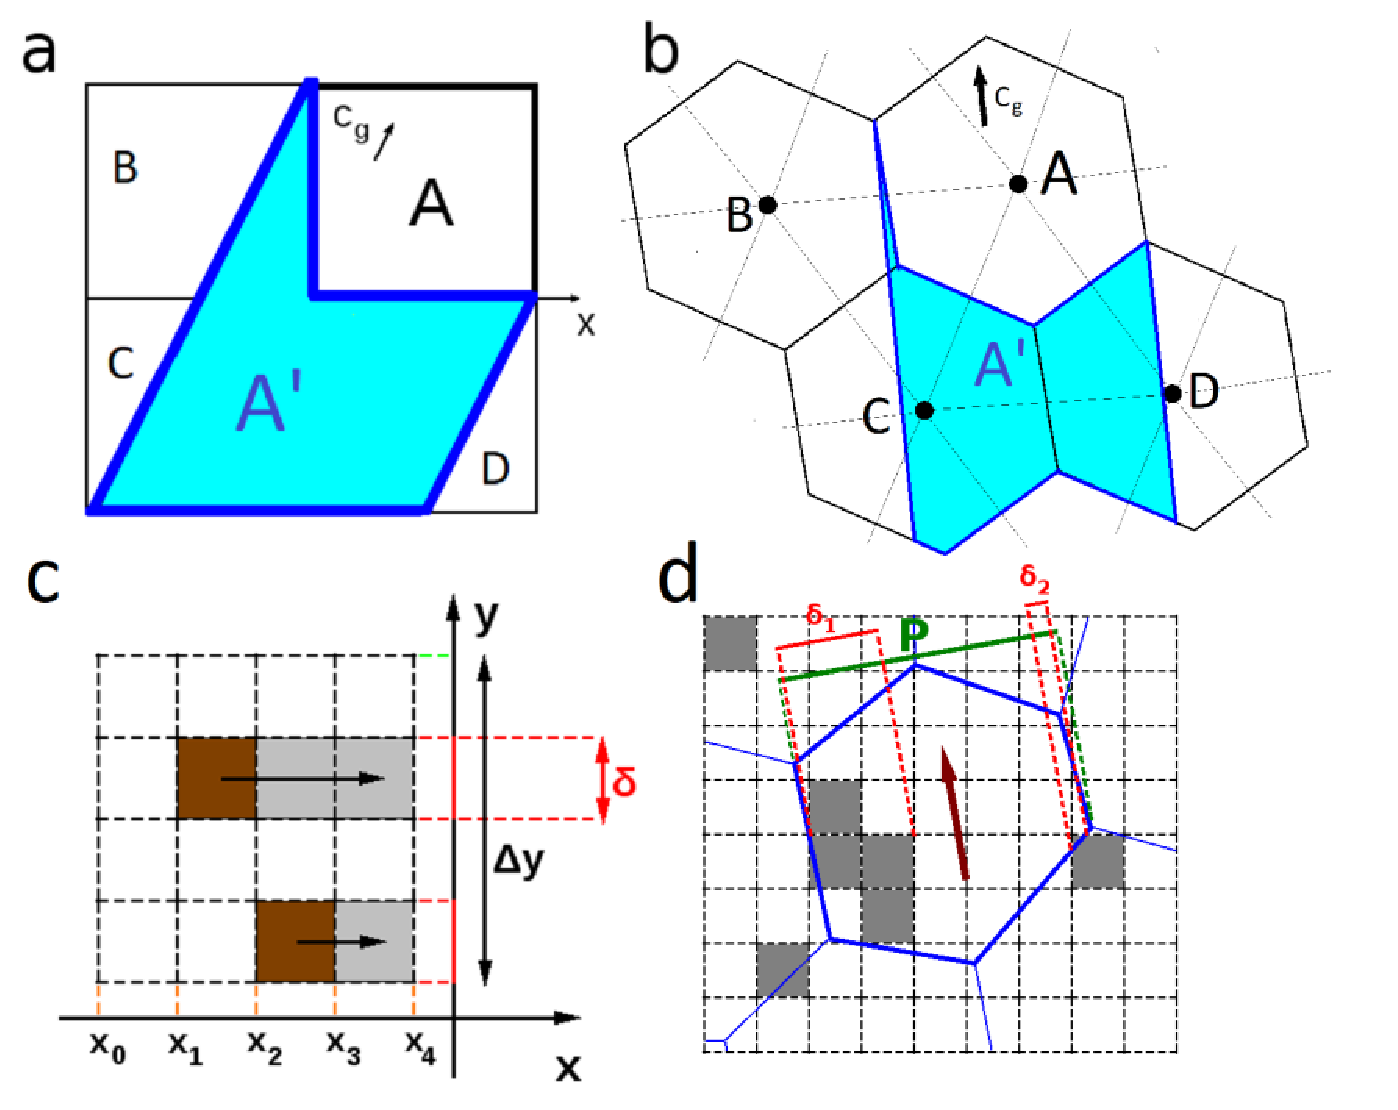
\epsfig{file=./eqs/UOST.eps,angle=0,width=4in}
\caption{
a：一个方形单元（A）及其上游多边形
（A\textsc{\char13}，由蓝线限定，以浅蓝色表示），对应以群速 $c_g$ 传播的谱分量。
联合 BCD 多边形表示邻域多边形。
b：同 a，但对应三角网格（六边形近似表示中值对偶单元）。
c：方形单元中 $\alpha$ 和 $\beta$ 的计算，$N_s=4$，谱分量沿 x 轴传播。
d：同 c，但对应六边形单元和倾斜谱分量。d 图中的灰色方块表示未解析障碍物。
}
\label{fig:UOST} \botline
\end{center}
\end{figure}

\textbf{网格参数的自动生成。}
开源 python 包 alphaBetaLab（https://github.com/menta78/alphaBetaLab）已被开发，
用于从真实世界水深自动估计上游多边形、透明度系数
$\alpha_l$、$\beta_l$、$\alpha_u$、$\beta_u$，以及 UOST 所需的其他参数。
alphaBetaLab 将单元视为自由多边形，并根据未解析障碍物相对于入射谱分量的横截面估计
透明度系数（图 \ref{fig:UOST}cd）。这意味着它可应用于任意类型网格，包括非结构三角
网格和 SMC 网格（截至 2018 年 8 月，仅处理规则网格和三角网格，但很快会加入对
SMC 网格的支持）。需要指出的是，虽然 UOST 本身能够使能量耗散随谱频率变化，但
alphaBetaLab 目前只考虑方向。关于 alphaBetaLab 中实现算法的更多细节，请用户参阅
\cite{art:Mentaschi2018a}。\cite{art:Mentaschi2018c} 提供了该软件及其架构的文档，
并给出了使用指导和示例。

\textbf{时间步设置。}
在 \ws\ 中，源项在每个全局时间步结束时施加。因此，为了在给定单元上正常工作，
UOST 要求全局时间步小于或等于该单元的临界 CFL 时间步，也就是最快谱分量完全穿过该
单元所需的时间。否则，部分能量会在未被阻挡的情况下穿过该单元 \citep{art:Mentaschi2018a}。

在单元大小差异很大的非结构网格中，如果把 UOST 应用于所有单元，包括最小单元，可能会
要求极小的全局时间步，从而影响模型经济性。为避免这一问题，用户可设置 alphaBetaLab
以忽略小于用户定义阈值的单元，然后在 \ws\ 中设置与该阈值相关的临界 CFL 时间步作为
全局时间步 \citep{art:Mentaschi2018c}。

\begin{table} \begin{center}
 \footnotesize
\begin{tabular}{|p{4cm}|p{2.5cm}|p{5.5cm}|} \hline \hline
Namelist 参数    &  说明           & 默认值 \\
\hline
  UOSTFILELOCAL &  局地 $\alpha$/$\beta$ 输入文件路径   &  obstructions\_local.\textit{gridname}.in    \\ \hline
  UOSTFILESHADOW &  阴影 $\alpha$/$\beta$ 输入文件路径   & obstructions\_shadow.\textit{gridname}.in   \\ \hline
  UOSTFACTORLOCAL &  局地透明度率定因子  &  1   \\ \hline
  UOSTFACTORSHADOW &  阴影透明度率定因子  &  1  \\
\hline
\end{tabular} \end{center}
\caption{UOST 参数、说明及默认值。} \label{tab:UOST}
\botline
\end{table}

\vsssub
\subsubsection{~$S_{xx}$：用户定义} \label{sec:XXx}
\vsssub

\opthead{XXn}{---}{user}

\noindent
这一位置预留给式~(\ref{eq:general_st}) 中尚未分类的源项。几乎按定义而言，
这里无法给出其具体形式。

\vssub
\subsection{~波-冰相互作用的源项}
\vsssub

波-冰相互作用过程已经是许多研究的主题。一般而言，波-冰相互作用需要描述海冰性质，
通常至少包括冰浓度（海洋表面被冰覆盖的比例）、平均冰厚和最大冰 floe 直径。实际上，
海冰常被破碎成许多块体（floes），其尺寸范围可以很宽，而这些尺寸会强烈改变色散以及
波-冰相互作用过程。

在当前版本的 \ww\ 中，处理海冰的不同选项代表了仍在推进的研究。目前有五种耗散过程版本，
分别由开关 {\code IC1}、{\code IC2}、{\code IC3}、{\code IC4} 和 {\code IC5}
启用；它们可与两种不同的散射效应版本 {\code IS1} 和 {\code IS2} 组合。第二种散射
程序是唯一使用最大 floe 直径的程序，因此也包含对海冰破裂、所得最大 floe 直径以及
部分滞回耗散的估计。

这些开关选择中的某些特性在应用时需要谨慎。例如，除冰浓度和冰厚外，强迫场是依赖上下文的：
它们在不同源项中具有不同含义。

目前还不能把为 frazil ice 或 pancake ice 设计的耗散参数化（{\code IC3} 或
{\code IC4}）与为冰盖设计的参数化（如 {\code IC2}）组合。此外，所有参数化尚未完全
整合：例如，在一些考虑海冰的修正色散关系中，floe 尺寸尚未被纳入。我们预计在 \ws\
未来版本中会有更流畅的方式来组合各种过程，可能会使用最大 floe 直径来调用不同程序。

在多数情况下，\ws\ 现在允许海冰相关输入具有空间和时间变率；但在实践中，这类信息通常
只对冰浓度（来自卫星或模型）和冰厚（多来自模型）可用。表示海冰性质的其他参数的变率，
用户通常很少能够获得。

观测研究海冰对波浪的影响很有挑战性；在冰缘及其附近对此类影响进行建模尤其困难，
其中非定常、非均匀输入冰场的精度可能成为精度的主要限制因素 \citep{rep:RPLA18}。
许多重要建模研究使用了 \ws\ 以外的模型，例如 \cite{art:DB13}。到目前为止，
\ws\ 中可用并在以下各节描述的各种选项，只在少数实际条件研究中得到测试，包括
\cite{art:LKS15}、\cite{art:Aea16}、\cite{art:WHR16}、\cite{art:RTS16}、
\cite{rep:RPLA18}、\cite{art:CRT17} 和 \cite{Liu2020}。

% Note: IC2 dispersion relation equation was moved to IC2 section

\noindent
用于表示海冰对波浪影响的实验性程序已经通过开关 {\code IC1}、{\code IC2}、
{\code IC3} 等实现。\ws\ 中最早实现的两个程序（由 \cite{rep:RO13} 实现）是
{\code IC1} 和 {\code IC2} 的初始版本；后者基于 \cite{art:LMC88} 和
\cite{art:LHV91} 的工作。这些效应可用复波数表示：

\begin{equation}\label{eq:waveno}
     {k} = {k_r} + i{k_i},
\end{equation}

\noindent
其中实部 ${k_r}$ 表示海冰对物理波长和传播速度的影响，会产生类似于水深地形导致的
变浅和折射效应；复波数虚部 ${k_i}$ 是指数衰减系数
${k_i}({x},{y},{t},\sigma $)（分别依赖位置、时间和频率），会造成波浪衰减。
${k_i}$ 通过 ${S_{ice}}/{E}=-2{c_g}{k_i}$ 引入，其中 ${S_{ice}}$ 为源项
（另见 \cite{bk:WAM94}, pg. 170）。对于提供 ${k_r}$ 的方法，例如 {\code IC2}、
{\code IC3} 和 {\code IC5}，海冰效应需要求解新的色散关系。

在 \ws\ 第 6 版中，海冰对 ${k_i}$ 的影响用于所有源函数：
{\code IC1}, ..., {\code IC5}。海冰对 ${k_r}$ 的影响已经为 {\code IC2} 和
{\code IC3} 实现，但只有 {\code IC3} 会把该影响导出给代码其他部分使用，这仍然是
实验性功能。

% Note : Is the above still true? Has it been done for IC2 now also?

冰源函数按冰浓度进行缩放。

对于海冰，最多允许五个输入参数作为非定常和非均匀场。这些参数可通称为
${C_{ice,1}}$、${C_{ice,2}}$、...、${C_{ice,5}}$。海冰参数的含义会随所选择的
${S_{ice}}$ 程序而变化。例如，在 {\code IC1} 的情况下，只指定一个参数
${C_{ice,1}}$。在某些情况下，如 {\code IC3} 和 {\code IC4}，也可选择更简单的
方式：输入与固定均匀情形相同的变量，并通过 namelist 参数定义。

关于如何使用新的海冰源函数，读者可参考回归测试 {\file ww3\_tic1.1-3} 和
{\file ww3\_tic2.1} 中的示例。

\textrm{\textit{\underline{在 {\file ww3\_shel} 中使用：}}}
允许非定常和非均匀输入海冰参数。当使用开关 {\code IC1}、{\code IC2}、{\code IC3}、
{\code IC5}、{\code BT8} 或 {\code BT9} 启用任一冰和泥沙源函数时，
{\file ww3\_shel} 会预期 8 个场的输入说明（5 个冰场，随后 3 个泥沙场）。
这些说明位于 ``water levels'' 信息之前。新场也可选择使用 {\file ww3\_shel.inp}
末尾附近的若干行指定为均匀场。

\textrm{\textit{\underline{在 {\file ww3\_multi} 中使用（\ws\ 第 6 版新增）：}}}
使用 namelist 方法向 {\file ww3\_multi} 提供说明时，现在可以在 {\file ww3\_multi}
中把泥沙和海冰系数指定为非定常和非均匀场。第 6 版以前，这只可在 {\file ww3\_shel}
中实现。不过，在撰写本文时，作者尚未测试通过 {\file ww3\_multi.nml} 读取这些说明
的新方法。

\textrm{\textit{\underline{源项的区分：}}}
源项 {\code IC1},...,{\code IC5} 预报波能耗散。海冰引起的波浪反射和散射
（例如 \cite{art:Wad75}）并不是耗散，而是保守过程。它们在 {\code IS1} 和
{\code IS2} 中单独处理。

\vsssub
\subsubsection{~$S_{ice}$：海冰阻尼（简单方法）} \label{sec:ICE1}
\vsssub

\opthead{IC1}{\ws/NRL}{E. Rogers and S. Zieger}

最先实现的方法（{\code IC1}）是由用户指定 ${k_i(x,t)}$；它在频率空间中均匀，
即 ${C_{ice,1}}={k_i}$。参数 ${C_{ice,2}}$,...,${C_{ice,5}}$ 不使用。
一个示例设置为 ${C_{ice,1}}=2\times 10^{-5}$。关于 {\code IC2} 和 {\code IC3}
的专门说明见后续各节。

{\code IC1} 的完整说明见 \cite{rep:RO13}，\cite{rep:RPLA18} 给出了简要总结。
这一简单方法曾用于 \cite{art:LKS15}，并被 \cite{art:RTS16}、\cite{rep:RPLA18}
和 \cite{rep:RMK18} 用作模型-数据反演程序的建模组成部分。

\vsssub
\subsubsection{~$S_{ice}$：海冰阻尼（Liu et al.）} \label{sec:ICE2}
\vsssub

\opthead{IC2}{\ws/NRL}{E. Rogers, S. Zieger, F. Ardhuin}

\noindent
这种表示波-冰相互作用导致波能耗散的方法，基于 \cite{art:LMC88}、\cite{art:LHV91}
和 \cite{art:Aea15}。主要输入海冰参数是冰厚（单位 m），它可在空间和时间上变化，
并作为强迫场 ${C_{ice,1}}$。

这是一个海冰覆盖导致衰减的模型，假定耗散由冰下边界层中的摩擦造成，并把海冰表示为
连续薄弹性板。\cite{art:LMC88} 的原始形式可通过把 {\code IC2} namelist {\F SIC2}
参数 {\code IC2DISPER = .TRUE.} 启用。该形式假定边界层始终为层流，但使用可在空间上
变化的涡黏性 ${\nu}$，它是强迫场 ${C_{ice,2}}$。

{\code IC2} 和 {\code IS2} 共享一个可选项，即使用 \cite{art:LMC88} 针对未破碎冰层
给出的色散关系：
\begin{equation}
\sigma^2 =  \left(gk_{ice} + B k_{ice}^5\right)  / \left(1/\tanh ( k_{ice}H) +\frac{\rho_{ice}  h k_{ice}} {\rho_{w} }\right),
\end{equation}
\begin{equation}
c_g =  (g+(5 + 4 k_{ice} M)Bk_{ice}^4)/(2\sigma(1+k_{ice}M)^2).
\end{equation}

\noindent
$B$ 和 $M$ 分别量化波浪导致的海冰弯曲效应和海冰惯性效应。由同一关系推导得到的冰下
群速在模块 {\code W3SIS2MD} 中使用，并在 {\code W3DISPMD} 中计算。细节见
\citet{art:LMC88}。

对于 {\code IC2}，色散关系定义为

\begin{equation}\label{eq:ice1}
  {\sigma}^2 = ({gk_r} + {Bk_r^5})/(\coth({k_r}{h_w}) + {k_r}{M}),
\end{equation}
\begin{equation}\label{eq:ice2}
  {c_g} = (g + (5 + 4{k_r}{M}){B}{k_r^4})/(2{\sigma}(1+{k_r}{M})^2),
\end{equation}
\begin{equation}\label{eq:ice3}
  {\alpha} = (\sqrt{{\nu\sigma}}{k_r)}/({c_g}\sqrt{2}(1+{k_r}{M})).
\end{equation}

\noindent
在本文记号中，$h_w$ 为水深，$h_i$ 为冰厚。变量 $B$ 和 $M$ 分别量化海冰弯曲和
海冰惯性的影响。二者都依赖 $h_i$ \citep[见][]{art:LMC88, art:LHV91}。

只有当 {\F MISC} namelist 中 ICEDISP=TRUE 时才会求解该方程。否则，
$k_{ice}=k$，与开阔水面相同。注意，$k_{ice}$ 的影响不会传回主程序。

\cite{art:SAG16} 通过加入一个更好的替代方案来表示涡黏耗散，从而改进了 {\code IC2}。
他们区分层流和湍流状态；把 {\code IC2DISPER = .FALSE.} 即可启用这一形式。在这种
情况下，耗散从层流形式（使用分子黏性并乘以经验调整因子 {\code IC2VISC}）过渡到
湍流形式（由因子 {\code IC2TURB} 放大），该过渡发生在 Reynolds 数高于用户定义阈值
{\code IC2REYNOLDS} 时。为考虑随机波场性质，该过渡会在范围 {\code IC2SMOOTH} 内
平滑处理。在湍流状态中，摩擦因子根据用户指定的冰下粗糙长度 {\code IC2ROUGH} 估计，
该长度预期为 $10^{-4}$~m 量级。
当 floe 直径远小于海洋波长时，还增加了对耗散率进行启发式削减的可能性
\citep[细节见][]{Aea18}。它基于如下假设：在这些条件下，冰 floe 至少部分跟随
水平运动，因此应减小用于估计耗散率的冰-水相对速度。该削减由 \cite{Aea18} 中称为
$r_D$ 的因子控制，其取值可通过 namelist 参数 {\code IC2DMAX} 设置。当波长长于
$D_{\max}/r_D$（$D_{\max}$ 为最大 floe 尺寸）时，耗散率会被削减；当最大 floe 直径
达到波长量级或更大时，则不削减。

参数 {\code IC2TURBS} 是南半球湍流耗散的经验增强项，引入它是为了测试偏差来源。
该参数将在未来版本中弃用。现在看来，把 IC2 与 IS2 中的非弹性耗散组合，可对两个半球
的主导波给出良好结果 \citep{Aea18}。

{\code IC2} 原始形式的完整说明见 \cite{rep:RO13}。它在 \cite{art:LKS15} 中得到应用。
\cite{rep:RPLA18} 给出了当前代码的简要总结。{\code IC2} 耗散机制改进的说明见
\cite{art:SAG16} 附录 B，该文也使用了这一改进。

\vsssub
\subsubsection{~$S_{ice}$：海冰阻尼（Shen et al.）} \label{sec:ICE3}
\vsssub

\opthead{IC3}{Clarkson U. Fortran-77 code}{E. Rogers, X. Zhao, S. Cheng, S. Zieger}

\noindent
第三种表示波-冰相互作用的方法来自\linebreak
\cite{art:WS10}。该模型把海冰视为黏弹性层。${C_{ice,1}}$ 用于冰厚（m）；
${C_{ice,2}}$ 用于黏性（$\mathrm{m^2\,s^{-1}}$）；${C_{ice,3}}$ 用于密度
（$\mathrm{kg\,m^{-3}}$）；${C_{ice,4}}$ 用于有效剪切模量（Pa）；
${C_{ice,5}}$ 不使用。一个示例设置为
${C_{ice,1...4}}=[0.1, 1.0, 917.0, 0.0]$。

在 \ws\ 第 4 版中，这一 $S_{ice}$ 方法（{\code IC3}）比 {\code IC1} 或 {\code IC2}
昂贵得多。模型 5.16 版基本解决了这一问题。

模型 5.16 版引入了 namelist {\F SIC3}。Namelist 参数汇总如下，其中一些参数会在
后文进一步讨论。

\begin{clist}
\cit {IC3CHENG} {5.16 版新增的求解技术。默认值 = {\code TRUE}。}
\cit {IC3HILIM} {冰厚的可选限制器。默认值=100（即默认不使用该选项）。}
\cit {IC3KILIM} {耗散率 ${k_i}$ 的可选限制器。默认值=100（即默认不使用该选项）。}
\cit {USECGICE} {设为 {\code TRUE} 时，模型将包含海冰对群速的影响。默认值 = {\code FALSE}。}
\cit {IC3VISC} {若用户希望使用常数且均匀的有效黏性，现在可通过 namelist 设置。默认=N/A。}
\cit {IC3ELAS} {同 {\code IC3VISC}，但用于有效弹性。默认=N/A。}
\cit {IC3DENS} {同 {\code IC3VISC}，但用于海冰密度。默认=N/A。}
\cit {IC3HICE} {同 {\code IC3VISC}，但用于冰厚。默认=N/A。}
\cit {IC3MAXCNC} {可用于在某些冰况下切换到另一种耗散的参数（见下文）。默认=100（即不使用该选项）。正常范围为 0 到 1。}
\cit {IC3MAXTHK} {同上。默认=100（即不使用该选项）。正常范围为 0 到 10 m。}
\cit {IC2REYNOLDS} {与 IC2 非色散湍流边界层方案相关的参数。默认=1.5e+5。}
\cit {IC2ROUGH} {同上。默认=0.02。}
\cit {IC2SMOOTH} {同上。默认=7.0e+4。}
\cit {IC2VISC} {同上。默认=2.0。}
\cit {IC2TURB} {同上。默认=2.0。}
\cit {IC2TURBS} {同上。默认=0.0。}
\end{clist}

{\code IC3CHENG} 选项是模型第 5 版新增的。设为 {\code TRUE} 时，模型将使用由
S. Cheng 提供的替代求解技术。它有两个重要特点。第一，稳定性得到改善，因此不需要
使用冰限制器，即 {\code IC3HILIM} 参数。第二，该方法要求四个海冰流变参数中的三个
是定常且均匀的，并通过 namelist 参数输入（见下文）。

若 {\code IC3CHENG} 设为 {\code FALSE}，建议用户使用冰厚限制器 {\code IC3HILIM}
以保证稳定性（建议取 25 到 100 cm）。参数 {\code IC3KILIM} 曾在 \ws\ 某些早期
开发版本中用于稳定且快速的计算，但现在已无必要，用户可忽略。

在模型 4.18 版中，四个海冰流变参数（冰厚、有效黏性、有效弹性和冰密度）允许为
非定常和非均匀场。这可通过 {\file ww3\_prep} 提供。或者，当使用 {\file ww3\_shel}
且不需要非均匀输入时，可用 {\file ww3\_shel} 的 ``homogeneous'' 选项输入流变参数。
模型 5.16 版新增了通过 namelist {\F SIC3} 指定四个海冰流变参数的选项。这里有两个
限制：1) 若 {\code IC3CHENG} 设为 {\code FALSE} 且 {\code USECGICE} 设为
{\code TRUE}，则不能使用 namelist 方法；2) 若 {\code IC3CHENG} 设为 {\code TRUE}，
则三个流变参数（有效黏性、有效弹性和冰密度）必须使用 namelist 方法。若
{\code IC3CHENG} 设为 {\code TRUE} 或 {\code USECGICE} 设为 {\code FALSE}，
第四个海冰流变参数（冰厚）可由任一方法输入（namelist 或非 namelist）。模型会执行
错误检查，以确保用户只用一种方法为每个参数指定输入（不会假定某种输入方法优先于另一种）。

海冰修正后的 ${k_r}$ 通过左端的 $c_g$（群速）和 $c$（相速）计算纳入控制方程
(\ref{eq:bal_plane})；例如 \citet[][以及后续未发表工作]{art:RH09}。波数和群速的
修正可选择传回主程序，从而产生类似于水深地形导致的折射和变浅效应。不过，到目前为止，
该功能只用于学术研究，而非现实情景的常规应用。\\

要启用变浅效应，模型应使用 namelist 变量 {\code USECGICE = TRUE}。要启用折射效应，
模型应使用开关 {\code REFRX} 编译。使用该开关时，模型基于包含海冰效应的相速空间梯度
计算折射，而不是使用无冰的简化波浪色散关系。代码附带的回归测试 {\file ww3\_tic1.3}
演示了这些效应。

当冰厚为零时，使用 {\code IC3CHENG} 求解器得到的群速不会完全退化为开阔水面色散关系
给出的群速。这是由计算 $c_g = \frac{\partial \sigma}{\partial k} =
\frac{\Delta \sigma}{\Delta k} $ 时的数值误差造成的。如果启用这些效应，群速中的这些
小差异会导致轻微的变浅和折射误差。发现冰厚为零时误差小于 10\%，且依赖频率。现在通过
在冰厚恰为零时跳过求解器来避免这一问题。若冰厚接近但不恰为零，则这一差异可能仍可见。
尚未测试 CHENG 解在其他参数（有效黏性、有效剪切模量）趋近零时的行为。对于相同海冰输入，
{\code IC3CHENG} 设为 {\code FALSE} 与 {\code TRUE} 时的解之间，也已注意到虽小但
实质性的差异。

如上所述，{\code USECGICE = TRUE} 是产生变浅效应所必需的。不过，由于某些海冰流变
会导致群速增大，建议用户谨慎使用这一选项。群速会影响 CFL 准则，这可能要求用户减小
时间步长。对于不希望处理这一问题的用户，推荐使用 {\code USECGICE = FALSE}。

在模型 5.16 版中，新增了一个非默认选项，使耗散参数化在某些冰况下发生改变。若冰浓度
超过 {\code IC3MAXCNC} 且冰厚超过 {\code IC3MAXTHK}，则使用 {\code IC2} 耗散
（更具体地说，是 {\code IC2} 的非默认、非色散边界层方案子选项），以替代
\cite{art:WS10} 的基于色散的耗散估计。更多信息见 {\code IC2} 说明。由于该特性是
非色散的，不应与 {\code USECGICE = TRUE} 一起使用。

{\code IC3} 最早出现在 \ww\ 第 4 版中，最初的简单测试见 \cite{pro:RZ14}。随后它已
用于 \cite{art:LKS15}、\cite{art:WHR16}、\cite{art:RTS16} 和 \cite{art:CRT17}。

\vsssub
\subsubsection{~$S_{ice}$：海冰经验/参数化阻尼} \label{sec:ICE4}
\vsssub

\opthead{IC4}{\ws/NRL}{C. Collins and E. Rogers}

\noindent
海冰导致波浪阻尼的第四个选项（{\code IC4}）最早由 \cite{rep:CR17} 引入。
它提供若干简单经验/参数化形式之一，用于实现海冰造成的波能耗散。{\code IC4} 的动机
是提供一个简单、灵活且高效的源项，以一种高度参数化的方式再现波-冰相互作用的一些
基本物理。具体方法由 namelist 参数 {\code IC4METHOD} 的整数值设定（目前为 1 到 10）。
前六个方法为：1) 对 \cite{art:WAD88} 现场数据的指数拟合；2) \cite{art:MBK14}
中的多项式拟合；3) \cite{art:HT15} 中给出的、对 \cite{art:KM08} 计算结果的二次拟合；
4) \cite{art:Ko14} 的式 1；5) 最多 4 个阶梯的简单阶跃函数（可为非定常和非均匀）；
6) 最多 10 个阶梯的简单阶跃函数（必须定常且均匀）。方法 7、8 和 9 使用依赖频率和
冰厚的多变量幂律拟合。除 {\code IC4} 的第四种方法外，所有方法都具有依赖频率的衰减。
第四种方法中，衰减随波高变化，但在频率空间中均匀。

下文用 {\code IC4M1} 表示 {\code IC4} 方法 1，依此类推。{\code IC4} 出现在
{\file switch} 中，而 namelist {\code IC4METHOD=1}（例如）出现在文件
{\file ww3\_grid.inp} 中。与 {\code IC1} 中 ${C_{ice,1}}$ 为用户确定的衰减不同，
这里 ${C_{ice,n}}$ 的含义依赖上下文。对于 {\code IC4M1}、{\code IC4M2} 和
{\code IC4M4}，${C_{ice,n}}$ 是方程常数。对于 {\code IC4M3}、{\code IC4M7}、
{\code IC4M8} 和 {\code IC4M9}，${C_{ice,1}}$ 为冰厚。对于 {\code IC4M5}，
${C_{ice,n}}$ 控制阶跃函数。对于 {\code IC4M6}，namelist 变量控制阶跃函数。
注意，对于会使用 ${C_{ice,n}}$ 的方法，用户可用类似输入水位的方法，将其作为
非定常和非均匀场提供。

{\code IC4M1}：选择一个指数方程拟合 \cite{art:WAD88} 表 2 中的数据，结果会优先
衰减高频波。这参数化了众所周知的海冰低通滤波效应。方程形式如下：
\begin{equation}\label{eq:ice1}
  {\alpha} = \exp\left[\frac{-{2\pi}C_{ice, 1}}{{\sigma}} - C_{ice, 2}\right]
\end{equation}

\noindent 这里，$\alpha$ 是能量的指数衰减率，为振幅衰减率的两倍：
$\alpha = 2k_i$。由数据确定的数值为 ${C_{ice,1...2}}=[0.18, 7.3]$，但用户可以修改。
该方法在 \cite{rep:CR17} 中有说明和应用。

{\code IC4M2}：该方法使用用户指定的多项式表示耗散。它很有力，因为可表示许多形状，
例如拟合基于观测的耗散率。该方法在 \cite{rep:CR17} 中有说明和应用。方程为
\begin{equation}\label{eq:ice2}
  {\alpha} = C_{ice,1} + C_{ice,2}\left[{\frac{\sigma}{2\pi}}\right] + C_{ice,3}\left[{\frac{\sigma}{2\pi}}\right]^2 + C_{ice,4}\left[{\frac{\sigma}{2\pi}}\right]^3 + C_{ice,5}\left[{\frac{\sigma}{2\pi}}\right]^4
\end{equation}

\noindent
若用户希望遵循 \cite{art:MBK14}，建议系数为
${C_{ice,1...5}}=[0, 0, 2.12\times 10^{-3}, 0, 4.59\times 10^{-2}]$。
其他建议多项式见 \cite{rep:RMK18}。

采用合适系数时，该多项式方法可再现所谓的 ``roll-over effect''，即衰减在频率空间中
非单调。不过，一些近期研究并未显示这一效应，例如 \cite{art:RTS16} 和 \cite{art:LK17}；
它也可能只是早期观测研究中的虚假伪影。

虽然 ${C_{ice,1...5}}$ 可指定为随时间和空间变化，但实践中很少使用这一特性。多数用户
会偏好使用常数值；为方便起见，这些值可通过 namelist 参数设置，其中 $C_{ice,i}$
在 {\code SIC4} namelist 中指定为 {\code IC4CN(i)}，而不是通过 {\file ww3\_prep}
等作为输入场给出。

{\code IC4M3}：\cite{art:HT15} 将一个二次方程拟合到 \cite{art:KM08} 计算的衰减系数，
该衰减系数是频率、$T$ 和冰厚 $h$ 的函数。较厚的冰和较高频率（较短周期）会使衰减增大。
二次方程的系数数量多到不适合由用户指定，因此方程被硬编码，可调参数 ${C_{ice,1}}$
为冰厚 $h$。该方法在 \cite{rep:CR17} 中有说明和应用。作为参考，方程如下：
\begin{equation}\label{eq:ice3}
  {\ln{\alpha(T,h)}} = -0.3203 + 2.058h - 0.9375T - 0.4269h^2 + 0.1566hT + 0.0006T^2
\end{equation}

\noindent
关于 {\code IC4M3} 有四点警告。第一，该方程本身是对 \cite{art:KM08} 中用于计算
衰减系数的原始 $h$ 范围（0.5 到 3 m）的外推，见 \cite{art:HT15}。第二，在
\cite{art:KM08} 中，预测的波浪衰减基于散射（保守过程），而在 {\code IC4M3} 中，
波浪衰减被当作耗散（非保守）处理。第三，不建议把 {\code IC4M3} 与散射程序
{\code IS1} 或 {\code IS2} 组合使用，因为这会把散射重复计入。第四，实现中假定每米
遇到一个 floe，这不同于 \cite{art:HT15} 中允许该长度尺度变化的处理。更多细节请参阅
{\file w3sic4md.F90} 中的内联文档。

{\code IC4M4}：\cite{art:Ko14} 发现衰减是有效波高的函数。衰减随 ${H_s}$ 线性增大，
直到 ${H_s} = 3$ m，此后衰减封顶，即
\begin{equation}
\left \{
\begin{array}{llrcl}
{\frac{\partial H_s}{\partial dx}} = {C_{ice,1}}\times {H_s}   & & \text{for} \> {H_s} \leq 3 \text{ m}  \\
{\frac{\partial H_s}{\partial dx}} = {C_{ice,2}}               & & \text{for} \> {H_s} > 3 \text{ m}     \\
\end{array} \right .
\end{equation}
其中 {$k_i=\frac{\partial H_s}{\partial dx}/H_s$}。

\cite{art:Ko14} 给出的数值为 ${C_{ice,1...2}}=[5.35\times 10^{-6}, 16.05\times 10^{-6}]$。
示例见回归测试 {\file ww3\_tic1.1/input\_IC4\_M4}。该方法在 \cite{rep:CR17}
中有说明和应用。

{\code IC4M5}：这是一个最多 4 个阶梯的简单阶跃函数。它由可选的非定常和非均匀参数
${C_{ice,1...7}}$ 控制。参数 ${C_{ice,1...4}}$ 控制阶梯水平，单位为耗散率
${k_i}$。参数 ${C_{ice,5...7}}$ 控制阶梯边界（单位 Hz）。示例见回归测试
{\file ww3\_tic1.1/input\_IC4\_M5}。该方法见 \cite{rep:CR17}。

{\code IC4M6}：这是一个最多 10 个阶梯的简单阶跃函数。它由定常且均匀的 namelist
参数 {\code IC4KI} 和 {\code IC4FC} 控制。数组 {\code IC4KI} 控制阶梯水平，
其单位为弧度每米的耗散率 ${k_i}$。数组 {\code IC4FC} 控制阶梯边界（单位 Hz）。
示例见回归测试 {\file ww3\_tic1.1/input\_IC4\_M6}。

{\code IC4M7}：这是 \cite{art:Dob15} 给出的耗散公式，针对 pancake ice 与 frazil ice
混合物开发，使用了南极 Weddell 海收集的数据。公式依赖波频率和冰厚：
\begin{equation}\label{eq:ice7}
  {\alpha=2k_i=0.2h^1f^{2.13}} \:\:\: .
\end{equation}
该方法见 \cite{rep:RPLA18}。

{\code IC4M8}：与 {\code IC4M7} 类似，该方法具有如下通用形式：
\begin{equation}\label{eq:ice8}
  {k_i=C_{hf}h^mf^n} \:\:\: .
\end{equation}
该公式取自 \cite{Meylan2018}，其中称为 ``Model with Order 3 Power Law''。
\cite{Liu2020} 应用了该公式，并称其为 ``M2'' 模型。该模型规定 $m=1$、$n=3$，
$C_{hf}$ 为用户指定的率定系数。\cite{Liu2020} 为两个现场案例提供了率定，
\cite{rep:RYW2021} 则为第三个现场案例 \cite{art:RMK2021} 提供了率定。第三个率定
被设为 {\code IC4M8} 的默认值，$C_{hf}=0.059$，但可通过 namelist 参数
{\code IC4CN}（常数且均匀设置）修改，也可使用空间和/或时间变化参数 ${C_{ice,2}}$。
关于这些率定的更多细节见 {\file w3sic4md.F90} 中的内联文档。该方法在功能上与
{\code IC5} 中的 ``{\code M2}'' 模型相同（即 {\code IC5} 且 {\code IC5VEMOD=3}），
这里只是作为 {\code IC4M8} 冗余纳入，因为它与 {\code IC4M7} 和 {\code IC4M9}
同属式 (\ref{eq:ice8}) 形式的 ``family''。

设置 namelist 参数的示例见 {\file /regtests/ww3\_tic1.1/input\_IC4\_M8}。

{\code IC4M9}：该公式取自 \cite{rep:RYW2021} 第 2.2.3 节给出的 ``monomial power fit''。
与 {\code IC4M7} 和 {\code IC4M8} 一样，它是式 (\ref{eq:ice8}) 通用形式的一个特例。
其特殊性在于约束 $m=n/2-1$。\cite{rep:RYW2021} 通过调用 \cite{art:YRW2019} 的缩放
关系推导了这一约束；该缩放基于以冰厚为相关长度尺度的 Reynolds 数。\cite{art:YRW2022}
的方程 2 中也给出了该关系。默认 namelist 设置为 $C_{hf}=2.9$ 和 $n=4.5$，来自
\cite{rep:RYW2021} 和 \cite{art:YRW2022} 针对 \cite{art:RMK2021} 的率定。更多细节
（包括 \cite{art:Yu2022} 等替代率定）见 {\file w3sic4md.F90} 中的内联文档。
常数值可用 namelist 参数设置，其中 $C_{hf}$ 和 $n$ 分别为 {\code IC4CN(1)}
和 {\code IC4CN(2)}。同一组量的空间和/或时间变化可分别用 ${C_{ice,2}}$ 和
${C_{ice,3}}$ 指定。

{\code IC4M8} 和 {\code IC4M9} 中 namelist 默认的 $C_{hf}$ 值，与
\cite{man:SWAN4145A} 中实现的相同公式一致。

{\code IC4M10} 是一种由海冰 floe 散射造成衰减的方法，依赖冰厚和 floe 尺寸，
基于 \cite{art:MHB21}。

\vsssub
\subsubsection{~$S_{ice}$：海冰阻尼（有效介质模型）} \label{sec:ICE5}
\vsssub

\opthead{IC5}{U. of Otago MATLAB code}{Q. Liu, E. Rogers, A. Babanin}

\noindent
表示海冰诱导波浪衰减的第五个选项（{\code IC5}）由 \citet{Liu2020} 引入。它提供
三种不同模型来估计衰减率 $k_i$，包括两个黏弹性（VE）梁模型 \citep{art:MMS15}
和一个黏性模型 \citep{Meylan2018}。

两个 VE 模型，即扩展 Fox and Squire 模型 \citep[下文称 EFS 模型；另见][]{art:FS1994}
以及 Robinson and Palmer 模型 \citep[][下文称 RP 模型]{Robinson1990}，都把无限长
漂浮冰层描述为均匀 VE 介质，其特征由两个\emph{经验}流变参数表示，即冰层弹性剪切模量
$G$ 和冰层黏性 $\eta$。在这一框架下，色散关系修正为 \citep{art:MMS15}：
\begin{equation}
Q g \kappa \tanh(\kappa d)-\sigma^2 = 0,
\label{eq:vedisp}
\end{equation}
其中 $d$ 为水深，$\kappa = k_r + i k_i$ 为冰耦合波的复波数。实部
$k_r = 2\pi / \lambda$ 表征海冰对波长的影响，$k_i$ 为波振幅衰减率。
式 (\ref{eq:vedisp}) 中 EFS 和 RP 模型的 $Q$ 项为

\begin{align}
Q_{EFS} &= \frac{G_{\eta} h_i^3}{6 \rho_w g} (1+\nu) \kappa^4 - \frac{\rho_i h_i \sigma^2}{\rho_w g} + 1,\label{eq:fsdisp}\\
%
Q_{RP}  &= \frac{G h_i^3}{6 \rho_w g} (1+\nu) \kappa^4 - \frac{\rho_i h_i \sigma^2}{\rho_w g} + 1 - i \frac{\sigma \eta}{\rho_w g}.\label{eq:rpdisp}
\end{align}
这里 $\rho_w$（$\rho_i$）为水（海冰）密度，$h_i$ 为冰盖厚度，
$G_{\eta}=G- i \sigma \rho_i \eta$ 为复剪切模量，$\nu \simeq 0.3$ 为海冰 Poisson 比。
EFS 模型中的黏性参数 $\eta$ 具有运动黏性的量纲（单位：m$^2$ s$^{-1}$），而 RP 模型
中的 $\eta$ 表示单位面积、单位速度上的常数黏性阻尼力
\citep[单位：kg m$^{-2}$ s$^{-1}$；][]{Meylan2018}。由于二者高度相似，
式 (\ref{eq:fsdisp}) 和 (\ref{eq:rpdisp}) 可用同一个 Newton-Raphson 迭代求解器计算
\citep[见][]{Liu2020} 的附录。

通过详细理论分析，\citet{Meylan2018} 指出，在假定 $k_r$ 与开阔水面波数 $k_0$
偏离不大、且衰减率 $k_i$ 较弱时，上述两个 VE 模型预报
\begin{align}
k_i^{EFS} &\propto \eta h_i^3 \sigma^{11},\label{eq:fspw}\\ k_i^{RP} &\propto \frac{\eta}{\rho_w g^2} \sigma^3,\label{eq:rppw}
\end{align}
而先前现场测量 \citep[e.g.,][]{Meylan2018, RMK21} 支持幂律 $k_i \propto \sigma^n$，
其中 $n$ 在 2 到 4 之间。式~(\ref{eq:fspw}) 和 (\ref{eq:rppw}) 表明，在某些状态下
（即 $k_r \approx k_0$ 且 $k_i$ 较低），EFS 模型的 $k_i$ 对波频率过于敏感，而 RP
模型的 $k_i$ 不显示对冰厚的依赖。

{\code IC5} 模块包含的第三个模型基于 \citet[][其第 6.2 节；下文称 M2 模型]{Meylan2018}
提出的 ``Model with Order 3 Power Law''。该模型假设波能损失与水平冰速平方乘以冰厚
成正比。衰减率为
\begin{equation}
k_i^{M2} = \frac{\eta h_i}{\rho_w g^2} \sigma^3,
\label{eq:m2pw}
\end{equation}
其中 $k_i$ 随 $h_i$ 线性缩放，这类似于 \citet{art:Dob15} 在 pancake ice 下收集的
现场测量；$\eta$ 的单位为 kg m$^{-3}$ s$^{-1}$。

与 {\code IC3} 相同，{\code IC5} 需要四个海冰输入参数：$C_{ice, 1}$ 为冰厚 $h_i$
（m），$C_{ice, 2}$ 为\emph{有效}黏性 $\eta$（单位随所选模型而变化，见上文），
$C_{ice, 3}$ 为冰密度 $\rho_i$（kg m$^{-3}$），$C_{ice, 4}$ 为\emph{有效}剪切模量
$G$（Pa）\footnote{该参数与 M2 模型无关；选择 M2 模型时可简单使用 $G=1$ Pa。}。
\citet{Liu2020} 给出了 {\code IC5} 模块在两个案例研究中的应用。关于如何使用该海冰
模块的示例，请读者参阅该论文和回归测试 {\code ww3\_tic1.1}。

Namelist {\F SIC5} 包含下列参数：
\begin{clist}
\cit{IC5MINIG} {允许的最小剪切模量 $G$；默认= 1 Pa（即不允许零 $G$）。}
%
\cit{IC5MINWT} {允许的最小波周期 $T$；默认=0 s（即默认不使用该选项）。}
%
\cit{IC5MAXKRATIO} {允许的最大 $k_{ow}/k_r$，其中 $k_{ow}$ 为开阔水面波数；默认=1E9（即默认不使用该选项）。}
%
\cit{IC5MAXKI} {允许的最大 $k_i$；默认=100 m$^{-1}$（即默认不使用该选项）。}
%
\cit{IC5MINHW} {允许的最小水深 $d$；默认=0 m（即默认不使用该选项）。}
%
\cit{IC5MAXITER} {允许的最大迭代次数；默认=100。}
%
\cit{IC5VEMOD} {要选择的海冰模型：1 - {\code EFS}，2 - {\code RP}，3 - {\code M2}；默认=3（即\textbf{选择 {\code M2} 模型}）。}
\end{clist}
前 6 个参数被引入以提高 EFS 模型数值求解器的稳定性
\citep[在少数情况下，特别是水深 $d$ 较浅且 $G$ 较低时，求解器可能在短波周期下失败；见][]{Liu2020}。
不过，自 7.12 版起，M2 模型成为默认选项，因此默认不使用这些限制器。

\vsssub
\subsubsection{~$S_{is}$：海冰扩散散射（简单方法）} \label{sec:IS1}
\vsssub

\opthead{IS1}{\ws/NRL}{S. Zieger}

\noindent
海冰对波浪的非保守效应已通过开关 {\code IC1} 到 {\code IC3} 实现（见
\para\ref{sec:ICE1}--\ref{sec:ICE3}）。海冰的保守效应已在开关 {\code IS1}
中实现，表示一种简单的散射形式。假定 floe 尺寸小于网格尺寸，并且入射波能的一部分
$\alpha_{ice}$ 会各向同性地散射。该比例由海冰浓度 ICE 通过一个简单线性传递函数确定：
\begin{equation}\label{eq:IS101}
     \alpha_{ice} = \max\left \{0 , C_1\ \mathrm{ICE} + C_2 \right \} \:\:\: .
\end{equation}

\noindent
系数 $C_1$ 和 $C_2$ 可通过 namelist {\F SIS1} 中的 namelist 参数 {\code ISC1}
和 {\code ISC2} 定制。在每个离散频率和方向上，波能按 $\alpha_{ice}$ 的量减少，
并重新分配到同一离散频率的所有方向上，以守恒能量。

\vsssub
\subsubsection{~$S_{is}$：依赖浮冰尺度的散射与耗散} \label{sec:IS2}
\vsssub

\opthead{IS2}{\ws}{F. Ardhuin, C. Sevigny, G. Boutin,  D. Dumont,  T. Williams}


该散射项的实现总体遵循 \cite{art:MM06} 的方法，并加入了对波浪破碎海冰的估计，以便更新最大浮冰直径。最后，还把一种基于蠕变的耗散同散射结合起来。


散射源项由散射系数 $\beta_{\mathrm{is},\mathrm{MIZ}}(\theta-\theta')$ 定义；默认情况下它是各向同性的，但可通过在 {\F SIS2} namelist 中设置 {\code IS2ISOSCAT=FALSE} 赋予任意方向依赖性。因此源项为
\begin{equation}
 \frac{S_{\mathrm{is}}(k,\theta)}{\sigma} =  \int_0^{2\pi}\beta_{\mathrm{is},\mathrm{MIZ}}(\theta-\theta') [s_\mathrm{scat}  N(k,\theta')-N(k,\theta)] d\theta'  .
 \end{equation}
其中 $s_\mathrm{scat}$ 默认设为 1.0，但可由 {\F SIS2} namelist 中的 {\code IS2BACKSCAT} 修改。\\


散射系数 $\beta_{\mathrm{is},\mathrm{MIZ}}$ 的确定基于理论反射系数 $\alpha_n(\sigma,h)$，该系数对应正入射波从开阔水域半平面传播到冰厚恒定为 $h$ 的覆冰水域半平面。由 \cite{art:KM08}（若 {\code IS2WIM1=0.}）或 \cite{art:Ben12}（若 {\code IS2WIM1=1.}）计算的 $\alpha_n(\sigma,h)$ 值制表存放在 {\code W3SIS2MD} 模块中。按照 \cite{art:Dea11}，破碎海冰被视为一系列这样的冰-水界面。忽略多次反射时，散射参数化把单位时间衰减定义为：网格单元中覆冰部分相当于由平均直径 $D_{m}$ 的一串浮冰组成，每块浮冰产生部分反射 $\alpha_n(\sigma,h)$，即
\begin{equation}
\beta_{\mathrm{is},\mathrm{MIZ}}=c_i~c_g \alpha_n(\sigma,h) / D_{m},
 \end{equation}
其中 $c_i$ 为冰密集度。\\
 

平均浮冰直径 $D_m$ 的估计基于如下假定：直径为 $D$ 的浮冰数量服从正比于 $D^{-\gamma}$ 的幂律。进一步假定该幂律适用于从最小值 $D_{\min}$ 到最大值 $D_{\max}$ 的 $D$ 范围。因此平均值为
\begin{equation}
D_m=\frac{\gamma}{\gamma -1}\times\frac{D_{\max}^{-\gamma +1}-D_{\min}^{-\gamma +1}}{D_{\max}^{-\gamma}-D_{\min}^{-\gamma}}.
\label{analytic_Dbar}
\end{equation}

\noindent
目前 $D_{\min}$ 为用户给定值。$D_{\max}$ 可作为强迫场提供，例如来自海冰模式或观测；或者当 namelist 参数 {\code IS2BREAK} 设为 {\code TRUE} 时，由局地波场对海冰的破裂估计得到。如果 namelist 参数 {\code IS2DUPATE} 设为 {\code TRUE}，即使波浪后来小到无法把海冰破裂到该尺度，较小的 $D_{\max}$ 仍会保持。在有外部强迫/耦合可用时（例如海冰模式中的海冰性质平流），这可能是合适的模式用法。相反，如果 {\code IS2DUPDATE} 设为 {\code FALSE}，$D_{\max}$ 将始终调整到局地海况，即使这意味着增大 $D_{\max}$。\\


假定波长为 $\lambda$ 的波浪破碎海冰后产生直径为 $\lambda / 2$ 的浮冰。在该参数化中，若满足以下三个条件，则发生波浪破冰 \citep{art:Wea13}：
\begin{enumerate}
\item $\lambda/2 \geq D_{\min} \quad \mathrm{and} \quad  \lambda/2 \leq D_{\max}$
\item $D_{\max}>D_c$，因为存在一个取决于海冰性质的临界直径，低于该直径时不可能发生弯曲破坏
\item $\varepsilon>\varepsilon_c$，入射波导致的应变必须大于给定临界应变
\end{enumerate}
第一个条件只是检查新的 $D_{\max}$ 值将大于 $D_{\min}$ 且小于先前的 $D_{\max}$。\\

第二个条件基于 \cite{inc:M86}，并采用 \cite{art:Bea18} 给出的修正，其中 $D_{c}$ 定义为
\begin{equation}
D_{c}=\dfrac{1}{2}\left(\frac{\pi^4 Y^* h^3}{48 \rho g (1 -\nu ^2)}\right)^{1/4}. 
\end{equation}

第三个条件对应弯曲应变阈值。波浪造成的水平应变与冰层曲率有关，在一维情况下为 $\varepsilon = 0.5 h \partial ^2 \eta_{\mathrm ice} / \partial x^2$。应变方差为
\begin{equation}
\langle\varepsilon^2\rangle = \left( \frac{h}{2} \right) ^2   \int_{k_1}^{k_2} k_{ice}^4 F(k)dk ,
\label{strain_sign}
\end{equation}
其中 $h$ 为冰厚，$k_{ice}$ 为波数 $2 \pi /\lambda_{ice}$。借鉴波浪破碎思想 \citep{art:BBY00}，曲率方差的积分限制在局地波数 $k_{\mathrm ice}$ 附近。还需注意，我们定义了一个有效最小冰厚 $h_{\min}$，使得若 $h<h_{\min}$，应变方差用 $h=h_{\min}$ 计算，以避免模式中出现与通常观测不符的“不可破碎”弹性薄冰。因此，我们把 $D_{\max}$ 取为满足以下判据的最短波的半波长：
\begin{equation}
F_{break}\, \sqrt{\varepsilon^2} > \frac{\sigma_c}{Y^*} ,
\label{strain_crit}
\end{equation}
其中 $\sigma_c$ 为海冰弯曲强度。$F_{break}$ 是表示随机波作用的因子，可通过 {\F SIS2} namelist 参数 {\code IS2BREAKF} 调整。理论上它应取决于海冰受波浪强迫的持续时间；基于 500 个 Rayleigh 分布波中的典型最大值，取 $F_{break}=3.6$。因此 $F_{break} \, E_s$ 为随机波的最大应变。\\




非弹性或非完全弹性耗散被包含在该例程而不是 ICn 中，因为它强烈依赖浮冰尺度。按照 \cite{art:Bea18}，假定浮冰变形并非完全弹性，且波浪诱导的循环应变和应力会把波能耗散为热。冰的循环变形可能需要远大于重力位能的弹性能，但这仅在海冰未破碎时成立。因此，若使用波面高程谱 $E(k)$，在海冰破碎或重新形成时可能会给 $E(k)$ 引入很大变化。相反，我们更倾向于使用能量谱 $ R C_g E(k)/C_{g,\mathrm{ice}}$，其中 $R$ 为 \cite{art:Wad73} 引入的系数，即弹性能与重力位能之比。
%For monochromatic waves of amplitude $a$, the energy by unit surface of waves in ice is thus 
%$R= \frac{1}{2} \rho g a^2 C_g$. It results that, without reflection nor dissipation, the wave variance in ice is such as :
%\begin{equation}
%E_{ice}=\frac{E\,C_{g}}{Cg_{ice}\,R}
%\label{eq:RWad}
%\end{equation}
%Note that if creep is activated (hence if {\code IS2BREAKE} $ > 0$), eq.~\ref{eq:RWad} 
%is also applied for the scattering curvature variance computation in $S_{IS2}$. 
对未破碎海冰，$R$ 为
\begin{equation}
R=1+C_R\frac{4Y^*h^3\pi^4}{3\rho g \lambda^4(1-\nu^2)},
\label{R}
\end{equation}
这里需注意 \cite{art:Wad73} 使用 $2h$ 作为冰厚；$C_R$ 默认通过 namelist 参数 {\code IS2BREAKE} 设为 1.0，但也可设为零，以改用真实高程谱。该因子 $R$ 也应用于波浪破冰计算。\\

默认使用非完全弹性耗散项，它通过 namelist 参数 {\code IS2ANDISB} 设为 {\code TRUE} 激活。非完全弹性耗散对应由波浪相关循环应力诱发的位错振荡运动中耗散为热的能量。当海冰承受正弦应力时，这种行为会在应力-应变图中表现为滞回，如 \cite{art:Cea98} 研究的图 4 所示。该文还提出了海冰非完全弹性行为模型，其应力-应变关系可计算滞回产生的椭圆面积。非完全弹性耗散被线性化为 $S_{\mathrm{ane}}=-\alpha_{\mathrm{ane}} E_{ice}$。\cite{art:Bea18} 从 \cite{art:Cea98} 的单色应力模型推导出 $\alpha_{\mathrm{ane}}$：
\begin{equation}
\alpha_{\mathrm{ane}}= \dfrac{A}{6}\left(k_i^{2}\dfrac{Y^*}{(1-\nu^{2})\rho gG}\right)^{2}h^{3}\frac{C_g}{GC_{g,i}} F_{\rm broken},
\label{eq:alpha_ane}
\end{equation}  
其中 $F_{\rm broken}$ 是从未破碎海冰到破碎海冰的启发式平滑过渡，使波长远大于浮冰尺度的波浪耗散逐渐趋于零，因为在这种情况下海冰不发生变形，也不会造成波能耗散：
\begin{equation}
F_{\rm broken}=\tanh \left( {\frac{D_{\max}-C_{\lambda}\lambda_{ice}} {D_{\max}C_{smooth} } }\right).
\label{smooth}
\end{equation}
非完全弹性或非弹性耗散在更新 $D_{\max}$ 后计算。
%dissipation is full for
%$\lambda_{ice}\leq D_{\max}$ and disappears for $C_{\lambda}\lambda_{ice}< D_{\max}$.  
该平滑过渡中的两个参数 $C_{\lambda}$ 和 $C_{smooth}$ 默认分别设为 $0.5$ 和 $0.4$，这是依据南大洋波浪资料调整得到的。它们可通过 namelist 参数 {\code IS2CREEPD} 和 {\code IS2CREEPC} 修改。最后，$A$ 为
\begin{equation}
A=\dfrac{4}{3}\sigma \alpha_{d}~\delta D^{d}~\dfrac{1}{\exp(\alpha_{d}s)+\exp(-\alpha_{d}s)}, 
\label{eq:A_ane}
\end{equation}  
其中各项在本节末尾表格中说明。耗散量级由位错柔度松弛参数 $\delta D^{d}$ 控制。\\


另一种非弹性耗散可通过把 {\code IS2ANDISB} 设为 {\code FALSE} 激活。此时使用如下耗散：

采用冰流动定律
\begin{equation}
%\left(\frac{d\varepsilon}{dt}\right)_{ij}=\frac{\tau^{n-1}}{B^n}\sigma_{i,j}'
\left(\frac{d\varepsilon}{dt}\right)_{ij}=\frac{\tau^2}{B^3}\sigma_{i,j}',
\end{equation}
$B$ 为流动定律常数，是海冰温度的函数。使用 \cite{art:Cea98} 由实验室实验估计的归一化参数 $A=10^{11}$，并取均匀冰温 270~K，可得 $B=10^7$~s$^{1/3}$。体积耗散率为
\begin{equation}
%\frac{de}{dt}= | \sigma_{xx}^{n+1}/(2B)^{n} |.
\frac{de}{dt}= | \sigma_{xx}^{4}/(2B)^3 |.
\end{equation}
非弹性耗散被线性化为 $S_{\mathrm{ine}}=-\alpha_{\mathrm{ine}} E_{ice}$。系数 $\alpha_{\mathrm{creep}}$ 由 \cite{art:Wad73} 的单色公式改写而来，等于
\begin{equation}
%\alpha_{\mathrm{ine}}=0.05 B h^5 \left(\frac{Y^*}{2B(1-\nu^2)}\right)^{(n+1)} I_n k^{n+1} \frac{C_g^2}{\rho g C_{g_{ice}}R^2} F \int_{k_1}^{k_2} k_{ice}^4 E(k)dk 
\alpha_{\mathrm{ine}}=0.05 B h^5 \left(\frac{Y^*}{2B(1-\nu^2)}\right)^{4} I_3 k^4 \frac{C_g^2}{\rho g C_{g_{ice}}R^2} F_{\rm broken} \int_{k_1}^{k_2} k_{ice}^4 E(k)dk, 
\label{eq:alpha_creep}
\end{equation}
其中 $I_3=\frac{1}{\pi} \int_0^\pi \sin^{4}\beta d\beta$，$F_{\rm broken}$ 已在上文定义。计算细节见 \cite{art:Bea18}。

最后，下表回顾 IS2 中使用的各个模式参数。有些参数作为常数定义在 {\code W3IS2MD} 模块中，另一些可通过 {\F SIS2} namelist 调整。

{\centering
\begin{tabular}{l  c c  c}
Parameters                   & Symbol        &  namelist parameter &  default values \\
\hline
Minimum floe size            & $D_{\min}$    & N. A. & 20~m \\
Initial floe size            & $D_{init}$    & N. A. & 1000~m \\
Ice fragility                & $\xi $        & N. A. & $0.9$ \\
Ice density                  & $\rho_{ice}$  & N. A. & 922.5~kg~m$^{-3}$ \\
Effective Young Modulus      & $Y^{*}$       & N. A. & 5.49~GPa \\
Poisson Coefficient          & $\nu$         & N. A. & 0.3 \\
Flexural strength            &  $\sigma_c$   & N. A. & 0.27~MPa \\
Flow law parameter           &$n$            & {\code IS2CREEPN} & 3\\
Flow law parameter           &$B$            & {\code IS2CREEPB} &  10$^7$~s$^{1/3}$\\
Elastic energy correction    & $C_R$         & {\code IS2BREAKE} & 1.0 \\
Relax. of disloc. compliance & $\delta D^{d}$& {\code IS2ANDISD} & $2  \times 10^{-9}$~(Pa$^{-1}$)\\
%Dislocation density          & $\Delta_d$    & N. A. & 1.8$\times10^{9}$ (m$^{-2}$)\\
%Restoring stress term        & $K$           & N. A. & 0.07 (Pa) \\
%Orientation factor           & $\Omega$      & N. A. & $\pi^{-1}$ \\
Burgers vector               & $b$           & N. A. & 4.52$\times10^{-10}$ (m) \\
Drag term                    & $B$           & N. A. & $B_0 \exp(Q_v/(k_bT_K)$ (Pa.s)\\
 -                           & $B_0$         & N. A. & 1.205$\times10^{-9}$ (Pa.s)\\
 Boltzmann constant          & $k_B$         & N. A. & 8.617$\times10^{-5}$ (eV.K$^{-1}$) \\
Activation energy            & $Q_v$         & {\code IS2ANDISE} & 0.55 (eV) \\
 Peak broadening term        & $\alpha_{d}$  & N. A. & 0.54 \\
 Reduced variable            & $s$           & N. A. & $\log(\tau\omega)$ \\
 Relax. time of disloc.      & $\tau$        & N. A. & $B/K$ (s) \\
 Temperature of sea ice      & $T_K$         & N. A. & $268.15$ (K)\\
\hline
\end{tabular}
}



\vsssub
\subsubsection{~$S_{ref}$：岸线和冰山处的能量反射} \label{sec:REF1}
\vsssub

\opthead{REF1}{\ws}{F. Ardhuin}

\noindent 
岸线和冰山反射通过使用 {\code REF1} 开关，并把 namelist 参数 {\code REFCOAST}、{\code REFSUBGRID} 或 {\code REFBERG}（在 {\F REF1} namelist 中）设为非零值来激活；这些非零值是波能目标反射系数 $R_0^2$。如果同时使用 {\code IG1} 开关，则岸线处的能量源还包括入射和出射两个方向上的自由次重力波。该特定源项见第 \ref{sec:IG1} 节。

由这些值给出的 $R_0^2$ 可按照 Miche 型参数随波高和周期变化：这通过把 {\code REFFREQ} 设为非零值激活，并基于 \cite{art:EHG94} 的现场测量。这些系数也可通过把 {\code REFMAP} 设为非零值而具有空间变化。在这种情况下，ww3\_grid 会在 ww3\_grid.inp 中读取水深和阻挡之后，预期再读入一行额外内容，用来定义岸线坡度图。该图中的值会乘以 {\code REFMAP} 的值。

岸线处的波浪反射可从入射波能的百分之几到约 50\% 不等，并可能对方向波谱以及原本受遮蔽位置的波候产生重要影响 \citep{pro:ORe99}。波浪反射对于海洋波浪产生地震噪声也极为重要。

由于反射涉及不同方向的波列，在 \ws\ 这样的模式中，它们的相互作用只能通过右端源项表示。不过，这一过程在物理上与传播相联系。

在实际处理中，对于规则网格和曲线网格，反射源项把适量能量放入反射波方向；这些能量将在下一时间步由传播项移除。忽略横岸流时，有

\begin{equation} 
\cS_{ref}(k,\theta) = 
\int R^2(k,\theta,\theta') \frac{C_g(k)}{\Delta A} \left[\cos (\theta-\theta_q) \Delta q + \sin (\theta-\theta_p)  \Delta p \right] N(k,\theta') \mathrm{d} \theta' \; ,
\end{equation}

\noindent
其中 $R^2$ 为能量反射系数，$\Delta p$ 和 $\Delta q$ 分别为沿网格两个轴向的网格距，$\Delta A$ 为单元面积。如何从陆海掩膜定义岸线方向见 \cite{art:Aea11}。这尚未在 SMC 网格上测试，也不预期适用于该类型网格。

对于非结构网格，边界处出射方向的谱密度直接设为预期反射值，边界条件由数值格式专门处理。


反射系数 $R^2$ 仅在满足 $\cos(\theta-\theta')<0$ 的方向上取非零；其大小为在散射方向 $\theta$ 上积分的反射系数 $R_0^2(k)$ 与围绕镜面反射方向 $\theta_s$ 的方向分布 $R_2(\theta,\theta')$ 的乘积：

\begin{equation} 
R^2(k,\theta,\theta')  =  R_0^2(k) R_2(\theta,\theta') \:\:\: .
\end{equation}

\noindent
该方向分布有三种形式：
\begin{itemize}

\item 在所有与入射方向相反的方向上各向同性：用于子网格岛屿、冰山或尖锐岸线角；

\item 对中等岸线角，正比于 $\cos(\theta-\theta_s)^2$；

\item 对较小岸线角（近乎笔直的岸线），正比于 $\cos(\theta-\theta_s)^n$。默认 $n=4$，可使用 {\F REF1} namelist 中的 {\code REFCOSP\_STRAIGHT} namelist 参数改为任意值。

\end{itemize}

\noindent
该参数化由 \cite{art:AR12} 详细说明。

对于冰山和子网格岛屿，反射能量在与入射波相反方向夹角 90$\degree$ 以内的所有方向上均匀再分配。对于已解析陆地，则由局地点周围 8 个网格点的陆地或海洋状态定义垂直于岸线的平均方向 $\theta_n$（图 \ref{fig:refl}）。

对每个邻近陆地的模式网格点，陆海几何分析会在 16 个可能方向中给出一个 $\theta_n$ 值。它与任一入射波方向 $\theta_i$ 一起定义镜面反射方向 $\theta_r=2 \theta_n - \theta_i + \pi$。对于朝向海岸的方向 $\theta_i$ 的每个谱分量（即满足 $\cos(\theta_i-\theta_n) >0$），总反射为入射能量的 $R^2$ 倍。该反射能量 $R^2 E(f) M(f,\theta_i)$ 在镜面反射方向 $\theta_r$ 附近的方向上再分配，采用宽方向分布，正比于 $\cos^n(\theta-\theta_r)$，其中幂次 $n$ 是局地岸线几何的函数。

\begin{figure} \begin{center}
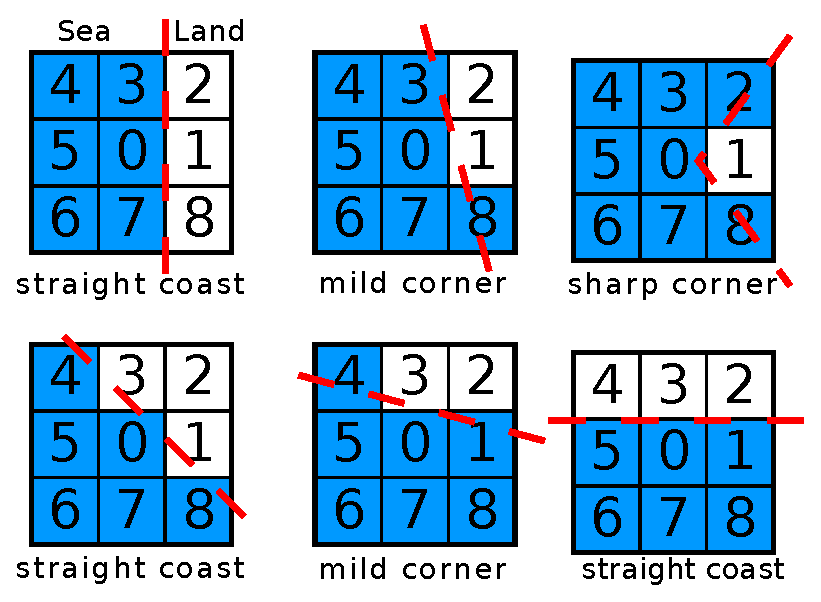
\epsfig{file=./num/coast_reflection.eps,angle=0,width=3in}
\caption{使用陆海掩膜确定岸线取向和几何的示例。对于任一海点（编号 0，蓝色海洋）且其至少有一个邻点为陆地（白色），使用编号为 1 到 8 的八个相邻点定义岸线几何。对于“平缓”拐角和笔直海岸，估计的岸线取向（虚线）用于计算反射波能的方向分布。}
\label{fig:refl} \botline
\end{center}
\end{figure}

为此，我们按图 \ref{fig:refl} 所示区分相对于局地点的三种岸线几何：对笔直海岸（相邻点中有三个连通陆点）设 $n=2$；对平缓拐角（相邻点中有两个陆点）设 $n=1$；对尖锐拐角（4 个最近相邻点中仅有一个陆点）设 $n=0$，这对应与子网格岛屿和冰山相同的处理。把这些 $n$ 值在 $0$ 到 $2$ 范围内改变，对结果影响很小。$n=1$ 对应 Lambert 面近似，该近似用于粗糙表面的电磁波散射。若 $n$ 为无穷大，则得到纯镜面反射。更严格的处理应使用海洋波长尺度上的岸线取向分布，即约 100~m 量级。

\vsssub
\subsubsection{~二阶谱和自由次重力波} \label{sec:IG1}
\vsssub

\opthead{IG1}{\ws}{F. Ardhuin}

\noindent 
警告：{\it 已发现非结构网格中 IG 波源存在一个错误。稍后将提供使用较旧代码版本的模式补丁。}

第 \ref{sec:intro} 节中使用的线性色散关系能很好近似大部分波能，但在高频谱区也存在不可忽略的部分，典型频率高于风海波峰频率的三倍 \citep[e.g.][]{rep:Lec13}。在浅水中，谱的另一种强非线性部分出现在很低频率处，称为次重力波。

在平底上水平均匀条件下，低频和高频非线性分量都可利用摄动理论由线性波谱估计 \citep[e.g.][]{art:Has62}。此外，均匀波场的非线性演变用这种“线性化谱”描述更为合适。因此，使用这种“线性化谱”工作，并在模式结果后处理时转换为包含非线性分量的可观测谱，是一种实用做法。执行该转换的一种方法是 \cite{art:Kra94} 提出的正则变换。该变换的性质由 \cite{art:Jan09} 进一步研究，并在 ECMWF 版本 WAM 模式中实现用于后处理。

P. Janssen 编写的正则变换代码已与 \ws\ 接口。使用 {\code IG1} 开关并在 {\F SIG1} namelist 中设置参数 {\code IGADDOUTP = 2} 时，该守恒能量的正则变换将用于输出点谱。如果 {\code IGADDOUTP = 1}，则按理论 \citep[e.g.][]{art:Has62} 在模式谱上叠加二阶谱。该选项不守恒能量，而且由于忽略了二阶谱中的准线性项，在高频处并不一致 \citep{art:Jan09}。

然而，与测量资料比较时，应注意不同观测装置对谱中非线性部分有不同响应。特别是，随波面运动的浮标也会把谱线性化，而二阶压力场与二阶表面高程之间并不满足线性波所用的关系。因此，正则变换只适用于在固定位置测量高程的波高仪。

当波场不均匀时，波浪的非线性性质会导致不同模态之间的能量交换。在浅水中，这通常导致能量向次重力波转移，这些波在岸线附近释放并作为自由波传播。{\code IG1} 开关允许用若干方法参数化该效应。与需要以很高空间分辨率求解破波带内双谱演变的完整水动力解相比，这些参数化非常粗略 \citep[e.g.][]{art:HB97}。默认 namelist 设置对应 \cite{art:Aea14} 提出的参数化，并在 6.06 版中做了小幅调整。$\widehat{E}_{IG}(f)$ 定义中的幂次从 $f^{1.5}$ 改为 $f^{1.0}$，相应常数从 0.015 调整为 0.013。

在实际中，自由次重力波能量通过 $S_{ref}$ 源项加入，即把 {\code SIG1} namelist 的 {\code IGSOURCE} 设为 1 或 2。

第一种方法由 {\code IGSOURCE =1} 激活，二阶谱可使用 Hasselmann 摄动（{\code IGMETHOD = 1}）或正则变换（{\code IGMETHOD} 的任何其他值）计算，如 \cite{art:Jan09} 所述。该方法可能得到更好的 IG 波能方向分布，但仍在测试中。第二种方法由 {\code IGSOURCE = 2} 激活，自由 IG 谱由以下表达式给出：

\begin{eqnarray}
 A_{IG} & =&    H_s T_{m0,-2}^2\label{eq:IGfit0}, \\
\widehat{E}_{IG}(f)& = & 1.2 \alpha_1^2 \frac{k g^2}{c_g 2 \pi f} \frac{(A_{IG}/4)^2}{\Delta_f}  
\left[\min( 1., 0.013\mathrm{Hz}/ f)\right]^{1.0}, \label{eq:IGfit1} \\
 \widehat{E}_{IG}(f,\theta) & = & \widehat{E}_{IG}(f) / (2 \pi ),
\label{eq:fit2} 
\end{eqnarray}

\noindent
其中平均周期定义为 $ T_{m0,-2} =\sqrt{m_{-2}/m_{0}}$，各阶矩为

\begin{equation}
 m_n= \int_{f_{min}~\mathrm{Hz}}^{0.5~\mathrm{Hz}} E(f) f^n {\mathrm d}f,\label{eq:mn}
\end{equation}

\noindent
经验系数 $\alpha_1$ 的量级为 $10^{-3}$~s$^{-1}$，由 {\code SIG1} namelist 参数 {\code IGEMPIRICAL} 设置。定义 $ T_{m0,-2}$ 所用的最小频率 $f_{min}$ 由 namelist 参数 {\code IGMAXFREQ} 设置；它也是施加该能量源的 IG 频带的最高频率。此外，在该频带内，可把海岸处的 IG 能量叠加到已有能量之上，也可把已有能量重置为零。后一种行为是默认设置，由 {\code IGBCOVERWRITE = 1} 控制。若选择其他设置（{\code IGBCOVERWRITE = 0}），结果对允许的最大岸线反射系数（{\F REF1} namelist 中的 {\code REFRMAX} 参数）非常敏感。

最后，也可在超过 $f_{min}$ 的频率上加入 IG 能量；这是默认行为，通过设置 {\code IGSWELLMAX = TRUE} 激活。对于 IG 波场的这一部分，IG 波源现在被减小 4 倍，该因子目前硬编码在 {\file w3ref1md.ftn} 中。它应与由 {\F REF1} namelist 参数 {\code REFRMAX} 定义的最大反射一起调整。在当前版本中，{\code IGSWELLMAX = TRUE} 选项在非结构网格上工作效果不好。因此建议这些网格使用 {\code IGSWELLMAX = FALSE}，但这会不幸地导致 IG 频带与涌浪-风海频带之间出现谱隙。





\vspace{\baselineskip}
\vssub
\subsection{~气海过程}
\vsssub
\subsubsection{~一般概念}
\vsssub

\ws\ 中还提供了一些附加子程序，用作耦合海洋-波浪或海洋-大气系统的一部分。这些子程序用于计算与表面波场有关、并准备传递给外部模式（例如海洋模式）的附加量。设置这些子程序的动机，是让外部模式能够包含波浪对风应力、上层海洋湍流等量的影响。

\paragraph{依赖海况的气海通量}

气海动量通量，或总风应力，是进入表面波和次表层流的动量通量之和。不考虑表面重力波场影响的耦合大气-海洋模式，通常根据风速与风应力之间的经验关系（通过阻力系数 $C_d$）计算总风应力。所提供的 {\it FLD} 子程序允许基于 \ws\ 波数-方向谱计算总风应力，供耦合数值模式使用。

在一阶近似下，总风应力等于进入表面波的动量通量（表面波形状阻力）与直接进入次表层流的动量通量（通过黏性应力）之和。进入波浪的动量通量可表示为波方差谱乘以波增长率（动量吸收率）的积分。计算波形状阻力需要若干假设。首先，波形状阻力在一阶上对高频波（或谱尾）的水平敏感。波谱的这一部分在波浪模式中有很大不确定性，因此在计算风应力时可能需要单独参数化。因此，必须假定一种方式来参数化高频部分；在风速超过 15 m/s 时，该部分不受观测资料约束。其次，需要对波增长率函数作出假设，因为历史上它通常由风速或风应力来参数化。无论哪种情况，增长率函数都需要基于波长以及波向相对于风和/或应力方向的经验系数。第三，波形状阻力会对波边界层（大致为气海界面以上 10 m 内）的湍流剖面和风剖面产生反馈。这种反馈在决定风应力和平均风剖面方面究竟有多重要，目前尚未完全理解。最后，已知破碎波与非破碎波上的增长率不同。然而，目前没有简单方法能在风应力计算模型中显式包含破碎波影响。因此，当前两个 {\it FLD} 子程序均不区分破碎波和非破碎波的增长率。

总气海动量通量可（一阶近似）表示为：
\begin{equation}
\vec{\tau}=\vec{\tau}_{\nu}+\vec{\tau}_{f},
\end{equation}
其中 $\vec{\tau}_{\nu}$ 为黏性应力矢量，$\vec{\tau}_{f}$ 为波形状阻力。在气海界面处，波形状阻力可作为进入所有波浪的动量通量贡献计算：
\begin{equation}\label{formdrag}
\vec{\tau}_{f}=\rho_w\int_{k_{min}}^{k_{max}}\int_{-\pi}^{\pi} \beta_g(k,\theta) \sigma F (k,\theta) d\theta \vec{k} dk,
\end{equation}
其中 $\rho_w$ 为水密度，$k$ 为波数，$\theta$ 为波向，$\sigma$ 为角频率，$\beta_g (k,\theta)$ 为增长率，$F (k,\theta)$ 为波方差谱，$k_{min}$ 和 $k_{max}$ 为产生贡献的波的最小和最大波数。增长率表达式取决于模式所采用的理论，并将在各理论的说明中分别描述。

风速超过 15 m/s 时，谱尾在观测和理论上约束都不足。因此，{\it FLD} 子程序中的谱尾水平以经验方式参数化，使平均阻力系数对应于建模系统中使用的标准整体阻力系数。这样，使用任何显式依赖海况的风应力公式都不会改变风应力的平均值，但应力会根据海况偏离该平均值。这里假定谱尾水平仅是风速的函数，与海况无关。

\vsssub
\subsubsection{~依赖海况的 $\tau$：Reichl et al. 2014} \label{sec:FLD1}
\vsssub

\opthead{FLD1}{\ws}{B. Reichl}

\paragraph{Reichl et al., 2014 的风应力}

在 \citet{art:Rei14} 中，总应力随高度保持常数，但按高度分解为两个分量：
\begin{equation}
\vec{\tau}=\vec{\tau}_t(z)+\vec{\tau}_f(z),
\end{equation}
其中 $\tau_t$ 为湍流应力，在非常接近海面的地方等于黏性应力。波形状应力可表示为：
\begin{equation}
\vec{\tau}_f(z)=\rho_w\int^{k=\delta/z}_{k_{min}} \int^\pi_{-\pi}\beta_g(k,\theta) \sigma F(k,\theta) d\theta {\vec{k}} dk,
\end{equation}
也就是说，高度 $z$ 处的波形状应力等于对海面处波形状应力在低于 $k=\delta/z$ 的波数范围内积分，其中 $\delta/k$ 是波数为 $k$ 的波对应的内层高度 \citep{art:Har04}。该表达式由如下假设推导而来：波致应力从海面到内层高度范围内显著，而在更高处可忽略。由于在海面处
\begin{equation}
\vec{\tau}=\vec{\tau}_\nu+\vec{\tau}_f(z=0)=\vec{\tau}_\nu+\rho_w\int^{k_{max}}_{k_{min}} \int^\pi_{-\pi}\beta_g(k,\theta) \sigma F(k,\theta) d\theta {\vec{k}} dk,
\end{equation}
高度 $z$ 处的湍流应力可表示为：
\begin{equation}
\vec{\tau}_t(z)=\vec{\tau}_\nu+\rho_w\int^{k_{max}}_{k=\delta/z} \int^\pi_{-\pi}\beta_g(k,\theta) \sigma F(k,\theta) d\theta {\vec{k}} dk.
\end{equation}

在该模型中，假定内层高度 $z=\delta/k$ 处的湍流应力决定波数为 $k$ 的波的增长率：
\begin{equation}
\beta_g(k,\theta)=c_\beta \sigma\frac{\left|\tau_t(z=\delta/k)\right|}{\rho_wc^2}\cos^2(\theta-\theta_\tau),
\end{equation}
其中 $\theta_\tau$ 是内层高度处湍流应力的方向。使用内层高度处的湍流应力代替总风应力，是因为较长波会削弱较短波受到的有效风强迫（波浪遮蔽）。

增长率系数 $c_\beta$ 随波相速与局地湍流摩擦速度（内层高度处的摩擦速度）之比而变化，$u_\star^l=\sqrt{\tau_t(z=\delta/k)/\rho_a)}$。
\begin{equation}
c_{\beta}=\left\{
\begin{array}{cll} 
25  &: \cos(\theta-\theta_w)>0 \hspace{2mm}&:c/u_{\star}^l<10\\
10+15\cos[\pi(c/u_\star-10)/15]   &:&:10\le c/u_{\star}^l<25 \\
-5  &:&:25\le c/u_{\star}^l\\
-25  &: \cos(\theta-\theta_w)<0 &\\
\end{array}
\right.
\end{equation}

风廓线在波边界层中利用能量守恒约束显式计算。从黏性子层顶部到最短波的内层高度，风切变表示为：
\begin{equation}
\frac{d {\vec{u}}}{\partial z}=\frac{\rho_a}{\kappa z}\left|\frac{ \vec{\tau}_\nu}{\rho_a}\right|^{3/2}\frac{\vec{\tau}_\nu}{\vec{\tau}_\nu\cdot\vec{\tau}_{tot}}\hspace{3mm}{\rm for}\hspace{3mm}z_\nu<z<\delta/k_l.
\end{equation}
在最短波的内层高度与最长波的内层高度之间，风切变表示为：
\begin{equation}
\frac{d {\vec{u}}}{\partial z}=\left[ \frac{\delta}{z^2}\tilde{F}_w\left(k=\frac{\delta}{z}\right)+\frac{\rho_a}{\kappa z}\left| \frac{\vec{\tau}_t(z)}{\rho_a}\right|^{3/2} \right]\times\frac{\vec{\tau}_t(z)}{\vec{\tau}_t(z)\cdot\vec{\tau}_{tot}}\hspace{3mm}{\rm for}\hspace{3mm}\delta/k_l\le z,
\end{equation}
其中 $\tilde{F}_w(k=\delta/z)$ 是表面波吸收的能量：
\begin{equation}
\tilde{F}_w(k=\delta/z)=\rho_w\int^{\pi}_{-\pi}\beta_g(k,\theta)gF(k,\theta)k d\theta.
\end{equation}
最后，在最长波的内层高度以上，波浪影响可忽略，风切变沿风应力方向排列：
\begin{equation}
\frac{d{\vec{u}}}{dz}=\frac{u_\star}{\kappa z}\frac{\vec{\tau}_{tot}}{|\vec{\tau}_{tot}|}.
\end{equation}

注意，使用 FLD1 开关时，黏性应力、摩擦速度、表面粗糙长度和 Charnock 参数的内部变量和输出值会被重新计算并覆盖。

\vsssub
\subsubsection{~依赖海况的 $\tau$：Donelan et al. 2012} \label{sec:FLD2}
\vsssub

\opthead{FLD2}{UMWM}{B. Reichl}

\paragraph{Donelan et al., 2012 的风应力}
在 \citet{art:Don12} 中，式 (\ref{formdrag}) 中的增长率参数表示为：
\begin{equation}
\beta_g(k,\theta)=A_1 \sigma \frac{\left[u_{\lambda/2} \cos(\theta-\theta_w)-c\right]\left| u_{\lambda/2}cos(\theta-\theta_w)-c \right|}{c^2}\frac{\rho_a}{\rho_w},
\end{equation}
\begin{equation}
A_{1}=\left\{
\begin{array}{lll} 
0.11, & :  u_{\lambda/2}\cos\theta>c,  &\mbox{for wind forced sea}\\
0.01 & :   0<u_{\lambda/2}\cos\theta<c, &\mbox{for swell faster than the wind}\\
0.1 & :  \cos\theta<0,  &\mbox{for swell opposing the wind}
\end{array}
\right.
\end{equation}
其中 $A_1$ 为经验确定的比例系数（使模拟波谱与现场观测一致），$u_{\lambda/2}$ 为半波长高度处的风速（最高取到 20 m），$\theta_w$ 为风向，$c$ 为波相速。风速使用粗糙表面的壁面律计算：
\begin{equation}
u(z)=\frac{u_\star}{\kappa}\ln\left(\frac{z}{z_0}\right),
\end{equation}
其中 $\kappa$ 为 von K\'arm\'an 系数（默认 0.4）。黏性应力由光滑表面的壁面律计算。黏性阻力系数 $Cd_\nu$ 会调整以考虑遮蔽作用：
\begin{equation}
Cd'_\nu=\frac{Cd_\nu}{3}\left(1+\frac{2 Cd_\nu}{Cd_\nu+Cd_f}\right),
\end{equation}
其中 $Cd_f$ 为波形状阻力系数。于是黏性应力可解为：
\begin{equation}
\vec{\tau}_\nu=\rho_a Cd'_\nu \left|{\bf u_{z}}\right|{\bf {u}}_{z}.
\end{equation}

注意，使用 FLD2 开关时，黏性应力、摩擦速度、表面粗糙长度和 Charnock 参数的内部变量和输出值会被重新计算并覆盖。

\vspace{\baselineskip}
\vssub
\subsection{~输出参数} \label{sub:outpars}
\vssub

波浪模式可在模式地理网格上输出参数；这些参数可以是积分参数，也可以是频率函数，此时每个频率对应一个网格。所有作为频率函数的参数（例如 \textbf{EF} 或 \textbf{USF}）都需要在 ww3\_grid.inp 或 ww3\_grid.nml 中定义的 {\F OUTS} namelist 中设置特定 namelist 参数。这样做是为了在不需要这些参数时减少内存使用。

下面给出输出场参数的简要定义。定义表可在 \para\ref{sec:ww3shel} 的示例 {\code ww3\_shel.inp} 文件中找到。该输入文件还提供了一组标志，用于指示不同场输出文件类型（ASCII、grib、igrads、NetCDF）是否支持相应输出参数。若需了解这些参数如何计算，用户可阅读 {\code w3iogomd.F90} 模块中 {\code w3iogo} 例程的代码。

在 {\code ww3\_shel.nml} 或 {\code ww3\_shel.inp} 中选择场输出，最简单的方法是给出所需参数列表。例如，{\textbf HS DIR SPR} 会要求计算有效波高、平均方向和方向扩展。它们随后会存储在 {\code out\_grd.XX} 文件中，并可进行后处理，例如使用 {\code ww3\_ouf} 转为 NetCDF。示例见 \para\ref{sec:ww3multi} 和 \para\ref{sec:ww3ounf}。这些 namelist 使用下列粗体名称，例如 \textbf{HS}。

下面列出的所有参数都可在 ASCII 和 NetCDF 输出文件中使用。如果选择的输出文件类型为 grads 或 grib，部分参数可能不可用。是否可用由 \para\ref{sec:ww3shel} 示例输入文件中场输出参数表的前两列标识。该表还为所有参数列出内部 WAVEWATCH III 代码标签、输出标签（ASCII 文件扩展名、NetCDF 变量名和基于 namelist 的选择所用名称，另见 \para\ref{sec:ww3ounf}），以及较长的参数名称/定义。

当结果对未解析谱段（$f<f_{NK}$）贡献不太敏感时，谱尾贡献按谱的幂律衰减进行参数化，默认 $E(f,\theta) = E(f_{NK},\theta) (f_{NK}/f)^{-5}$。对某些参数而言，这样做要么不必要，要么可能造成误导，因此积分仅计算到 $f_{NK}$。


最后需注意，在所有定义中，频率均为\emph{相对}频率。因此，在有流存在时，这些参数只能与漂流测量资料，或以波数获得后转换为频率的数据进行比较。若要与固定仪器资料比较，需要使用完整谱并正确转换到固定参考系。

\begin{list}{\Roman{outgrps})\hfill}
            {\usecounter{outgrps} \leftmargin 7mm \labelwidth 5mm
             \rightmargin 0mm \itemsep \baselineskip \parsep 0mm}

\item {强迫场}

\begin{list}{\arabic{outpars})\hfill}
            {\usecounter{outpars} \leftmargin 8mm \labelwidth 7mm
             \rightmargin 0mm \itemsep 0mm \parsep 0mm}
\item \textbf{DPT} 平均水深 (m)。包括变化水位。
\item \textbf{CUR} 平均流速（矢量，m/s）。
\item \textbf{WND} 平均风速（矢量，m/s）。该风速始终为输入模式的风速，即未针对流速修正。
\item \textbf{AST} 气海温差 ($^\circ$C)。
\item \textbf{WLV} 水位。
\item \textbf{ICE} 冰密集度。
\item \textbf{IBG} 冰山导致的波浪衰减：该参数是在小冰山场中与波能损失相关的 e 折尺度的倒数 \citep{art:Aea11}。
\item \textbf{D50} 沉积物中值粒径 ($D_{50}$)。
\item \textbf{IC1} 冰厚。
\item \textbf{IC5} 最大浮冰直径，$D_{\max}$。
\end{list}

\item{标准平均波浪参数}

\begin{list}{\arabic{outpars})\hfill}
            {\usecounter{outpars} \leftmargin 8mm \labelwidth 7mm
             \rightmargin 0mm \itemsep 0mm \parsep 0mm}
\item \textbf{HS} 有效波高 (m) [见式~(\ref{eq:etot})]
      \begin{equation} H_s = 4 \sqrt{E} \: . \label{eq:Hs} \end{equation}
\item \textbf{LM} 平均波长 (m) [见式~(\ref{eq:zbar})]
      \begin{equation} L_m = 2\pi \overline{k^{-1}}
      \: . \label{eq:Lm} \end{equation}
\item \textbf{T02} 平均波周期 (s) [见式~(\ref{eq:zbar})]
      \begin{equation} T_{m02} = 2\pi /\sqrt{\overline{\sigma^{2}}}
      \: . \label{eq:Tm02} \end{equation}
\item \textbf{T0M1} 平均波周期 (s) [见式~(\ref{eq:zbar})]
      \begin{equation} T_{m0,-1} = 2\pi \overline{\sigma^{-1}}
      \: . \label{eq:Tm0m1} \end{equation}
\item \textbf{T01} 平均波周期 (s) [见式~(\ref{eq:zbar})]
      \begin{equation} T_{m0,1} = 2\pi /\overline{\sigma}
      \: . \label{eq:Tm} \end{equation}
\item \textbf{FP} 峰值频率 (Hz)，由一维频率谱在离散峰附近作抛物线拟合计算。
\item \textbf{DIR} 平均波向（度，气象约定）
      \begin{equation} \theta_m = \mbox{atan} \left ( \frac{b}{a} \right )
      \: , \label{eq:theta_m} \end{equation} \begin{equation}
      a = \int_0^{2\pi} \int_0^\infty \cos(\theta) F(\sigma,\theta) \:
      d\sigma \: d\theta \: , \end{equation} \begin{equation}
      b = \int_0^{2\pi} \int_0^\infty \sin(\theta) F(\sigma,\theta) \:
      d\sigma \: d\theta \: . \end{equation}
\item \textbf{SPR} 平均方向扩展 \citep[度；][]{art:KVH88}
      \begin{equation} \sigma_\theta = \left [ 2 \left \{ 1 - \left (
      \frac{a^2+b^2}{E^2} \right )^{1/2} \right \} \right ]^{1/2}
      \: , \label{eq:sig_th} \end{equation}
\item \textbf{DP} 峰值方向（度），定义方式与平均方向相同，但只使用包含峰值频率的谱 $F(k)$ 的频率/波数箱。
\item \textbf{HIG} 次重力波高度。
\item \textbf{MXE} 最大海面高程（时空极值，STE）
\item \textbf{MXES} 最大海面高程标准差（STE）
\item \textbf{MXH} 最大波高（STE）
\item \textbf{MXHC} 由波峰得到的最大波高（STE）
\item \textbf{SDMH} MXC 的标准差（STE）
\item \textbf{SDMHC} MXHC 的标准差（STE）
\item \textbf{WBT} 主导波浪破碎概率 $b_T$ (\ref{eq:bt})
\item \textbf{TP} 峰值波周期，由峰值频率（\textbf{FP}）的倒数得到。
\end{list}

\item{谱参数（前 5 个矩和波数）。

所有这些参数都是频率的函数，因此为三维数组。由于内存占用较大，计算这些参数需要在 {\F OUTS} namelist 中激活相应开关。}

\begin{list}{\arabic{outpars})\hfill}
            {\usecounter{outpars} \leftmargin 8mm \labelwidth 7mm
             \rightmargin 0mm \itemsep 0mm \parsep 0mm}
   
\item \textbf{EF} 波浪频率谱 (m$^2$/Hz)
      \begin{equation} E(f) = 2 \pi  \int F(\sigma,\theta) \mathrm{d} \theta 
      \: . \label{eq:Ef} \end{equation}
\item \textbf{TH1M} 每个频率的平均方向 \citep[度；][]{art:KVH88}
       \begin{equation} \theta_1 (f)= \mbox{atan} \left ( \frac{b_1(f)}{a_1(f)} \right )
      \: , \label{eq:theta_b} \end{equation} \begin{equation}
      a_1(f) = 2 \pi \int_0^{2\pi} \int_0^\infty \cos(\theta) F(\sigma,\theta) \:
       \mathrm{d}\theta \: , \end{equation} \begin{equation}
      b_1(f) = 2 \pi \int_0^{2\pi} \int_0^\infty \sin(\theta) F(\sigma,\theta) \:
       \mathrm{d}\theta \: . \end{equation}
\item \textbf{STH1M} 每个频率的第一方向扩展（度；）
      \begin{equation} \sigma_1(f) = \left [ 2 \left \{ 1 - \left (
      \frac{a_1(f)^2+b_1(f)^2}{E(f)^2} \right )^{1/2} \right \} \right ]^{1/2}
      \: , \label{eq:sig_th1} \end{equation}
\item \textbf{TH2M} 由 $a_2$ 和 $b_2$ 得到的平均方向（度）
       \begin{equation} \theta_2 (f)= 0.5 \mbox{atan} \left ( \frac{b_2(f)}{a_2(f)} \right )
      \: , \label{eq:theta_2} \end{equation} \begin{equation}
      a_2(f) = 2 \pi \int_0^{2\pi} \int_0^\infty \cos(2 \theta) F(\sigma,\theta) \:
       \mathrm{d}\theta \: , \end{equation} \begin{equation}
      b_2(f) = 2 \pi \int_0^{2\pi} \int_0^\infty \sin(2 \theta) F(\sigma,\theta) \:
       \mathrm{d}\theta \: . \end{equation}
\item \textbf{STH2M} 由 $a_2$ 和 $b_2$ 得到的方向扩展（度）
      \begin{equation} \sigma_2(f) = \left [ 0.5 \left \{ 1 - \left (
      \frac{a_2(f)^2+b_2(f)^2}{E(f)^2} \right )^{1/2} \right \} \right ]^{1/2}
      \: , \label{eq:sig_th1} \end{equation}
\item \textbf{WN} 波数 $k(\sigma)$ (rad/m)
      \begin{equation} \sigma^2 = g k \tanh (k D) 
      \: , \label{eq:k} \end{equation}
\end{list}

\item{谱分区参数} \label{out:spec_part}

这些输出参数基于把谱划分为各个独立波场。

\begin{list}{\arabic{outpars})\hfill}
            {\usecounter{outpars} \leftmargin 8mm \labelwidth 7mm
             \rightmargin 5mm \itemsep 0mm \parsep 0mm}


\item \textbf{PHS} 谱分区的波高 $H_s$（见下文）。\label{out:first_part}
\item \textbf{PTP} 谱分区的峰值（相对）周期（抛物线拟合）。
\item \textbf{PLP} 谱分区的峰值波长（由峰值周期得到）。
\item \textbf{PSP} 谱分区的平均方向。
\item 谱分区的方向扩展，参见式~(\ref{eq:sig_th})。
\item \textbf{PWS} 谱分区的风海比例。采用 \cite{art:HP01} 的方法，并按 \cite{tol:Oahu07a} 所述实现。由此引入“风海比例” $W$：
\begin{equation}
W = E^{-1}  \: E |_{U_p > c}  \:\:\: , \label{eq:wsf}
\end{equation}
其中 $E$ 为总谱能，$E |_{U_p > c}$ 是谱中投影风速 $U_p$ 大于局地波相速 $c = \sigma / k$ 的区域内的能量。后者定义了谱中受风直接影响的区域。为允许非线性相互作用把该边界移向较低频率，并随后在该区域内形成充分成长的风海，$U_p$ 包含一个乘子 $C_{mult}$：
\begin{equation}
U_p = C_{mult} U_{10} \cos ( \theta - \theta_w )  \:\:\: . \label{eq:Up}
\end{equation}
该乘子可由用户设置，默认值为 $C_{mult} = 1.7$。
\item \textbf{PDP} 谱分区的峰值方向。
\item \textbf{PQP} 谱分区的 Goda 峰度。
\item \textbf{PPE} 谱分区的 JONSWAP 峰值增强因子。它度量相对于对应 \citeauthor{art:PM64} 谱峰值的谱峰放大。
\item \textbf{PGW} 谱分区的 Gaussian 频率宽度 (Hz)。即把 Gaussian 谱最小二乘拟合到一维谱分区。
\item \textbf{PSW} 谱分区的谱宽 \citep{art:LH84}
\item \textbf{PTE} 谱分区的波能周期 [见式~(\ref{eq:Tm0m1})]
\item \textbf{PT1} 谱分区的平均波周期 [见式~(\ref{eq:Tm})]
\item \textbf{PT2} 谱分区的波浪零上跨周期 [见式~(\ref{eq:Tm02})]
\item \textbf{PEP} 谱分区的波浪峰值谱密度
\item \textbf{TWS} 整个谱的风海比例。
\item \textbf{PNR} 在谱中找到的分区数量。\label{out:last_part}
\end{list}


\item{大气-波浪层}
\begin{list}{\arabic{outpars})\hfill}
            {\usecounter{outpars} \leftmargin 8mm \labelwidth 7mm
             \rightmargin 0mm \itemsep 0mm \parsep 0mm}
\item \textbf{UST} 摩擦速度 $u_\ast$（标量）。定义取决于所选源项参数化 (m/s)。应力的另一种矢量版本可用于研究（需要用户修改代码）。
\item \textbf{CHA} 气海摩擦的 Charnock 参数（无量纲）
\item \textbf{CGE} 能量通量 (W/m)
      \begin{equation} C_g E =  \rho_w g \overline{C_g} E
      \: . \label{eq:CgE} \end{equation}
\item \textbf{FAW} 风到波浪的能量通量
\item \textbf{TAW} 净波浪支撑应力（风到波浪的动量通量）
\item \textbf{TWA} 波浪支撑应力的负值部分
\item \textbf{WCC} 白冠覆盖率（无量纲）
\item \textbf{WCF} 波浪到风的动量通量
\item \textbf{WCH} 白冠平均厚度 (m)
\item \textbf{WCM} 平均破碎波高 (m)（尚不可用）
%\item \textbf{PWS} Moment of whitecap distribution (?) (NOT PLUGGED YET)
\end{list}

\item{波浪-海洋层}

\begin{list}{\arabic{outpars})\hfill}
            {\usecounter{outpars} \leftmargin 8mm \labelwidth 7mm
             \rightmargin 0mm \itemsep 0mm \parsep 0mm}
\item \textbf{SXY} 辐射应力
      \begin{equation} S_{xx} = \rho_w g \int \!\!\!\! \int \left
        ( n - 0.5 + n \cos^2 \theta \right )  \: F(k,\theta) \: dk d\theta
      \: , \label{eq:Sxx} \end{equation}
      \begin{equation} S_{xy} =\rho_w g \int \!\!\!\! \int
        n \sin \theta \cos \theta  \: F(k,\theta) \: dk d\theta
      \: , \label{eq:Syy} \end{equation}
      \begin{equation} S_{yy} =\rho_w g \int \!\!\!\! \int \left
        ( n - 0.5 + n \sin^2 \theta \right )  \: F(k,\theta) \: dk d\theta
      \: , \label{eq:Sxy} \end{equation}
      其中
      \begin{equation} n = \frac{1}{2} + \frac{kd}{\sinh 2kd}
      \: . \label{eq:n} \end{equation}
\item \textbf{TWO} 波浪到海洋的动量通量 (m$^2$/s$^2$)
\item \textbf{BHD} Bernoulli 水头 (m$^2$/s$^2$)
      \begin{equation} J =  g \int \!\!\!\! \int  \frac{k}
        {\sinh 2kd}  \: F(k,\theta) \: dk d\theta
      \: , \label{eq:BHD} \end{equation}
\item \textbf{FOC} 波浪到海洋的能量通量 (W/m$^2$)
\item \textbf{TUS} Stokes 体积输运 (m$^2$/s)
     \begin{equation} (M^w_x,M^w_y) =  g \int \!\!\!\! \int  \frac{(k \cos(\theta),k \sin(\theta))}
        {\sigma}  \: F(k,\theta) \: dk d\theta
      \: , \label{eq:Mw} \end{equation}
\item \textbf{USS} 海表 Stokes 漂流 (m/s)
     \begin{equation} (U_{ssx},U_{ssy}) =  \int \!\!\!\! \int  \sigma \cosh 2kd \frac{(k \cos(\theta),k \sin(\theta))}
        {\sinh^2 kd}  \: F(k,\theta) \: dk d\theta
      \: , \label{eq:Uss} \end{equation}
\item \textbf{P2S} 二阶压力方差 (m$^2$) 以及该压力的峰值周期 (s)，它们会对声学和地震噪声产生贡献：
      \begin{equation} F_{p2D}(k=0) = \int_0^{\infty} \frac{4 \sigma}{C_g} \int_0^{\pi}  F(k,\theta) \:  F(k,\theta+\pi) \:  d\theta dk
      \: , \label{eq:sop} \end{equation}
\item \textbf{USF} 海表 Stokes 漂流的频率谱 (m/s/Hz)
     \begin{equation} (U_{ssx}(f),U_{ssy}(f)) =  \int \sigma \cosh 2kd \frac{(k \cos(\theta),k \sin(\theta))}
        {\sinh^2 kd}  \: F(k,\theta) \frac{2 \pi}{C_g} d\theta
      \: , \label{eq:Ussf} \end{equation}
注意，为激活 USF 输出所需的三维数组，必须在 ww3\_grid.inp 的 OUTS namelist 中设置 US3D=1。
\item \textbf{P2L} 二阶压力的频率谱 (m$^2$s)，它对声学和地震噪声有贡献：
      \begin{equation} F_{p2D}(k=0,f) =  \frac{2 \sigma}{\pi} \int_0^{\pi}  \frac{4 \pi^2}{C_g^2} F(k,\theta) \:  F(k,\theta+\pi) \:  d\theta
      \: . \label{eq:sopf} \end{equation}
\item \textbf{TWI} 波浪到海冰的应力
\item \textbf{FIC} 波浪到海冰的能量通量
\item \textbf{USP} 按运行时定义的频率分量划分的表层 Stokes 漂流 (m/s)：
      \begin{equation} (U_{ssp},V_{ssp})(n) =  \int \!\!\!\! \int_{k_n}  \sigma \cosh 2kd \frac{(k\
      \cos(\theta),k \sin(\theta))}
        {\sinh^2 kd}  \: F(k,\theta) \: dk d\theta
      \: . \label{eq:Ussp} \end{equation}
这里的数量 $n$ 以及各分区中心波数 $k_n$ 称为“运行时”量，因为它们定义在由 ww3\_grid.inp 生成的模式定义文件中（这些量的设置细节见示例输入文件）。每个 $n$ 分区的波数积分边界会划分模式波谱，以适应给定的 $k_n$ 值。
\item \textbf{TOC} 总海洋应力 (Pa)
      \begin{equation} \tau_{oc} = \tau_a - \tau_{aw} + \tau_{woc}
      \: . \label{eq:Toc} \end{equation}
\end{list}

\item{波浪-海底层}

\begin{list}{\arabic{outpars})\hfill}
            {\usecounter{outpars} \leftmargin 8mm \labelwidth 7mm
             \rightmargin 0mm \itemsep 0mm \parsep 0mm}

\item \textbf{ABR} 近底均方根位移幅度
      \begin{equation} a_{b,rms} = \left [ 2 \int \!\!\!\! \int
      \frac{1}{\sinh^2 kd} \: F(k,\theta) \: dk d\theta \right ] ^{1/2}
      \: . \label{eq:ab_rms} \end{equation}
\item \textbf{UBR} 近底均方根轨道速度
      \begin{equation} u_{b,rms} = \left [ 2 \int \!\!\!\! \int
      \frac{\sigma^2}{\sinh^2 kd} \: F(k,\theta) \: dk d\theta \right ] ^{1/2}
      \: . \label{eq:ub_rms} \end{equation}
\item \textbf{BED} 床形参数：沙纹高度和方向（尚未测试）
\item \textbf{FBB} WBBL 中的能量耗散
\item \textbf{TBB} WBBL 中的动量损失
\end{list}

\item{谱参数}

\begin{list}{\arabic{outpars})\hfill}
            {\usecounter{outpars} \leftmargin 8mm \labelwidth 7mm
             \rightmargin 0mm \itemsep 0mm \parsep 0mm}

\item \textbf{MSS} $u$ 和 $c$ 方向上的均方坡度（顺波和横波坡度方差分量）。
\item \textbf{MSC} 谱尾水平（无量纲）
\item \textbf{MSD} 最大坡度方差 mss$_u$ 的方向
\item \textbf{MCD} 谱尾方向
\item \textbf{QP} 峰度参数 \citep{art:G70}
      \begin{equation} Q_p = \frac{2}{E^2} \int_0^{f_{NK}} f \left( \int_0^{2\pi} 
      F(f,\theta) \:\rd \theta \right)^2 \: \rd  f \: \label{eq:qp}
      \end{equation}
\item \textbf{QKK} 波数峰度 \citep{art:DC23}
      \begin{equation} Q_{kk} = \frac{1}{E^2} \int_0^{f_{NK}} \int_0^{2\pi} 
      0.5 \left[ A(k,\theta)+ A(k,\theta+\pi)\right]^2 \frac{\sigma^2}{k C_g} \:\rd \theta  \: \rd  \sigma \: \label{eq:qkk}
      \end{equation}
\item \textbf{SKW} 在零坡度处采样的海面高程偏度。这是 \cite{Barrick&Lipa1985} 中定义的 $\lambda_1$ 参数，或 \cite{Srokosz1986} 中的 $\lambda_{3,0,0}$。它由表面高程的二阶修正计算，使用 P. Janssen 的 ECWAM 代码。
\item \textbf{EMB} 该量为 $-\gamma/8 = -(\lambda_{1,2,0}+\lambda_{1,0,2}-2 \lambda{0,1,1} \lambda{1,1,1})/8 (1-\lambda_{0,1,1}^2)$，使零坡度点的平均海面为 EMB$\times H_s$。
\item \textbf{EMC} 这是额外的跟踪器偏差系数，等于 $-\lambda_{3,0,0}/24$，它与 retracker 的选择有关，见 \cite{DeCarlo&Ardhuin2024} 中的 $J_z$ 函数。
\end{list}

\item{数值诊断}

\begin{list}{\arabic{outpars})\hfill}
            {\usecounter{outpars} \leftmargin 8mm \labelwidth 7mm
             \rightmargin 0mm \itemsep 0mm \parsep 0mm}
\item \textbf{DTD} 源项积分中的平均时间步长 (s)。
\item \textbf{FC} 截止频率 $f_c$ (Hz，取决于输入和耗散的参数化)。
\item \textbf{CFX} 空间平流的最大 CFL 数
\item \textbf{CFD} 角向平流的最大 CFL 数
\item \textbf{CFK} 波数平流的最大 CFL 数
\end{list}

\item{用户定义}

\begin{list}{\arabic{outpars})\hfill}
            {\usecounter{outpars} \leftmargin 8mm \labelwidth 7mm
             \rightmargin 0mm \itemsep 0mm \parsep 0mm}

\item \textbf{U1} 用户定义参数槽位（需要修改代码）。
\item \textbf{U2} 同上。
\end{list}

\end{list}




%\vspace{\baselineskip}
%\centerline{\ldots NEEDS CLEAN UP BELOW HERE \ldots}
%\vspace{\baselineskip}

%THESE TWO PARAMETERS WILL BE PUT BACK. 
%Old output types \ref{out:old_fpw} and \ref{out:old_thw} have become obsolete
%with the introduction of the partitioned output types \ref{out:first_part}
%through \ref{out:last_part}. However, they are retained in the present model
%release to provide required downward compatibility with model version 1.18 at
%NCEP. These output types are likely to be retired in upcoming versions of \ws.

\vssub
\subsection{~派生参数} \label{sub:outpars}
\vssub

\subsubsection{方向坡度和近天底后向散射}
在线性波假设下，海面坡度服从 Gaussian 分布，并由均方坡度张量 mss$_x$、mss$_y$、mss$_{xy}$ 完全描述。在 \ws\ 中，计算得到的 mss 参数包括顺波方向的 $\mathrm{mss}_u$，其方向由 $\mathrm{mss}_d$ 给出；以及垂直方向上的横波 $\mathrm{mss}_c$。

因此，在把 $\mathrm{mss}_d$ 转为弧度后，波浪模式解析的（长）波的均方坡度张量为
\begin{eqnarray}
   \mathrm{mss}_{x,\mathrm{long}} &=& \mathrm{mss}_u \cos^2(\mathrm{mss}_d)+\mathrm{mss}_c \sin^2(\mathrm{mss}_d) \\
   \mathrm{mss}_{y,\mathrm{long}} &=& \mathrm{mss}_u \sin^2(\mathrm{mss}_d)+\mathrm{mss}_c \cos^2(\mathrm{mss}_d) \\
   \mathrm{mss}_{xy,\mathrm{long}}&=&0.5 (\mathrm{mss}_u - \mathrm{mss}_c) \sin(2 \mathrm{mss}_d)
\end{eqnarray}
若要与近天底光学或雷达数据（高度计、GPM 或 CFOSAT/SWIM 数据）的后向散射功率（$\sigma^0$）等观测进行比较，应在这些量上加入短波（高于模式最高频率）的贡献。
   
\subsubsection{Stokes 漂流剖面}
海表 Stokes 漂流谱有两个分量，其计算为 \\
{\code usf(IK)= SUM( E(IK,ITH)*ECOS(ITH)*DTH(ITH) )*DK(IK)*2*WN(IK,ISEA) *  FACT(KD)/DF(IK)}

{\code vsf(IK)= SUM( E(IK,ITH)*ESIN(ITH)*DTH(ITH) )*DK(IK)*2*WN(IK,ISEA) *  FACT(KD)/DF(IK)}

其中 WN 为波数，FACT(KD) 为无量纲水深的函数。

由该谱可得到任意深度 $z$ 处的 Stokes 漂流，$z$ 由参考面 $z=0$ 起向上为正：

Us(z)= SUM{IK=I1,I2} ( usf(IK) * FACT2(z,KD)*DF(IK))
Vs(z)= SUM{IK=I1,I2} ( vsf(IK) * FACT2(z,KD)*DF(IK))

这需要知道局地水深 D、平均海面 LEV 以及波数 WN(IK)。因此 KD=D*WN(IK) 是频率/波数索引 IK 的局地函数。

系数 FACT2(z,KD) 在 KD $>$ 6 时等于 EXP(2*WN(IK)*(z-LEV))，否则为\\
FACT2(z,KD)=COSH(2*WN(IK)*(z+H))/COSH(2*WN(IK)*D).


\bpage

\section{~数值方法} \label{chapt:num}
\newcounters

% 本章正文正按 \input 文件逐节替换为中文。
Cartesian 坐标（\ref{eq:bal_plane}）或球坐标（\ref{eq:bal_sphere}）中的波作用量方程，是波浪模式的基本方程。不过，模式中使用的是这些方程的修正形式，其中：(a) 方程在可变波数网格上求解（见下文）；(b) 在选定数值格式中使用方程的修正形式，以正确描述离散方程的色散（见 \para\ref{sub:xy_prop}）；(c) 考虑岛屿等子网格障碍物（见 \para\ref{sub:xy_prop}）。


\vssub
\subsection{~谱离散} \label{sec:basic_num}
\vsssub


如果直接求解式 (\ref{eq:bal_plane}) 或式 (\ref{eq:bal_sphere})，在浅水中会出现有效谱分辨率降低 \citep[见][]{tol:GAOS98b}。如果方程在可变波数网格上求解，则可避免这种分辨率损失；该网格隐式包含了浅化导致的运动学波数变化。这样的波数网格对应于相对频率中空间和时间不变的网格 \citep{tol:GAOS98b}。相应的局地波数网格可由不变频率网格和色散关系 (\ref{eq:disp}) 直接计算，因此成为局地水深 $d$ 的函数。为便于经济地计算 $S_{nl}$，并让涌浪频率得到良好分离，采用频率间隔指数增长的频率离散，使变化的频率分辨率与局地频率成正比：

%----------------------------%
% Exponential frequency grid %
%----------------------------%
% eq:sigma_grid

\begin{equation}
\sigma_{m+1} = X_\sigma \, \sigma_m \: , \label{eq:sigma_grid}
\end{equation}

\noindent
其中 $m$ 是 $k$ 空间中的离散网格计数器。$X_\sigma$ 由用户在程序输入文件中定义。传统上，在第三代模式的大多数应用中使用 $X_\sigma \simeq 1.1$。

这里只针对 Cartesian 方程 (\ref{eq:bal_plane}) 讨论空间变化网格的影响。改写到球面网格是直接的。用 $\kappa$ 表示可变波数网格时，平衡方程变为

%------------------------------%
% general equations kappa-grid %
%------------------------------%
% eq:bal_f_grid
% eq:sigma_dot

\begin{equation}
\frac{\p}{\p t} \frac{N}{c_g} +  
\frac{\p}{\p x} \frac{\dot{x} N}{c_g} + 
\frac{\p}{\p y} \frac{\dot{y} N}{c_g} + 
\frac{\p}{\p \kappa} \frac{\dot{\kappa} N}{c_g} + 
\frac{\p}{\p \theta} \frac{\dot{\theta} N}{c_g}  =
\frac{S}{\sigma c_g} \: , \label{eq:bal_f_grid} \end{equation} \begin{equation}
\dot{\kappa} \:\frac{\p k}{\p \kappa} =
     c_g^{-1} \frac{\p \sigma}{\p d} \left (
    \frac{\p d}{\p t} + {\bf U} \cdot \nabla_x d \: \right ) -
    {\bf k} \cdot \frac{\p {\bf U}}{\p s}
\: . \label{eq:sigma_dot}
\end{equation}

\noindent

\vssub
\subsection{~波作用量方程的分裂} \label{sec:basic_num}
\vsssub

在 \ws\ 中，式 (\ref{eq:bal_f_grid}) 使用分步法求解。第一步处理水深的时间变化以及相应的波数网格变化。如 \cite{tol:GAOS98b} 所讨论的，这一步可较低频率地调用。通过把水位（时间）变化的影响分离出去，网格变为不变网格，并且在剩余分步中水深可视为准定常。其他分步处理空间传播、谱内传播和源项。从 5.10 版开始，源项 $S$ 进一步分裂为非冰源项 $S_{no~ice}$ 和冰源项 $S_{ice}$。对于单个模式网格，{\code W3WAVE} 例程执行如下积分序列：
\begin{itemize}
 \item[1.] 更新水位
 \item[2.] 谱内部分 1：在 $\Delta t_g/2$ 上积分 $\frac{\p}{\p t} \frac{N}{c_g} + \frac{\p}{\p \kappa} \frac{\dot{\kappa} N}{c_g} + \frac{\p}{\p \theta} \frac{\dot{\theta} N}{c_g}  =0 $
 \item[3.] 空间传播：在 $\Delta t_g$ 上积分 $\frac{\p}{\p t} \frac{N}{c_g} +  
\frac{\p}{\p x} \frac{\dot{x} N}{c_g} + 
\frac{\p}{\p y} \frac{\dot{y} N}{c_g}  = 0$
 \item[4.] 谱内部分 2：在 $\Delta t_g/2$ 上积分 $\frac{\p}{\p t} \frac{N}{c_g} + \frac{\p}{\p \kappa} \frac{\dot{\kappa} N}{c_g} + \frac{\p}{\p \theta} \frac{\dot{\theta} N}{c_g}  =0 $
 \item[5.] 源项积分：在 $\Delta t_g$ 上积分 $\frac{\p}{\p t} \frac{N}{c_g}   = \frac{S_{no~ice}}{\sigma c_g}$
 \item[6.] 冰源项积分：在 $\Delta t_g$ 上积分 $\frac{\p}{\p t} \frac{N}{c_g}   = \frac{S_{ice}}{\sigma c_g}$
\end{itemize}
在 $\Delta t_g \rightarrow 0$ 的极限下，这 6 个步骤的连续执行等价于在全局时间步长 $\Delta t_g$ 上积分式 (\ref{eq:bal_f_grid})。

这种多步骤分裂允许同时进行高效的向量化和并行化。时间分裂还允许在模式不同分步中使用独立的部分时间步长或动态调整的时间步长。\ws\ 区分 4 种不同的时间步长。\label{dt_list}

\begin{list}{xx}{\itemsep 0mm \parsep 0mm \rightmargin 5mm}

\item[1)] “全局”时间步长 $\Delta t_g$ 是所有分裂子积分的公共步长。在这个意义上，它是能够得到物理上有意义解的最小时间步长，因为方程中的所有项都已积分。因此，它可作为评估模式输出或与其他模式耦合的时间步长；在多网格系统中，它也是网格间通信所采用的时间步长。对于强迫模式（而非耦合模式），输入风和流在该全局步长上插值。该时间步长由用户在 {\code ww3\_grid} 输入文件中给出，但模式内部可将其缩小，以满足所要求的输入或输出时刻。

\item[2)] 第二种时间步长是空间传播时间步长。它不用于基于三角形的网格；对此类网格，在显式格式中，平流步长会在内部对每个谱分量调整。对于其他网格类型，用户在无流且网格不运动的假设下，为最低模式频率提供一个参考最大传播时间步长 $\Delta t_{p,r}$。对计数器为 $m$ 的频率，最大时间步长 $\Delta t_{p,m}$ 在模式内部计算为

%-------------------------%
% Time stepping equations %
%-------------------------%
% eq:dtpl

\begin{equation}
\Delta t_{p,m} = \frac{{\dot{x}}_{p,r}}{{\dot{x}}_{p,m}} \Delta t_{p,r}
\: , \label{eq:dtpl} \end{equation}

\noindent
其中 $\dot{x}_{p,r}$ 为无流且网格不运动时最长波的最大平流速度，$\dot{x}_{p,m}$ 为频率 $m$ 的实际最大平流速度（包括流）。如果传播时间步长小于全局时间步长，则传播效应用多个连续的较小时间步长计算。这通常意味着最低频率会使用多个部分时间步，而最高频率在 $\Delta t_g$ 间隔内只需一次计算即可传播。后者可显著提高模式效率，特别是在使用高阶精度传播格式时。注意，$\Delta t_{p,m}$ 可定义为大于 $\Delta t_g$，这对有（强）流情形下的模式经济性可能有影响。

\item[3)] 第三种时间步长是谱内传播时间步长。对于大尺度和深水网格，该时间步长通常可取为全局时间步长 $\Delta t_g$。对于浅水网格，在格式稳定性约束内，较小的谱内传播时间步长可允许更强的折射效应。注意，为提高数值精度，空间传播和谱内传播的调用顺序会交替。如果长周期涌浪发生强折射，这可能导致平均波浪参数出现明显起伏。可通过把该时间步长设为 $\Delta t_g$ 的偶数整数分数来避免这种情况。

\item[4)] 最后一种时间步长是源项积分时间步长，它会针对每个独立网格点和每个全局时间步长 $\Delta t_g$ 动态调整（见 \para~\ref{sub:source}）。这使快速变化的风和波浪条件计算更准确，同时也使缓慢变化条件下的积分更经济。为限制计算时间，用户需定义最小时间步长。

\end{list}

\vspace{\baselineskip} \noindent 

以下各节讨论分步法中的各个独立步骤，以及与之相关的若干问题。主要内容包括：\para\ref{sub:num_depth} 讨论水深时间变化的处理；\para\ref{sub:xy_prop} 讨论空间传播；\para\ref{sub:spec} 讨论谱内传播；第 \ref{sub:source} 和 \ref{sub:icesource} 节讨论非冰和冰源项的数值积分。其他小节讨论附加数值方法和技术，包括风和流的处理（\para\ref{sub:num_w_c}）、潮汐（\para\ref{sub:num_tide}）、时空极值计算（\para\ref{sub:space_time_ext}）、海冰处理（\para\ref{sub:num_ice}）、谱分区以及波系在空间和时间中的相应追踪（第 \ref{sub:num_part}、\ref{sub:num_track} 节），以及嵌套（\para\ref{sub:num_nest}）。

\vssub
\subsection{~水深随时间变化} \label{sub:num_depth}
\vssub

水深的时间变化会导致局地波数网格改变。由于波数谱相对于水深时间变化是不变的，这对应于把谱从旧网格简单插值到新网格，而不改变谱形。如上文所述，新网格直接由全局不变的频率网格、新水深 $d$ 和色散关系式 (\ref{eq:disp}) 得到。更新水位的时间步长通常由水位变化的物理时间尺度决定，而不是由数值考虑决定 \citep{tol:GAOS98b}。

插值到新波数网格时使用一种简单的守恒插值方法。在该插值中，先将旧谱乘以谱箱宽度，转换为离散作用量密度。随后按常规线性插值方式，把该离散作用量重新分配到新网格上。新的离散作用量再除以（新的）谱箱宽度，转换回谱。由于旧网格通常不会完全覆盖新网格，该转换需要在高频和低频处对原始谱作参数化延拓。旧谱中位于低波数、且不被新网格解析的能量/作用量会被直接移除。新网格中位于低波数、且不被旧网格解析的部分假定能量/作用量为零。在新网格的高波数处，必要时采用通常的参数化谱尾。后一种修正较少发生，因为最高波数通常对应深水。

在实际应用中，网格修正通常只与少部分网格点有关。为避免不必要计算，仅当离散谱中最小相对水深 $kd$ 小于 4 时才变换网格。此外，仅当空间网格点未被冰覆盖，且最大波数变化至少为 $0.05 \Delta k$ 时，才对谱进行插值。

\vssub
\subsection{~空间传播} \label{sub:xy_prop}
\vssub
\subsubsection{~一般概念}
\vsssub

\ws\ 中的空间传播由式 (\ref{eq:bal_f_grid}) 的前几项描述。对于球坐标 [式 (\ref{eq:bal_sphere})]，相应的空间传播步骤为

%----------------------------%
% Step : Spatial propagation %
%----------------------------%
% eq:step_xy_prop

\begin{equation}
\frac{\p \cN}{\p t} + \frac{\p}{\p \phi} \, \dot{\phi} \cN +
\frac{\p}{\p \lambda} \, \dot{\lambda} \cN = 0
\: , \label{eq:step_xy_prop} 
\end{equation}

\noindent 
其中被传播的量 $\cN$ 定义为 $\cN \equiv N \, c_g^{-1} \, \cos\phi$。对于 Cartesian 网格，可得到类似方程，其中 $\cN \equiv N \, c_g^{-1}$。本节仅给出更复杂的球面网格方程。转换到 Cartesian 网格通常是一种简化，而且是直接的。

式~(\ref{eq:step_xy_prop}) 在形式上与常规深水传播方程相同，但同时包含有限水深和流的影响。在陆海边界处，假定向陆地传播的波作用量被吸收且不反射，离岸传播的波在岸线处假定无能量。对于规定边界条件的所谓“活动边界点”，也采用类似方法。传播到这些点的作用量被吸收，而边界点处的作用量用于估计进入模式的分量的作用量通量。

空间网格可使用两种不同坐标系统：一种是“平面” Cartesian 坐标系，通常用于小尺度和理想化测试应用；另一种是球面（纬度-经度）系统，用于大多数真实应用。在模式 3.14 版中，坐标系统通过 {\code XYG} 或 {\code LLG} 开关在编译时选择。在较新的模式版本中，网格类型已成为在 {\file ww3\_grid} 中定义并存储于 {\file mod\_def.ww3} 文件中的变量。

球面网格可选择简单闭合，使其在经度方向周期化，例如能量可从网格最大经度向东传播到网格最小经度。该闭合之所以称为“简单”，是因为跨过这条“接缝”时纬度索引不变。也允许“非简单”闭合类型，它与三极网格有关。三极网格是一种不规则网格，因此该闭合将在 (\ref{sub:num_space_curv}) 中进一步讨论。
 
直到模式 3.14 版，\ws\ 只考虑规则离散网格，其中两个主网格轴 ($x,y$) 使用常数增量 $\Delta x$ 和 $\Delta y$ 离散。在模式 \WWver\ 中，加入了包括曲线网格和非结构网格在内的附加选项。以下小节将先讨论这些网格方法，然后再处理额外的传播问题，包括 Garden Sprinkler Effect（\ref{sub:num_GSE}）、连续移动网格（\ref{sub:num_move}）、未解析岛屿（\ref{sub:num_obst}）和旋转网格（\ref{sub:num_space_rotagrid}）。

\vssub
\subsubsection{~传统规则网格} \label{sub:num_space_trad}

\noindent
传统规则网格的传播格式在编译时通过开关选择。\ws\ 中提供了若干格式。下面按复杂程度递增的顺序介绍这些格式。

\addcontentsline{toc}{subsubsection}{\strut \hspace{24mm} 一阶格式}

\vspace{\baselineskip} 
\vspace{\baselineskip} 
\noindent {\bf 一阶格式}

\opthead{PR1}{\ws}{H. L. Tolman}

\noindent
模式中包含了一个简单而低成本的一阶迎风格式，主要用于 \ws\ 开发过程中的测试。为保证作用量的数值守恒，采用通量或控制体积形式。在 $\phi$ 空间中，计数器为 $i$ 和 $i-1$ 的网格点之间的通量 $(\cF_{i,-})$ 计算为

% ------ First order scheme ------- %
% eq:1up_xy_1        Basic flux
% eq:1up_xy_2        Boundary velocity
% eq:1up_xy_3        Upstream value

\begin{equation}
\cF_{i,-} = \left [ \: \dot{\phi}_b \: \cN_u \: \right ]^n_{j,l,m}
\: , \label{eq:1up_xy_1} \end{equation} \begin{equation}
\dot{\phi}_b = 0.5 \: \left ( \dot{\phi}_{i-1} + \dot{\phi}_i 
\: \right )_{j,l,m} \: , \label{eq:1up_xy_2}
\end{equation} \begin{equation}
\cN_u = \left \{ \begin{array}{ccc}
\cN_{i-1} & \mbox{for} & \dot{\phi}_b \geq 0 \\
\cN_i     & \mbox{for} & \dot{\phi}_b   <  0
\end{array} \right . \: , \label{eq:1up_xy_3}
\end{equation}

\noindent
其中 $j$、$l$ 和 $m$ 分别为 $\lambda$、$\theta$ 和 $k$ 空间中的离散网格计数器，$n$ 为离散时间步计数器。$\dot{\phi}_b$ 表示点 $i$ 与 $i-1$ 之间“单元边界”处的传播速度，下标 $u$ 表示“上游”网格点。在陆海边界处，$\dot{\phi}_b$ 由海点处的 $\dot{\phi}$ 代替。点 $i$ 与 $i+1$ 之间的通量 $(\cF_{i,+})$ 通过把 $i-1$ 替换为 $i$、把 $i$ 替换为 $i+1$ 得到。$\lambda$ 空间中的通量以类似方式计算，只需改变相应的网格计数器和增量。时间 $n+1$ 的“作用量密度” $(\cN^{n+1})$ 估计为

% eq:1up_xy_tot

\begin{equation}
\cN_{i,j,l,m}^{n+1} = \cN_{i,j,l,m}^n
  + \frac{\Delta t}{\Delta \phi   } \left [ \cF_{i,-} - \cF_{i,+} \right ]
  + \frac{\Delta t}{\Delta \lambda} \left [ \cF_{j,-} - \cF_{j,+} \right ]
\: , \label{eq:1up_xy_tot}
\end{equation}

\noindent
其中 $\Delta t$ 为传播时间步长，$\Delta \phi$ 和 $\Delta \lambda$ 分别为纬度和经度增量。在陆地上取 $\cN=0$ 时，式 (\ref{eq:1up_xy_1}) 至 (\ref{eq:1up_xy_3})，并且仅在海点上应用式 (\ref{eq:1up_xy_tot})，会自动调用所需边界条件。

注意，式~(\ref{eq:1up_xy_tot}) 表示该格式的二维实现，因此需要在式~(\ref{eq:dtpl}) 中使用实际平流矢量的范数。还需注意，这意味着完整方程的 CFL 判据通常比把 $\lambda$ 和 $\phi$ 传播分开处理的格式更严格；下文讨论的三阶格式即采用后者。对于两个方向网格间距相等的网格，一阶格式的最大时间步长比三阶格式小 $1/\sqrt{2}$ 倍。

\addcontentsline{toc}{subsubsection}{\strut \hspace{24mm} 二阶格式
  (UNO)}

\vspace{\baselineskip} 
\vspace{\baselineskip} 
\noindent {\bf 二阶格式 (UNO)}

\opthead{UNO}{MetOffice}{J.-G. Li}

\noindent
上游非振荡二阶（UNO）平流格式 \citep{art:Li08} 是 MINMOD 格式 \citep{art:Roe86} 的扩展。在 UNO 格式中，单元 \emph{i}-1 与单元 \emph{i} 之间单元面中通量点处的插值波作用量值为
\begin{equation}
N_{i-}^{*}=N_{c}+sign\left(N_{d}-N_{c}\right)\frac{\left(1-C\right)}{2}\min\left(|N_{u}-N_{c}|,|N_{c}-N_{d}|\right) \:\:\: ,
\label{eq:UNO2regular}
\end{equation}

\noindent
其中 \emph{i}- 为单元面索引；$C=\left|\dot{\phi_{b}}\right|\Delta t/\Delta\phi$ 为绝对 CFL 数；下标 \emph{u}、\emph{c} 和 \emph{d} 分别表示相对于给定 \emph{i}- 单元面速度 $\dot{\phi}_{b}$ 的\emph{上游、中心}和\emph{下游}单元。若 $\dot{\phi}_{b}>0$，则对单元 \emph{i}-1 与单元 \emph{i} 之间的单元面，有 \emph{u} = \emph{i}-2、\emph{c}=\emph{i}-1、\emph{d}=\emph{i}。若 $\dot{\phi}_{b}\leq0$，则 \emph{u}=\emph{i}+1、\emph{c}=\emph{i}、\emph{d}=\emph{i}-1。UNO 格式的细节见 \cite{art:Li08}，其中还给出了标准数值测试，证明只要 CFL 数小于 1.0，Cartesian 多单元网格上的 UNO 格式就是非振荡、守恒、保持形状的，并且比其经典对应格式更快。

通量和单元值更新采用与一阶上游格式相同的形式，即

\begin{equation}
\mathcal{F}_{i-}=\dot{\phi_{b}N_{i-}^{*}};\;\;\; N_{i}^{n+1}=N_{i}^{n}+\frac{\Delta t}{\Delta\phi}\left(\mathcal{F}_{i-}-\mathcal{F}_{i+}\right) \:\:\: ,
\end{equation}
 
\noindent
其中 $\mathcal{F}_{i+}$ 是单元 \emph{i} 与单元 \emph{i}+1 之间单元面的通量。它可用类似于 (\ref{eq:UNO2regular}) 的中通量值估计，只需把 \emph{i} 替换为 \emph{i}+1。为把 UNO 格式扩展到多维，采用可减小时间分裂误差的平流-守恒混合算子 \citep{art:LLM96}。


\addcontentsline{toc}{subsubsection}{\strut \hspace{24mm} 三阶格式 (UQ)}

\vspace{\baselineskip}
\vspace{\baselineskip} 
\noindent {\bf 三阶格式 (UQ)}

\opthead{UQ}{\ws}{H. L. Tolman}

\noindent 
\ws\ 中可用的三阶精度格式为 \qck\ 格式 \citep{art:Leo79,art:DM82}，并结合 \ult{} \tvd{}（总变差递减）限制器 \citep{art:Leo91}。这是 \ws\ 的默认传播格式。该格式在空间和时间上均为三阶精度，选择它是基于水质模式中高阶有限差分格式的大量相互比较 \citep[见][]{PhD:Cah,pro:FC93,tol:OMB95}。该格式分别应用于经向和纬向传播，并交替改变首先处理的方向。

在 \qck\ 格式中，$\phi$ 空间中计数器为 $i$ 和 $i-1$ 的网格点之间的通量 $(\cF_{i,-})$ 计算为\footnote{~计数器为 $i+1$ 和 $i$ 的网格点之间的通量 $(\cF_{i,+})$ 仍通过替换相应索引得到。}

% ------ QUICKEST scheme ---------- %
% eq:quick_1         Basic flux
% eq:quick_2         Boundary value
% eq:quick_3         Divergence
% eq:quick_4         CFL number

\begin{equation}
\cF_{i,-} = \left [ \dot{\phi}_b \: \cN_b \: \right ]^n_{j,l,m} \: , \label{eq:quick_1}
\end{equation} \begin{equation}
\dot{\phi}_b = 0.5 \: \left ( \dot{\phi}_{i-1} + \dot{\phi}_i 
\: \right ) \: , \label{eq:quick_1a}
\end{equation}  \begin{equation}
\cN_b = \frac{1}{2} \left [ \rule[0mm]{0mm}{\baselineskip} \: 
(1+C)\cN_{i-1} + (1-C)\cN_i \: \right ] - \:
\left ( \frac{1-C^2}{6} \right ) \: {\cal CU} \: \Delta\phi^2, \label{eq:quick_2} \end{equation} \begin{equation}
{\cal CU} =  \left \{ \begin{array}{ccc}
(\: \cN_{i-2} - 2\cN_{i-1} + \cN_{i} \:)\: \: \Delta \phi^{-2}
               & \mbox{for} & \dot{\phi}_b \geq 0 \\
(\: \cN_{i-1} - 2\cN_{i} + \cN_{i+1} \:)\: \Delta \phi^{-2}
               & \mbox{for} & \dot{\phi}_b   <  0
\end{array} \right . \: , \label{eq:quick_3}
\end{equation} \begin{equation}
C = \frac{\dot{\phi}_b \: \Delta t}{\Delta \phi} 
\: , \label{eq:quick_4} \end{equation}

\noindent
其中 $\cal CU$ 是作用量密度分布的（上游）曲率，$C$ 是带符号的 \cfl\ 数，用来标识传播方向。与一阶格式类似，当 $|C| \leq 1$ 时该格式给出稳定解。为保证该格式不产生非物理极值，它与 \ult\ 限制器结合使用。该限制器使用中心、上游和下游作用量密度（下标分别为 $c$、$u$ 和 $d$），定义为

% ------ ULTIMATE limiter --------- %
% eq:ult_1           Cell definition
% eq:ult_2           Nondimensional action
% eq:ult_3           Monotonic limiter
% eq:ult_4           Non-monotonic action

\begin{equation} \begin{array}{ccccc}
\cN_c = \cN_{i-1} \: , \: & \cN_u = \cN_{ i-2 } \: , \: &
                            \cN_d = \cN_{i} &
                            \mbox{for} & \dot{\phi}_b \geq 0 \\
\cN_c = \cN_{ i } \: , \: & \cN_u = \cN_{i+1} \: , \: &
                            \cN_d = \cN_{i-1} &
                            \mbox{for} & \dot{\phi}_b   <  0
\end{array} \: . \label{eq:ult_1} \end{equation}

\noindent
为评估初始状态与解是否表现出相似的单调或非单调行为，定义归一化作用量 $\tilde\cN$：

\begin{equation}
\tilde\cN = \frac{\cN-\cN_u}{\cN_d - \cN_u} 
\: . \label{eq:ult_2} \end{equation}

\noindent
若初始状态是单调的（即 $0 \leq \tilde\cN_c \leq 1$），则单元边界处的（归一化）作用量 $\cN_b$ 被限制为

\begin{equation}
\tilde\cN_c \leq \tilde\cN_b \leq 1 , \:\:\:
\tilde\cN_b \leq \tilde\cN_c \: C^{-1}  . 
\label{eq:ult_3} \end{equation}
\noindent 否则 \begin{equation}
\tilde\cN_b = \tilde\cN_c 
\: . \label{eq:ult_4} \end{equation}

\noindent
如果与单元边界相邻的两个网格点之一位于陆地上，或表示活动边界点，则需要使用另一种格式。在这些情况下，式~(\ref{eq:1up_xy_2}) 和 (\ref{eq:quick_2}) 由下式代替：

% eq:1_vel           Boundary velocity
% eq:1_bval          Boundary value

\begin{equation}
\dot{\phi}_b = \dot{\phi}_s \: ,
\label{eq:1_vel} \end{equation} \begin{equation}
\cN_b = \cN_u \: ,
\label{eq:1_bval} \end{equation}

\noindent
其中后缀 $s$ 表示海点的（平均）值。该边界条件表示一个简单的一阶迎风格式，不需要式 (\ref{eq:ult_1}) 至 (\ref{eq:ult_4}) 的限制器。

最终传播格式类似于式~(\ref{eq:1up_xy_tot})，为

% eq:uq_xy_tot

\begin{equation}
\cN_{i,j,l,m}^{n+1} = \cN_{i,j,l,m}^n +
\frac{\Delta t}{\Delta \phi} \left [ \cF_{i,-} - \cF_{i,+} \right ]
\: . \label{eq:uq_xy_tot} \end{equation}

\noindent
$\lambda$ 空间中的传播格式只需在上述方程中轮换索引和增量即可得到。\footnote{~\cite{tol:OMB02c} 第 31 页所述的“软”边界处理已不再可用，因为它与模式 3.14 版引入的高级嵌套技术不兼容。}

注意，\uq\ 格式实现为交替的一维格式，因此需要在式~(\ref{eq:dtpl}) 中使用分量平流速度的最大值。为保持一致，对于给定分量，$\lambda$ 和 $\phi$ 传播始终使用相同时间步长。

\vssub
\subsubsection{~曲线网格} \label{sub:num_space_curv}
\conthead{\ws (NRL Stennis)}{W. E. Rogers, T. J. Campbell}

\noindent 
作为传统“规则”网格的扩展，\ws\ 可在“不规则”网格上进行计算。这使模式可运行于替代网格投影（例如 Lambert 正形圆锥投影）、旋转网格，或近岸分辨率更高的贴岸线网格；不过，条件稳定格式对时间步长的限制仍然适用。不规则网格使用的传播格式与规则网格相同（\para\ref{sub:num_space_trad}）。

其实现由 \cite{rep:RC09} 详细描述，这里概述如下：使用 Jacobian 在整个区域内将正常的曲线空间与拉直空间相互转换。该转换只在传播例程内部进行，而不是在拉直空间中积分整个模式。每次调用传播子程序时（即每个时间步和每个谱分量），采用一个简单的三步过程：第一，用 Jacobian 把因变量（波作用量密度）转换到拉直空间；第二，通过对两个网格轴分别调用子程序来传播波作用量密度；第三，把波作用量密度转换回正常的曲线空间。实际通量计算相对于原来的规则网格形式没有显著改变。无论网格类型（规则或不规则）如何，都采用同一过程；对于规则网格，Jacobian 为 1。

关于用户接口：在 {\file ww3\_grid.inp} 中，用字符串表示网格类型。当该网格字符串为 `{\code RECT}' 时，模式处理规则网格输入。当该网格字符串为 `{\code CURV}' 时，模式处理不规则网格输入。[注意，在 \ws\ 4.00 版中，坐标系统（即度或米）和闭合类型（例如全球/环绕网格）也在 {\file ww3\_grid.inp} 中指定；开关 {\code LLG} 和 {\code XYG} 已废弃。]

从 \ws\ 第 5 版起，增加了在一种特殊曲线网格即“三极网格”上使用一阶传播格式运行的能力。在北半球，该网格类型使用两个极点而不是一个，并且两个极点都位于陆地上，以避免网格距奇异性。这类网格有时用于海洋模式，例如 \citep{art:Murr96} 和 \citep{art:Metz14}。不需要特殊开关，网格像其他不规则网格一样读入，但用户必须在 {\file ww3\_grid.inp} 中指定闭合类型 ({\code CSTRG}) 为 {\code TRPL}。具体细节见 \para\ref{sub:ww3grid} 中 {\file ww3\_grid.inp} 的文档。传播和梯度计算已修改，以处理新的闭合方法。{\code TRPL} 闭合类型仅与一阶 {\code PR1} 传播格式兼容。三极网格的一个吸引人特性是，它允许用户运行一个一直延伸到北极的单一网格。不过，虽然三个极点都位于陆地上，最靠近它们的海点处仍存在经线汇聚，这意味着以真实距离表示的网格距（决定最大传播时间步长）仍高度变化。通过使用多网格能力，可以获得更高效的网格距（即真实距离上的网格距变化较小）。虽然该格式处理了极点处网格距的奇异性，但并未处理与波向定义相关的奇异性。

\vssub
\subsubsection{~三角形非结构网格} \label{sub:num_space_tri}
\conthead{WWM-II}{A. Roland, F. Ardhuin, M. Dutour-Sikiri\'c, A. Abdolali}

\noindent
在 \ws\ 中，可以选择基于三角形的非结构网格，并使用基于轮廓残差分配（CRD）的数值格式 \citep{art:ricchiuto2005} 来离散空间导数。这些格式已在 \citep{rep:Roland2008} 中应用到波作用量平衡方程，并在 Wind Wave Model-II (WWM-II) 和 WW-III 中实现。对于时间积分方法，非结构网格可使用显式和隐式格式。如果选择显式求解器，则使用 WW3 原始分步法，其中地理空间中二维双曲部分的解在非结构网格上用上述方法求解。在这种情况下，谱部分和源项的积分方式与 WW3 结构网格版本类似。时间步长定义也与结构网格部分相同，只是非结构部分的子迭代次数会根据区域内最大 CFL 数自动估计。若选择隐式方法，则根据 \citep{rep:Roland2008}，基于 CRD-N 格式组装线性方程组。谱传播部分用简单的隐式一阶迎风格式求解，源项则以与 WW3 动态格式相同的方式写入矩阵，即在式 3.61 中取 $\epsilon = 1$，并按简单 Patankar 规则组装方程组。新实现的完整说明见 \cite{rolandetal2019t}。可以通过解析推导和数值实验表明，当 CFL \textless 1 时，显式和隐式方法给出相似结果。这也已在实际应用中得到展示，例如 \citep{rep:Abdolalli2018, Smith2018, rep:Abdolalli2019, AbdolaliEtAl2019OM}。不过，当 CFL \textgreater 1 时，由于源项在时间上线性化，隐式格式的瞬态解具有时间步长依赖性。隐式格式中的时间步长等于全局时间步长，谱空间或源项的其他时间步长不起作用。分步法同样由于分裂误差而具有时间步长依赖性，这在浅水中尤为显著 \citep{rep:Roland2008}。对于两类数值方法，除非给定应用的精度水平已经令人满意，否则都需要针对全局时间步长和空间分辨率进行适当的收敛性分析。随后，这些数值实现已在 WWIII 中得到评估 \citep[e.g.][]{art:Aea09,art:babanin2011,art:bertin2014,
art:bertin2015,art:dodet2013,art:ferrarin2008,art:ferrarin2013,art:janekovic2015,art:kerr2013,art:liau2011,art:Mea10,art:perrie2018,
art:perrie2013two,pro:rol2006a,pro:rol2006b,art:rol2009,art:rol2012,art:rol2014,art:sikiric2012,art:sikiric2013,art:sikiric2018,
pro:zanke2006}。


该选项通过在 {\file ww3\_grid.inp} 中把网格字符串设为 `{\code UNST}' 激活。已实现四种格式，具体选择通过 {\code UNST} namelist 完成。它们是 CRD-N 格式（一阶）、CRD-PSI 格式（优于一阶，在三角形结构网格上为二阶）、CRD-FCT 格式（二阶时空格式）和隐式 N 格式。默认格式是效率最高但扩散较强的显式 N 格式。RD 格式的一种隐式变体使用直线法和 N 格式进行空间离散，该方法由 \cite{art:Zij10} 在 SWAN 模式中实现；ECWAM 当前版本采用了类似离散，见 \cite{pro:rol2012}。

在这种方法中，节点处谱的演变（谱也在节点处求值）基于把进入与节点相关的中位对偶单元的通量收敛重新分配到节点上（见图 \ref{fig:triangles}）。对任意谱分量，平流方程式 (\ref{eq:step_xy_prop}) 在中位对偶单元上求解：进入一个单元的通量给出相应节点处波作用量的变化率。已实现的不同格式在估计该通量时采用不同离散。相关格式已在 \citep[见][综述]{rep:Roland2008} 中介绍。

需要注意的是，这些平流格式不包括 garden sprinkler effect (GSE) 修正。按照通常意义上的 GSE 修正，已发现 N 格式具有足够的数值横向扩散，可很好地补偿该效应。然而，CRD-PSI 或 CRD-FCT 等高阶格式可能根据空间分辨率产生显著 GSE 影响。

非结构网格格式的并行化可以采用与结构网格相同的 Card Deck 方法，也可以使用区域分解方法。区域分解方法基于 ParMetis \citep{rep:karypis2011metis}，后者是并行图划分算法的 C 实现。ParMetis 通过 Fortran 中的 PDLIB（Parallel Decomposition Library）接口调用；除连接 ParMetis 外，PDLIB 还按照 Fortran2002 标准提供非结构网格所需的交换例程。交换例程根据 ParMetis 提供的分解，在分解网格的不同线程之间执行所有所需通信。这样，所有区域分解部分只需一行代码即可并入主源码。要在开关文件中编译 PDLIB 选项以激活区域分解并行化，需要安装 ParMetis，并且代码需要使用 MPI 编译。PDLIB 可与所有常见 MPI 实现配合工作，例如 OpenMPI、MPICH2 等。WW3 中已实现并行算法（card deck 和区域分解）的示意图见图 \ref{DDvsCD}。对于实际应用，\cite{AbdolaliEtAl2019OM} 在 2008 年 Hurricane Ike 案例中展示了这两种方法的收敛性。

在实际中，可使用 PolyMesh 软件（由 Aron Roland 开发）由岸线多边形数据库和任意测深点列表轻松生成非结构网格。PolyMesh 连接 Triangle，并采用基于波浪传播特征的先验误差估计，以及基于重心法水深误差的深度误差估计 \citep[e.g.][]{art:WS96}。也可使用 SMS 和 OceanMesh2D 等其他网格生成工具。对三角形形状没有约束。

规则网格显式有限差分格式中 CFL 条件的等价量，是对偶单元面积除以时间步长与进入对偶单元的正波动之和的乘积。由于正通量的谱值在边界上强制给定，边界节点被排除在该 CFL 计算之外，入射能量设为零，而出射能量完全吸收。只有反射部分允许能量从边界进入区域。

岸线处的边界条件取决于波向相对于岸线取向的关系。该特殊处理通过 `{\code IOBPD}' 数组强制执行；每当网格点状态图 `{\code MAPSTA}' 改变时，该数组会更新。网格几何还用于定义局地水深和流的梯度。所有其他操作，例如把强迫插值到网格上，以及从网格插值到输出位置，均使用三角形内线性插值完成。

所有三角形几何操作都假定局地地球为平面。网格上的水深和流梯度在节点处估计，方法是在一个三角形内用线性形函数插值。

\begin{figure} \begin{center}
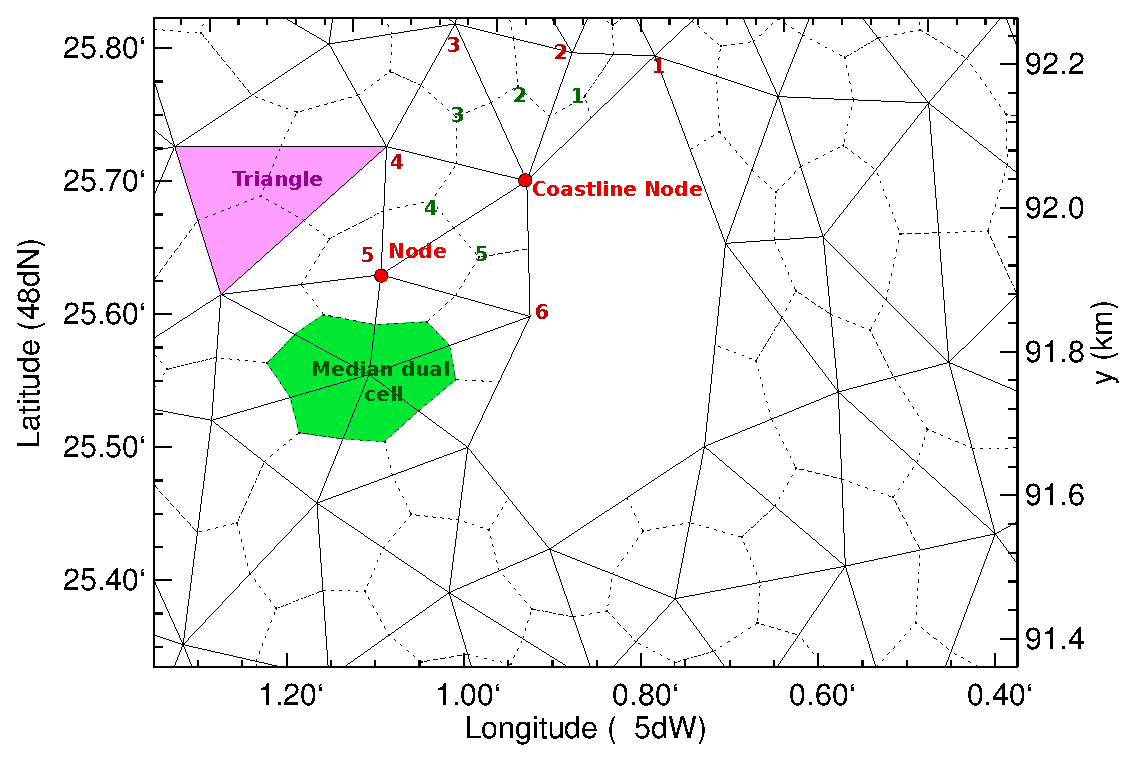
\epsfig{file=./num/grid_triangles.eps,angle=0,width=4.in}
\caption{基于三角形的网格区域示例，本例包含法国 Bannec 小岛。如果水深大于最小水深，岸线节点为活动节点。其特点是相邻节点数（所选示例中为 6）大于相邻三角形数（同一示例中为 5）。}
\label{fig:triangles} \botline
\end{center}
\end{figure}


\begin{figure} \begin{center}
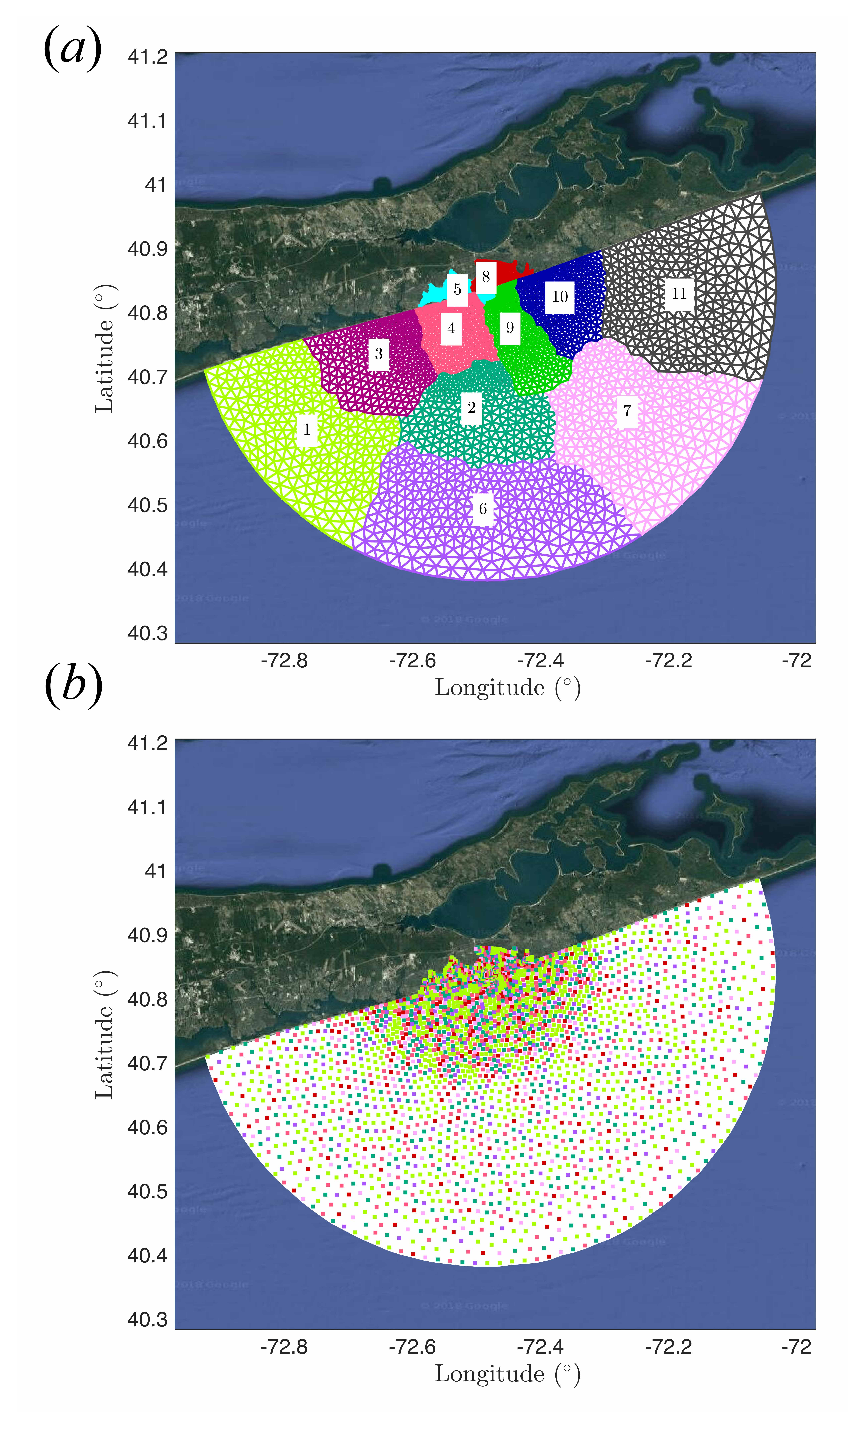
\epsfig{file=./num/DDvsCD.eps,angle=0,width=4.in}
\caption{在 11 个计算核心（以颜色表示）上，区域分解 (a) 与 Card Deck 方法 (b) 的示意差异。该网格约有 3k 个节点，针对纽约 Shinnecock Inlet 构建，取自一个 ADCIRC 示例问题。}
\label{DDvsCD} \botline
\end{center}
\end{figure}


\vssub
\subsubsection{~球面多单元（SMC）网格} \label{sub:num_space_SMC}
\opthead{SMC}{\ws (MetOffice)}{J.-G. Li}

\noindent
球面多单元（SMC）网格 \citep{art:Li11} 是 Cartesian 多单元网格 \citep{art:Li03} 向球坐标系统的扩展。它是一种非结构网格，但保留了常规经纬度网格单元，因此球坐标上的所有传播公式仍然适用，相应地所有有限差分格式也仍可使用。SMC 网格以类似于削减网格 \citep{art:RA94} 的方式放宽高纬度地区的 CFL 限制。通过转为积分方程，引入极区单元以消除微分输运方程的极点奇异性。上游非振荡二阶（UNO）平流格式 \citep{art:Li08} 已在 SMC 网格上实现，用于空间传播和谱间传播。UNO2 格式可通过 {\F PSMC} namelist 逻辑变量 {\code UNO3} 替换为三阶格式。UNO3 格式类似于 UQ 格式，但把其通量限制器替换为 UNO2 格式。波浪折射诱导旋转和大圆转向采用一种简单旋转格式 \citep{art:Li12}。对于任意时间步长，折射格式都是无条件稳定的，但最大折射诱导旋转角受到朝向局地梯度方向的最大可能折射角限制。除这一物理限制器外，{\F PSMC} namelist 中还有用户定义参数 {\code RFMAXD}，用于限制每个时间步的最大折射角。其默认值为 36.0 度。为减轻 garden sprinkler effect，使用类似 \cite{art:BH87} 的扩散项，但扩散系数简化为单一均匀参数（式~(\ref{eq:Dnn_d}) 中的 $D_{nn}$）。还可通过 {\F PSMC} namelist 逻辑变量 {\code AVERG} 使用附加的 1-2-1 加权平均格式。与常规网格相比，SMC 网格可显著减少计算时间，这得益于高纬度时间步限制的放宽以及从模式中移除陆点。为修正高纬度地区无效的标量假设，提供了一种补救方法，可将全球波浪模式扩展到整个北冰洋 \citep{art:Li16}。该 Arctic 部分可通过设置 {\F PSMC} namelist 参数 {\code Arctic=.TRUE.} 激活。

SMC 网格可用于替代规则经纬度网格，使模式区域可扩展到高纬度甚至北极，而无需缩短时间步长。除准备少量额外输入文件（包括单元数组和面数组文件）外，该应用对规则网格模式只需少量修改。单元数组可利用已有规则网格水深，仅使用海点，并在若干纬度带沿经向合并单元来生成 \citep{art:Li11}。

SMC 网格的另一个重要用途是构建多分辨率网格。基础层级 SMC 网格单元可通过把经度和纬度网格长度减半，细化为 4 个四分之一单元。该细化层级上的任意单元又可进一步划分为另外 4 个四分之一单元。这种细化可按需要继续，从而形成若干细化层级上的多分辨率网格。为保持一致，单分辨率 SMC 网格被视为只有一个层级。常规规则网格输入文件，如水深、陆海掩膜和子网格阻挡，不再需要，取而代之的是仅含海点的单元和面数组，以及一个子网格阻挡文件。水深作为整数米值存储在单元数组最后一列（第 5 列）。掩膜将在 ww3\_grid 内部用仅含海点的单元数组定义。

风和海流（若有）强迫可默认使用基础分辨率上的规则网格，作为任意 SMC 网格（单层或多层）的输入强迫。它将在模式内部插值到细化层级（若有）上。SMC 网格还可通过 {\F PSMC} namelist 中的 {\code SEAWND} 逻辑变量开启仅海点风和流输入选项。该仅海点选项不仅免除了模式内部对风（以及流，若有）插值的需要，还允许混合不同分辨率的风（以及流）强迫，并直接插值到多分辨率单元上，使其成为真正的多分辨率模式。

\begin{figure}
\centerline{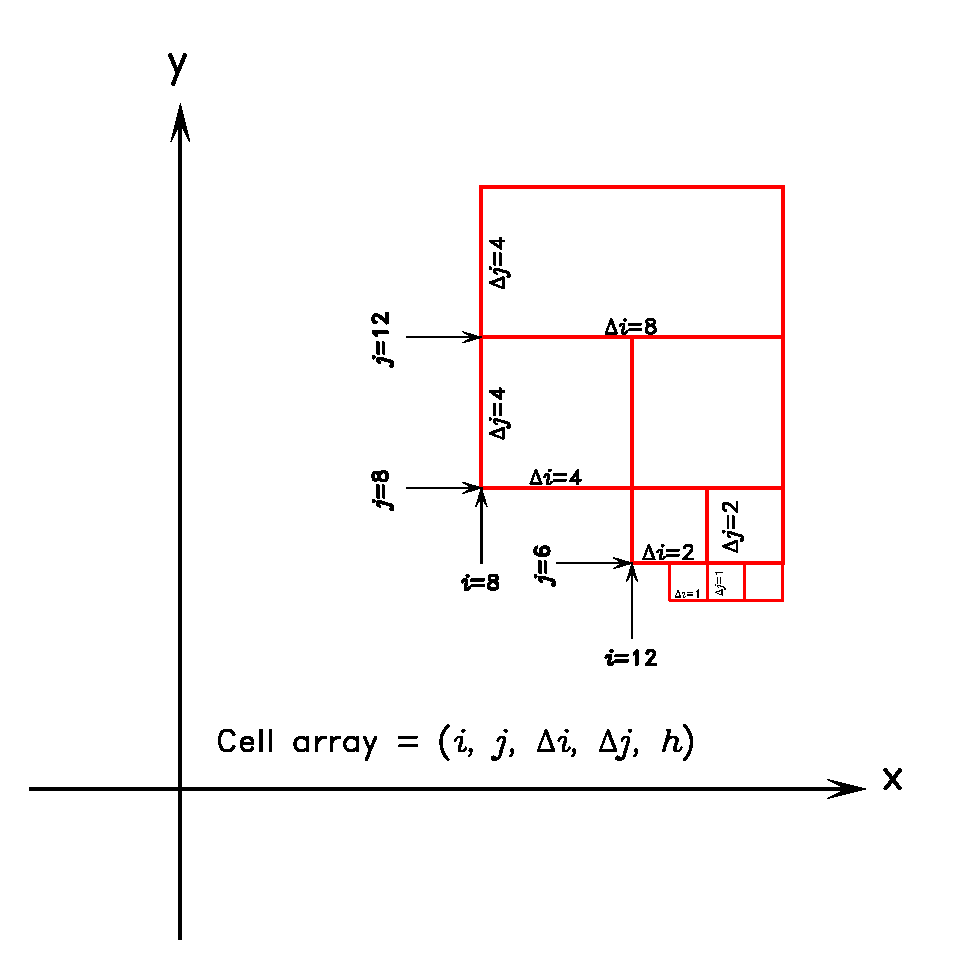
\epsfig{file=./num/smcelary.eps,angle=0,width=3.in}}
\caption{SMC 网格中使用的单元数组示意。}
\label{fig:SMCells} \botline
\end{figure}

SMC 网格的一个重要特征是它是非结构网格，也就是说，单元不要求按照其物理位置相邻排列。为便于多分辨率 SMC 网格，单元按其大小排序，使给定层级上的单元聚集在一个子循环中，共用一个子时间步。细化层级子步的基础层级时间步随网格长度一起减半。这有效避免了模式因细化单元的 CFL 限制而变慢。传播格式所需的相邻单元信息由单元面数组提供，这些面数组会针对给定单元数组列表预先计算。因此，不需要把仅含海点的 SMC 网格单元扩展到完整网格上进行传播。图~\ref{fig:SMCells} 展示了 SMC 单元数组的定义方式，图~\ref{fig:SMC_Arctic} 展示了 6-12-25 km 三层 SMC 网格中的北极区域。金色和红色圆圈分别标记 SMC6-25 网格中的全球部分和北极部分。金色圆圈内的北极部分需要固定参考方向来定义其波向箱。全球部分（直到金色圆圈）可在没有北极部分的情况下独立运行。如果用 ARC 选项激活北极部分，则从红色圆圈到金色圆圈的 4 行会在北极部分中复制为边界单元。北极部分使用单独的单元和面数组，并在波浪模式中并入全球数组用于传播。对于带输入边界条件的区域 SMC 网格，需要提供边界单元序号列表，并由 {\F PSMC} namelist 参数 {\code NBISMC} 指定边界单元数量。SMC 网格使用与规则经纬度网格相同格式的边界输入文件。边界文件可由规则网格或全球 SMC 网格模式生成，方法与规则网格一样指定边界单元中心位置。

\begin{figure}
\centerline{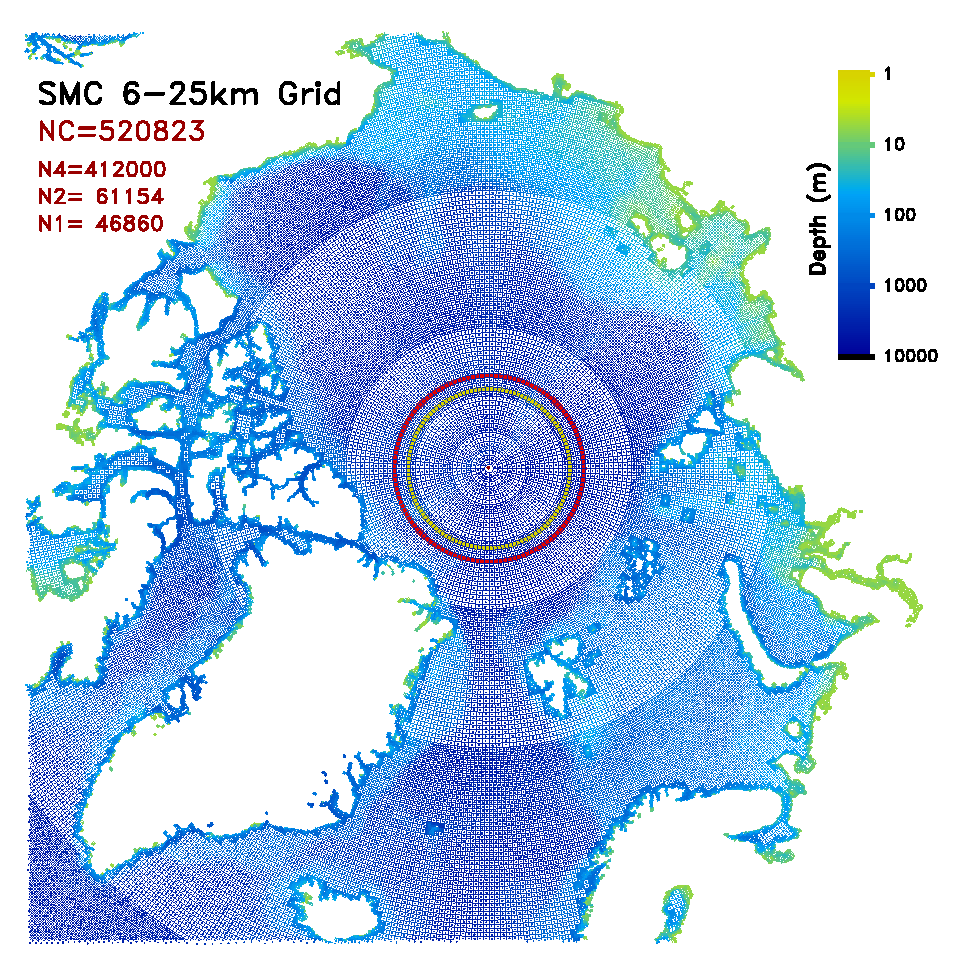
\epsfig{file=./num/JCP_Fig2_GArc.eps,angle=0,width=4.in}}
\caption{6-12-25km 多分辨率 SMC 网格中的北极区域。}
\label{fig:SMC_Arctic} 
\botline
\end{figure}

已开发若干 IDL 和 F90 程序，用于生成 SMC 网格单元和面数组，以及可视化网格网格和波场，但它们尚未正式纳入 WW3 软件包。smc\_docs/SMCG\_TKs/ 中提供了一个 IDL 程序 (Glob50SMCels.pro)，用于使用规则 50 km 网格水深文件 (G50kmBathy.dat) 生成全球 50km SMC 网格。面数组由两个 F90 程序生成，一个用于全球部分 (G50SGlSide.f90)，另一个用于北极部分 (G50SAcSide.f90)。由于极区单元的特殊处理 \citep{art:Li12}，北极极点单元的面数组需要采用不同于其他单元的方法。单元数组文件必须先用一个简单 Linux 脚本 (countcells) 排序，然后再输入面数组生成程序。面数组也需要用 Linux 脚本 (countijsd) 排序，以确定多层级子循环计数。可运行一个独立谱传播测试 (G50SMCSRGD.f90) 来测试单元和面数组，其输出可用 IDL 脚本 g50smstrspb.pro 可视化；该脚本使用 SMC 网格可视化程序 g50smcgrids.pro 保存的投影文件。通过修改 g50smcgrids.pro 中的投影参数，用户可选择投影视点（以经纬度度数表示），并保存投影供模式输出可视化使用。子网格阻挡文件可由 IDL 程序 Glob50SMCObstr.pro 生成。

SMC 网格选项的编译类似于规则经纬度网格，但需要额外开关 {\code SMC} 来调用 SMC 网格。由于 SMC 网格与规则经纬度网格共享若干网格变量，也应选择规则网格开关，例如 {\code PR2 UNO} 或 {\code PR3 UQ}。SMC 网格类型 {\code SMCTYPE} 通过在 ww3\_grid.inp 文件中用 {\code SMCG} 替换 {\code RECT} 来定义。注意，SMC 网格构建在规则经纬度网格内部，因此在 ww3\_grid.inp 文件中仍需基础分辨率层级上的规则经纬度网格参数，如 NX、NY、SX、SY、X1 和 Y1。规则经纬度网格水深、陆海掩膜和子网格阻挡输入文件不再需要，它们由 SMC 网格仅海点文件替代（水深存储在单元数组中，子网格阻挡存储在 G50GObstr.dat 中）。不过，ww3\_grid.inp 中的水深和陆海掩膜输入行会保留，用于传递最小水深等参数。由于高纬度处的合并以及可能存在的细化分辨率，规则网格映射数组会为与 SMC 网格单元保持一致而略作修改。三层 Lake Erie SMC 网格模式示例见回归测试 \emph{regtests/ww3\_tp2.10}。

SMC 网格模式的输出后处理已针对 ww3\_ounf 和 ww3\_outf 开发。对于 ww3\_ounf，用户可选择在原生模式网格海点上提取多分辨率信息，或在模式网格定义中设置的任一分辨率层级上生成规则网格。ww3\_outf 程序处理 SMC 网格数据时，可输出为基础分辨率层级上完全展开的规则经纬度网格输出，也可输出为所有 SMC 网格海点处的 ASCII 输出（type-4）。对于规则网格输出，参数值由所有与所选输出单元边界重叠的 SMC 网格单元作面积加权平均确定。海点数据的纬度和经度对应原生模式网格单元中心。对于 ww3\_ounf 海点输出，netCDF 文件中还提供描述单元大小的变量。

本代码版本未提供海点输出的可视化工具；不过，可根据请求从 Met Office 获得一些示例。针对 netCDF 海点输出，已开发一个基于 python 的 GUI 工具。所有单元 ASCII 输出可借助输入单元数组文件进行可视化，因为输出单元顺序与输入单元数组相同。IDL 脚本 g50smcswhglb.pro 是绘制全球 50km SMC 网格 SWH 输出的示例程序。它使用 g50smcgrids.pro 生成的投影文件。鼓励用户用其他语言开发自己的网格生成和后处理程序。一个 Python 小组已经成立，用于开发 SMC 网格单元和面数组生成及可视化程序。这些新的 Python 程序目前存放在一个单独的 github 站点：  
\url{https://github.com/ww3-opentools/ww3-grid/}
该站点仍处于开发阶段。欢迎 WW3 Python 程序员测试并为其改进作贡献。

从第 7 版起，SMC 网格扩展为可在 WW3 多网格模式下运行。目前，它只支持同等级 SMC 子网格并行运行。SMC 子网格的生成方式类似于具有自身边界单元列表的单个区域 SMC 网格。建议边界单元采用来自相邻子网格的复制单元，因为 SMC 子网格的边界谱交换为整谱复制粘贴，即不需要插值。规则经纬度子网格也可加入同一等级的 SMC 子网格组，但边界条件仍限于整谱交换。原始经纬度网格边界插值未启用。该简化减少了 MPI 通信负载，但如果边界单元中心未对齐，可能会损失一些精度。Great Lakes 的 SMC 子网格示例见回归测试 \emph{regtests/mww3\_test\_09}。它以 3 个 SMC 层级（0.5-1-2 km）覆盖 Lake Michigan、Huron 和 Superior，并尽量减少边界连接。
  
SMC 网格支持混合并行化；在 Cray XC40 超级计算机上使用 3 或 6 个 OpenMP 线程运行时，总耗时可减少一半。进一步增加 OpenMP 线程似乎效果不大。混合并行和多网格并行相结合，可使 \emph{mww3\_test\_09} 中 3 个 Great Lake 子网格的计算机使用规模扩展到 100 个以上节点。

建议阅读 smc\_docs/SMC\_Grid\_Guide.pdf 或会议网页上的会议论文 \citep{tol:LiS17}：
http://www.waveworkshop.org/15thWaves/
以获取更多信息；关于 SMC 网格的任何帮助，也可联系 \url{Jian-Guo.Li@metoffice.gov.uk}。


\vsssub
\subsubsection{~Garden Sprinkler Effect} \label{sub:num_GSE}
\vsssub

\noindent
高阶精度传播格式的数值扩散足够小，因此可能出现所谓的 “Garden Sprinkler Effect”（GSE）：也就是说，由于谱的离散描述，连续涌浪场会分解为一组离散涌浪场 \citep[图~3c]{art:BH87}。\ws\ 中提供了若干 GSE 缓解方法，如以下各节所述。

\addcontentsline{toc}{subsubsection}{\strut \hspace{24mm} 不进行 GSE 缓解}

\vspace{\baselineskip}
\vspace{\baselineskip}
\noindent {\bf 不进行 GSE 缓解}

\opthead{PR0 / PR1}{\ws}{H. L. Tolman}

\noindent
在无传播（开关 {\code PR0}）的情况下，或在传统网格或曲线网格中使用一阶传播格式时，既没有可用的 GSE 缓解方法，也不需要进行 GSE 缓解。

\pb
\addcontentsline{toc}{subsubsection}{\strut \hspace{24mm} Booij and Holthuijsen 1987}

\vspace{\baselineskip} 
\vspace{\baselineskip} 
\noindent {\bf Booij and Holthuijsen 1987}

\opthead{PR2}{\ws}{H. L. Tolman}


经典 GSE 缓解方法来自 \cite{art:BH87}。他们为离散谱推导了另一种传播方程，其中包含扩散修正，以便在谱描述离散的情况下仍能考虑连续色散。该修正只影响空间传播；对于一般空间坐标 $(x,y)$，其形式为

% ------ Correction linear dispersion --------- %
% eq:d_bal_0         Booij and Holthuijsen, 1987
% eq:Dxx
% eq:Dyy
% eq:Dxy
% eq:Dss
% eq:Dnn

\begin{equation}
\frac{\p \cN}{\p t} +
\frac{\p}{\p x} \left [ \dot{x} \cN 
           - D_{xx} \frac{\p \cN}{\p x} \right ] +
\frac{\p}{\p y} \left [ \dot{y} \cN 
           - D_{yy} \frac{\p \cN}{\p y} \right ] -
2 D_{xy} \frac{\p^2 \cN}{\p x \p y} = 0
\: , \label{eq:d_bal_0}\end{equation}  \begin{equation}
D_{xx} = D_{ss} \, \cos^2 \theta + D_{nn} \, \sin^2 \theta
\: , \label{eq:Dxx} \end{equation} \begin{equation}
D_{yy} = D_{ss} \, \sin^2 \theta + D_{nn} \, \cos^2 \theta
\: , \label{eq:Dyy} \end{equation}  \begin{equation}
D_{xy} = ( D_{ss} - D_{nn} ) \, \cos \theta \, \sin \theta
\: , \label{eq:Dxy} \end{equation} \begin{equation}
D_{ss} = (\Delta c_g )^2 \: T_s / 12
\: , \label{eq:Dss} \end{equation} \begin{equation}
D_{nn} =  ( c_g \Delta \theta )^2 \: T_s / 12
\: , \label{eq:Dnn} \end{equation}

\noindent
其中 $D_{ss}$ 是离散波分量传播方向上的扩散系数，$D_{nn}$ 是沿该离散波分量波峰方向的扩散系数，$T_s$ 是自涌浪生成以来经过的时间。在当前分步法中，扩散可作为单独步骤加入：

% eq:d_bal_1         Separated diffusion equation

\begin{equation}
\frac{\p \cN}{\p t} = 
\frac{\p}{\p x} \left [ D_{xx} \frac{\p \cN}{\p x} \right ] +
\frac{\p}{\p y} \left [ D_{yy} \frac{\p \cN}{\p y} \right ] +
   2 D_{xy} \frac{\p^2 \cN}{\p x \p y}
\: . \label{eq:d_bal_1} \end{equation}

\noindent
该方程在实现时采用两个简化，其合理性见 \cite{tol:OMB95} 的讨论。第一，涌浪“年龄” $T_s$ 在整个模式中保持常数（由用户定义，没有默认值）。第二，扩散系数 $D_{ss}$ 和 $D_{nn}$ 按深水假设计算：

% eq:Dss_d
% eq:Dnn_d

\begin{equation}
D_{ss} = \left ( \: (X_\sigma-1) \: \frac{\sigma_m}{2 k_m} \right )^2
\: \frac{T_s}{12} \: , \label{eq:Dss_d} \end{equation} \begin{equation}
D_{nn} =  \left ( \frac{\sigma_m}{2 k_m} \Delta \theta \right )^2
\: \frac{T_s}{12} \: , \label{eq:Dnn_d} \end{equation}

\noindent
其中 $X_\sigma$ 按式~(\ref{eq:sigma_grid}) 定义。采用这两个假设后，对于每个独立谱分量，扩散张量在整个空间区域内为常数。

式~(\ref{eq:d_bal_1}) 用前向时间、中心空间格式求解。在 $\phi$ ($x$) 空间中点 $i$ 与 $i-1$ 之间的单元界面处，式~(\ref{eq:d_bal_1}) 右端第一项中方括号内的项（记为 $\cD_{i,-}$）估计为

% eq:ddif_1          Discrete diffusion 1

\begin{equation}
D_{xx} \frac{\p \cN}{\p x} \approx \cD_{i,-} =
\left . D_{xx} \; \left ( \frac{\cN_i - \cN_{i-1}}{\Delta x} \right ) \: 
\right |_{j,l,m} \: . \label{eq:ddif_1} \end{equation}

\noindent
计数器为 $i$ 和 $i+1$ 的相应值，以及 $\lambda$ ($y$) 空间中的梯度，仍通过轮换索引和增量得到。如果两个网格点之一位于陆地上，则式~(\ref{eq:ddif_1}) 设为零。式~(\ref{eq:d_bal_1}) 右端的混合导数（记为 $\cD_{ij,--}$）在 $x$ 空间中的网格点 $i$ 和 $i-1$、以及 $y$ 空间中的 $j$ 和 $j-1$ 上估计为

% eq:ddif_2          Discrete diffusion 2

\begin{equation}
\cD_{ij,--} = \left . \: D_{xy} 
\left ( \frac{- \cN_{i,j} + \cN_{i-1,j} +
              \cN_{i,j-1} - \cN_{i-1,j-1}}
           {0.5 ( \Delta x_j + \Delta x_{j-1} ) \: \Delta y}
              \right ) \: \right |_{l,m} 
\: . \label{eq:ddif_2} \end{equation}

\noindent
注意，由于使用球面网格，增量 $\Delta x$ 是 $y$ 的函数。只有当所考虑的四个网格点全为海点时才计算该项，否则将其设为零。对式~(\ref{eq:d_bal_1}) 中第一项采用时间前向离散，对右端第一项和第二项的其余部分采用空间中心离散，最终算法为

% eq:ddif_3          Discrete diffusion 3

\begin{eqnarray}
\cN_{i,j,l,m}^{n+1} = \cN_{i,j,l,m}^n + 
\frac{\Delta t}{\Delta x} 
   \left ( \cD_{i,+} - \cD_{i,-} \right ) +
\frac{\Delta t}{\Delta y}
   \left ( \cD_{j,+} - \cD_{j,-} \right ) \nonumber \\
+ \frac{\Delta t}{4} \left ( \cD_{ij,--} + 
   \cD_{ij,-+} + \cD_{ij,+-} + \cD_{ij,++} \right )
\: . \label{eq:ddif_3} \end{eqnarray}

\noindent
当满足下式时可得到稳定解 \citep[e.g.,][Part I section 7.1.1]{bk:Fle88}：

% eq:ddif_4          Stability

\begin{equation}
\frac{D_{\max} \: \Delta t}{\min(\Delta x , \Delta y)^2}
\leq 0.5 \: , \label{eq:ddif_4} \end{equation}

\noindent
其中 $D_{\max}$ 为扩散系数的最大值（通常 $D_{\max} = D_{nn}$）。由于该稳定性判据是网格增量的二次函数，在大尺度应用的高纬度地区，稳定性可能成为严重问题。为避免这对模式时间步长造成过度约束，使用修正涌浪年龄 $T_{s,c}$：

% eq:Ts_cor

\begin{equation}
T_{s,c} = T_s \min \left \{ \: 1 \: , \: 
\left ( \frac{\cos(\phi)}{\cos(\phi_c)} \right )^2 \: \right \}
\: , \label{eq:Ts_cor} \end{equation}

\noindent
其中 $\phi_c$ 是用户定义的截止纬度。

\vspace{\baselineskip} \noindent
 
上述扩散是涌浪传播所需要的，但对增长中的风海并不真实。对于风海，不带色散修正的 \uq{} 格式已经足够平滑，可以给出稳定的有限风区增长曲线 \citep{tol:OMB95}。为去除轻微振荡，对增长中的波分量使用小的各向同性扩散。为保证该扩散较小且对所有谱分量等效，它由预设的单元 Reynolds（或单元 Peclet）数 $\cR = c_g \Delta x D_g^{-1} = 10$ 计算，其中 $D_g$ 是增长分量的各向同性扩散：

% eq:Dg              Diffusion growing components

\begin{equation}
D_g = \frac{c_g \: \min(\Delta x , \Delta y)}{\cR} \: . \label{eq:Dg}
 \end{equation}

\noindent
涌浪和风海的扩散按无量纲风速或反波龄 $u_{10} c^{-1} = u_{10} k \sigma^{-1}$ 进行线性组合：

% eq:Xg              Linear combination for diffusion
% eq:Dss_f           Final Dss
% eq:Dnn_f           Final Dnn

\begin{equation}
X_g = \min \: \left \{ \: 1 \: , \: \max \: \left [ \: 0 \: , \:
3.3 \left ( \frac{k \, u_{10}}{\sigma} \right ) - 2.3
\: \right ] \: \right \}
 \: , \label{eq:Xg} \end{equation} \begin{equation}
D_{ss} = X_g D_g + (1-X_g) D_{ss,p}
\: , \label{eq:Dss_f} \end{equation} \begin{equation}
D_{nn} = X_g D_g + (1-X_g) D_{nn,p}
\: , \label{eq:Dnn_f} \end{equation}

\noindent
其中后缀 $p$ 表示式~(\ref{eq:Dss_d}) 和 (\ref{eq:Dnn_d}) 中定义的传播扩散。式~(\ref{eq:Dg}) 和 (\ref{eq:Xg}) 中的常数在模式中预设。


\pb
\addcontentsline{toc}{subsubsection}{\strut \hspace{24mm} 空间平均}

\vspace{\baselineskip} 
\vspace{\baselineskip} 
\noindent {\bf 空间平均}

\opthead{PR3}{\ws}{H. L. Tolman}


上述 GSE 缓解方法的主要缺点，是它可能影响模式经济性；这与式~(\ref{eq:ddif_4}) 有关，并在 \cite{tol:Waves01a,tol:OMOD02b} 中有讨论。因此，\ws\ 又开发了一种替代的附加 GSE 缓解方法。

该方法是 \ws\ 的默认方法，它用一个单独的分步替代附加扩散步骤 (\ref{eq:d_bal_1})；在该分步中，对给定谱分量的能量密度场进行直接平均。每个网格点周围用于平均的区域，在传播方向 ($\bs$) 和法向方向 ($\bn$) 上分别延伸为

\begin{equation}
\pm \gamma_{a,s} \: \Delta c_g \: \Delta t \: \bs \:\:\: ,
\pm \gamma_{a,n} \: c_g \Delta \theta \: \Delta t \: \bn \:\:\: , \label{eq:GSE_avg}
\end{equation}

\noindent
其中 $\gamma_{a,s}$ 和 $\gamma_{a,n}$ 为可调常数，默认值设为 1.5。该平均过程如图~\ref{fig:GSE_1} 所示。注意，如 \cite{tol:OMOD02b} 所讨论，在实际应用中这些值可能需要重新调整。该文附录 A 给出了平均格式的细节，包括守恒性方面的考虑。此外，与 \cite{art:BH87} 方法保持一致意味着 $\gamma_{a,s}$ 和 $\gamma_{a,n}$ 应随空间网格分辨率变化 \citep[见][Appendix]{tol:OMOD08a}。

注意，具有主导方向 $\bs$ 和 $\bn$ 的这种平均类似于 \cite{art:BH87} 的扩散方法，后者使用相同主方向。然而，该平均方法绝不会影响时间步长，因为它与实际传播完全分离。此外，如果使用显式格式，通常有 $c_g \Delta t / \Delta x < 1$，那么显然按 (\ref{eq:GSE_avg}) 定义的区域进行平均，一般只需要直接相邻空间网格点的信息，如图~\ref{fig:GSE_1} 所示。此外，该方法不需要高纬度滤波。

\begin{figure} \begin{center}
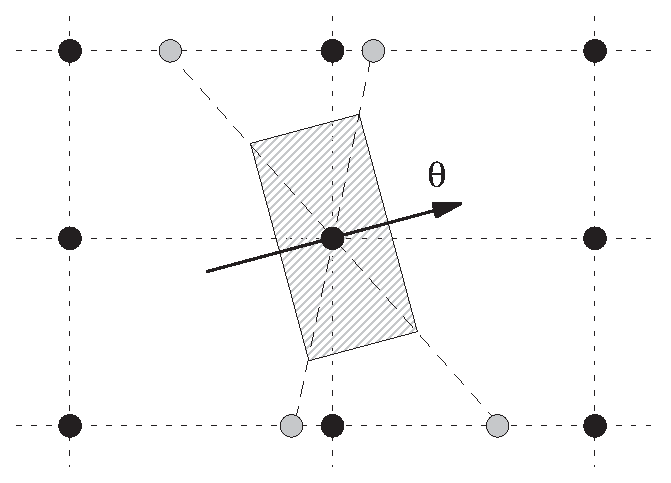
\epsfig{file=./num/GSE_1.eps,angle=0,width=2.2in}
\caption{空间平均 GSE 缓解技术示意图。实心圆和虚线表示空间网格。阴影区域表示需要考虑的平均区域。角点值由中心网格点和灰色点得到；后者通过相邻网格点插值得到 \citep[引自][]{tol:OMOD02b}。}
\label{fig:GSE_1} \botline
\end{center}
\end{figure}

如 \cite{tol:OMOD02b,tol:OMB02b} 所示，该方法给出的结果几乎与前一种方法相同，但计算成本略低。对于高分辨率应用，平均方法可能显著更经济。



最后，通过保证离散谱方向不与空间网格线重合，也可在一定程度上缓解 GSE。这可通过把第一个离散方向 $\theta_1$ 定义为

% eq:theta1          First direction

\begin{equation}
\theta_1 = \alpha_\theta \: \Delta \theta \:\:\: , \label{eq:theta1}
\end{equation}

\noindent
其中 $-0.5 \leq \alpha_\theta \leq 0.5$ 可由用户定义。注意，设置 $\alpha \neq 0$ 有利于一阶格式，但对三阶格式影响可忽略。
 

\pb
\vsssub
\subsubsection{~未解析障碍物} \label{sub:num_obst}
\conthead{\ws}{H. L. Tolman, L. Mentaschi}

\noindent
即使在 \ws\ 1.15 版最初调参时 \citep{tol:OMB02a}，也已清楚未解析岛群是局地波浪模式误差的主要来源。这一点在 \citet[][图~3]{tol:Waves01a} 和 \citet[][图~8]{tol:WaF02} 中有更详细说明。在 \ws\ 中，有两种方法可用于参数化未解析障碍物。第一种方法最初来自 \swan\ \citep{art:BRH99,man:SWAN3}，它在数值格式内部的空间网格单元边界处施加未解析障碍物的影响，并已用于规则网格。第二种方法由 \citep{art:Mentaschi2015b} 提出，基于源项，可应用于不同网格类型。本节介绍第一种方法；第二种方法的说明见第 \ref{sec:UOST} 节。

在基于传播的方法中，通过单元公共边界的数值通量会按照未解析障碍物提供的阻挡程度受到抑制。在该方法中，式~(\ref{eq:uq_xy_tot}) 的 \uq{} 格式数值传播格式修改为

% eq:uq_xy_obstr

\begin{equation}
\cN_{i,j,l,m}^{n+1} = \cN_{i,j,l,m}^n +
\frac{\Delta t}{\Delta \phi} \left [ \alpha_{i,-} \cF_{i,-} - \alpha_{i,+} \cF_{i,+} \right ]
\: , \label{eq:uq_xy_obstr} \end{equation}

\begin{figure} \begin{center}
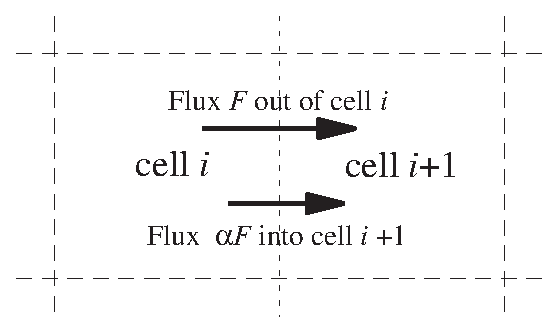
\epsfig{file=./num/obstr.eps,angle=0,width=2.2in}
\caption{未解析障碍物的处理。公共单元边界（点线）的透明度为 $\alpha$。虚线表示其他单元边界。数值通量从左向右。}
         \label{fig:obstr} \botline
\end{center}
\end{figure}

\noindent
其中 $\alpha_{i,-}$ 和 $\alpha_{i,+}$ 是相应单元边界的“透射率”，范围从 0（封闭边界）到 1（无遮挡）。对于出流边界，透明度按定义为 1，否则能量会在单元中人为累积。对于入流边界，小于 1 的透明度会导致受阻能量在单元边界处被移除。该方法如图~\ref{fig:obstr} 所示。注意，类似方法很容易应用于一阶和二阶格式。还需注意，\cite{art:HY96} 和 \cite{art:HMM00} 曾使用另一种障碍物方法，其中障碍物是谱方向 $\theta$ 的函数。

模式中有两种定义障碍物的方法。第一种方法直接在网格边界处定义障碍物。这需要生成交错的水深-透明度网格。第二种方法允许用户在同一网格上定义水深和透明度。在这种情况下，入流边界处的透明度为 $0.5(1+\alpha_i)$，而出流透明度按定义为 1。为完成总透明度 $\alpha_i$，流向上的下一个单元将具有入流透明度 $2\alpha_i/(1+\alpha_i)$。如果连续单元均部分受阻，则采用各个透明度的乘积。

该方法也可用于连续模拟冰覆盖对波浪传播的影响。这一点在 \para\ref{sub:num_ice} 中讨论。岛屿和海冰的子网格处理细节见 \cite{tol:OMOD03a}。该方法在大尺度波浪模式中的影响研究见 \cite{tol:OMB02b,tol:OMOD03a}。

\ws\ 的默认设置是不包括障碍物的子网格建模。生成阻挡网格可能非常耗费人力。因此，\cite{tol:MMAB07a, tol:OMOD08a} 开发了一种自动生成海底和阻挡网格的方法。注意，该选项不涉及编译级选择，而完全由网格预处理器控制（见第 \ref{chapt:run} 章）。


\vsssub
\subsubsection{~连续移动网格} \label{sub:num_move}
\opthead{MGx}{\ws}{H. L. Tolman}

\addcontentsline{toc}{subsubsection}{\strut \hspace{24mm} 一般概念}


为处理飓风等快速变化、小尺度条件下的波浪增长问题，模式 3.02 版加入了一个选项，可向网格添加给定的连续平流速度。该模式版本在 \cite{tol:OMOD05b} 中有详细说明。这里仅给出简要描述。



\begin{center}
\rule[1mm]{55mm}{1.0mm} WARNING \rule[1mm]{55mm}{1.0mm} \\
 \vspace{\baselineskip}
\parbox{120mm}{\ws\ 的连续移动网格版本仅用于在高度理想化条件下测试波浪模式性质。该模式版本只应在无平均流、无陆块的深水条件下使用。此外，为避免大圆传播带来的复杂性，只应使用 Cartesian 网格。该选项也仅针对传播选项 {\F pr1} 和 {\F pr3} 实现。注意，无论在编译阶段还是运行阶段，脚本或程序都不会检查这些条件。该选项不被视为适合一般应用。} \\
\vspace{\baselineskip}
\rule[1mm]{55mm}{1.0mm} WARNING \rule[1mm]{55mm}{1.0mm}
\end{center}

\noindent
对于上述应用，式~(\ref{eq:bal_plane}) 可写为

\begin{equation}
\frac{\partial N}{\partial t} + 
\left ( {\bf\dot{x}}-{\bf{v}}_g \right ) \cdot \nabla_x N  = 
\frac{S}{\sigma} \: , \label{eq:bal_move}
\end{equation}

\noindent
其中 ${\bf{v}}_g$ 表示网格的平流速度。该选项在编译模式时选择。第二个编译级选项允许把网格平流速度 ${\bf{v}}_g$ 加到风场上。这样提供了一种简单方法，可保证风场质量守恒不依赖于实际和瞬时的网格平流速度。平流速度 ${\bf{v}}_g$ 可随时间变化，并由用户在模式运行时提供（见下文）。




在式~(\ref{eq:bal_move}) 适用的简化条件下，如果考虑到该方程等价于

\begin{equation}
\frac{\partial N}{\partial t} + 
\nabla_x \cdot \left ( {\bf\dot{x}}-{\bf{v}}_g \right ) N  = 
\frac{S}{\sigma} \: , \label{eq:bal_move2}
\end{equation}

\noindent
则移动网格的实现很直接。这又意味着，对于求解式~(\ref{eq:bal_plane}) 的任意数值格式，平流速度 ${\bf{v}}_g$ 可直接加到 ${\bf\dot{x}}$ 中。由于这会影响净平流速度，也会影响稳定性特征。该影响已通过在式~(\ref{eq:dtpl}) 的实际传播时间步长计算中包含移动网格速度而自动考虑。因此，用户只需提供代表 $\bf{v}_g = 0$ 情形的合适最大传播时间步长。

由于频率相同但传播方向不同的谱分量在网格中的停留时间不同，网格运动会对 Garden Sprinkler Effect (GSE) 产生表观影响。当前 GSE 缓解方法对较年轻涌浪往往比对较老涌浪更有效。因此，在移动网格中停留时间较长的涌浪往往表现出更明显的 GSE \citep[见][]{tol:OMOD05b}。为缓解 GSE 缓解中的这种表观不平衡，将式~(\ref{eq:GSE_avg}) 替换为

\begin{equation}
\pm \gamma_a \gamma_{a,s} \: \Delta c_g \: \Delta t \: \bs \:\:\: ,
\pm \gamma_a \gamma_{a,n} \: c_g \Delta \theta \: \Delta t \: \bn \:\:\: ,
\label{eq:move_GSE_avg1}
\end{equation}

\begin{equation}
\gamma_a = \left ( \frac{|\dot{\bf{x}}|}{|\dot{\bf{x}}-\bf{v}_g|}
\right ) ^{p}
\label{eq:move_GSE_avg2}
\end{equation}

\noindent
其中 $\gamma_a$ 是考虑网格运动的修正因子，幂次 $p$ 是允许一定调节的参数。采用该修改后，可根据相应谱分量在移动网格中的预期停留时间，重新缩放所施加的平滑量，从而使 GSE 影响在网格上分布得更均匀 \citep[见][]{tol:OMOD05b}。


为开启移动网格选项或风场/GSE 修正，在 \ws\ 源代码中加入了三个可选开关（另见 \para\ref{sec:switches}）：

\begin{slist}
\sit{mgp} {Apply advection correction for continuous moving grid.}
\sit{mgw} {Apply wind correction for continuous moving grid.}
\sit{mgg} {Apply GSE alleviation for
           continuous moving grid.}
\end{slist}

\noindent
平流速度和方向输入到 shell 的方式类似于均匀流输入（见第~\ref{sec:ww3shel} 节中 {\file ww3\_shel.inp} 文件底部），只是把关键字 `{\code CUR}' 换为 `{\code MOV}'。与所有均匀输入场一样，平流速度可随时间变化。移动网格模式运行示例见测试算例 {\file ww3\_ts3}。第 \ref{sec:ww3multi} 节中的 {\file ww3\_multi.inp} 也有类似能力，并在测试算例 {\file mww3\_test\_05} 中测试。

\vssub
\subsubsection{~旋转网格} \label{sub:num_space_rotagrid}
\opthead{RTD}{\ws\ (MetOffice)}{J.-G. Li}

\noindent
旋转网格是一种纬度-经度（lat-lon）网格，通过沿经度 $\lambda_{p}$ 旋转北极，使其在标准纬度-经度系统中移到纬度 $\phi_{p}$ 的新位置得到。选择新的极点位置，是为了可将目标模式区域放在旋转赤道区域附近，从而得到间距更均匀的经纬度网格。因此，旋转网格也称为\emph{赤道网格}。例如，UK Met Office 使用的 North Atlantic and European wave (NAEW) 模式采用位于 37.5N、177.5E 的旋转极点，使英国伦敦（\textasciitilde{}51.5N 0.0E）几乎位于旋转赤道上。与同一区域中的标准经纬度网格相比，该旋转网格可在 NAEW 区域内提供间距均匀得多的经纬度网格。

在 \ws\ 中，旋转网格以对原始经纬度网格最小修改的方式实现。实际上，在模式内部旋转网格的处理就像标准经纬度网格一样。若要建立并运行旋转网格模式配置，用户应选择规则经纬度网格并使用 {\code RTD} 开关。旋转极点位置通过输入文件 {\bf ww3\_grid.inp} 中 {\code ROTD} namelist 下的 {\code PLAT} 和 {\code PLON} 变量设置（见第~\ref{sec:config011} 节）。如果极点设置为 {\code PLAT = 90.0}、{\code PLON = -180.0}，则该网格按标准经纬度系统处理。

风、流和冰文件等模式输入文件应映射到旋转网格上。为方便在标准经纬度网格框架中嵌套，提供给旋转网格以及从旋转网格输出的边界条件数据，使用以标准网格北向为参考的谱和标准经纬度网格点值；这些值会在 \ws\ 内部转换为旋转网格经纬度。{\bf ww3\_shel.inp} 或 {\bf ww3\_shel.nml} 中的二维谱输出位置列表也用标准经纬度指定。

当从标准网格嵌套到旋转网格模式时，外层和内层网格对应的模式可执行文件都应在编译时设置 {\code RTD} 开关。当从旋转网格嵌套到标准网格模式时，内层（标准）网格模式不需要用 {\code RTD} 编译。

输出到单向嵌套内层网格边界点的谱按附录~\ref{app:nest} 所述传递。输出边界条件在输入文件中定义（见 {\bf ww3\_grid.inp}，第~\ref{sec:config011} 节），形式为以内层网格坐标给出的一系列直线。如果内层网格为旋转网格，则其极点位置必须在外层网格的 {\code ROTB} namelist 下定义为数组元素 {\code BPLAT(\sl{n})} 和 {\code BPLON(\sl{n})} 的值。数组索引 {\sl{n}} 是边界条件文件 {\file nest{\sl{n}}.ww3} 的索引（{\sl{1:9}}）。

旋转网格的模式方向输出和 x-y 矢量输出可通过把 {\bf ww3\_grid.inp} 的 ROTD namelist 中 UNROT 变量设为 True，转换为标准网格北向参考。采用该设置后，对于点输出经纬度位置，所有方向值如风向、流向和二维谱都会转换为标准经纬度取向。用于反旋转网格化场的函数应用在 {\bf ww3\_ounf}、{\bf ww3\_outf} 和 {\bf ww3\_grib} 中。运行 {\bf ww3\_ounf} 和 {\bf ww3\_ounp} 时，生成的 netCDF 文件将包含变量属性 direction\_reference，用于说明使用的是标准（真北）方向参考系还是旋转网格方向参考系。由 {\bf ww3\_ounf} 生成的网格化 netCDF 文件还包含 \emph{standard\_latitude} 和 \emph{standard\_longitude} 二维数组，用于描述旋转模式单元中心在标准经纬度参考系中的位置。

如果用户希望使用 {\bf ww3\_bound} 或 {\bf ww3\_bounc} 边界处理程序为旋转极点网格生成边界条件，需要注意这些程序的输入谱始终预期在\emph{标准极点}上表述。

模块 {\bf w3servmd.ftn} 中提供了六个用于旋转网格转换的子程序：
\begin{vlist}
\vit{w3spectn}{}{Turns wave spectrum anti-clockwise by AnglD}
\vit{w3acturn}{}{Turns wave action(k,nth) anti-clockwise by AnglD}
\vit{w3thrtn}{}{Turns direction parameters anti-clockwise by AnglD}
\vit{w3xyrtn}{}{Turns x-y vector parameters anti-clockwise by AnglD}
\vit{w3lltoeq}{}{Convert standard into rotated lat/lon plus AnglD}
\vit{w3eqtoll}{}{Reverse of w3lltoeq, but AnglD unchanged}
\end{vlist}
这些子程序是自包含的，可从模式中提取出来，用于旋转网格文件的前处理或后处理。已有一些基于这些子程序开发的转换工具，但尚未包含在 \ws\ 中。旋转网格模式（NAEW）的示例见回归测试 \emph{regtests/ww3\_tp2.11}。用户可在 \emph{smc\_docs/Rotated\_Grid.pdf} 中找到更多信息，或联系 Jian-Guo Li 获取帮助（\url{Jian-Guo.Li@metoffice.gov.uk}）。

\vssub
\subsection{~谱内传播} \label{sub:spec}
\vssub
\subsubsection{~一般概念}
\vsssub

数值分步算法的第三步考虑折射和残余（流致）波数偏移。无论空间网格离散和坐标系统如何，该步骤中要求解的方程为

%-----------------------------------%
% Step : Intra-spectral propagation %
%-----------------------------------%
% eq:step_intra
% eq:k_dot_g

\begin{equation}
\frac{\p N}{\p t} + \frac{\p}{\p k} \, \dot{k}_g N +
\frac{\p}{\p \theta} \, \dot{\theta}_g N = 0
\: , \label{eq:step_intra} \end{equation} \begin{equation}
\dot{k}_g  = \frac{\p \sigma}{\p d} 
    \frac{{\bf U} \cdot \nabla_x d}{c_g}  -
    {\bf k} \cdot \frac{\p {\bf U}}{\p s}
\: , \label{eq:k_dot_g} \end{equation}

\noindent
其中 $\dot{k}_g$ 是相对于网格的波数速度，$\dot{\theta}_g$ 由 (\ref{eq:theta_g_dot}) 和 (\ref{eq:theta_dot}) 给出。该方程在 $\theta$ 空间中不需要边界条件，因为模式按定义使用完整（闭合）的方向空间。然而，在 $k$ 空间中需要边界条件。在低波数处，假定离散区域之外不存在波作用量。因此，假定在离散低波数边界处没有作用量进入模式。在高波数边界处，跨离散边界的输运按式~(\ref{eq:tail_N_k}) 给出的参数化谱形计算。计算 $\dot{\theta}$ 时所需的水深导数主要使用中心差分确定。不过，对于靠近陆地的点，只使用海点的一侧差分。

$\theta$ 空间中的传播可能在显式数值格式中造成实际问题，因为对于极浅水中的长波，或由于强流切变，折射速度可能变得极大。类似地，$k$ 空间中的传播在极浅水中也会遇到类似问题。为避免因折射而需要极小时间步长，对 $\theta$ 空间和 $k$ 空间中的传播速度 (\ref{eq:theta_dot}) 进行滤波：

% eq:theta_filter

\begin{equation}
\dot{\theta} = X_{rd}(\lambda,\phi,k)\left( \dot{\theta_d} + 
\dot{\theta_c} + \dot{\theta_g} \right)\: , \label{eq:theta_filter} \end{equation}

\noindent
其中下标 $d$、$c$ 和 $g$ 分别指 (\ref{eq:theta_dot}) 中折射速度与水深、流和大圆相关的部分。滤波因子 $X_{rd}$ 对每个波数和位置分别计算，并被确定为使由\emph{水深}折射项导致的 $\theta$ 空间传播 \cfl{} 数不超过预设（用户定义）值（默认 0.7）。这对应于对某些低频波分量减小海底坡度。对于中纬度，受影响分量预期携带很少能量，因为它们位于极浅水中。携带显著能量的长波分量通常正向海岸传播，其能量无论如何都会被耗散。该滤波对短波以及靠近极点处也很重要。可通过减小谱内折射时间步长，并查看模式输出中的最大 CFL 数来测试该滤波的影响。这些最大 CFL 数在滤波应用之前计算。

% \vspace{\baselineskip}
% \centerline{\ldots ADD DYNAMIC TIME INTEGRATION \ldots}


为适应非线性相互作用 $S_{nl}$ 的计算，谱空间始终采用常数方向增量和对数频率网格 (\ref{eq:sigma_grid}) 离散。可使用一阶、二阶和三阶格式，并在以下各节介绍。

\vssub
\subsubsection{~一阶格式}
\opthead{PR1}{\ws}{H. L. Tolman}

\noindent
在一阶格式中，$\theta$ 和 $k$ 空间中的通量使用式~(\ref{eq:1up_xy_1}) 至 (\ref{eq:1up_xy_3}) 计算（将 $\cN$ 替换为 $N$，并轮换相应计数器）。完整的一阶格式为

% eq:1up_intra_tot

\begin{equation}
N_{i,j,l,m}^{n+1} = N_{i,j,l,m}^n 
 + \frac{\Delta t}{\Delta \theta} \left [ \cF_{l,-} - \cF_{l,+} \right ]
 + \frac{\Delta t}{\Delta k_m} \left [ \cF_{m,-} - \cF_{m,+} \right ]
\: , \label{eq:1up_intra_tot} \end{equation}

\noindent
其中 $\Delta \phi$ 为方向增量，$\Delta k_m$ 为（局地）波数增量。低波数边界条件通过对 $m=1$ 取 $\cF_{m,-}=0$ 施加；高波数边界条件则使用参数化近似 (\ref{eq:tail_N_k}) 计算 $N$，即把离散网格向高波数方向扩展一个网格点。

\vssub
\subsubsection{~二阶格式 (UNO)}
\opthead{UNO}{Met Office}{J.-G. Li}

\noindent
对于方向 $\theta$ 空间，UNO 格式与规则网格上的格式相同，前提是假定方向箱间距规则。然而，对于 \emph{k} 空间，UNO 格式使用其不规则版本；该版本用局地梯度而不是差分，估计谱箱 \emph{i}-1 与 \emph{i} 之间单元面中通量点处的波作用量值，即
\begin{equation}
  N_{i-}^{*}=N_{c}+sign\left(N_{d}-N_{c}\right)\frac{\left(\Delta
      k_{c}-|\dot{k}_{i-}|\Delta
      t\right)}{2}\min\left(|\frac{N_{u}-N_{c}}{k_{u}-k_{c}}|,|\frac{N_{c}-N_{d}}{k_{c}-k_{d}}|\right)
  \:\:\:,
\label{eq:UNO2irregular}
\end{equation}

\noindent
其中 \emph{i}- 为波数 \emph{k} 箱索引；下标 \emph{u}、\emph{c} 和 \emph{d} 分别表示相对于给定 \emph{i}- 面速度 $\dot{k}_{i-}$ 的\emph{上游、中心}和\emph{下游}单元；$k_{c}$ 为中心箱波数，$\Delta k_{c}$ 为中心箱宽度。不规则网格 UNO 格式的细节见 \cite{art:Li08}。

$\theta$ 空间的边界条件是自然周期条件。对于 \emph{k} 空间，由于 UNO 格式为二阶精度，在波谱区域两端各增加两个零谱箱。



\vssub
\subsubsection{~三阶格式 (UQ)}
\opthead{UQ}{\ws}{H. L. Tolman}

\noindent
$\theta$ 空间中的 \uq{} 格式采用与物理空间格式类似的方式实现，区别在于封闭的方向空间不需要边界条件。$k$ 空间中的可变网格间距需要对格式作若干修改，如 \cite[{Appendix}]{art:Leo79} 所述。于是式~(\ref{eq:quick_1}) 至
(\ref{eq:quick_4}) 变为

% ------ QUICKEST scheme for k space---------- %
% eq:quick_1k        Basic flux
% eq:quick_2k        Boundary value
% eq:quick_3k        Divergence
% eq:quick_4k        CFL number

\begin{equation}
\cF_{m,-} = \left [ \dot{k}_{g,b} \: N_b \: \right ]^n_{i,j,l}
\: , \label{eq:quick_1k}\end{equation} \begin{equation}
\dot{k}_{g,b} = 0.5 \: \left ( \dot{k}_{g,m-1} + \dot{k}_{g,m} 
\: \right )  \: , \label{eq:quick_1ak}
\end{equation} \begin{equation}
N_b = \frac{1}{2} \left [ \rule[0mm]{0mm}{\baselineskip} \: 
(1+C)N_{i-1} + (1-C)N_i \: \right ] - \:
\frac{1-C^2}{6} \: {\cal CU} \: \Delta k^2_{m-1/2}, \label{eq:quick_2k} \end{equation} \begin{equation}
{\cal CU} =  \left \{ \begin{array}{ccc}
\frac{1}{\Delta k_{m-1}}
\left [ \frac{N_{ m }-N_{m-1}}{\Delta k_{m-1/2}} - 
        \frac{N_{m-1}-N_{m-2}}{\Delta k_{m,-3/2}} \right ]
               & \mbox{for} & \dot{k}_b \geq 0 \\
\frac{1}{\Delta k_m}
\left [ \frac{N_{m+1}-N_{ m }}{\Delta k_{m+1/2}} -
       \frac{N_{ m }-N_{m-1}}{\Delta k_{m-1/2}} \right ]
               & \mbox{for} & \dot{k}_b   <  0
\end{array} \right . \: , \label{eq:quick_3k}
\end{equation} \begin{equation}
C = \frac{\dot{k}_{g,b} \: \Delta t}{\Delta k_{m-1/2}}
\: , \label{eq:quick_4k} \end{equation}

\noindent
其中 $\Delta k_m$ 是网格点 $m$ 处的离散谱带或单元宽度，$\Delta k_{m-1/2}$ 是计数器为 $m$ 和 $m-1$ 的网格点之间的距离。若使用式~(\ref{eq:quick_4k}) 的 \cfl{} 数，则可像式~(\ref{eq:ult_1}) 至
(\ref{eq:ult_4}) 那样应用 \ult{} 限制器。在低波数和高波数边界处，通量仍用一阶迎风方法估计，边界条件采用上文为一阶格式定义的条件。$k$ 空间中的最终格式为

% eq:1uq_k_tot

\begin{equation}
N_{i,j,l,m}^{n+1} = N_{i,j,l,m}^n 
 + \frac{\Delta t}{\Delta k_m} \left [ \cF_{m,-} - \cF_{m,+} \right ]
\: , \label{eq:uq_k_tot} \end{equation}

\vssub
\subsection{~非冰源项积分} \label{sub:source}
\vssub

不涉及海冰的源项通过求解

%---------------------%
% Step : Source terms %
%---------------------%
% eq:step_source

\begin{equation}
\frac{\p N}{\p t} = \cS_{no~ice} \: . \label{eq:step_source}
\end{equation}

\noindent 
来计入。与 \wam{} 中一样，这里采用半隐式积分格式。在该格式中，作用量密度的离散变化量 $\Delta N$ 为 \citep{art:WAM88}

% eq:implicit_st

\begin{equation}
\Delta N(k,\theta) = \frac{\cS(k,\theta)}{1- \epsilon D(k,\theta)\Delta t}
\: , \label{eq:implicit_st} \end{equation}

\noindent 
其中 $D$ 表示 $\cS$ 对 $N$ 的导数中的对角项 \citep[Eqs. 4.1 through 4.10]{art:WAM88}，$\epsilon$ 定义该格式的偏置。最初实现时取 $\epsilon = 0.5$，以得到二阶精度格式。现在采用 $\epsilon = 1$，因为它更适合谱平衡范围内的大时间步长 \citep{pro:HA98,art:HA01}，并能使谱积分更加平滑。改变 $\epsilon$ 对平均波浪参数影响很小，但会使下述动态时间步进更经济。

半隐式格式在动态时间步进框架内应用 \citep{tol:JPO92}。在该格式中，对全局时间步长 $\Delta t_g$ 的积分可根据净源项 $\cS$、作用量密度最大变化量 $\Delta N_m$ 以及区间 $\Delta t_g$ 中剩余的时间，分成若干动态时间步长 $\Delta t_d$。在区间 $\Delta t_g$ 的积分中，第 $n^{\rm th}$ 个动态时间步长 $\Delta t_d^n$ 按三步计算：

% ------ Dynamic s.t. int. scheme ------- %
% eq:st_d_1
% eq:st_d_2a
% eq:st_d_2b
% eq:st_d_3

\begin{equation}
\Delta t_d^n = 
\min_{f<f_{hf}} \left [ \frac{\Delta N_m}{|\cS|}
\left ( 1 + \epsilon D \frac{\Delta N_m}{|\cS|} \right ) ^{-1}
\right ] \: , \label{eq:st_d_1}
\end{equation} \begin{equation}
\Delta t_d^n = \max \: \left [ \: \Delta t_d^n \: , \: 
\Delta t_{d,\min} \right ] \: , \label{eq:st_d_2a}
\end{equation} \begin{equation}
\Delta t_d^n = \min \: \left [ \: \Delta t_d^n \: , \: 
\Delta t_g - \sum_{i=1}^{n-1} \Delta t_d^i
 \: \right ] \: , \label{eq:st_d_2b}
\end{equation}

\noindent
其中 $\Delta t_{\min}$ 是用户定义的最小时间步长，用来避免时间步长过小。相应的新谱 $N^n$ 为

\begin{equation}
N^n = \max\: \left [ \: 0 \: , \: N^{n-1} + 
\left ( \frac{\cS \Delta t_d}{1 - \epsilon D \Delta t_d} \right )
\: \right ] \: . \label{eq:st_d_3}
\end{equation}


作用量密度最大变化量 $\Delta N_m$ 由参数化作用量密度变化量 $\Delta N_p$ 和滤波后的相对变化量 $\Delta N_r$ 确定：

% eq:st_d_4
% eq:st_d_5
% eq:st_d_6
% eq:st_d_7

\begin{equation}
\Delta N_m (k,\theta) = \min \: \left [ \:
\Delta N_p (k,\theta) \: , \: \Delta N_r (k,\theta) 
\: \right ] \: , \label{eq:st_d_4}
\end{equation} \begin{equation}
\Delta N_p (k,\theta) = X_p \: \frac{\alpha}{\pi} \:
\frac{(2\pi)^4}{g^2} \: \frac{1}{\sigma k^3}
\: , \label{eq:st_d_5}
\end{equation} \begin{equation}
\Delta N_r (k,\theta) = X_r \; \max \: \left [ \: 
N(k,\theta) \: , \: N_f \: \right ] \: , \label{eq:st_d_6}
\end{equation} \begin{equation}
N_f = \max \: \left [ \: \Delta N_p (k_{\max},\theta) \: , 
\: X_f \: \max_{\forall k,\theta} \left \{ N(k,\theta) \right \}
\: \right ] \: , \label{eq:st_d_7} \end{equation}

\noindent 
其中 $X_p$、$X_r$ 和 $X_f$ 是用户定义常数（见表~\ref{tab:st_d_p}），$\alpha$ 是 {\sc pm} 谱能级（设为 $\alpha =
0.62\times 10^{-4}$），$k_{\max}$ 为最大离散波数。式~(\ref{eq:st_d_5}) 中的参数化谱形在深水中对应于众所周知的一维频率谱高频形状
$F(f) \propto f^{-5}$。式~(\ref{eq:st_d_7}) 中滤波水平与最大参数化变化量之间的联系用于保证：在波能极小的情况下，动态时间步长仍保持在合理大小。积分稳定性的最后一道保护措施是：在式~(\ref{eq:st_d_2a}) 决定 $\Delta
t_d^n$ 的条件下，将作用量密度的离散变化限制到最大参数化变化量
(\ref{eq:st_d_5})。在这种情况下，式~(\ref{eq:st_d_2a}) 像 WAM 模型中一样成为限制器。限制器的影响可参见
\cite{art:HJ99,art:HJ01}、\cite{art:HA01} 和 \cite{tol:GAOS02} 等文献中的详细讨论。

% tab:st_d_p

\begin{table} 
\begin{center} \begin{tabular}{|l|c|c|c|c|} \hline \hline
                 & $X_p$     & $X_r$             & $X_f$ &
$\Delta t_{d,\min}$      \\ \hline
\wam\ 等效值 & $\frac{\pi}{24}10^{-3}\Delta t$
 & $\infty (\geq 1)$ & --    & $\Delta t_g$  \\ 
 建议值       & 0.1-0.2  & 0.1-0.2 & 0.05 & $\approx 0.1 \Delta t_g$ \\  
默认设置  &  0.15    &   0.10  & 0.05 & -- \\ \hline \hline
\end{tabular} \end{center}
\caption{源项积分格式中的用户定义参数}
\label{tab:st_d_p} \botline \end{table}

动态时间步长对每个网格点分别计算，因此只会在谱快速变化的网格点增加额外计算量。源项会在每个动态时间步长重新计算。

\ws{} 可在不使用线性增长项的情况下编译。在这种情况下，只有当谱中已有一些能量时，波浪才能增长。在持续低风速的小尺度应用中，模式部分区域的波能可能完全消失。为保证风速增大时仍能发生波浪增长，\ws{} 中提供了所谓的播种选项（编译时选择）。若选择播种选项，则要求播种频率 $\sigma_{\rm seed} = \min(\sigma_{\max}, 2\pi
f_{hf})$ 处的能级至少包含一个最小作用量密度：

% ------ Spectral seeding ------- %
% eq:seed

\begin{eqnarray}
N_{\min}(k_{seed},\theta) & = & 
        6.25 \times 10^{-4} \frac{1}{k_{\rm seed}^3 \: \sigma_{\rm seed}}
        \max \left [ \: 0. \: , \: \cos^2 ( \theta - \theta_w ) \right ]
                             \nonumber \\ & & \hspace{5mm}
        \min \left [ \: 1 \: , \: \max \left ( \: 0 \: , \: 
        \frac{|u_{10}|}{X_{\rm seed} g \sigma_{\rm seed}^{-1}}-1 
\: \right ) \: \right ] \: , \label{eq:seed} \end{eqnarray}

\noindent
其中 $g \sigma_{\rm seed}^{-1}$ 近似为最高离散谱频率对应的平衡风速。该最小作用量分布与风向对齐，在低风速时趋于零，在大风速下与积分限制器
(\ref{eq:st_d_5}) 成正比。$X_{\rm seed} \geq 1$ 是用户定义参数，用于将播种移向更高频率。当风速达到最高离散频率对应平衡风速的 $X_{\rm seed}$ 倍时开始播种；当风速再增大一倍时达到完全强度。模式默认设置包含播种算法，并取 $X_{\rm seed} = 1$。

在模式 3.11 版中，引入了浪区物理参数化。此类物理过程，特别是水深诱导破碎，其作用时间尺度远小于深水和浪区之外有限水深物理过程的时间尺度。为在较大时间步长下保证合理行为，模式从 SWAN 模型引入了一个额外的可选限制器；该限制器也可用于替代对浪区破碎的显式建模。该限制器类似于式~(\ref{eq:BJ78_Miche}) 中水深受限波浪破碎源项里的 Miche 型最大波高。在该限制器中，最大波能 $E_m$ 计算为

% ------ Surf zone limiter ------ %
% eq:MLIM

\begin{equation}
E_m = \frac{1}{16} [ \gamma_{lim}  \tanh ( \bar{k} d ) / \bar{k} ] ^2
\:\:\: , \label{eq:MLIM} 
\end{equation}

\noindent
其中 $\gamma_{lim}$ 是与式~(\ref{eq:BJ78_Miche}) 中 $\gamma_M$ 类似的因子，但需注意 $\gamma_M$ 代表单个波，而 $\gamma_{lim}$ 代表有效波高。对于单色波，\cite{art:Miche44} 的原始表达式对应于 $\gamma_{lim} = 0.94$，并将 $H_s$ 替换为波高 $H$。这里将这一思想用于随机波。在浅水中，该限制器使 $H_s$ 小于 $\gamma_{lim} d$。若总谱能量 $E$ 大于最大能量 $E_m$，则通过因子 $E/E_m$ 简单地重标定整个谱来应用该限制器，这大体沿用了 \cite{art:EB96} 的论证，并在 \para\ref{sec:DB1} 中使用。

该限制器可在模式编译时打开或关闭，且 $\gamma_{lim}$ 可由用户调整。默认值设为 $\gamma_{lim} = 1.6$，因为确实曾记录到接近 $d$ 的 $H_{rms}$ 值；因此取 $H_s/H_{rms}$ 的比值为 1.4 时，使用 1.6 允许这种大陡度还有一定超出余量。注意，该限制器只应作为“安全阀”使用；因此，如果显式模拟浪区破碎或白冠源项，它应比这些源项中的破碎判据更宽松。

此外，该限制器并不能保证谱的所有部分都现实。事实上，与 Komen 等人的耗散项一样，使用平均波数会使存在涌浪时出现不现实的陡峭短波。该限制器未来可扩展为利用按频率的部分谱积分来限制波陡，以确保所有尺度的波确实都不过陡。

\vssub
\subsection{~冰源项积分} \label{sub:icesource}
\vssub

由于冰中的衰减和散射可能非常强（尽管它们是线性的），将冰项
$S_{\mathrm{ice}}=S_{\mathrm{id}}+S_{\mathrm{is}}$ 单独积分较为方便。它包括一个耗散项
\begin{equation}
S_{\mathrm{id}}/\sigma  = \beta_{\mathrm{id}} N ,
\end{equation}
以及一个形如
\begin{equation}
 \frac{S_{\mathrm{is}}(k,\theta)}{\sigma} =  \int_0^{2\pi}\beta_{\mathrm{is}} [N(k,\theta')-N(k,\theta)] d\theta'  ,
 \end{equation}
的散射项，其中散射系数 $\beta_{\mathrm{is}}$ 先验上是入射方向 $\theta'$ 与散射方向 $\theta$ 之差以及冰 floe 形状的函数。一般而言，方向谱 $N(k,.)$ 是含 {\F NTH}（方向数）个分量的向量，源项也是同样大小的向量，并由矩阵乘积 $S/\sigma = M N(k,.)$ 给出，其中
$M$ 是一个正的对称 {\F NTH} 乘 {\F NTH} 方阵，其分量由 $\beta_{\mathrm{id}}$ 的值给出。
矩阵 $M$ 可容易地对角化为
\begin{equation}
 M  =  V D V^T  ,
 \end{equation}
其中 $D$ 是包含全部特征值的对角矩阵，$V$ 是特征向量数组，
$V^T$ 为其转置。因此，冰源项对应的分裂波作用量方程
 \begin{equation}
\frac{\p}{\p t} \frac{N}{c_g}   = \frac{S_{\mathrm{id}}}{\sigma c_g} ,
 \end{equation}
可对每个特征向量 $V_i$ 的作用量 $N_i$（特征值为 $\lambda_i$）重写为
  \begin{equation}
\frac{\p}{\p t} \frac{N_i}{c_g}   = \frac{\beta_{\mathrm{id}} + \lambda_i}{\sigma c_g} N_i ,
 \end{equation}
其精确解为
   \begin{equation}
 {N_i}(t+\Delta t_g)   = N_i(t) \exp \left[ (\beta_{\mathrm{id}} + \lambda_i) +\Delta t_g\right].
 \end{equation}
 
在所有情况下，与各向同性谱对应的特征向量都有特征值 $\lambda=\beta_{\mathrm{id}}$。对于各向同性后向散射，其他特征值均等于 $(\beta_{\mathrm{id}} + \beta_{\mathrm{is}})$。对这两个特征空间的分解将解简化为
%---------------------%
% Step : Source terms %
%---------------------%
% eq:exact_st_ice
\begin{equation}
 N(t+\Delta t_g) = \exp(\beta_{\mathrm{id}} \Delta t_g) \overline{N}(t)  + \exp \left[\left(\beta_{\mathrm{id}} + \beta_{\mathrm{is}}\right) \Delta t_g\right] \left[N(t)-\overline{N}(t)\right]
, \label{eq:exact_st_ice} \end{equation}
其中 $\overline{N}$ 是对所有方向的平均。因此，对于空间均匀场，谱会在时间尺度 $1/(\beta_{\mathrm{id}})$ 上以指数形式趋向各向同性。

\vssub
\subsection{~简单冰阻挡 ({\code IC0})} \label{sub:num_ice}
\opthead{IC0}{\ws}{H. L. Tolman} %\conthead{\ws}{H. L. Tolman}

\noindent
在 \ws{} 中，冰覆盖海域被视为“陆地”，假定波能为零，且冰缘处的边界条件与岸线处的边界条件相同。若冰浓度大于用户定义浓度，相应网格点将从计算中移除。若冰浓度降到其临界值以下，相应网格点会被“重新激活”。随后，谱会用基于局地风向的 PM 谱初始化，其峰值频率对应于网格中第二高的离散频率。这里使用低能量谱，以保证即使在浅水近岸点，谱也是现实的。

上述不连续冰处理是 \ws{} 的默认模式设置。在 \para\ref{sub:num_obst} 讨论的未解析障碍物建模框架下，还可以使用 \cite{tol:OMOD03a} 给出的连续方法。在该方法中，用户需给出障碍开始出现的临界冰浓度
($\epsilon_{c,0}$) 和障碍完全形成的临界冰浓度 ($\epsilon_{c,n}$)（默认值为 $\epsilon_{c,0} = \epsilon_{c,n} =
0.5$，即冰的不连续处理）。由这些临界浓度可计算相应的衰减长度尺度：

\begin{equation}
l_0 = \epsilon_{c,0} \min ( \Delta x , \Delta y )
, \label{eq:l0}
\end{equation}
\begin{equation}
l_n = \epsilon_{c,n} \min ( \Delta x , \Delta y )
, \label{eq:ln}
\end{equation}

\noindent
再由此计算 $x$ 和 $y$ 方向上的单元透射率（分别为 $\alpha_x$ 和 $\alpha_y$）：

\begin{equation}
\alpha_x = \left \{ \begin{array}{ccl}
 1 & \mbox{for} & \epsilon \Delta x < l_0 \\
 0 & \mbox{for} & \epsilon \Delta x > l_n \\
\frac{l_n - \epsilon \Delta x}{l_n - l_0} & \multicolumn{2}{c}{\mbox{otherwise}} 
\end{array} \right .
\:\:\: , \:\:\:
\alpha_y = \left \{ \begin{array}{ccl}
 1 & \mbox{for} & \epsilon \Delta y < l_0 \\
 0 & \mbox{for} & \epsilon \Delta y > l_n \\
\frac{l_n - \epsilon \Delta y}{l_n - l_0} & \multicolumn{2}{c}{\mbox{otherwise}} 
\end{array} \right .
\:\:\: . \label{eq:ice_0} 
\end{equation}

\noindent
该模型的细节可参见 \cite{tol:OMOD03a}。

模式内冰图的更新发生在旧冰图和新冰图有效时间之间大约居中的离散模式时刻。若两个冰场的时间戳相同，则不会更新冰图。

以上描述对应于开关 {\code IC0}。注意，可以使用传播中的冰透射（{\code IC0}），也可以使用作为源项的冰（{\code IC1}、{\code IC2}、{\code IC3}），但不能同时使用这两类方法。

\vssub
\subsection{~风和流} \label{sub:num_w_c}
\vssub

\noindent
模式输入主要由风场和流场组成。在模式内部，风和流在每个时间步长 $\Delta t_g$ 更新，并表示所考虑时间步末端的取值。模式提供若干插值方法（编译时选择）。默认情况下，时间插值采用速度和方向的线性插值（使风或流按最小角度转向）。也可选择对风速或流速进行修正，以近似守恒能量而不是守恒风速。相应修正因子 $X_u$ 计算为

% eq:X_u10

\begin{equation}
X_u = \max \left [ \: 1.25 \: , \: \frac{u_{10,rms}}{u_{10,l}}
\right ] \: , \label{eq:X_u10} \end{equation}

\noindent
其中 $u_{10,l}$ 是线性插值得到的速度，$u_{10,rms}$ 是 rms 插值得到的速度。最后，也可选择使风保持常值并以不连续方式改变（该选项不适用于流）。

注意，\ws{} 的辅助程序包括一个用于预处理输入场的程序（见 \para\ref{sec:ww3prep}）。该程序会将网格化场转换到波浪模式网格上。对于风和流，该程序使用矢量分量的双线性插值。利用类似于式~(\ref{eq:X_u10}) 的修正因子，可对这种插值进行修正，以近似守恒风或流的速度或能量。

\vssub
\subsection{~潮汐分析的使用} \label{sub:num_tide}
\conthead{\ws}{F. Ardhuin}

\noindent
为减小输入文件体积，水位和海流可由其潮汐振幅和相位来定义。这通过使用 {\code TIDE} 开关实现，该开关会在 current.ww3 和 level.ww3 文件中激活所需信息的检测。潮汐分析可通过 {\file
  ww3\_prnc} 预处理程序，从 NetCDF 海流或水位文件中完成。在这种情况下，分析方法使用 \cite{art:For09} 的灵活潮汐分析包。预先计算的潮汐分潮可由 {\file ww3\_shel} 在运行时使用。

不过，该方法可能效率不高，因为存储大量潮汐分潮需要大量内存；和其他强迫参数一样，它们不会在处理器之间分解：每个处理器都存储完整空间网格上的强迫参数。为避免这一点，可使用潮汐预报程序 {\file ww3\_prtide} 将潮汐分潮生成为时间序列，该程序会产生常规的 {\file current.ww3} 或
{\file level.ww3} 文件。

分析和预报所用潮汐分潮的选择在 {\file ww3\_prnc} 和 {\file ww3\_prtide} 的输入文件中指定。这里定义了两个快捷选项。{\code VFAST} 是以下 20 个分量的组合：Z0（平均值）、SSA、MSM、MSF、MF、2N2、MU2、N2、NU2、M2、S2、K2、MSN2、
MN4、M4、MS4、S4、M6、2MS6 和 M8。当使用 {\code ww3\_shel} 进行潮汐预报时，海流或水位的时间步长设为 1800~s。

在 {\file ww3\_prtide} 中，还会对潮汐分潮值进行质量检查：可在 {\file ww3\_prtide.inp} 中为某些分潮定义不现实的大振幅阈值。对于超过这些阈值的模式网格点，所有分量都会被置零；但对于 UNST 网格，会搜索邻近点以提供合理值并避免强梯度。

\vssub
\subsection{~波峰和波高的时空极值} \label{sub:space_time_ext}
\conthead{\ws (ISMAR, NCEP)}{Barbariol, F., Benetazzo, A., Alves, J.H.G.M.}

WAVEWATCH III 中的时空（ST）极端波基于 Euler Characteristics（EC）方法建模。该方法认为，对于给定的多维（二维空间 + 时间）、统计均匀且平稳的高斯随机波场，最大海面高程的超越概率可用 EC 的平均值近似表示 \citep{Fed12eu}。这里使用的 ST 极端高程模型由 \cite{Fed12sp} 针对高斯海浪建立，并由 \cite{Fed13} 扩展到二阶非线性空间波场，由 \cite{Beet15} 扩展到时空波场。所提出的 ST 极值线性模型已通过数值模拟评估 \citep{Baet15,Baet16}，而二阶非线性波的扩展则用立体成像验证 \citep{Fed13,Beet15}。根据这些模型，二阶非线性 ST 最大波峰高度 $\eta_{2ST_m}$ 的超越概率可近似为（阈值 $z_2$ 相对于海面高程标准差 $\sigma$ 较大时）：
\begin{equation}
P(\eta_{2ST_m} > z_2) \approx \left[N_{3D} \left( \frac{z_1}{\sigma} \right)^{2} + N_{2D} \left( \frac{z_1}{\sigma} \right) + N_{1D} \right] \exp{ \left( -\frac{z_1^2}{2 \sigma^2} \right)},
\label{eq_STE1}
\end{equation}
其中非线性阈值 $z_2$ 通过使用陡度参数 $\mu$ 的 Tayfun 二次方程与其线性近似 $z_1$ 相关联；该关系严格适用于深水，并考虑了带宽效应。参数 $N_{3D}$、$N_{2D}$ 和 $N_{1D}$ 分别表示 ST 区域内三维、二维和一维波的平均个数，并由方向波谱 $S(k, \theta)$ 的矩 $m_{ijl}$ 确定，其定义如下：
\begin{equation}
m_{ijl}=\int k_{x}^{i}k_{y}^{j}\omega^{l}S(k,\theta)dkd\theta.
\label{eq_STE2}
\end{equation}

式~(\ref{eq_STE1}) 中的平均波数还取决于时空域的大小，即沿平均波传播方向的空间尺度 $X$、与平均波传播方向正交的空间尺度 $Y$ 以及持续时间 $D$。随机变量 $\eta_{2ST_m}$ 的期望值 $\bar{\eta}_{2ST_m}$（输出参数 \textbf{STMAXE}，单位为米）为
\begin{multline}
\bar{\eta}_{2ST_m}=\mathbb{E}\left\{\eta_{2ST_m} \right\} = \\ 
	\sigma \left[(h_1+\frac{\mu}{2}h_1^{2})+
\gamma \left( h_1-\frac{2N_{3D}h_1+N_{2D}}{N_{3D} h_1^{2}+N_{2D} h_1+N_{1D}}\right)^{-1} (1+\mu h_1) \right],
\label{eq_STE3}
\end{multline}
其中 $\gamma \approx 0.5772$ 是 Euler-Mascheroni 常数，$h_1$ 是相对于标准差 $\sigma$ 无量纲化后的最可能（众数）极值，即关于 $h$ 的隐式方程中最大的解：
\begin{equation}
\left[N_{3D} h^{2} + N_{2D} h + N_{1D} \right] \exp{ \left( -\frac{h^2}{2} \right)}=1.
\label{eq_STE4}
\end{equation}

波峰高度 $\eta_{2ST_m}$ 的标准差 $\sigma_{2_m}$（输出参数 \textbf{STMAXD}，单位为米）为：
\begin{equation}
\sigma_{2_m}=std(\eta_{2ST_m})=\sigma \frac{\pi}{\sqrt{6}} \left( h_1-\frac{2N_{3D}h_1+N_{2D}}{N_{3D} h_1^{2}+N_{2D} h_1+N_{1D}}\right)^{-1} (1+\mu h_1) .
\label{eq_STE5}
\end{equation}

ST 极端波峰到波谷波高的期望值用 Quasi-Determinism（QD）模型得到，该模型预测 ST 波群在其发展顶点附近的平均形状。根据 QD 模型，对于线性极端波峰高度为 $\bar{\eta}_{1ST_m}$ 的波，其波峰到波谷高度 $\bar{H}_{1_{cm}}$（输出参数 \textbf{HCMAXE}，单位为米）的期望值表示为
\begin{equation}
\bar{H}_{1_{cm}}=\mathbb{E}\left\{H_{1_{cm}} \right\} = \bar{\eta}_{1ST_m}(1-\psi_1^* / \sigma^2),
\label{eq_STE6}
\end{equation}
其中 $\psi_1^* < 0$ 是由谱计算得到的时间自协方差函数的第一个极小值：
\begin{equation}
\psi_1(\tau) = \int S(\omega) \cos{(\omega \tau)} d \omega,
\label{eq_STE7}
\end{equation}
而 $\bar{\eta}_{1ST_m}  \psi_1^*/\sigma^2 < 0$ 是位于预期线性极端波峰高度 $\bar{\eta}_{1ST_m}$ 之前或之后的波谷的预期位移；该线性极端波峰高度通过在式~(\ref{eq_STE3}) 中令波陡 $\mu=0$ 计算得到。对于给定的线性波群，高度 $\bar{H}_{1_{cm}}$ 通常小于最大预期波高 $\bar{H}_{1_m}$（输出参数 \textbf{HMAXE}，单位为米），后者计算为
\begin{equation}
\bar{H}_{1_m}=\mathbb{E}\left\{H_{1_m} \right\} = \bar{\eta}_{1ST_m}\sqrt{2(1-\psi_1^* / \sigma^2)}.
\label{eq_STE8}
\end{equation}

二阶非线性对波高的影响通常较小，特别是在窄带海况中；为降低计算成本，本实现中忽略该影响。$\bar{H}_{1_{cm}}$（输出参数 \textbf{HCMAXD}，单位为米）和 $\bar{H}_{1_m}$（输出参数 \textbf{HMAXD}，单位为米）的估计不确定性由 $\eta_{1ST_m}$ 的标准差确定（$\sigma_{1_m}$，通过在式~(\ref{eq_STE5}) 中令波陡 $\mu=0$ 计算），如下所示：
\begin{eqnarray}
std({H}_{1_m})&=&\sigma_{1_m}\sqrt{2(1-\psi_1^* / \sigma^2)}, \nonumber \\
std({H}_{1_{cm}})&=&\sigma_{1_m}(1-\psi_1^* / \sigma^2).
\label{eq_STE9}
\end{eqnarray}

要在 WAVEWATCH III 中启用波峰和波高时空极值计算，用户必须在 {\file ww3\_grid.inp} 的 {\F MISC} namelist 中为参数 {\code STDX}、{\code STDY} 和 {\code STDT} 指定不同于 -1 的值（-1 为默认值，在不需要这些参数时可避免计算开销）。{\code STDX} 和 {\code STDY} 是计算极值的空间尺度。{\code STDT} 是计算极值的时间长度。若 {\code STDX} 和 {\code STDY} 保持默认值（-1），但 {\code STDT} 的 namelist 值不同于默认值（例如大于 0），则会针对某一点给出时间上的极值。反之，若 {\code STDT} 保持默认值（-1），而 {\code STDX} 和 {\code STDY} 大于零，则计算空间上的瞬时极值。当三个参数均大于零时，则计算时空概率和值。

波峰和波高时空极值输出遵循标准 WAVEWATCH III 参数框架，必须在 {\file ww3\_shel.inp} 或 {\file ww3\_multi.inp} 中以 namelist 或标志指定；此时它们会在模式运行期间包含在标准网格二进制输出文件中。因此，为获得最终的人类可读形式，也必须在网格输出后处理程序中指定它们。WAVEWATCH III 可用的时空极值输出参数见表~\ref{tab:ste_parm}。

\begin{table}[h]
\begin{center} \begin{tabular}{|l|c|c|} \hline \hline
内部标签 & 用户接口标签 & 描述 \\ \hline
STMAXE  &   MXE   & 最大海面高程 (STE) \\
STMAXD  &   MXES  & 最大波峰的标准差 (STE) \\
HMAXE   &   MXH   & 最大波高 (STE) \\
HCMAXE  &   MXHC  & 从波峰估计的最大波高 (STE) \\
HMAXD   &   SDMH  & MXH 的标准差 (STE) \\
HCMAXD  &   SDMHC & MXHC 的标准差 (STE) \\ \hline
\end{tabular}
\end{center}
\caption{波峰和波高时空极值计算中的用户定义参数。}
\label{tab:ste_parm} \botline \end{table}

\vssub
\subsection{~谱分区} \label{sub:num_part}
\conthead{APL Wave / XWaves / IMEDS}{B. Tracy, C. Bunney}

数值波浪模式预报的海况往往很复杂，这是因为其中同时存在由局地风作用和更远处风暴形成的多个波列。为更好地描述这些局地风海和远程涌浪分量，而不必处理模式波谱的全部复杂性，可将谱分割为若干谱格集合，并由这些集合推导出更易识别的波浪统计量（高度、周期、方向）。

\noindent
图~\ref{fig:partitions} 给出了某一网格点在特定时刻的能量密度谱表面图示例。该表面显示了每个频率-方向交点处的能量密度大小。表面被划分为若干阴影区域或分区，表示谱内子峰的能量。图~\ref{fig:partitions} 显示了四个谱分区：一个风海区和三个涌浪波列。该谱所代表的总能量可用有效波高 $H_s$ 等整体参数定义。称为谱分区的阴影区域显示了谱的子特征，可提供关于该网格点能量状态的更多信息。\ws{} 提供点输出和场输出选项，用于给出这些单个谱分区的定量描述，例如分区波高、分区峰值周期（抛物线拟合）、分区峰值波长、分区平均方向、用式~(\ref{eq:wsf}) 计算的分区风海比例 ($W$) 以及分区数。在场输出中，这些参数对应于 \ref{out:first_part} 至 \ref{out:last_part} 的谱分区输出场，可在 \para\ref{sub:outpars} 中找到。

在波浪预报领域，已经采用了多种谱分区方法以及将波定义为风海或涌浪的方法。W3PARTMD 模块提供两类分区：
\begin{enumerate}
  \item 地形式分区，将谱格组合成（多个）不同波系。
  \item 简单的基于频率的截断，产生两个分区；一个高于截断频率，一个低于截断频率。
\end{enumerate}
\ws{} 中的地形式分区方法均基于分水岭技术，使用 B. Tracey 实现的原始分区代码（见下文）。这些方法进一步按分区判定为风海或涌浪的方式分类。截断方法则因用户选择固定频率（例如区分高频风海波和低频涌浪）还是允许阈值随局地风速和风向变化而不同。

\subsubsection{地形式分区方法}

由于图~\ref{fig:partitions} 中的二维谱看起来像一个拓扑表面，因此很自然地采用图像处理分区算法，将谱面当作地形表面处理。图~\ref{fig:partitions} 所示的分区基于数字图像处理中的分水岭算法 \citep{art:VS91}，该算法最早由 \cite{pro:HJ04} 用于海浪数据分析原型。美国大陆分水岭是一个典型例子：其东侧所有水流进入大西洋，西侧所有水流进入太平洋。海洋代表决定分水岭线的极小值。如果将谱面反转，谱峰就成为汇水区，而分水岭线或分区边界可用 \cite{art:VS91} 的算法确定。随后即可计算每个谱分区的参数，并应用 \cite{art:HP01} 所述的波系分析。\cite{pro:HJ04} 和 \cite{tol:Vict06b} 使用 MATLAB 代码应用 \cite{art:VS91} 算法\footnote{~现以 XWaves 形式由 http://www.WaveForceTechnologies.com 提供，替代此前的 APL WAVES 软件包}。自 3.11 版起，该代码已转换为高效 FORTRAN 例程用于 \ws{}。代码实现遵循 \cite{art:VS91} 论文，但结合了 \cite{rep:TTH06} 讨论的高效排序例程（O(n)）。

\begin{figure} \begin{center}
\epsfig{file=./num/partition1.eps,width=3.8in}
\caption{能量密度谱表面图，显示风海和三个涌浪波列的谱分区。这是 2000 年 11 月 9 日 12:00~UTC 在 Christmas Island（NOAA 浮标 51028）后报条件下的快照。}
         \label{fig:partitions} \botline
\end{center}
\end{figure}

\subsubsection{风海/涌浪归属与分区方法}

分区过程的第二阶段，是在点输出或场输出中将单个分区归属为（风）海和涌浪类别。在 \ws{} 的默认选项中，这包括一个风海（分区 1）以及一组按波高排序的涌浪分量。选择其他分区方法会按下文所述改变分类方式。

分区方法通过 ww3\_grid.inp 中 MISC namelist 的 PTM 参数设置：
\begin{itemize}

 \item PTM=1：用地形式分区定义风海和涌浪，并用风海比例截断分类（WWIII 默认方案）。输出风海以及涌浪 1、2、3 等。

 \item PTM=2：用地形式分区定义风海和涌浪，并采用谱波龄截断。输出风海以及涌浪 1、2、3 等。
		  
 \item PTM=3：仅用地形式分区定义波浪分量。按波高排序输出分区 1、2、3 等。

 \item PTM=4：用谱波龄截断定义风海和涌浪。输出风海和单个涌浪分区。

 \item PTM=5：用用户定义频率截断（PTFCUT）定义波浪分量。输出高频和低频分区。
\end{itemize}

在 PTM1 中，风海能量百分比超过指定比例的地形式分区会被聚合，并归入风海分量（例如第一个分区）。其余分区按波高递减顺序归入涌浪分量。

PTM2 的工作方式与 PTM1 非常相似：首先识别一个主风海分量，并将其指定为第一个分区；随后按如下方式识别若干涌浪（或次级风海）分区。先用地形式方法建立一组次级谱分区，然后依次检查每个分区；其中任何受风影响的谱格（基于波龄判据）都会被移除，并指定为独立的次级风海分区。默认情况下，后者会合并成一个分区；但若 namelist 参数 FLC 设为 ".False."，它们可保持分离。随后，涌浪和次级风海分区按波高递减排序。Met Office 的业务预报表明，当 PTM2 采用默认单一风海分区运行时，与 PTM1 相比，它能在分区之间提供更平滑的空间过渡，并使主风海分量与风速之间有更直接的联系。采用默认方法时，除主风海分区外所有分区的风海比例应接近 0.0。

PTM3 不将地形式分区分类为风海或涌浪，而只是按波高排序。对于使用有限数量分区进行谱重构的应用（例如 \cite{pro:BSP13}），这种方法很有用；此时分区被分类为风海还是涌浪，并不如每个分区代表的总体谱能比例重要。

方法 4 和 5 不使用分水岭分区方法，而采用更简单的频率截断，只产生两个分区。PTM4 使用由局地风速推导的波龄判据，将谱分为一个风海分区和一个涌浪分区。在这种情况下，相速大于局地风速方向分量的波被视为自由传播的涌浪（即不受风强迫）。这类似于 WAM 模型常用的风海和涌浪生成方法。

PTM5 的工作方式类似，但使用用户定义的静态频率截断，将谱分割为低频带和高频带分区。截断频率在 MISC namelist 中定义为 PTFCUT，默认值为 0.1Hz。若下游应用简单地将谱中周期大于预定义常数值的波定义为涌浪，则该方法很有用。它类似于 SWAN 中的默认分区方法。

对于 PTM1、PTM2 和 PTM4，可通过修改 MISC namelist 中的 WSM 因子来控制风截断。该因子对风速施加常数乘子，默认值为 1.0。

目前，使用 PTM1 和 PTM2 方法的输出应通过任一 \ws{} 标准输出处理工具获得。完整的分区方法范围可用于 ww3\_ounf 模块的网格输出，生成的 netCDF 文件会在变量属性中包含所用分区方法。

注意，对于 PTM4 和 PTM5，始终只会创建两个分区，因此 NOSWLL 参数（定义于 MISC namelist；默认值为 5）会被值 2 覆盖。类似地，风海比例截断值 WSCUT 将设为 0.0。

回归测试 \emph{regtests/ww3\_tpt1.1} 提供了各分区方法的示例。

\vssub
\subsection{~波系的空间和时间追踪} \label{sub:num_track}
\conthead{IFP Swan}{Van der Westhuysen, Hanson, Devaliere}

\noindent
上述谱分区过程在谱空间中进行，并在每个地理网格点上独立完成。因此，识别出的分区在地理空间和时间上并不具有连贯性。按照 \cite{art:VMH97}、\cite{art:HP01} 和 \cite{pro:DHL09}，因此需要应用一个空间相关步骤。该步骤通过从计算域内某个任意点（通常为中心）开始向外运行的螺旋实现。图~\ref{fig:wavetrack} 给出了一个在含陆地区域的近岸规则计算网格上追踪螺旋的示例。在螺旋起点（位置~1），每个谱分区都被赋予一个初始系统索引。随后沿螺旋向外移动，对每个后续地理位置（2、3、4，等等）确定空间相关。在每个新的地理位置，将其每个谱分区的峰值周期 $T_\mathrm{p}$、峰值方向 $\theta_\mathrm{p}$ 和有效波高 $H_\mathrm{m0}$，与此前已分配给系统 $i$ 的相邻地理网格点处对应参数的空间平均值
$\tilde{T}^\mathrm{n}_{\mathrm{p},i}$、
$\tilde{\theta}^\mathrm{n}_{\mathrm{p},i}$ 和
$\tilde{H}^\mathrm{n}_{\mathrm{m0},i}$（以上标
$\mathrm{n}$ 表示）进行相关。当前网格点的分区被分配给使以下拟合优度（GoF）函数最小的相邻系统 $i$：

\begin{figure} \begin{center}
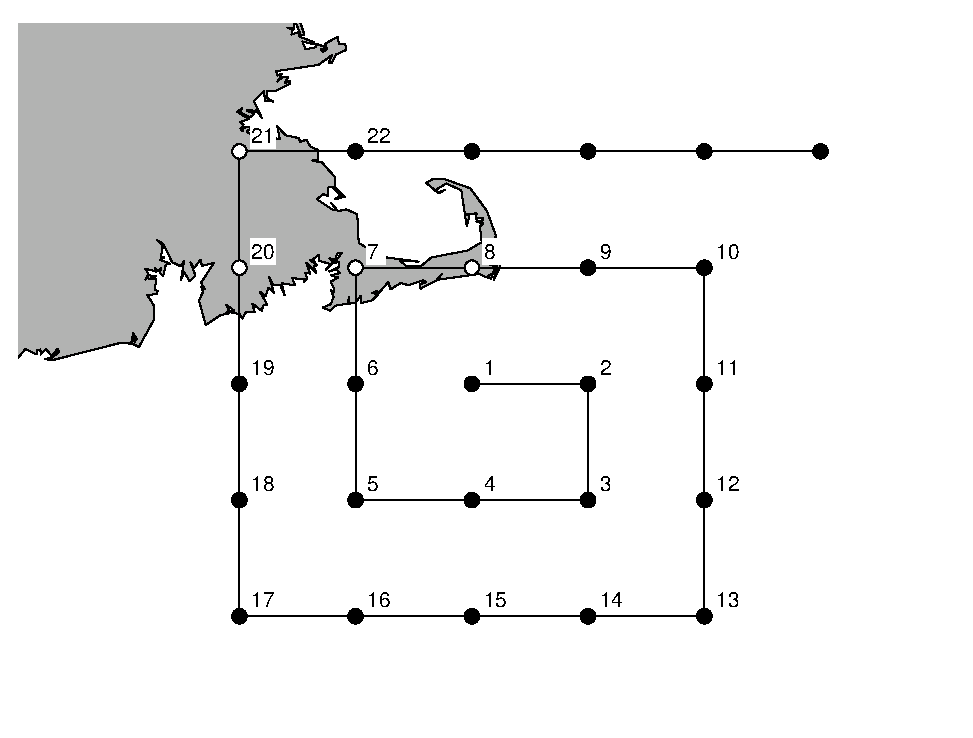
\epsfig{file=./num/wavetrack.eps,width=3.5in}
\caption{含陆地（阴影）的近岸规则计算网格上的追踪螺旋示例。黑点表示活动网格点，白点表示非活动（干）网格点。}
         \label{fig:wavetrack} \botline
\end{center}
\end{figure}

\begin{equation}
    GoF_{i} = {\left( \frac{T_\mathrm{p} - \tilde{T}^\mathrm{n}_{\mathrm{p},i}}{\Delta T_\mathrm{n}} \right)}^2 + 
                     {\left( \frac{\theta_\mathrm{p} - \tilde{\theta}^\mathrm{n}_{\mathrm{p},i}}{\Delta\theta_\mathrm{n}} \right)}^2 +
                     {\left( \frac{H_\mathrm{m0} - \tilde{H}^\mathrm{n}_{\mathrm{m0},i}}{\Delta H_\mathrm{n}} \right)}^2\ \ ,
\label{eq:grdgof}
\end{equation} 

\noindent
其中 $\Delta T_\mathrm{n}$、$\Delta\theta_\mathrm{n}$ 和 $\Delta
H_\mathrm{n}$ 是合并判据 \citep{art:WHD13}。若对于最接近匹配，式~(\ref{eq:grdgof}) 右端前两项中任一项超过 1，则认为差异过大，并将一个新的波系分配给该分区。这里，相邻点搜索范围设为 1，因此最多可找到四个此前已关联的相邻点（例如位置 15 会有此前处理过的相邻点 3、4、5 和 14）。在某些情况下，需要迭代合并。

下一步是在时间上对这些波系进行相关。当前时间层 $t$ 的每个系统 $i$ 与上一时间层 $(t-1)$ 的系统 $j$ 中最接近的匹配相关联。该过程中考虑波系的三个特征，即：(i) 系统内的空间平均峰值波周期 $\tilde{T}^\mathrm{s}_{\mathrm{p},t,i}$，其中
$\mathrm{s}$ 表示系统平均；(ii) 空间平均峰值波向
$\tilde{\theta}^\mathrm{s}_{\mathrm{p},t,i}$；以及 (iii) 两个系统在地理空间中重叠的网格点数 $\cap_{i,j}$。这些特征组合形成以下 GoF 函数：

\begin{equation}
    GoF_{i,j} = {\left( \frac{\tilde{T}^\mathrm{s}_{\mathrm{p},t,i} - \tilde{T}^\mathrm{s}_{\mathrm{p},t-1,j}}{\Delta T_\mathrm{s}} \right)}^2 + 
                       {\left( \frac{\tilde{\theta}^\mathrm{s}_{\mathrm{p},t,i} - \tilde{\theta}^\mathrm{s}_{\mathrm{p},t-1,j}}{\Delta\theta_\mathrm{s}} \right)}^2 +
                       {\left( \frac{N_{t-1,j} - \cap_{i,j}}{0.5N_{t-1,j}} \right)}^2\ \ ,
\label{eq:timegof}
\end{equation} 

\noindent
其中 $\Delta T_\mathrm{s}$ 和 $\Delta\theta_\mathrm{s}$ 是合并判据，$N$ 是一个系统中的网格点总数，见 \cite{art:WHD13}。为使追踪过程聚焦于波场中的高能区域，每个系统的空间平均周期和峰值方向值都按有效波高的平方加权。当前时间层 $t$ 的系统 $i$ 被分配给上一时间层 $(t-1)$ 中使式~(\ref{eq:timegof}) 最小的系统 $j$。若对于使式~(\ref{eq:timegof}) 最小的系统，式~(\ref{eq:timegof}) 右端三项中任一项超过 1，则分配一个新的系统编号。对最后一项而言，这意味着最小空间重叠要求，此处任意设为 50\%。该项主要影响盆地尺度区域，因为此类区域中的系统通常小于计算区域。为提高稳健性，识别出的系统细节会保存五个时间层，之后释放系统关联。

\vssub
\subsection{~嵌套} \label{sub:num_nest}
\conthead{\ws}{H. L. Tolman}

\noindent
传统上，波浪模式只考虑单向嵌套，即由低分辨率网格向高分辨率网格提供边界数据。\ws{} 一直提供这种方法，相关内容见 \para\ref{sub:one_way}。在模式 3.14 版中，引入了多网格波浪模式驱动程序，考虑网格之间的完整双向嵌套。该方法见 \para\ref{sub:two_way}。下文图示考虑规则网格，但所讨论的原则同样适用于曲线网格和三角形网格。


% -------------------------------------------------------------
\vssub
\subsubsection{~传统单向嵌套} \label{sub:one_way}
\vssub

\begin{figure}
\begin{center}

\setlength{\unitlength}{0.001in}

\begin{picture}(3000,1800)(0,-1550)

\put(0200,-1200){\vector(1,0){2100}}
\put(2400,-1250){\makebox(400,100){\small 空间}}
\put(0300,-1300){\vector(0,1){1300}}
\put(0100, 0100){\makebox(400,100)[c]{\small 时间}}

\multiput(0300,-1200)(0,300){4}{\circle {50}}
\multiput(0600,-1200)(0,300){4}{\circle {50}}
\multiput(0900,-1200)(0,300){4}{\circle {50}}
\multiput(1200,-1200)(0,300){4}{\circle*{50}}
\multiput(1500,-1200)(0,300){4}{\circle {50}}
\multiput(1800,-1200)(0,300){4}{\circle {50}}
\multiput(2100,-1200)(0,300){4}{\circle {50}}

\put(0300,-0150){\makebox(600,100)[c]{“陆地”}}
\put(0900,-0200){\vector(-1,0){575}}

\put(1500,-0150){\makebox(600,100)[c]{海洋}}
\put(1500,-0200){\vector(1,0){875}}
				       
\put(0900, 0050){\makebox(600,100)[c]{边界数据}}
\put(1100,-1200){\dashbox{50}(0200,1150){}}

\put(1050,-1550){\makebox(600,100)[c]{边界格式}}
\put(1200,-1400){\dashbox{25}(0300,1100){}}

\put(1550,-0750){\makebox(600,100)[l]{内部格式}}
\put(1500,-0800){\vector(1,0){875}}

\end{picture}
\end{center}

\caption{{\file ww3\_shel} 中使用的传统单向嵌套方法。空间和时间上的一维表示，符号表示网格点。} \label{fig:nest1}
\botline
\end{figure}


常规波浪模式程序 {\file ww3\_shel} 考虑单个波浪模式网格。该程序包含将边界条件从大尺度运行传递到小尺度运行的选项。每次运行可同时接受一个边界条件数据集，并生成最多 9 个边界条件数据集。为在水深和流场不兼容时保证波能守恒，边界数据由能量谱 $F(\sigma,\theta)$ 组成。数据文件包含生成运行中网格点处的谱，以及在所请求边界点处插值谱所需的信息。因此，如果小尺度运行的输入点位于大尺度运行的网格线上，传输文件的大小就最小。作为输入使用时，谱会在每个全局时间步长 $\Delta t_g$ 上以谱分量线性插值的方式在空间和时间上插值。

在波浪模式中包含边界数据的数值方法如图~\ref{fig:nest1} 所示。活动边界点在网格中被指定，用于将海点与陆点或其他停用网格点分隔开。在活动边界点和海点之间，应用局地边界格式（通常为一阶）。在模式内部海点中，则使用所选传播格式。

传统单向嵌套方法的实际使用方面在附录~\ref{app:nest} 中有更详细讨论。


% -------------------------------------------------------------
\vssub
\subsubsection{~双向嵌套} \label{sub:two_way}
\vssub

模式 3.14 版包含在程序 {\file ww3\_multi} 中使用多网格或镶嵌方法进行波浪建模的选项 \citep{tol:Vict06a,
  tol:MMAB07b, tol:OMOD08b}。在该程序中，可考虑任意数量、任意分辨率的网格，并在每个相关模式时间步长上在网格之间交换数据。网格被赋予等级编号，较低等级对应较低分辨率，相同等级对应相近分辨率（但不一定完全相同）。网格之间考虑三类数据传输：

\begin{itemize}
\item 从低等级网格向高等级网格传输数据。
\item 从高等级网格向低等级网格传输数据。
\item 在相同等级网格之间传输数据。
\end{itemize}

从低等级网格向高等级网格传输数据，是通过向高等级网格提供边界数据来完成的，方式与上一节和图~\ref{fig:nest1} 中所述的传统单向嵌套方法相同。

\begin{figure}
\begin{center}

\setlength{\unitlength}{0.001in}

\begin{picture}(3000,1900)(0,-1600)

\multiput(0300,-1400)(0,300){6}{\circle {50}}
\multiput(0600,-1400)(0,300){6}{\circle {50}}
\multiput(0900,-1400)(0,300){6}{\circle {50}}
\multiput(1200,-1400)(0,300){6}{\circle {50}}
\multiput(1500,-1400)(0,300){6}{\circle {50}}
\multiput(1800,-1400)(0,300){6}{\circle {50}}
\multiput(2100,-1400)(0,300){6}{\circle {50}}
\multiput(2400,-1400)(0,300){6}{\circle {50}}
\multiput(2700,-1400)(0,300){6}{\circle {50}}

\multiput(0450,-1550)(300,0){8}{\dashbox{50}(0000,1800){}}
\multiput(0150,-1250)(0,300){5}{\dashbox{50}(2700,0000){}}

\multiput(0400,-1450)(0,800){3}{\circle*{100}}
\multiput(1400,-1450)(0,800){3}{\circle*{100}}
\multiput(2400,-1450)(0,800){3}{\circle*{100}}

\put(895,-1055){\framebox(1010,810){}}
\put(900,-1050){\framebox(1000,800){}}
\put(905,-1045){\framebox(990,790){}}

\end{picture}
\end{center}

\caption{双向嵌套方法中协调低等级网格与高等级网格的概念示意。$\circ$ 和虚线分别表示高等级网格点和网格单元，$\bullet$ 和实线分别表示低等级网格及其中心网格单元。}
\label{fig:nest2}
\botline
\end{figure}


当该方法与从高等级到低等级的数据传输结合时，就建立了完整的双向嵌套方法。在 {\file ww3\_multi} 中，当高等级网格在时间上“追上”低等级网格之后，会将低等级网格中的数据与高等级网格中的数据相协调。考虑到低等级网格的分辨率按定义低于高等级网格的分辨率，从高等级网格中的能量 $E_{h,j}$ 估计低等级网格中的波能 $E_{l,i}$ 的一种自然方式为

\begin{equation}
E_{l,i} = \sum w_{i,j} E_{h,j} \:\:\: , \label{eq:nest_hg1}
\end{equation}

\noindent
其中 $i$ 和 $j$ 是两个网格中的网格计数器，$w_{i,j}$ 是平均权重。权重可按与波能守恒一致的方式定义为：高等级网格中覆盖低等级网格单元 $i$ 的网格单元 $j$ 的面积，并用低等级网格单元 $i$ 的面积归一化。图~\ref{fig:nest2} 对此作了说明。为避免循环协调，低等级网格中为高等级网格提供边界数据的网格点不以这种方式更新。

\input{zh/num/fig_nest3_zh}

相同等级的重叠网格不能使用上述双向嵌套技术来一致地交换数据。相反，所有这类网格都先传播一个时间步长，随后如图~\ref{fig:nest3} 所示对网格进行协调。对于网格 1（图~\ref{fig:nest3} 中的 $\circ$），可区分两个区域。在区域 C 中，自上次协调以来，边界影响已传播进入网格。实际穿透深度取决于数值格式的模板宽度以及传播时间步数。在区域 A 和 B 中，来自边界的信息尚未穿透，因此该区域可视为网格 1 的“内部”。类似地，区域 A 表示网格 2（图~\ref{fig:nest3} 中的 $\bullet$）的边界穿透深度，而 B 和 C 表示网格 2 的内部。网格 1 和网格 2 之间一种简单且一致的协调方法，是在区域 A 中仅使用网格 1 的数据（必要时将网格 1 的数据插值到网格 2 的网格点），并在区域 C 中仅使用网格 2 的数据。在区域 B 中，两个网格的内部部分重叠，可通过使用两个网格的加权平均获得一致解。注意，该方法很容易扩展到多个重叠网格。

注意，对于显式数值传播格式，以及具有相同分辨率且网格点重合的重叠网格，只要重叠区域足够宽，重叠网格的解就可以与兼容的单一网格解相同。

\vspace{\baselineskip} 
\noindent 
{\file ww3\_multi} 中的双向嵌套技术在很大程度上是自动化的。每个网格都独立准备，并具有自己首选的时间步进信息。每个网格期望从低等级网格获得边界数据的位置，会像单向嵌套方法一样标记。实现双向嵌套技术所需的所有其他簿记操作都是自动化的，不过可能需要若干次迭代，以确保每个网格中定义的所有输入边界点都能从多网格应用中的其他网格获得边界数据。作为替代，每个网格也可像传统嵌套方法一样从外部数据文件获取数据。在当前实现中，每个网格必须从单个文件或从多网格应用中的其他网格获得全部边界数据，但不能同时从文件和网格接收数据。关于为同时运行所有网格而开发的管理算法，详见 \citet[section 3.4]{tol:MMAB07b} 和 \cite{tol:OMOD08b}，此处不再重复。

注意，{\file ww3\_multi} 中使用的网格不需要具有相同的谱离散。谱会在 {\file
ww3\_multi} 中即时转换。该方法所用数值技术的细节可见 \citet[section 3.5.5]{tol:MMAB07b}。在这种方法中生成多网格可能很繁琐，并且需要保证网格之间的一致性以获得一致的模式结果。因此，\cite{tol:MMAB07a, tol:OMOD08a} 开发了自动网格生成工具。


\section{~波浪模型结构与数据流} \label{chapt:run}
\newcounters

% 本章正文正按 \input 文件逐节替换为中文；表格字段和程序名需保留代码语义。
\vsssub
\subsection{~程序设计} \label{run:design}
\vssub

\ws{} 的核心是波浪模式子程序，它可由独立程序壳调用，也可由任何需要动态更新波浪数据的其他程序调用。\ws{} 发布包提供了两个这样的程序（例如 {\code ww3\_shel} 和 {\code ww3\_multi}）。辅助程序包括网格预处理器 {\code ww3\_grid}、用于生成人工初始条件的程序 {\code ww3\_strt}、用于单个 {\code ww3\_shel} 或多网格 {\code ww3\_multi} 应用的通用程序壳、两个输入预处理器（{\code ww3\_prep} 和 {\code ww3\_prnc}），以及用于网格输出数据（{\code ww3\_outf} 和 {\code ww3\_ounf}）和点输出数据（{\code ww3\_outp} 和 {\code ww3\_ounp}）的后处理器。

在本节中，文件名用 {\file file} 字体表示，文件内容用 {\code code} 字体表示，{\sc fortran} 程序元素用 {\F fortran} 字体表示。主波浪模式子程序为 {\F w3wave}。除多网格波浪模式 {\file ww3\_multi} 外，数据文件均以文件扩展名 {\file .ww3} 标识；在 {\file ww3\_multi} 中，文件扩展名标识所选多网格镶嵌中的各个网格。为简单起见，本章统一使用文件扩展名 {\file .ww3}。

包含基本数据流的关系图见图~\ref{fig:run_elements}。该图展示了一个典型工作流，如下所述。网格预处理器 {\code ww3\_grid} 写出模式定义文件 {\file mod\_def.ww3}，其中包含海底和障碍物信息，以及定义物理和数值方法的参数值。波浪模式可采用冷启动或热启动。热启动需要重启动文件 {\file restart.ww3}，该文件可由波浪模式在前一次运行中创建，也可由初始条件程序 {\code ww3\_strt} 创建。若重启动文件不可用，波浪模式将自动初始化。若打开线性增长或谱播种，模式可从平静海面（$H_s=0$）开始；否则初始条件将由基于初始风场的参数化有限风区谱组成（见初始条件程序中的相应选项）。

波浪模式例程（{\F w3wave}）可选地生成最多 9 个重启动文件 {\file restart{\em{n}}.ww3}，其中 {\file{\em{n}}} 表示一位整数。对于望远镜式嵌套应用，波浪模式还可选地从文件 {\file nest.ww3} 读取边界条件，并在 {\file nest{\em{n}}.ww3} 中为后续嵌套运行生成边界条件。此外，模式会将原始数据转储到输出文件 {\file out\_grd.ww3}、{\file out\_pnt.ww3}、{\file track\_o.ww3} 和 {\file partition.ww3}（分别为网格平均波浪参数、指定位置处的谱、沿轨迹的谱和分区波浪数据）。需输出谱的轨迹定义在文件 {\file track\_i.ww3} 中。注意，波浪模式不写标准输出，因为当 \ws{} 作为集成模式的一部分时这样会不方便。相反，它维护自己的日志文件 {\file log.ww3}，并可选地为共享内存版本输出测试文件 {\file test.ww3}，或为分布式内存版本输出 {\file test{\em{nnn}}.ww3}，其中 {\em nnn} 是从 1 开始的处理器编号。最后，还提供多种输出后处理器（原始网格场、点输出和轨迹输出文件的二进制后处理；波浪数据的 NetCDF 和 GRIB(2) 打包；用于后续 GrADS 图形处理的网格和谱数据后处理）。下文给出了所有程序元素及其输入文件的更详细说明。注意，每个例程的源代码都有完整文档。这些文档是关于 \ws{} 的额外信息来源。

\input{zh/run/fig_flow_zh}

\ws{} 专用文件在程序子例程中按名称打开。不过，单元号由用户\footnote{~{\file ww3\_multi} 除外。} 在每个 {\file \.inp} 中定义，从而保证在集成模式中实现时具有最大的灵活性。

除波浪模式子程序外，还提供初始化例程和用于数据同化的接口例程。该例程包含一个通用接口，可提供执行完整谱数据同化所需的所有模式组件。该例程集成在通用波浪模式壳中，该壳可为带或不带数据同化的波浪模式执行时间步管理。程序壳还提供一种简单而灵活的方式，将多种数据提供给数据同化方案。数据同化尚未包含在多网格波浪模式壳中。

\vssub
\subsection{~波浪模式例程} \label{sec:core}
\vssub

波浪模式驱动器是 \ws{} 框架包中的一个子程序。要运行该模式驱动子程序，需要一个程序壳。\ws{} 提供了一个简单的独立壳，见 \para\ref{sec:ww3shel}，也提供了一个更复杂的多网格模式壳，见 \para\ref{sec:ww3multi}。本节重点介绍波浪模式驱动子程序。

波浪模式初始化例程 {\F w3init} 对单个波浪模式网格执行模式初始化。这包括：通过定义单元号来建立部分 I/O 系统；初始化内部时间管理；处理模式定义文件（{\file mod\_def.ww3}）；处理初始条件（{\file restart.ww3}）；准备模式输出；以及计算依赖网格的参数。若模式为 \mpi{} 环境编译，则会确定并初始化计算和输出所需的全部通信（模式全程使用持久 \mpi{} 通信）。

在初始化完成后，可任意多次调用波浪模式例程 {\F w3wave}，以推进单个网格上的波场随时间演变。在若干初始检查之后，该子程序会插值风和流、更新冰浓度和水位、传播波场，并在若干时间步上应用所选源项。内部时间步由需要执行计算的时间区间以及请求的输出时刻共同定义。计算结束时，该例程向调用程序提供所请求的波浪数据场。{\F w3wave} 接口的文档可在源代码（{\file w3wavemd.ftn}）中找到。

\input{zh/run/fig_log_zh.tex} 

除上述原始数据文件外，程序还维护一个日志文件 {\file log.ww3}。该文件由 {\F w3init} 打开（{\F w3init} 包含在 {\file w3wavemd.ftn} 的 {\F w3wave} 中），并向该文件写入若干自解释的头部信息。对 {\F w3wave} 的每次后续调用都会在该日志文件的“动作表”中增加数行，如图~\ref{fig:log} 所示。标识为 `step' 的列显示所考虑的离散时间步。标识为 `pass' 的列给出调用 {\F w3wave} 的序列号；例如 3 表示该动作发生在第三次调用 {\F w3wave} 中。第三列显示该时间步的结束时间。输入和输出列显示模式的相应动作。{\tt X} 表示输入已更新或输出已执行。{\tt F} 表示首次读取场，{\tt L} 表示最后一次输出。七个输入列分别表示边界条件（{\tt b}）、风场（{\tt w}）、水位（{\tt l}）、流场（{\tt c}）、冰浓度（{\tt i}）以及同化数据（{\tt d}）。注意，数据同化发生在波浪例程调用之后、时间步末端。七个输出列分别表示网格输出（{\tt g}）、点输出（{\tt p}）、沿轨迹输出（{\tt t}）、重启动文件（{\tt r}）、边界数据（{\tt b}）、分区谱数据（{\tt f}）以及耦合输出（{\tt c}）。

对于多网格波浪模式 \citep[][{\file ww3\_multi}]{tol:OMOD08b}，在基本波浪模式例程周围构建了一组例程。三个主要例程是初始化例程 {\F wminit}、时间步进例程 {\F wmwave} 和终止例程 {\F wmfinl}，其功能与上述单网格例程类似。注意，原始输入和输出文件会针对镶嵌中的各个网格分别生成，并通过将标准文件扩展名 `{\file .ww3}' 替换为用户在 {\file ww3\_grid.inp} 文件中为每个单独网格选择的唯一标识符来识别。每个单独网格都维护日志文件，同时也维护一个总日志文件 {\file log.mww3}。

\vssub
\subsection{~数据同化接口} \label{sec:das}
\vssub

如上所述，波浪模式子程序还配有一个数据同化接口例程（{\file w3wdasmd.ftn} 中的 {\F w3wdas}）。该例程集成在独立壳中（见 \para\ref{sec:ww3shel}），用于为组合的波浪模式/数据同化方案提供时间步管理。它尚未集成到多网格模式驱动器中，尽管多网格模式管理算法已经考虑了它。

这里假定采用一种相当简单的方法：数据同化在选定时刻执行，而波浪模式持续向前积分。在程序壳的设置中，数据同化在模式到达目标时间之后、尚未产生输出之前执行。完成数据同化后，只为按请求生成输出而再次调用波浪模式例程。因此，给定时刻的波浪模式输出将包含该目标时刻数据同化的影响。

通用程序壳还处理若干类型的待同化数据，并将其传递给数据同化接口例程。所有数据都需要使用波浪模式输入预处理器进行预处理（见 \para\ref{sec:ww3prep}），并由通用壳通过文件名识别。目前最多可使用三个不同的数据文件。暂定而言，它们可分别为平均波浪参数、一维谱数据和二维谱数据。不过，这并未硬编码到模式中，实际上需要由用户定义。

目前尚无可用的数据同化软件包。因此，需要用户提供数据同化方案，并可使用接口例程（{\file w3wdasmd.ftn} 中的 {\F w3wdas}）将其纳入波浪模式；该例程的文档应足以支持必要的编程。关于如何将用户提供的软件添加到 \ws{} 编译系统，详见下一章。虽然 NCEP 目前正在研究波浪数据同化技术，但没有计划将波浪数据同化软件作为 \ws{} 软件包的一部分发布。

\vssub
\subsection{~辅助程序} \label{sec:auxprog}

\vsssub
\subsubsection{一般概念}
\vsssub

除轨迹输出后处理器外，这里介绍的所有辅助程序都从预定义输入文件读取输入。该文件的内容决定每个辅助程序的用户选择。注释行可用用户确定的字符表示，规则如下：输入文件第一行的第一个字符将被视为注释字符，用于在整个输入文件中标识注释行。该注释字符必须出现在输入行的第一列才有效。在以下各节的所有示例中，第一行的第一个字符为 `{\tt \$}'。因此，所有以 `{\tt \$}' 开头的行都只包含注释，不会被解析到辅助程序中。按照标准，所有辅助程序都会将格式化输出写到标准输出单元。

以下各节使用示例输入文件描述所有可用辅助程序。这些示例文件位于 \ws{} 软件包的 {\code inp} 目录中。每个示例输入文件内都包含用户可激活的全部可能选项，其中大多数以 `{\tt \$}' 开头作为注释行。本节中的文件反映示例文件的实际内容。以下各节还显示与所示输入文件相关联的可执行程序名称、程序名（如 program 语句中所示）、源代码文件，以及输入和输出文件及其单元号（在文件名后的括号中）。标有 \opt{} 的输入和输出文件为可选文件。下文提到的中间文件均为 {\F unformatted} 文件，此处不详细说明。每个文件均由单个例程写入和读取，并给出相应例程以供查阅更多文档。

\begin{list}{}{\itemsep 0mm \parsep 0mm \leftmargin 40mm \labelwidth 30mm}
\item[{mod\_def.ww3} \hfill] 子程序 {\F w3iogr}（{\file w3iogrmd.ftn}）。
\item[{out\_grd.ww3} \hfill] 子程序 {\F w3iogo}（{\file w3iogomd.ftn}）。
\item[{out\_pnt.ww3} \hfill] 子程序 {\F w3iopo}（{\file w3iopomd.ftn}）。
\item[{track\_o.ww3} \hfill] 子程序 {\F w3iotr}（{\file w3iotrmd.ftn}）。
\item[{restart.ww3}  \hfill] 子程序 {\F w3iors}（{\file w3iorsmd.ftn}）。
\item[{nest.ww3}     \hfill] 子程序 {\F w3iobc}（{\file w3iobcmd.ftn}）。
\item[{partition.ww3}\hfill] 子程序 {\F w3iosf}（{\file w3iosfmd.ftn}）。
\end{list}

\noindent
程序的预处理和编译将在后续两章讨论。源代码中提供了模式测试运行示例。

\vsssub
\subsubsection{配置文件}
\vsssub

这里介绍的所有辅助程序都从 namelist 文件（新形式）或输入文件（传统形式）读取参数和配置。虽然大多数辅助程序提供 namelist 文件选项，但仍有一些程序只能使用传统输入文件形式。后一类程序的 namelist 文件将在未来公开发布版中提供。对于已经使用 namelist 的程序，模板文件存放在 model/nml 目录中。也可以使用 model/aux/bash 目录中存放的 {\code bash} 工具，将传统 {\file inp} 文件转换为新的 {\file nml} 格式。若运行目录中同时存在 {\file inp} 和 {\file nml} 文件，则优先使用 namelist 文件。对于回归测试，默认行为是所有程序都使用 {\file inp} 文件运行；若要改用 {\file nml} 文件，必须添加 -N 选项。一些新功能仅在 namelist 中可用，未来开发也将主要面向 namelist 使用。

专用于某一程序的 namelist 配置文件提供了更易读且适应性更强的文件。一个 {\file nml} 文件包含一个或多个 namelist，每个参数都有默认值，并可由用户定义值覆盖。nml 文件中 namelist 的定义没有强制顺序。namelist 以 `{\tt \&SOMETHING\_NML}' 开始，以 `{\tt /}' 结束。若 namelist 文件跳过某一节，则会使用全部默认值。当程序读取其 namelist 文件时，所有 namelist 的默认值和用户定义值都会输出到日志文件中，以提高可追踪性。

读取程序配置的传统方式来自预定义输入文件。输入文件第一行的第一个字符将被视为注释字符，用于标识输入文件中的注释行。该注释字符必须位于输入行的第一列才有效。在以下各节的所有示例中，以 `{\tt \$}' 开头的行因此只包含注释。所有程序还会将格式化输出写到标准输出单元。

\vspace{\baselineskip} \noindent
下面给出一个 {\file inp} 文件片段及其对应的 {\file nml} 文件片段：

\vspace{\baselineskip} \noindent
\rule[1mm]{43mm}{.5mm} {\rm 示例输入文件开始（传统形式）}
\rule[1mm]{43mm}{.5mm}
\begin{footnotesize}
\begin{verbatim}
$ -------------------------------------------------------------------- $
$ WAVEWATCH III Grid preprocessor input file                           $
$ -------------------------------------------------------------------- $
$ Grid name (C*30, in quotes)
$
  'TEST GRID (GULF OF NOWHERE)   '
$
$ Frequency increment factor and first frequency (Hz) ---------------- $
$ number of frequencies (wavenumbers) and directions, relative offset
$ of first direction in terms of the directional increment [-0.5,0.5].
$ In versions 1.18 and 2.22 of the model this value was by definiton 0,
$ it is added to mitigate the GSE for a first order scheme. Note that
$ this factor is IGNORED in the print plots in ww3_outp.
$
   1.1  0.04118  32  24  0.
$
\end{verbatim}
\end{footnotesize}
\rule[1mm]{46mm}{.5mm} 示例输入文件结束（传统形式）
\rule[1mm]{45.1mm}{.5mm}

\vspace{\baselineskip} \noindent
\rule[1mm]{43mm}{.5mm} {\rm 示例输入文件开始（namelist 形式）}
\rule[1mm]{43mm}{.5mm}
\begin{footnotesize}
\begin{verbatim}
! -------------------------------------------------------------------- !
! WAVEWATCH III - ww3_grid.nml - Grid pre-processing                   !
! -------------------------------------------------------------------- !


! -------------------------------------------------------------------- !
! Define the spectrum parameterization via SPECTRUM_NML namelist
!
! * namelist must be terminated with /
! * definitions & defaults:
!     SPECTRUM%XFR   = 0.  ! frequency increment
!     SPECTRUM%FREQ1 = 0.  ! first frequency (Hz)
!     SPECTRUM%NK    = 0   ! number of frequencies (wavenumbers)
!     SPECTRUM%NTH   = 0   ! number of direction bins
!     SPECTRUM%THOFF = 0.  ! relative offset of first direction [-0.5,0.5]
! -------------------------------------------------------------------- !
&SPECTRUM_NML
  SPECTRUM%XFR           =  1.1
  SPECTRUM%FREQ1         =  0.04118
  SPECTRUM%NK            =  32
  SPECTRUM%NTH           =  24
/
\end{verbatim}
\end{footnotesize}
\rule[1mm]{46mm}{.5mm} 示例输入文件结束（namelist 形式）
\rule[1mm]{45.1mm}{.5mm}



\pb

\vsssub
\subsubsection{网格预处理器} \label{sub:ww3grid}
\vsssub

\proddefH{ww3\_grid}{w3grid}{ww3\_grid.ftn}
\proddeff{输入}{ww3\_grid.nml}{Namelist 配置文件。}{10} (App.~\ref{sec:config012})
\proddefa{ww3\_grid.inp}{传统配置文件。}{10} (App.~\ref{sec:config011})
\proddefa{'grid file' \opt}{包含海底水深的文件。}{user}
\proddefa{'obstr. file' \opt}{包含子网格障碍物的文件。}{user}
\proddefa{'mask file' \opt}{包含网格掩膜的文件。}{user}
\proddeff{输出}{standard out}{程序的格式化输出。}{6}
\proddefa{mod\_def.ww3}{\ws{} 格式的模式定义文件。}{20}
\proddefa{mask.ww3 \opt}{陆海掩膜文件（开关 {\F o2}a）。}{20}
\proddeff{暂存}{ww3\_grid.scratch}{格式化暂存文件。}{90}

\vspace{\baselineskip} \noindent
注意，海底和障碍物数据可位于同一文件中。

\pb

\vsssub
\subsubsection{初始条件程序} \label{sub:ww3strt}
\vsssub

\proddefH{ww3\_strt}{w3strt}{ww3\_strt.ftn}
\proddeff{输入}{ww3\_strt.inp}{传统配置文件。}{10} (App.~\ref{sec:config021})
\proddefa{mod\_def.ww3}{模式定义文件。}{20}
\proddeff{输出}{standard out}{程序的格式化输出。}{6}
\proddefa{restart.ww3}{\ws{} 格式的重启动文件。}{20}

\pb

\vsssub
\subsubsection{边界条件程序} \label{sub:ww3bound}
\vsssub

\proddefH{ww3\_bound}{w3bound}{ww3\_bound.ftn}
\proddeff{输入}{ww3\_bound.inp}{传统配置文件。}{10} (App.~\ref{sec:config031})
\proddefa{mod\_def.ww3}{模式定义文件。}{20}
\proddefa{'spectra file' \opt}{包含波谱的文件。}{user}
\proddeff{输出}{standard out}{程序的格式化输出。}{6}
\proddefa{nest.ww3}{边界条件文件。}{33}

\vspace{\baselineskip} \noindent
注意：当使用该程序为旋转极点网格上的模式生成边界输入时，输入谱始终假定为在标准极点上定义。

\pb

\vsssub
\subsubsection{NetCDF 边界条件程序} \label{sub:ww3bounc}
\vsssub

\proddefH{ww3\_bounc}{w3bounc}{ww3\_bounc.ftn}
\proddeff{输入}{ww3\_bounc.nml}{Namelist 配置文件。}{10} (App.~\ref{sec:config042})
\proddefa{ww3\_bounc.inp}{传统配置文件。}{10} (App.~\ref{sec:config041})
\proddefa{mod\_def.ww3}{模式定义文件。}{20}
\proddefa{'spectra file' \opt}{NetCDF 格式的波谱文件。}{user}
\proddeff{输出}{standard out}{程序的格式化输出。}{6}
\proddefa{nest.ww3}{边界条件文件。}{33}

\vspace{\baselineskip} \noindent
注意：当使用该程序为旋转极点网格上的模式生成边界输入时，输入谱始终假定为在标准极点上定义。

\pb

\vsssub
\subsubsection{输入场预处理器} \label{sec:ww3prep}
\vsssub

\proddefH{ww3\_prep}{w3prep}{ww3\_prep.ftn}
\proddeff{输入}{ww3\_prep.inp}{传统配置文件。}{10} (App.~\ref{sec:config051})
\proddefa{mod\_def.ww3}{模式定义文件。}{11}
\proddefa{'user input'\opt}{见下文示例。}{user}
\proddeff{输出}{standard out}{程序的格式化输出。}{6}
\proddefa{level.ww3\opt}{水位文件。}{12}
\proddefa{current.ww3\opt}{流场文件。}{12}
\proddefa{wind.ww3\opt}{风场文件。}{12}
\proddefa{ice.ww3\opt}{冰场文件。}{12}
\proddefa{data0.ww3\opt}{同化数据（`mean'）。}{12}
\proddefa{data1.ww3\opt}{同化数据（`1-D spectra'）。}{12}
\proddefa{data2.ww3\opt}{同化数据（`2-D spectra'）。}{12}

\vspace{\baselineskip} 
\vspace{\baselineskip} 

\noindent 
注意，可选输出文件专用于 {\file ww3\_shel} 和
{\file ww3\_multi}，但实际波浪模式例程不会处理这些文件。因此，如果波浪模式例程在其他程序壳或集成程序中使用，则不需要这些文件。不过，读写这些文件的例程与系统无关，因此可用于基本波浪模式的定制应用。这些文件的读写由子程序 {\F w3fldg}
（{\file w3fldsmd.ftn}）执行。关于更多文档和文件格式，请参考该例程。
\pb

\vsssub
\subsubsection{NetCDF 输入场预处理器} \label{sec:ww3prnc}
\vsssub

\proddefH{ww3\_prnc}{w3prnc}{ww3\_prnc.ftn}
\proddeff{输入}{ww3\_prnc.nml}{Namelist 配置文件。}{10} (App.~\ref{sec:config062})
\proddefa{ww3\_prnc.inp}{传统配置文件。}{10} (App.~\ref{sec:config061})
\proddefa{mod\_def.ww3}{模式定义文件。}{11}
\proddefa{'user input'\opt}{见下文示例。}{user}
\proddeff{输出}{standard out}{程序的格式化输出。}{6}
\proddefa{level.ww3\opt}{水位文件。}{12}
\proddefa{current.ww3\opt}{流场文件。}{12}
\proddefa{wind.ww3\opt}{风场文件。}{12}
\proddefa{ice.ww3\opt}{冰场文件。}{12}
\proddefa{data0.ww3\opt}{同化数据（`mean'）。}{12}
\proddefa{data1.ww3\opt}{同化数据（`1-D spectra'）。}{12}
\proddefa{data2.ww3\opt}{同化数据（`2-D spectra'）。}{12}

\vspace{\baselineskip} 
\vspace{\baselineskip} 
\noindent 
关于可在定制程序中用于打包输入文件的工具，见上一节（\ref{sec:ww3prep}）末尾的说明。

\pb

\vsssub
\subsubsection{潮汐预报程序} \label{sub:ww3prtide}
\vsssub

\proddefH{ww3\_prtide}{w3tide}{ww3\_prtide.ftn}
\proddeff{输入}{ww3\_prtide.inp}{传统配置文件。}{10} (App.~\ref{sec:config071})
\proddefa{mod\_def.ww3}{模式定义文件。}{20}
\proddefa{current.ww3\_tide or level.ww3\_tide}{包含潮汐分潮的文件。}{user}
\proddeff{输出}{standard out}{程序的格式化输出。}{6}
\proddefa{current.ww3 or level.ww3}{水位或流强迫。}{33}

\vspace{\baselineskip} 
\vspace{\baselineskip} 
\noindent 
用户提供的文件 current.ww3\_tide 或 level.ww3\_tide 是二进制文件，可通过使用 'AT' 选项运行 ww3\_prnc 获得，然后将所得文件 current.ww3 或 level.ww3 重命名为 current.ww3\_tide 或 level.ww3\_tide。用于潮汐预报的潮汐分潮可以是这些文件中已有分潮的一个子集，也可以是全部分潮。

由于干湿变化或网格不匹配，在某些 \ws{} 节点上，潮汐分潮可能错误或缺失。可通过对特定分量设置最大振幅来检测错误分潮。当振幅超过这些最大值时，将从最近节点外推潮汐分潮。该功能仅在三角形网格上测试过。

\pb

\vsssub
\subsubsection{通用壳程序} \label{sec:ww3shel}
\vsssub

\proddefH{ww3\_shel}{w3shel}{ww3\_shel.ftn}
\proddeff{输入}{ww3\_shel.nml}{Namelist 配置文件。}{10} (App.~\ref{sec:config082})
\proddefa{ww3\_shel.inp}{传统配置文件。}{10} (App.~\ref{sec:config081})
\proddefa{mod\_def.ww3}{模式定义文件。}{30}
\proddefa{restart.ww3}{重启动文件。}{30}
\proddefa{nest.ww3\opt}{边界条件文件。}{33}
\proddefa{level.ww3\opt}{水位文件。}{11}
\proddefa{current.ww3\opt}{流场文件。}{12}
\proddefa{wind.ww3\opt}{风场文件。}{13}
\proddefa{ice.ww3\opt}{冰场文件。}{14}
\proddefa{data0.ww3\opt}{同化数据。}{15}
\proddefa{data1.ww3\opt}{同化数据。}{16}
\proddefa{data2.ww3\opt}{同化数据。}{17}
\proddefa{track\_i.ww3\opt}{输出轨迹信息。}{22}
\proddeff{输出}{standard out}{程序的格式化输出。}{6}
\proddefa{log.ww3}{波浪模式的输出日志（见 \para\ref{sec:core}）。}{20}
\proddefa{test.ww3\opt}{波浪模式的测试输出。}{6/21}
\proddefa{restart{\sl{n}}.ww3\opt}{重启动文件。}{30}
\proddefa{nest{\sl{n}}.ww3\opt}{嵌套文件。}{34-42}
\proddefa{out\_grd.ww3\opt}{网格场原始输出。}{31}
\proddefa{out\_pnt.ww3\opt}{谱的原始输出。}{32}
\proddefa{track\_o.ww3\opt}{沿轨迹谱的原始输出。}{23}
\proddeff{暂存}{ww3\_shel.scratch}{格式化暂存文件。}{90}

\pb

\vsssub
\subsubsection{ww3\_multi 的自动网格拆分 (ww3\_gspl)} \label{sub:ww3gspl}
\vsssub

\proddefH{ww3\_gspl}{w3gspl}{ww3\_gspl.ftn}
\proddeff{输入}{ww3\_gspl.inp}{传统配置文件。}{10} (App.~\ref{sec:config091})
\proddefa{mod\_def.{\it xxx}}{待拆分网格的模式定义文件。}{11}
\proddeff{输出}{standard out}{程序的格式化输出。}{6}
\proddefa{{\it xxx}.bot}{子网格的水深文件。}{11}
\proddefa{{\it xxx}.obst}{子网格的障碍物文件。}{11}
\proddefa{{\it xxx}.mask}{子网格的掩膜文件。}{11}
\proddefa{{\it xxx}.tmpl}{子网格的 {\file ww3\_grid.inp}。}{11}
\proddefa{ww3\_multi.{\it xxx}.{\it n}}{需要修改的 {\file
ww3\_multi.inp} 部分模板。}{11}
\proddefa{ww3.ww3\_gspl}{包含子网格地图的 GrADS 文件（使用开关 {\F o16}）。}{35}
\proddefa{ww3.ctl}{GrADS 地图控制文件（{\F o16}）。}{35}

\vspace{\baselineskip} 
\noindent 
为进一步自动化网格拆分，提供了脚本 {\file ww3\_gspl.sh}。该脚本运行 {\file ww3\_gspl}，随后为所有子网格生成 {\file mod\_def} 文件。若提供了文件 {\file ww3\_multi.inp}，该文件也会被更新。脚本的工作方式可通过命令行标志 {\file -h} 显示，其输出如图~\ref{fig:gspl} 所示。

\pb

\begin{figure}[t]
{\scriptsize \input{ww3_gspl.sh.out} }
\caption{通过命令行选项 {\file -h} 运行 {\file ww3\_gspl.sh} 得到的选项说明。} \label{fig:gspl}
%\botline
\end{figure}


\clearpage

\vsssub
\subsubsection{多网格壳程序} \label{sec:ww3multi}
\vsssub

\proddefH{ww3\_multi}{w3mlti}{ww3\_multi.ftn}
\proddeff{输入}{ww3\_multi.nml}{Namelist 配置文件。}{8} (App.~\ref{sec:config102})
\proddefa{ww3\_multi.inp}{传统配置文件。}{8} (App.~\ref{sec:config101})
\proddeff{输出}{standard out}{程序的格式化输出。}{6}
\proddefa{log.mww3}{波浪模式驱动器的输出日志。}{9}
\proddefa{test.mww3\opt}{波浪模式的测试输出。}{auto}

\vspace{\baselineskip}
\noindent
该波浪模式程序需要并产生大量输入和输出文件，这些文件与 \para\ref{sec:ww3shel} 中 {\file ww3\_shel} 的文件一致；其中，文件扩展名 {\file .ww3} 会替换为特定网格的标识符。注意，所有文件均按名称打开，单元号分配是动态且自动的。

为使所有现有功能可用，现已有一个使用 namelist 的新版输入文件。这是未来将支持的版本，因为它可更灵活地添加新功能。{\bf 请注意，4.8.2 之前版本的 GCC 编译器不支持 namelist 形式。}

\pb

\vsssub
\subsubsection{网格整合} \label{sub:ww3gint}
\vsssub
\proddefH{ww3\_gint}{w3gint}{ww3\_gint.ftn}
\proddeff{输入}{ww3\_gint.inp}{传统配置文件。}{10} (App.~\ref{sec:config111})
\proddefa{mod\_def.*}{基准网格和目标网格的 \ws{} 格式模式定义文件}{20}
\proddefa{out\_grd.*}{基准网格的 \ws{} 格式网格场文件}{30+}
\proddeff{输出}{standard out}{程序的格式化输出。}{6}
\proddefa{out\_grd.*}{目标网格的 \ws{} 格式网格场文件}{30+}

\vspace{\baselineskip}
\noindent
该后处理程序从若干重叠网格获取场数据，并生成统一的输出文件。不同的模式定义文件和场输出文件由与每个特定网格关联的唯一标识符识别。目前，该程序适用于曲线网格和直角网格。程序会写出一个权重文件 {\file WHTGRIDINT.bin}；在后续使用相同源网格和目标网格的运行中可读取该文件，从而在输入网格数量较多和/或目标网格分辨率较高时节省大量时间。

\vspace{\baselineskip}
\noindent
网格整合程序可使用线性插值或最近邻插值。当分区输出用于谱重构时，建议使用后者。线性插值会导致分区扩散，从而产生虚假的能量线并人为增加总能量。
\vspace{\baselineskip}
\vspace{\baselineskip}
\noindent
注意，该程序可与网格拆分程序 {\file ww3\_gspl} 配合使用，并且 {\file ww3\_gspl.sh} 提供了为该程序生成模板输入文件的选项（见 \para\ref{sub:ww3gspl}）。

\pb

\vsssub
\subsubsection{网格输出后处理器} \label{sec:ww3outf}
\vsssub

\proddefH{ww3\_outf}{w3outf}{ww3\_outf.ftn}
\proddeff{输入}{ww3\_outf.inp}{传统配置文件。}{10} (App.~\ref{sec:config121})
\proddefa{mod\_def.ww3}{模式定义文件。}{20}
\proddefa{out\_grd.ww3}{原始网格输出数据。}{20}
\proddeff{输出}{standard out}{程序的格式化输出。}{6}
\proddefa{\ldots \opt}{传输文件。}{50}

\vspace{\baselineskip} 
\noindent
对于 {\F itype = 3}，传输文件的文件名扩展名用于标识该文件的内容。各数据类型对应的文件扩展名见第~\pageref{tab:fields} 页表~\ref{tab:fields}。

\pb

\vsssub
\subsubsection{网格输出 NetCDF 后处理器} \label{sec:ww3ounf}
\vsssub

\proddefH{ww3\_ounf}{w3ounf}{ww3\_ounf.ftn}
\proddeff{输入}{ww3\_ounf.nml}{Namelist 配置文件。}{10} (App.~\ref{sec:config132})
\proddefa{ww3\_ounf.inp}{传统配置文件。}{10} (App.~\ref{sec:config131})
\proddefa{mod\_def.ww3}{模式定义文件。}{20}
\proddefa{out\_grd.ww3}{原始网格输出数据。}{20}
\proddefa{NC\_globatt.inp}{附加全局属性（已弃用）}{994}
\proddefa{ounfmeta.inp}{用户定义的元数据属性}{60}
\proddeff{输出}{standard out}{程序的格式化输出。}{6}
\proddefa{\opt  .nc}{NetCDF 文件}{}


\vspace{\baselineskip}

\noindent
当文件中只放入一个场时，每种数据类型对应的缩写场名（来自 ww3\_outf 的文件扩展名）见第~\pageref{tab:fields} 页表~\ref{tab:fields}。

\noindent
\paragraph{元数据的用户配置：}

\noindent
默认元数据（属性）会为每个 WW3 输出变量生成到输出 netCDF 文件中。如有需要，用户可通过名为 `ounfmeta.inp' 的输入文本文件覆盖已有元数据，或配置额外元数据。


\noindent
`ounfmeta.inp' 文件可用于覆盖或配置以下内容：
\begin{itemize}
  \item 修改/扩展网格输出变量的 netCDF 属性。
  \item 修改/扩展“全局”netCDF 属性。
  \item 定义/重新定义坐标参考系统。
  \item 定义用于为分区参数输出变量生成属性的模板字符串。
\end{itemize}

\noindent
ounfmeta.inp 文件中的条目通过带有关键字标记的\emph{节}给出。空行和注释行（以 \texttt{\$} 开头）会被忽略。注意：所有关键字和 `Field Name ID' 字符串（例如 \texttt{HS}）均不区分大小写。所有 netCDF 属性名区分大小写。

\noindent
\paragraph{修改/添加 WW3 网格输出场的属性：}

\noindent
输出场通过 META 关键字选择，其后可跟整数对 \texttt{GroupNum} 和 \texttt{ParamNum}，也可跟 \texttt{FldTag} 字符串；这些值对应于 ww3\_shel.nml 或 ww3\_shel.inp 中的 `Output field parameter definitions table'。任一种形式后面都可跟一个可选整数值 \texttt{IFC}，用于在多分量场中选择分量（例如 WND 和 CUR 输出场中的 U、V 分量）。

\begin{verbatim}
  META  <GroupNum ParamNum>  |  <FldTag>  [IFC]
    attr_name  = attr_value
    attr_name  = attr_value
    extra_attr = extra_value [type]
    extra_attr = extra_value [type]
  ... repeated as many times as required.
\end{verbatim}


\noindent
每个 \texttt{attr\_name} 对应一个已有变量属性，可以是以下属性之一（括号中给出替代内部名称）：
\begin{itemize}
 \item  \texttt{standard\_name (varns)} [string]：CF 标准名称。
 \item  \texttt{long\_name (varnl)} [string]：描述性长名称。
 \item  \texttt{globwave\_name (varng)} [string]：可选 GlobWAVE 名称。
 \item  \texttt{direction\_reference} 或 \texttt{dir\_ref (varnd)} [string]：方向场的可选参考框架。
 \item  \texttt{comment (varnc)} [string]：可选注释。
 \item  \texttt{units} [string]：场的单位。
 \item  \texttt{valid\_min (vmin)} [float]：数据的最小有效值。
 \item  \texttt{valid\_max (vmax)} [float]：数据的最大有效值。
 \item  \texttt{scale\_factor (fsc)} [float]：数据缩放因子，仅当变量类型为 SHORT 时使用。
\end{itemize}

\noindent
任何其他属性名均被认为是可选的“额外”属性。该额外属性可带有可选的 `type' 关键字，用于指定元数据的变量类型。若未提供类型，则默认为字符类型。有效类型为 \texttt{[c, r, i]} 之一，分别表示字符/字符串、实数/浮点或整数值。注意：以空格分隔的字符串额外字段应加引号。

\noindent
\paragraph{修改“全局”元数据：}

\noindent
全局元数据（即与文件关联，而非与某个特定变量关联）可用特殊的 \texttt{META global} 关键字组合指定：

\begin{verbatim}
  META global [nodefault]
    extra_attr = extra_value [type]
    extra_attr = extra_value [type]
\end{verbatim}

\noindent
可选关键字 \texttt{nodefault} 会抑制默认 WW3 全局元数据的输出。

\noindent
\paragraph{修改/定义坐标参考系统：}


\noindent
可用 \texttt{CRS} 关键字为所有网格输出场指定“坐标参考系统”（CRS）。至少必须指定 \texttt{grid\_mapping\_name} 属性。若定义了 CRS 节，所有输出场都会添加一个 \texttt{grid\_mapping} 属性，引用 CRS 变量。\texttt{crs\_vaname} 将在输出文件中创建为一个标量 NF90\_CHAR 变量。

\begin{verbatim}
  CRS <crs_varname>
    grid_mapping_name = <mapping name>
    attr = value
    attr = value
\end{verbatim}

\noindent
对于普通经纬度网格和旋转极点网格，ww3\_ounf 会生成合适的坐标参考系统，但可使用 CRS 关键字覆盖。


\noindent
\paragraph{分区参数模板字符串}

\noindent
分区输出的元数据指定方式略有不同；一个元数据条目用于某一场的所有分区。元数据通过\emph{模板字符串}针对特定分区编号专门化。内置模板字符串有两个：\texttt{SPART} 和 \texttt{IPART}。它们分别提供“字符串”描述（例如 `wind sea'、`primary swell' 等）或整数分区编号（1、2、3 等）。可在元数据属性值中用被 \texttt{< ... >} 包围的模板名引用它们，例如 \texttt{<SPART>}。

\noindent
也可以在 ounfmeta.inp 文件中用 \texttt{TEMPLATE} 关键字提供用户定义的分区参数模板字符串，如下所示：

\begin{verbatim}
  TEMPLATE <template-name>
    String for partition 0
    String for partition 1
    String for partition 2
    String for partition 3
    ... etc
\end{verbatim}

\noindent
若指定带有尾随下划线的 \texttt{<template-name>}，则会提供以下划线分隔（\texttt{\_}）而不是以空格分隔的字符串（这对 netCDF `standard name' 值很有用）。


\noindent
\paragraph{ounfmeta.inp 文件示例：}
\begin{verbatim}
   $ Lines starting with dollars are comments.
   $ The line starts a meta-data section for the depth field
   META DPT
     standard_name = depth
     long_name = "can be quoted string"
     comment = or an unquoted string
     vmax = 999.9

   $ Next one is HSig (group 2, field 1)
   META 2 1
     varns = "sig. wave height"
     varnl = "this is long name"

   $ Next one is second component of wind. It also sets an
   $ "extra" meta data value (height - a float)
   META WND 2
     standard_name = "v-wind"
     height = 10.0 "r"

   $ User defined partitioned parameters template strings:
   TEMPLATE PARTSTR
     wind wave
     primary swell
     secondary swell

   $ Use partition templates in partitioned Hs field:
   $ (SPART and IPART are built-in)
   META PHS
     standard_name = "<SPART_>_sigificant_wave_height"
     long_name = "<PARTSTR>"
     partition_number = "<IPART>"

   $ Coordinate reference system:
   CRS crs
     grid_mapping_name = "latitude_longitude"
     semi_major_axis = 6371000.0 f
     inverse_flattening = 0 f

   $ Global metadata:
   META global
     institution = UKMO
     comment "space seperated strings should be quoted" c
     version = 1.0 r

\end{verbatim}


\noindent
\paragraph{添加“forecast variables”：}
使用 ww3\_ounf.nml 输入文件时，可向输出 netCDF 文件添加可选辅助“forecast variables”（见 ww3\_ounf.nml）。当 \texttt{FCVARS = T} 时，将生成以下变量：
\begin{itemize}
 \item \texttt{forecast\_reference\_time}：与当前预报的“分析”关联的时间。对于跨多天拆分的文件很有用，因为它允许把某一特定时刻的预报追溯到其分析时间或起始时间。
 
 \item \texttt{forecast\_period}：自关联的 \texttt{forecast\_reference\_time} 起经过的时间段（单位为秒）。
\end{itemize}

\noindent
\texttt{forecast\_reference\_time} 默认为 ww3\_ounf.nml 中指定的 \texttt{TIMESTART}。不过，模式运行可能包含某种后报时段；在这种情况下，\texttt{forecast\_reference\_time} 应设置为合适的分析时间。此外，如果调用 ww3\_ounf 时使用的 \texttt{TIMESTART} 与模式起始时间不同，则需要显式指定正确的 \texttt{forecast\_reference\_time}，以确保 \texttt{forecast\_period} 计算正确。

\pb

\vsssub
\subsubsection{用于 GrADS 的网格输出后处理器} \label{sec:gxoutf}
\vsssub

\proddefH{gx\_outf}{gxoutf}{gx\_outf.ftn}
\proddeff{输入}{gx\_outf.inp}{传统配置文件。}{10} (App.~\ref{sec:config141})
\proddefa{mod\_def.ww3}{模式定义文件。}{20}
\proddefa{out\_grd.ww3}{原始网格输出数据。}{20}
\proddeff{输出}{standard out}{程序的格式化输出。}{6}
\proddefa{ww3.grads}{GrADS 数据文件。}{50}
\proddefa{ww3.ctl}{GrADS 控制文件。}{51}

\vspace{\baselineskip} 
\noindent 
该后处理器为 Grid Analysis and Display System \citep[GrADS,][]{man:GrADS} 生成包含网格模式参数的输入文件。
%This graphical software can be obtained from http://www.iges.org/grads.  -- website no longer valid
虽然 GrADS 也可处理 GRIB 文件，但当前预处理器更合适，因为该数据文件还可访问陆-海-冰地图。

\pb

\vsssub
\subsubsection{网格 GRIB 输出后处理器} \label{sec:ww3grib}
\vsssub

\proddefH{ww3\_grib}{w3grib}{ww3\_grib.ftn}
\proddeff{输入}{ww3\_grib.inp}{传统配置文件。}{10} (App.~\ref{sec:config151})
\proddefa{mod\_def.ww3}{模式定义文件。}{20}
\proddefa{out\_grd.ww3}{原始网格输出数据。}{20}
\proddeff{输出}{standard out}{程序的格式化输出。}{6}
\proddefa{gribfile}{GRIB 文件。}{50}

\vspace{\baselineskip} 
\noindent
该后处理器将平均波浪参数场打包为 GRIB 格式，可使用 GRIB version II 和 \ncep{} 的 w3 与 bacio 库例程，或使用 GRIB2 及 NCEP 的业务软件包。附加打包数据见第~\pageref{tab:fields} 页表~\ref{tab:fields}。

GRIB 打包使用 \ncep{} 的 GRIB 表，见 \cite{rep:GRIB1}。由于 w3 和 bacio 例程并非完全可移植，它们不随代码提供。用户必须提供相应例程。建议使用强制开关组中包含 `{\F nogrb}' 开关的附加 \ws{} 开关来激活这些例程，就像目前 \ncep{} 例程的情况一样。GRIB2 打包按照 \cite{rep:GRIB2} 执行，并使用 NCEP 的标准业务软件包。

表~\ref{tab:fields} 显示用于 GRIB 打包的 {\F kpds(5)} 数据值。对于分区数据，第一个数字表示风海，第二个数字表示涌浪。多数数据作为表面数据打包（{\F
kpds(6) = 0}）。不过，对于分区涌浪场，连续场会按连续层打包，层类型指示符设为（{\F
kpds(6) = 241}）。{\F kpds(7)} 标识实际层或涌浪场编号。

表~\ref{tab:fields} 还显示若干用于 GRIB2 打包的 {\F kpds} 数据值。表中第一个数字表示 {\F listsec0(2)}，用于标识 discipline 类型（例如海洋学、气象学等）。第二个数字表示 {\F kpds(1)}，用于标识该 discipline 类型内的参数类别（例如波浪、环流、海冰等）。第三个数字表示 {\F kpds(2)}，用于标识实际参数。对于分区数据，A/B 表示 A 用于风海、B 用于涌浪。此外，{\F kpds(10) = 0} 用于表面数据，{\F kpds(10) = 241 } 用于在连续层上打包连续涌浪场。{\F kpds(12)} 标识实际层或涌浪场编号。

尽管上述输入文件包含 \ws{} 全部 31 个输出场的标志，但并非所有场都可打包为 GRIB。如果选择了没有 GRIB 打包支持的参数，程序会向标准输出打印消息。表~\ref{tab:fields} 显示哪些参数可打包为 GRIB。注意，在 \ncep{}，从 GRIB 到 GRIB2 的转换与分区波浪模式输出的引入同时发生。这导致 GRIB 中出现一些重复定义，并导致 GRIB 和 GRIB2 打包之间出现一些表面上的不一致。

\pb

\vsssub
\subsubsection{点输出后处理器} \label{sec:ww3outp}
\vsssub

\proddefH{ww3\_outp}{w3outp}{ww3\_outp.ftn}
\proddeff{输入}{ww3\_outp.inp}{传统配置文件。}{10} (App.~\ref{sec:config161})
\proddefa{mod\_def.ww3}{模式定义文件。}{20}
\proddefa{out\_pnt.ww3}{原始点输出数据。}{20}
\proddefa{NC\_globatt.inp}{附加全局属性。}{994}
\proddeff{输出}{standard out}{程序的格式化输出。}{6}
\proddefa{tab{\sl{nn}}.ww3 \opt}{平均参数表，其中
{\file{\sl{nn}}} 为两位整数。}{\sl nn}
\proddefa{\ldots \opt}{传输文件。}{user}

\vspace{\baselineskip} 
\vspace{\baselineskip} 
\noindent 
在 \ws{} 早期版本中，谱公报使用由 {\F itype = 1} 和 {\F otype = 3} 生成的谱数据传输文件以及 {\file w3split} 程序（见 section~\ref{sec:install}）生成。这是一段即将淘汰的代码，此处仅为向后兼容而提供。该程序从标准输入读取以下五条记录（不允许注释行）：

\begin{list}{$\bullet$}{\itemsep 0mm \parsep 0mm}
\item 输出位置名称。
\item 表中使用的运行标识符。
\item 输入文件名称。
\item 标识 UNFORMATTED 输入文件的逻辑量。
\item 输出文件名称。
\end{list}

\noindent
以上所有字符串均以自由格式按字符读取，因此需要用引号括起。

\pb

\vsssub
\subsubsection{点输出 NetCDF 后处理器} \label{sec:ww3ounp}
\vsssub

\proddefH{ww3\_ounp}{w3ounp}{ww3\_ounp.ftn}
\proddeff{输入}{ww3\_ounp.nml}{Namelist 配置文件。}{10} (App.~\ref{sec:config172})
\proddefa{ww3\_ounp.inp}{传统配置文件。}{10} (App.~\ref{sec:config171})
\proddefa{mod\_def.ww3}{模式定义文件。}{20}
\proddefa{out\_pnt.ww3}{原始点输出数据。}{20}
\proddeff{输出}{standard out}{程序的格式化输出。}{6}
\proddefa{\ldots \opt}{传输文件。}{user}

\vspace{\baselineskip} 
\noindent 

\pb

\vsssub
\subsubsection{用于 GrADS 的点输出后处理器} \label{sec:gxoutp}
\vsssub

\proddefH{gx\_outp}{gxoutp}{gx\_outp.ftn}
\proddeff{输入}{gx\_outp.inp}{传统配置文件。}{10} (App.~\ref{sec:config181})
\proddefa{mod\_def.ww3}{模式定义文件。}{20}
\proddefa{out\_pnt.ww3}{原始点输出数据。}{20}
\proddeff{输出}{standard out}{程序的格式化输出。}{6}
\proddefa{ww3.spec.grads}{包含谱和源项的 GrADS 数据文件。}{30}
\proddefa{ww3.mean.grads}{包含平均波浪参数的文件。}{31}
\proddefa{ww3.spec.ctl}{GrADS 控制文件。}{32}

\vspace{\baselineskip} 
\noindent
该后处理器用于生成数据文件，使 GrADS（见上一节）能够绘制谱和源项的极坐标图。为实现这一点，谱和源项被存储为“经度-纬度”网格。对于每个输出点，会为数据生成不同名称，通常为 {\F
loc{\it nnn}}。当数据文件载入 GrADS 时，变量 {\F loc001} 将在第 1 层包含第一个请求输出点的谱网格，在第 2 层包含输入源项，依此类推。对于第二个输出点，数据存储在 {\F loc002} 中，依此类推。实际输出点名称通过控制文件 {\file ww3.spec.ctl} 传递给 GrADS。波高和环境数据从 {\file ww3.mean.grads} 获取。不过，用户无需了解 GrADS 数据文件和数据存储的细节。程序提供了 GrADS 脚本 {\file spec.gs}、{\file source.gs} 和 {\file 1source.gs}，用于从该后处理器的输出文件自动生成谱图。

注意：为使 GrADS 脚本正常工作，输出点名称不应包含空格。

\pb

\vsssub
\subsubsection{轨迹输出后处理器} \label{sec:ww3trck}
\vsssub

\proddefH{ww3\_trck}{w3trck}{ww3\_trck.ftn}
\proddeff{输入}{ww3\_trck.inp}{传统配置文件。}{10} (App.~\ref{sec:config191})
\proddefa{track\_o.ww3}{原始轨迹输出数据。}{11}
\proddeff{输出}{standard out}{程序的格式化输出。}{6}
\proddefa{track.ww3}{格式化数据文件。}{51}

\vspace{\baselineskip}
\noindent
该后处理器将原始轨迹输出数据转换为整数压缩的格式化文件。该文件包含以下头记录：

\begin{list}{$\bullet$}{\itemsep 0mm \parsep 0mm}
\item 文件标识符（长度为 34 的字符串）。
\item 频率数和方向数、第一个方向以及方向增量（弧度，海洋学约定）。
\item 每个频率箱的弧频率。
\item 对应的方向箱宽乘以频率箱宽，用于得到每个离散箱的能量。
\end{list}

\noindent
对于随时间和位置变化的每个输出点，将写出以下记录：
\begin{list}{$\bullet$}{\itemsep 0mm \parsep 0mm}
\item {\tt yyyymmdd hhmmss} 格式的日期和时间、以度为单位的经度和纬度，以及状态标识符
      `{\F ice}'、`{\F lnd}' 或 `{\F sea}'。以下两条记录仅对海点写出。
\item 以米为单位的水深，以米每秒为单位的海流和风的 $u$、$v$ 分量，
      以米每秒为单位的摩擦速度，以摄氏度为单位的气海温差，以及谱的缩放因子。
\item 以整数打包格式给出的完整谱（可用自由格式读取）。
\end{list}

\pb

\vsssub
\subsubsection{轨迹输出 NetCDF 后处理器} \label{sec:ww3trnc}
\vsssub

\proddefH{ww3\_trnc}{w3trnc}{ww3\_trnc.ftn}
\proddeff{输入}{ww3\_trnc.nml}{Namelist 配置文件。}{10} (App.~\ref{sec:config202})
\proddefa{ww3\_trnc.inp}{传统配置文件。}{10} (App.~\ref{sec:config201})
\proddefa{track\_o.ww3}{原始轨迹输出数据。}{11}
\proddeff{输出}{standard out}{程序的格式化输出。}{6}
\proddefa{*.nc}{NetCDF 文件。}{}

\vspace{\baselineskip}
\noindent
该后处理器将原始轨迹输出数据转换为 NetCDF 文件。输出 NetCDF 文件包含以下变量：

\begin{list}{$\bullet$}{\itemsep 0mm \parsep 0mm}
\item 自 1990-01-01 起算的天数形式的时间，即 UTC 时间下的儒略日。
\item 每个频率箱的频率（弧度）。
\item 每个频率箱下边带的频率（弧度）。
\item 每个频率箱上边带的频率（弧度）。
\item 每个频率箱的频率宽度（弧度）。
\item 每个方向箱的方向（海洋学约定）。
\item 沿时间维度给出的纬度和经度（度）。
\end{list}

\noindent
对于随时间和位置变化的每个输出点，将写出以下记录：
\begin{list}{$\bullet$}{\itemsep 0mm \parsep 0mm}
\item 轨迹名称（32 个字符）。
\item 完整谱（m2 s rad-1）。
\item 水深（m），海流和风的 $u$、$v$ 分量（m s-1），摩擦速度（m s-1），气海温差（摄氏度）。
\end{list}

\pb

\vsssub
\subsubsection{波浪系统的时空跟踪} \label{sec:ww3systrk}
\vsssub

\proddefH{ww3\_systrk}{w3systrk}{ww3\_systrk.ftn}
\proddeff{输入}{ww3\_systrk.inp}{传统配置文件。}{10} (App.~\ref{sec:config211})
\proddefa{partition.ww3}{谱分区文件。}{11}
\proddefa{sys\_restart.ww3\opt}{带系统记忆的重启动文件。}{12}
\proddefa{sys\_mask.ww3\opt}{掩膜文件。}{13}
\proddeff{输出}{sys\_log.ww3}{输出日志（并行运行时附加处理器编号）。}{20}
\proddefa{sys\_coord.ww3}{场的经纬度坐标。}{21}
\proddefa{sys\_hs.ww3}{各个波浪系统的有效波高场。}{22}
\proddefa{sys\_tp.ww3}{各个波浪系统的峰值周期场。}{23}
\proddefa{sys\_dir.ww3}{各个波浪系统的峰值方向场。}{24}
\proddefa{sys\_dspr.ww3}{各个波浪系统的方向扩展场。}{25}
\proddefa{sys\_pnt.ww3}{有效波高、峰值周期和峰值方向的点输出文件。}{26}
\proddefa{sys\_restart1.ww3}{重启动文件。}{27}
\proddefa{*.nc}{NetCDF 文件。}{ }

\vspace{\baselineskip}
\noindent
该程序目前仅实现于规则网格。时空跟踪基于谱分区数据文件进行。用于跟踪波浪系统的时间区间和地理区域都可以是分区文件所含数据的子集。组合参数 {\code dirKnob} 和 {\code perKnob} 用于影响地理空间中系统组合算法的严格程度，{\code dirTimeKnob} 和 {\code perTimeKnob} 则是在时间空间中的对应参数。较低的数值意味着更严格的判据，从而得到更小、数量更多的系统；这通常也会增加处理时间。上文给出了推荐值。这些值可以通过定义掩膜文件 {\file sys\_mask.ww3} 在局地进行调整，例如在岛屿周围。参数 {\code hsKnob} 和 {\code wetPts} 是低能量与小系统过滤器，即所有平均 $H_\mathrm{m0}$ 低于 {\code hsKnob} 的波浪系统，或尺寸小于整个区域大小的 {\code wetPts}*100\% 的波浪系统，都会被剔除。参数 {\code seedLat} 和 {\code seedLon} 影响波浪系统搜索螺旋的起点；默认值位于模式区域中心（由 {\code 0. 0.} 表示）。跟踪运行结束时，系统记忆的结束状态存储在 {\file sys\_restart1.ww3} 中。将该文件改名为 {\file sys\_restart.ww3} 后，可用于从先前的系统记忆状态重启动跟踪序列。

\pb

\vsssub
\subsubsection{重启动文件处理器} \label{sec:ww3uprstr}
\vsssub

\proddefH{ww3\_uprstr}{ww3uprstr}{ww3\_uprstr.ftn}
\proddeff{输入}{ww3\_uprstr.inp}{传统配置文件。}{10} (App.~\ref{sec:config221})
\proddefa{mod\_def.ww3}{模式定义文件。}{20}
\proddefa{restart.ww3}{重启动文件。}{ }
\proddefa{XXXX.grbtxt}{grbtxt 格式的有效波高分析文件。}{123}
\proddeff{输出}{restart001.ww3}{更新后的重启动文件。}{ }

\vspace{\baselineskip}

\paragraph{引言 \newline}

海面波浪场的大多数观测都是诊断变量有效波高（SWH）的观测。因此，波浪资料同化（WDA）常常在 SWH 空间中进行，随后需要把这些信息转换到预报变量空间，也就是波谱（WS），以便作为边界和/或初始条件（BIC）施加。

\subparagraph{\textbf{ww3\_uprstr} 的目的 \newline}
将 SWH 场分析中的能量重新分配到保存在重启动文件中的 WS 场。

\subparagraph{核心算法 \newline}
\textbf{ww3\_uprstr} 将背景谱的 SWH 设置为等于分析 SWH，并根据用户指定的谱形修改谱的形状。\textbf{ww3\_uprstr} 作为重启动读取器的扩展实现；它需要的输入包括重启动文件、分析 SWH，以及包含用户定义选项的 \textbf{ww3\_uprstr.inp}（见上文）。为减少即时计算，可能还需要额外文件。

\paragraph{如何使用 ww3\_uprstr \newline}
使用 \textbf{ww3\_uprstr} 时，用户需要遵循与所有 WAVEWATCH III 程序相同的逻辑。概括如下：

\begin{enumerate}
   \item \textbf{下载源代码} \newline
   从 6.07 版开始，\textbf{ww3\_uprstr} 源代码已经包含在 WAVEWATCH III 官方发布版中。
   \item \textbf{编译代码} \newline
   \textbf{ww3\_uprstr} 的编译方式与 WAVEWATCH III 的其他辅助程序相同，见手册中的相应章节。若需要调试输出，在 switch 文件中使用 \textbf{T} 标志。
   \item \textbf{测试可执行程序} \newline
   回归测试 \textbf{ww3\_ta1} 可用于测试 \textbf{ww3\_uprstr} 的不同选项。
   \item \textbf{运行 ww3\_uprstr} \newline
   运行 \textbf{ww3\_uprstr} 的步骤说明：
   \begin {description}
      \item{必需输入文件：\newline}
      \begin{itemize}
         \item \textbf{重启动文件。} 该文件由 WW3 在模式后报运行或前一循环中创建。预期文件名为 \textbf{restart.ww3}。
         \item \textbf{mod\_def.ww3}
         \item \textbf{ww3\_uprstr.inp。} 这是 \textbf{ww3\_uprstr} 的输入文件。用户必须定义：i. 同化日期；ii. 能量重新分配方法；iii. 取决于所选方法的百分比或输入文件。
         \item \textbf{分析输入文件。} 文件可以使用任意名称，但后缀决定用于导入数据的读取器。对大多数选项，读取器仅支持 \textbf{grbtxt} 格式。这是一个由 wgrib2 从分析 grib2 文件创建的文本文件，其结构如下：\newline

         \begin{tabular}{|c|}
            \hline
            NX NY       \\
            VAL0001     \\
            VAL0002     \\
            ...         \\
            VAL(NX*NY)  \\
            \hline
          \end{tabular}
    \newline
    \item 运行可执行程序：\newline
          \textgreater \$EXE/ww3\_uprstr \newline
          如果所有输入都准备正确，将创建新的重启动文件（\textbf{restart001.ww3}）。\textbf{ww3\_uprstr} 按与 restart.ww3 相同的格式导出更新后的谱。若要把它作为下一预报循环初始化的 BIC 使用，必须将其改名：\newline
          \textgreater mv \textbf{restart001.ww3} \textbf{restart.ww3}) \newline
          更新后的重启动文件随后即可按常规方式使用。
      \end{itemize}
   \end{description}

   \noindent\fbox{
      \parbox{\textwidth}{
         \textbf{提示}
         \begin{itemize}
            \item 重启动文件必须使用与 \textbf{ww3\_uprstr} 相同的 WW3 版本创建；该工具不提供向后兼容性。
            \item 在 \textbf{ww3\_uprstr.inp} 中定义的同化开始时间必须与重启动文件中的时间一致。
            \item 使用 \textbf{T} 时，\textbf{ww3\_uprstr.inp} 会导出背景重启动文件、分析以及更新后重启动文件中的 SWH 场。此外，更新前后的重启动文件谱也会作为文本文件导出。
         \end{itemize}
         }
   }
\end{enumerate}

\subparagraph{更新方法 \newline}
用户必须在 \textbf{ww3\_uprstr.inp} 中定义自己选择的更新算法。更新重启动文件的选项通过标志 UPD[N] 在 ww3\_uprstr.inp 中定义，其中 N 可以为 0F、0C、1、2 等。对于 N \textless 2 的 UPDN，同一修正应用于整个网格；预期输入为 PRCNTG，如 fac 所定义。对于 N \textgreater 1 的 UPDN，每个网格点都有自己的更新因子，输入为 grb2txt 格式。当前实现的更多细节见图~\ref{fig:uprstrflowchart}。

\begin{figure} \begin{center}
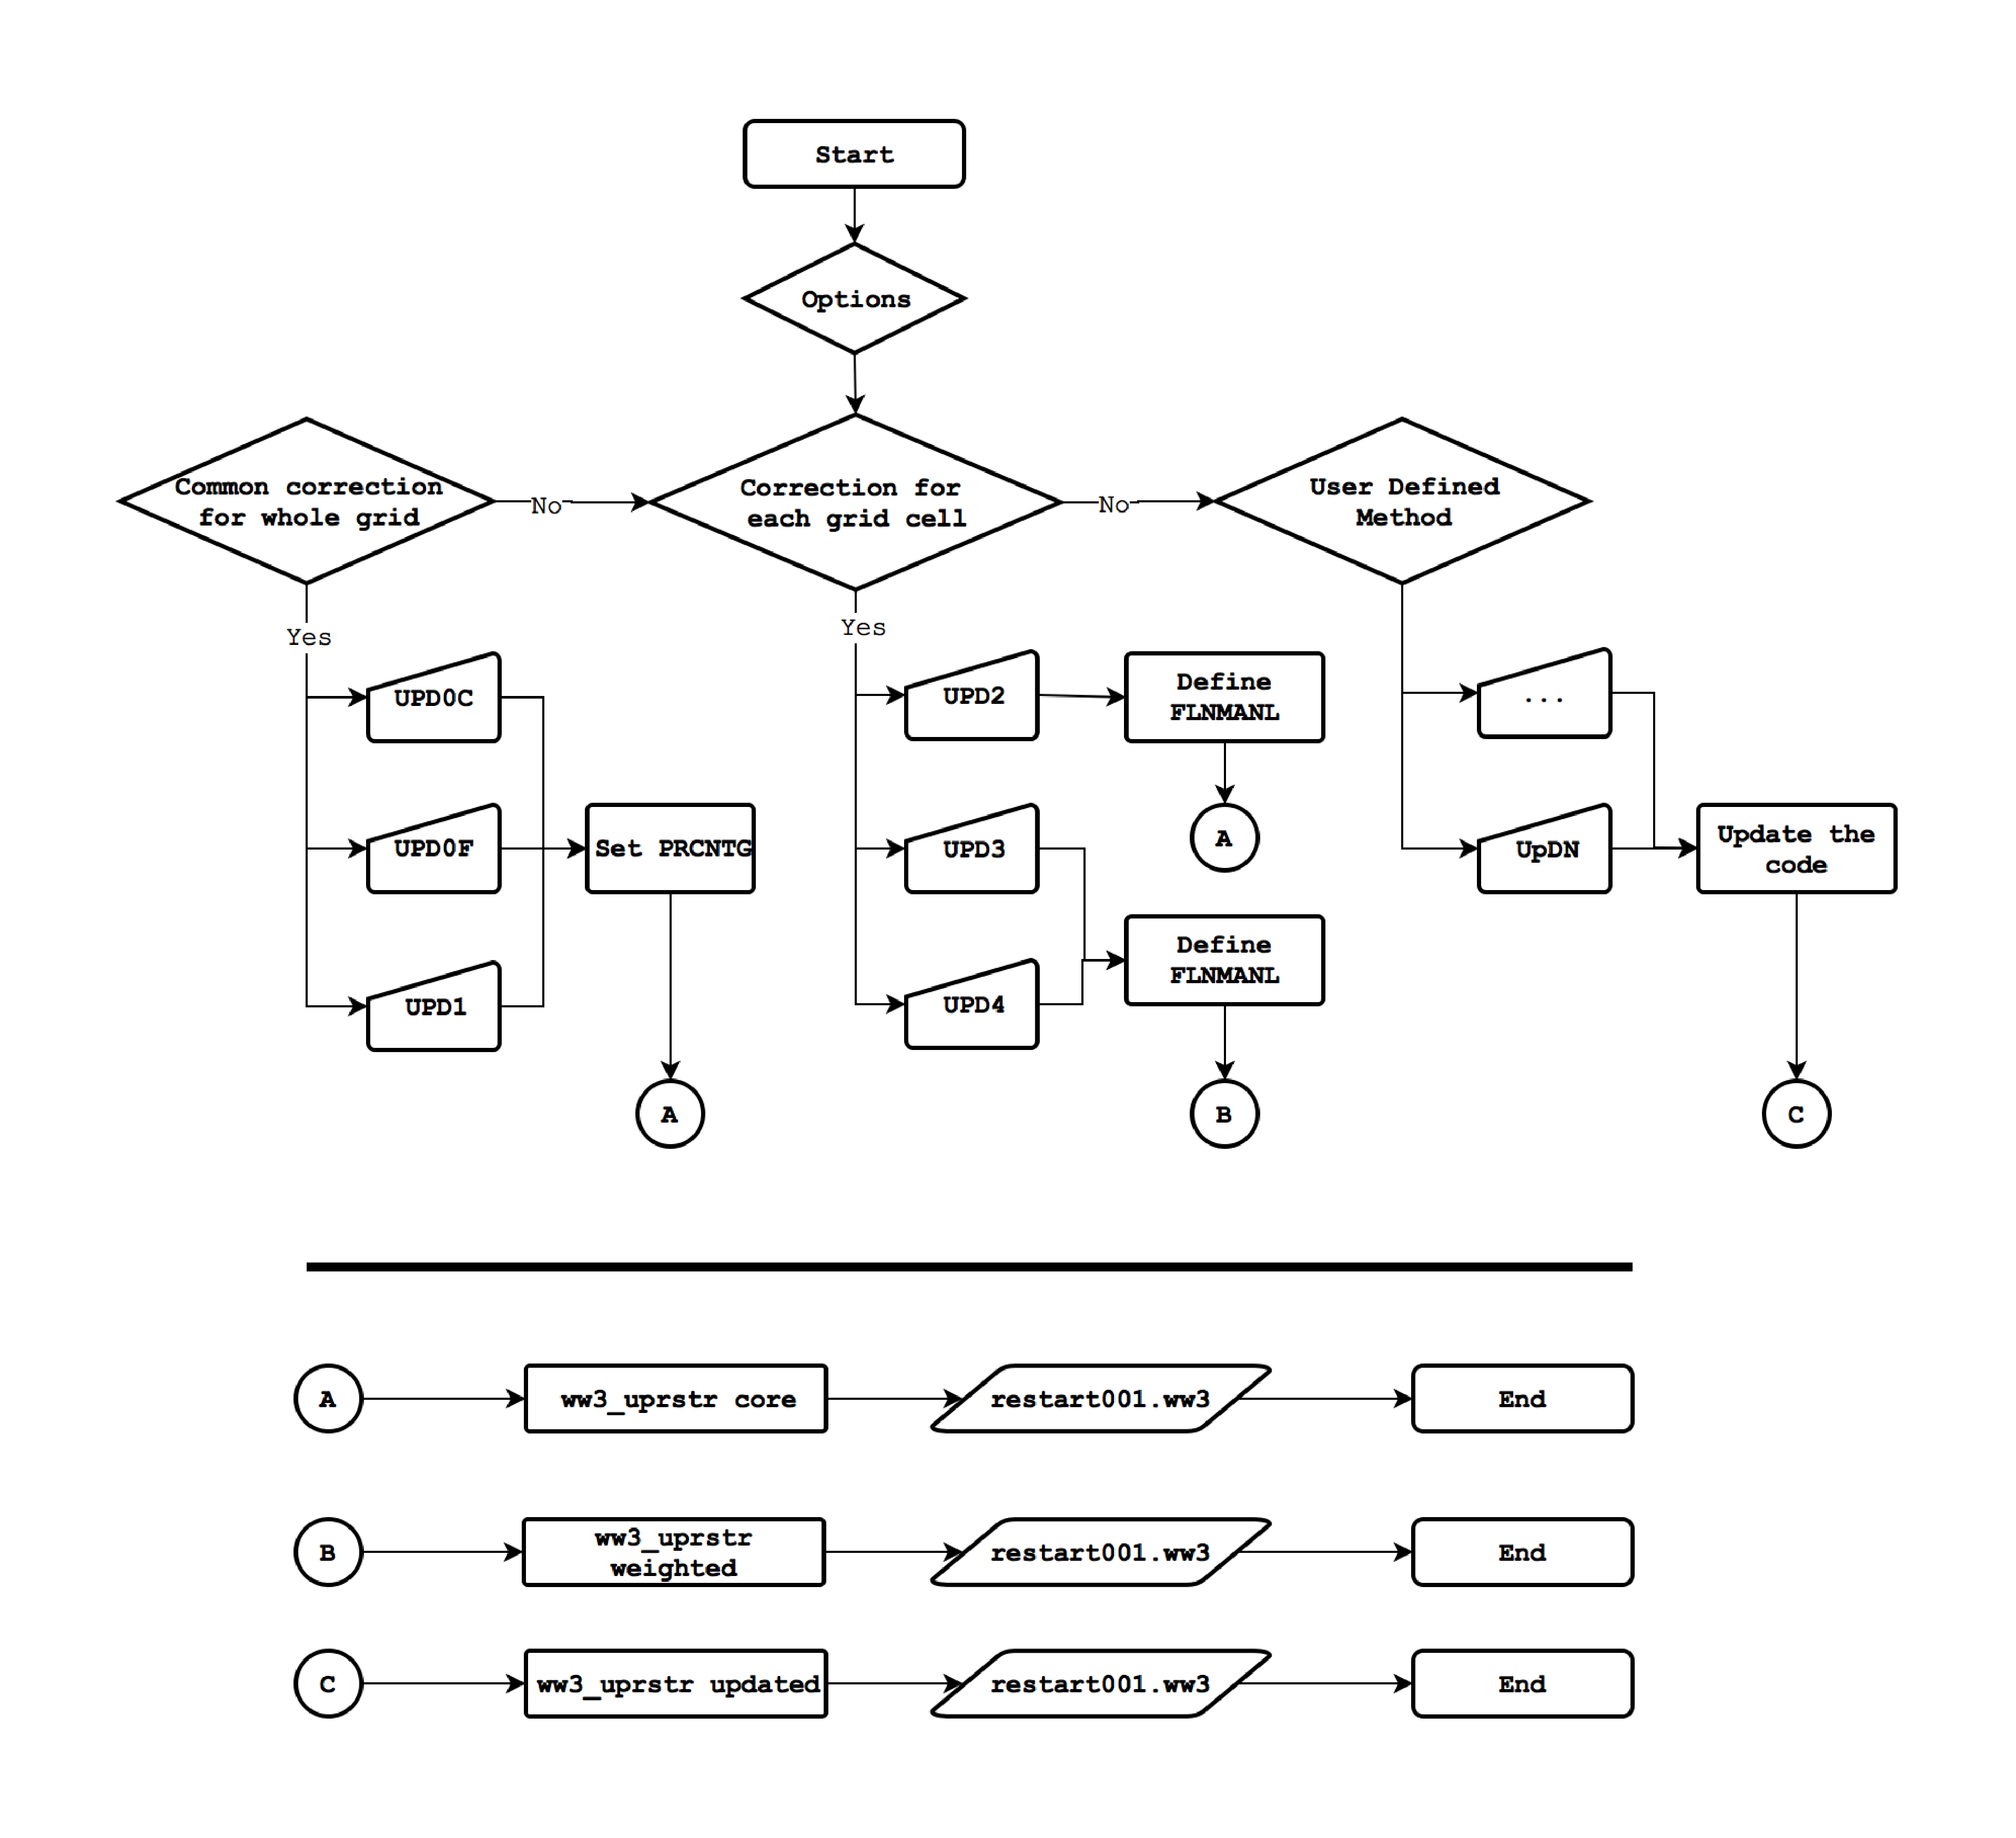
\includegraphics[width=0.9\textwidth]{./run/uprstr.eps}
\caption{WW3 重启动文件中波谱更新方法的实现流程图。可通过在 namelist 中增加 UPD 选项来实现其他方法。}
\label{fig:uprstrflowchart} \botline
\end{center}
\end{figure}

目前可用的 UPD 选项如下：
\begin{enumerate}
   \item UPD0C:: \textbf{自 5.16 版起已删除} 选项 0C，所有谱使用一个常数更新：\newline
      \(fac=(SWH\_Bckg-SWH\_Anl)/SWH\_Anl \).
   \item UPD0F:: 选项 0F，所有谱使用一个常数更新：\newline
      \(fac=SWH\_Anl/SWH\_Bckg \).
   \item UPD1 :: \textbf{自 5.16 版起已删除} 选项 1，fac(x,y,frq,theta) 按每个谱箱中的能量百分比加权；fac 与 UPDOF 相同。
   \item UPD2 :: 选项 2，根据 SWH\_Bckg 和 SWH\_Anl 在每个网格点计算 fac(x,y,frq,theta)。
   \item UPD3 :: 选项 3，更新因子是一个具有背景谱形状的曲面。
   \item UPD4 :: [当前版本未包含，仅保留位置] 选项 4，UPD3 的一般化。更新因子为多个曲面的和，这些曲面施加到背景谱上。该算法需要将每个分区映射到单个谱；该映射用于确定加权曲面。
   \item UPD5 :: 选项 5，修正按 UPD2 计算，但仅当风海为主导分量时才应用于谱的风海部分；否则修正整个谱。必需输入为分析 Hs 场，以及背景风速和风向。若要包含风数据，建议运行使用 WRST 开关构建的代码。
   \item UPD6 :: 选项 6，修正按 UPD5 计算，但风海分量还会使用 Toba (1973) 在频率空间中移动。必需输入为分析 Hs 场，以及背景风速和风向。若要包含风数据，建议运行使用 WRST 开关构建的代码。
\end{enumerate}

可以通过进一步扩展输入文件并向 \textbf{ww3\_uprstr.ftn} 添加源代码，加入其他用于将能量重新分配到 WS 并修正相关风场的方法。

\subparagraph{示例 \newline}
本节讨论一个最简单 WDA 应用的示例。图~\ref{fig:waveDAflowchart} 展示了 \textbf{ww3\_uprstr} 如何在一个简单波浪分析系统框架中使用。\newline

一次 WW3 运行（来自前一循环或来自后报）在适当时间提供 SWH 背景场以及对应的重启动文件。背景 SWH 场的格式必须与 WDA 模块输入兼容。

\begin{figure} \begin{center}
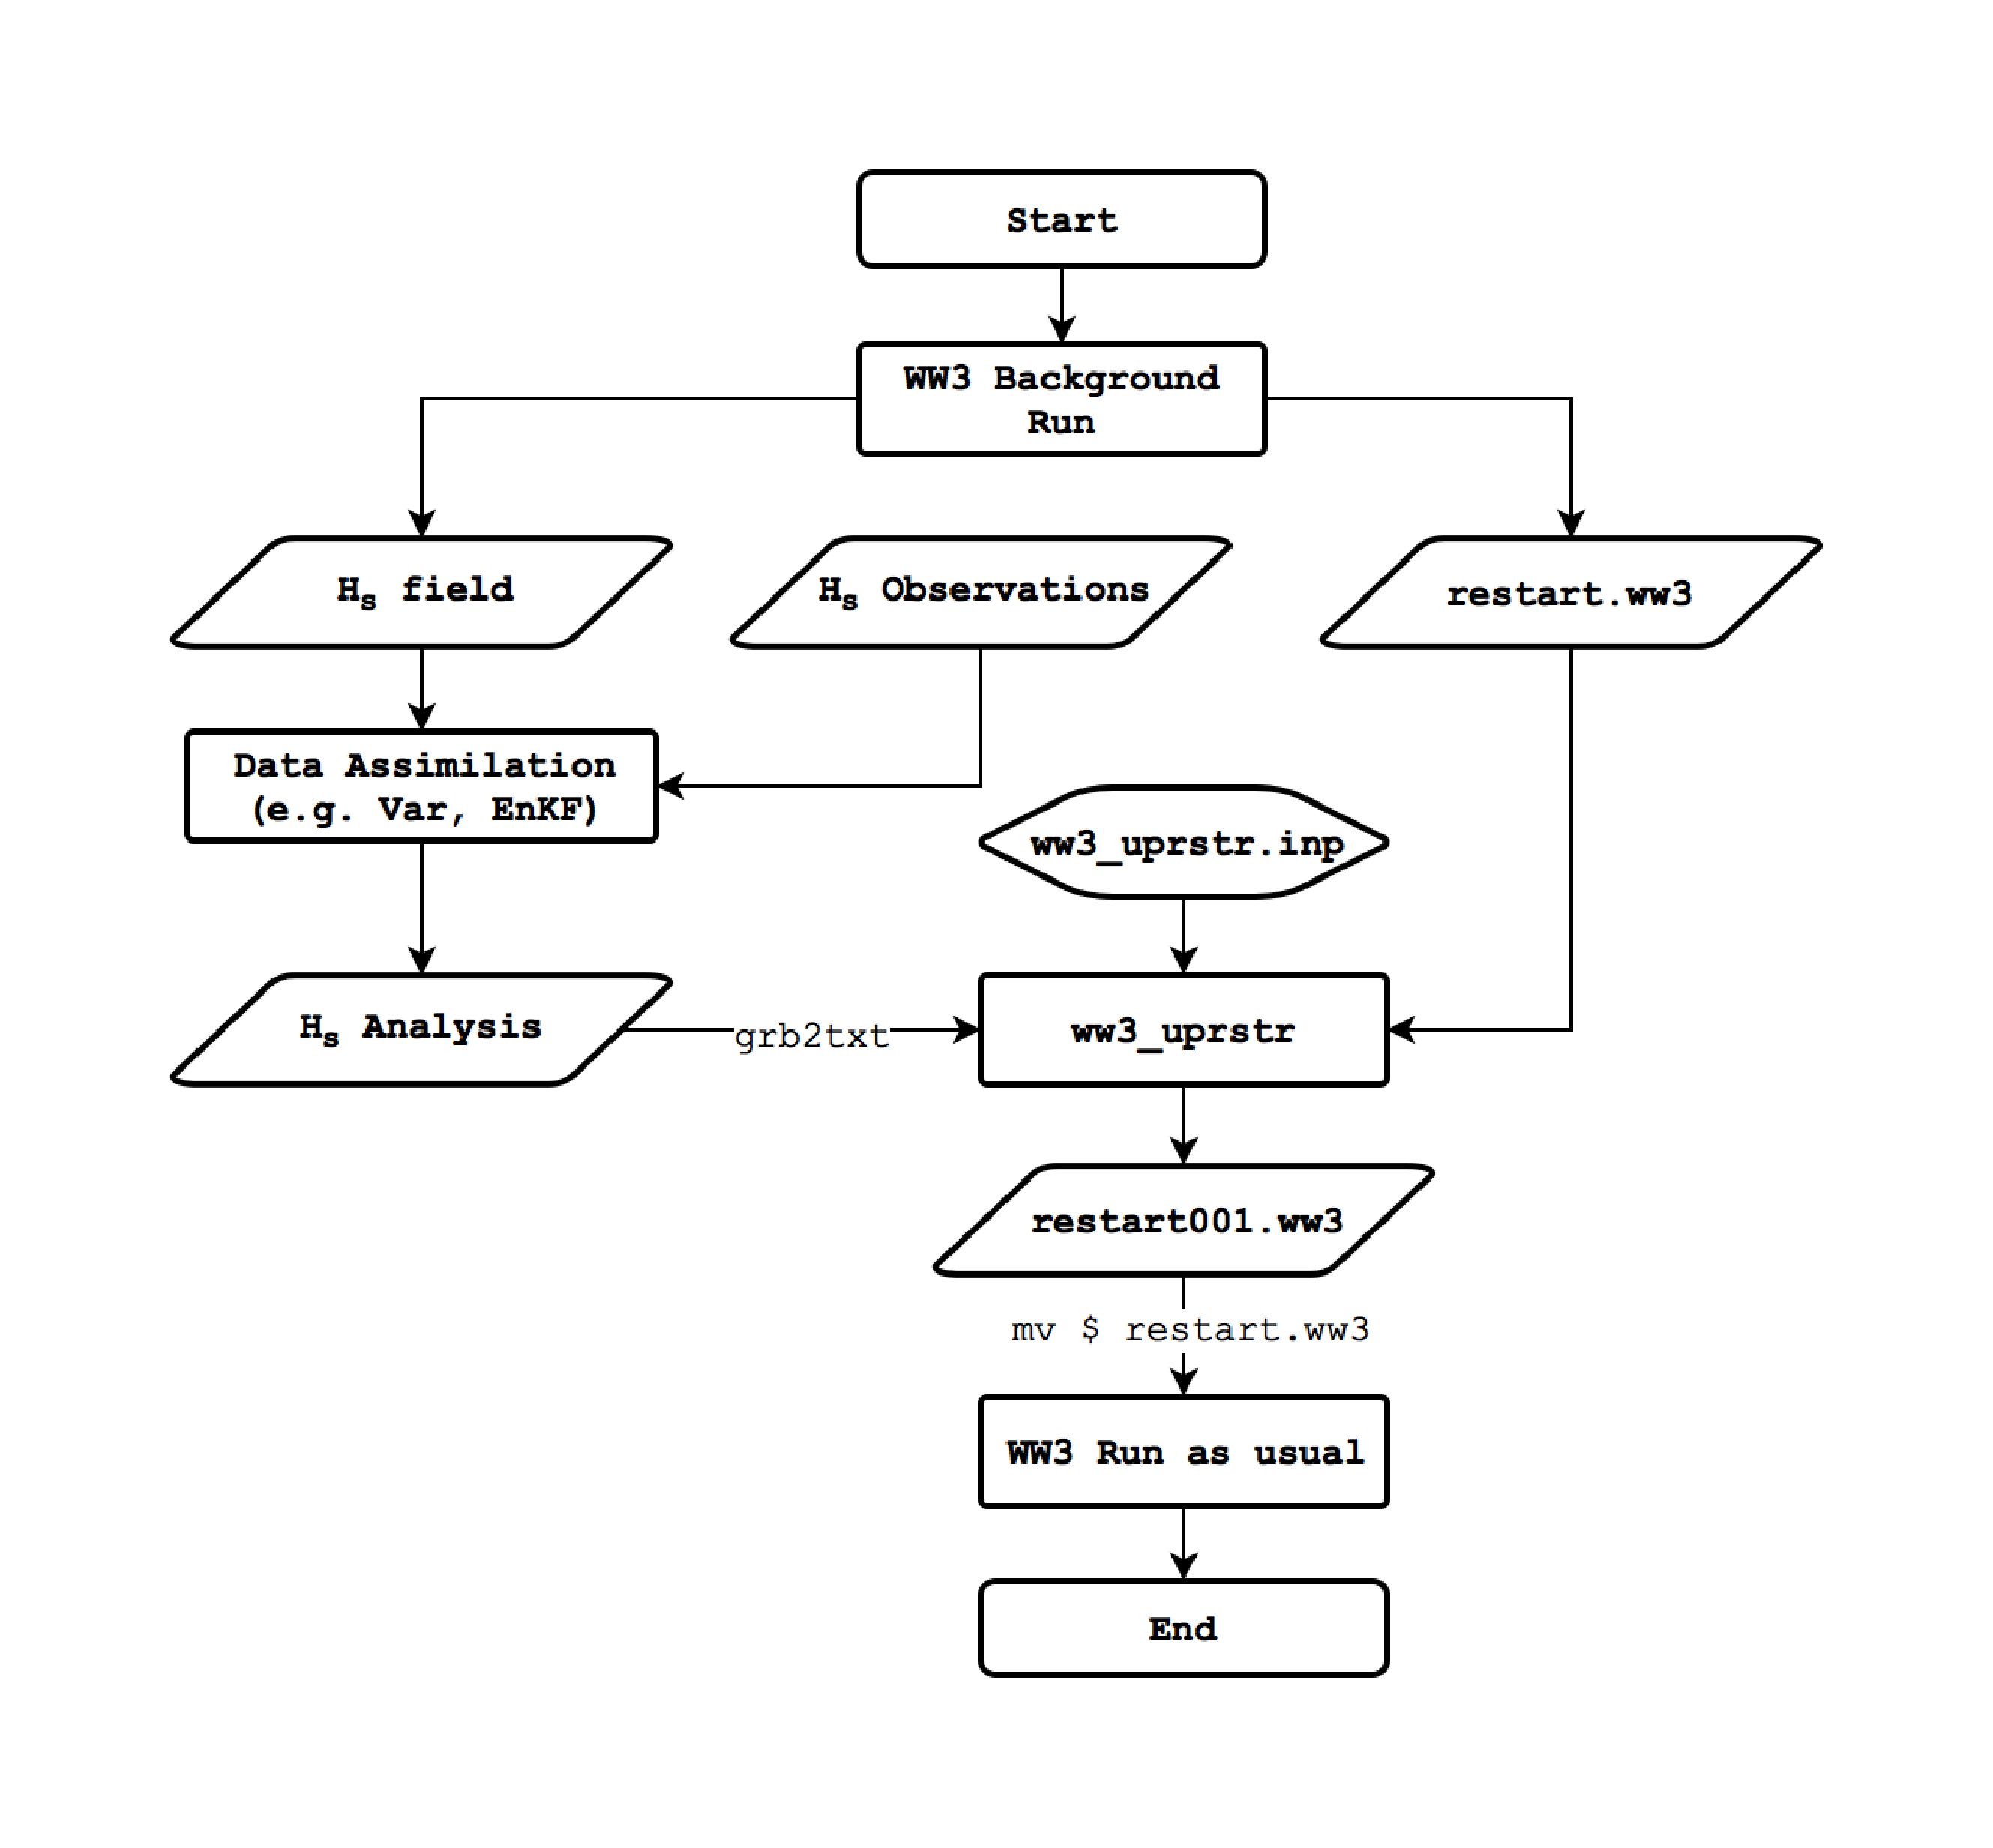
\includegraphics[width=0.9\textwidth]{./run/waveDA.eps}
\caption{简化波浪资料同化系统的流程图，展示 {ww3\_uprstr} 的作用、所需输入文件以及更新后重启动文件的输出结果。}
\label{fig:waveDAflowchart} \botline
\end{center}
\end{figure}

WDA 模块使用背景场和分析时刻可用的观测，生成分析，并以 grbtxt 格式（\textbf{XXXX.grbtxt}）导出 SWH 场。

分析文件、\textbf{mod\_def.ww3}、\textbf{restart.ww3} 文件以及 \textbf{ww3\_uprstr.inp} 是 \textbf{ww3\_uprstr} 的输入文件。如果所有选项和输入文件都准备正确，在单处理器上更新包含 260000 个网格节点的网格并生成输出大约需要一分钟。更新后的重启动文件必须改名为预期文件名；在本例中为 \textbf{restart.ww3}。\newline

   \noindent\fbox{
      \parbox{\textwidth}{
      \textbf{注意：}
      所有 \ncep{} 的 WDA 系统都使用 GRIB2 格式，因此总是需要一个中间步骤将 grib 文件转换为合适格式。所用软件为 WGRIB2，更多信息可从
      \href{http://www.cpc.ncep.noaa.gov/products/wesley/wgrib2}{官方网站} 获取。
      }
   }

%\paragraph{如何更新 ww3\_uprstr \newline}
%添加数据读取器，主要用于机器无关二进制数据和 wgrib2。

\pb


% tab:fields

\begin{table} \begin{center}
\begin{tabular}{|c|c|c|c|c|c|} \hline
组 & 字段 & 说明                  &  文件        & GRIB1 & GRIB2   \\
      &                              &  扩展名   & 数据  & 数据    \\ \hline \hline
 1 & 1 & 水深                           & {\file .dpt} &  --  &    --    \\
 1 & 2 & 平均海流分量         & {\file .cur} &  --  &    --    \\
 1 & 3 & 风速                      & {\file .wnd} &  32  &  0,2,1   \\
   &&  风向                 &              &  31  &  0,2,0   \\
   &&  风 $u$                       &              &  33  &  0,2,2   \\
   &&  风 $v$                       &              &  34  &  0,2,3   \\
 1 & 4 & 气海温差              & {\file .dt}  &  --  &    --    \\
 1 & 5 & 水位                     & {\file .wlv} &  --  &  10,3,1  \\
 1 & 6 & 海冰覆盖率                    & {\file .ice} &  91  &  10,2,0  \\
 2 & 1 & 波高 $H_s$               & {\file .hs}  & 100  &  10,0,3  \\
 2 & 2 & 平均波长                & {\file .l}   &  --  &    --    \\
 2 & 3 & 平均波周期 $T_{m0,2}$     & {\file .t02} &  --  &    --    \\
 2 & 4 & 平均波周期 $T_{m0,1}$     & {\file .t}   & 103  &  10,0,15 \\
 2 & 5 & 平均波周期 $T_{m0,-1}$    & {\file .tm1} &  --  &    --    \\
 2 & 6 & 峰值频率 $f_p$            & {\file .fp}  & 108  &  10,0,11 \\
 2 & 7 & 平均波向 $\theta_m$  & {\file .dir} & 101  &    --    \\
 2 & 8 & 方向扩展 $\sigma$     & {\file .spr} &  --  &    --    \\
 2 & 9 & 峰值方向 $\theta_p$       & {\file .dp}  & 107  &  10,0,10 \\
 4 & 1 & 分区 $H_s$              & {\file .phs} & 102,105 & 10,0,5/8 \\
 4 & 2 & 分区 $T_p$              & {\file .ptp} & 110,106 & 10,0,6/9\\
 4 & 3 & 分区 $L_p$              & {\file .plp} &  --  &    --    \\
 4 & 4 & 分区 $\theta_m$         & {\file .pdir} & 109,104 & 10,0,4/7 \\
 4 & 5 & 分区 $\sigma$           & {\file .psi} &  --  &    --    \\
 4 & 6 & 分区风海比例      & {\file .pws} &  --  &    --    \\
 4 & 7 & 总风海比例         & {\file .wsf} &  --  &    --    \\
 4 & 8 & 分区数            & {\file .pnr} &  --  &    --    \\
 5 & 1 & 摩擦速度分量         & {\file .ust} &  --  &    --    \\
 5 & 2 & 空气侧 Charnock 参数 & {\file .cha} &  --  &    --    \\
 5 & 3 & 能量通量 $\int C_g E(f) df$  & {\file .CgE} &  --  &    --    \\
 5 & 4 & 风到波能量通量        & {\file .faw} &  --  &    --    \\
 5 & 5 & 波支撑应力           & {\file .taw} &  --  &    --    \\
 5 & 6 & 向上波支撑应力    & {\file .twa} &  --  &    --    \\
 5 & 7 & 白冠覆盖率              & {\file .wcc} &  --  &    --    \\
 5 & 8 & 平均白冠泡沫厚度 & {\file .wcf} &  --  &    --    \\
 5 & 9 & 有效破碎波高& {\file .wch} &  --  &    --    \\
 5 & 10 & 白冠矩                 & {\file .wcm} &  --  &    --    \\ \hline
\end{tabular} \end{center}
\caption{~场输出后处理器辅助数据。} \label{tab:fields}
\vspace{0.5in}
\end{table}

\begin{table} \begin{center}
\begin{tabular}{|c|c|c|c|c|c|} \hline
组 & 字段 & 说明                  &  文件        & GRIB1 & GRIB2   \\
      &                              &  扩展名   & 数据  & 数据    \\ \hline \hline
 6 & 1 & 辐射应力                & {\file .Sxy} &  --  &    --    \\
 6 & 2 & 破碎波动量通量     & {\file .two} &  --  &    --    \\
 6 & 3 & Bernoulli 水头                  & {\file .J} &  --  &    --    \\
 6 & 4 & 破碎波能量通量       & {\file .foc} &  --  &    --    \\
 6 & 5 & Stokes 输运                & {\file .tus} &  --  &    --    \\
 6 & 6 & 表层 Stokes 漂移            & {\file .uss} &  --  &    --    \\
 6 & 7 & $k=0$ 处二阶压力  & {\file .p2s} &  --  &    --    \\
 7 & 1 & 近底振幅           & {\file .cfd} &  --  &    --    \\
 7 & 2 & 近底速度            & {\file .ubr} &  --  &    --    \\
 7 & 3 & 床形参数              & {\file .bed} &  --  &    --    \\
 7 & 4 & 到底部边界层的能量通量 & {\file .fbb} &  --  &    --    \\
 7 & 5 & 到底部边界层的动量通量 & {\file .tbb} &  --  &    --    \\
 8 & 1& 平均平方坡度              & {\file .mss} &  --  &    --    \\
 8 & 2 & Phillips 常数               & {\file .msc} &  --  &    --    \\
 9 & 1 & 平均时间步长               & {\file .dtd} &  --  &    --    \\
 9 & 2 & 截止频率 $f_c$         & {\file .fc}  &  --  &    --    \\
 9 & 3 & 截止频率 $f_c$         & {\file .fc}  &  --  &    --    \\
 9 & 4 & X-Y 平流最大 CFL   & {\file .cfx} &  --  &    --    \\
 9 & 5 & $\theta$ 平流最大 CFL & {\file .cfd} &  --  &    --    \\
 9 & 6 & $k$ 平流最大 CFL   & {\file .cfk} &  --  &    --    \\
 10 & 1 & 用户定义 \#1                & {\file .us1} &  --  &    --    \\
 10 & 2 & 用户定义 \#2                & {\file .us2} &  --  &    --    \\ \hline
\end{tabular} \end{center}
\caption*{表~\ref{tab:fields}，续。}
\vspace{0.5in}
\end{table}

\clearpage

\section{~安装、编译和运行波浪模型} \label{chapt:impl}
\newcounters

% 本章正文正按 \input 文件逐节替换为中文；命令、文件名和开关名应在翻译时保持原样。
\vssub
\subsection{~引言}
\vssub

\ws{} 采用 ANSI 标准 \fortran-90 编写，不包含依赖特定机器的元素，因此在大多数平台上都可以不经修改地安装。\ws{} 使用自己的预处理器在编译层面选择模式选项，并打开或关闭测试输出。这种方法在 \ws{} 开发过程中被证明很高效，但也使安装过程更复杂。为尽量减少复杂性，随代码提供了一组 \unix/Linux 脚本，用于自动化一般安装流程，尤其是预处理器的使用。
请注意，该选项不支持 MS 产品等其他操作系统。如果需要在这些平台之一上编译代码，建议先在 \unix/Linux 环境中使用工具 {\code w3\_source}（见下文）提取可工作的代码，然后将这份干净代码移植到目标平台。

\begin{center}
\rule[1mm]{55mm}{1.0mm} 警告 \rule[1mm]{55mm}{1.0mm} \\
\vspace{\baselineskip}
\parbox{120mm}{如果将版本 \WWver{} 作为 \ws{} 旧版本的升级来实现，请注意该版本可能与旧模式版本不兼容。因此，谨慎做法是{\it 不要}把新版 \ws{} 安装在旧版本之上。} \\ \vspace{\baselineskip}
\rule[1mm]{55mm}{1.0mm} 警告 \rule[1mm]{55mm}{1.0mm}
\end{center}

\vssub
\subsection{~发行方式}\label{sec:install}
\vssub

\noindent 到 5.16 版为止，\ws{} 的公开发布版以 tarball 形式发布。6.07 版公开发布之后，\ws{} 将转向开放开发范式，源代码通过 Github 分发。

\vssub
\subsection{~安装}
\vssub

克隆源代码：
\command{ git clone https://github.com/NOAA-EMC/WW3 }
公开发布版可通过检出标签获得：
\command{ git checkout VERTAG }
其中 VERTAG 是公开发布标签，例如 v6.07。

\vssub
\subsection{~设置}
\vssub

克隆 \ws{} 仓库之后，需要执行两个步骤。第一步是运行脚本 {\file model/bin/w3\_setup}；该脚本会编译辅助程序，并设置环境文件 {\file wwatch3.env}，该文件会本地存放在 bin 目录中。此文件设置默认 C 和 FORTRAN 编译器选项，这些选项只由预处理器使用。除特殊情况外，可以直接使用该默认设置。单独运行该脚本会给出完整用法；若要执行设置，还需提供 source\_dir，即 {\file model} 目录的位置。如果从顶层目录运行：
\command{ ./model/bin/w3\_setup model }

可以通过重新运行 {\file w3\_setup} 程序或手工编辑设置文件来修改设置。\ws{} 的 `home' 目录只能通过编辑或删除本地 {\file wwatch3.env} 来更改。

注意，旧版本的 \ws{} 曾要求定义环境位置。一个高级选项是在用户环境变量 {\code WWATCH3\_ENV} 中定义 {\file wwatch3.env} 的路径；现在已不再需要。此外，也不再提供全局安装选项。

设置 \ws{} 的第二步是运行脚本 {\file /model/bin/ww3\_from\_ftp.sh}，以获取未存储在 git 仓库中的二进制文件或大型文件。从顶层目录运行：
\command{./model/bin/ww3\_from\_ftp.sh}
该脚本有三个提示需要用户输入。第一个询问顶层目录路径，第二个询问是否删除复制得到的 tar 文件（通常回答 n，即否），最后一个询问是否保留该脚本使用的文件夹（通常回答 n，即否）。

\vssub
\subsection{~目录结构}
\vssub

克隆 \ws{} 仓库之后，顶层目录中可见以下目录。

\begin{dlist}
\dit{manual   }{手册目录。}
\dit{model    }{模式源代码、构建脚本等。}
\dit{regtests }{\ws{} 可执行程序。}
\dit{guide    }{\ws{} 指南。}
\dit{smc\_docs }{SMC 网格的文档和文件。}
\end{dlist}

\noindent \ws{} 的 `model' 目录中存在以下目录。

\begin{dlist}
\dit{tools }{原始辅助程序（源代码等）。}
\dit{bin }{用于编译和链接的可执行程序与 shell 脚本。}
\dit{ftn }{源代码和 makefile。}
\dit{inp }{输入文件。}
\dit{nml }{Namelist 输入文件。}
\end{dlist}

\noindent 编译代码后，会在 `model' 目录中生成以下目录。

\begin{dlist}
\dit{exe }{\ws{} 可执行程序。}
\dit{mod }{模块文件。}
\dit{obj }{目标文件。}
\end{dlist}

\noindent

{\dir tools} 目录包含各种附加工具，具体内容见实际目录。其中包括贡献的 {\it Matlab} 代码、{\it IDL} 工具、{\it bash} 脚本，以及 {\it GrADS} 和 {\it FORTRAN} 程序。

设置 \ws{} 时，安装流程会首先处理辅助程序的 {\it FORTRAN} 代码，使用设置文件 {\file wwatch3.env} 中定义的编译器。注意，这些代码仍采用固定格式的 {\fortran-77}。可执行程序存储在 {\dir bin} 目录中。关于这些程序的更详细说明（包括运行可执行程序的说明），可在上述源代码文件包含的文档中找到。编译这些程序后，若干 \unix{} shell 脚本和辅助文件会安装到 {\dir bin} 目录中。

\begin{flist}
\fit{w3adc.f }{\ws{} 的 {\fortran} 预处理器。}
\fit{w3prnt.f}{打印文件（源代码），包括页码和行号。}
\fit{w3list.f}{生成通用源代码清单。}

\fit{w3split.f}{从点输出后处理器的谱输出中生成谱公告，用以识别一个谱内的各个波浪场（见 \para\ref{sec:ww3outp}）。这是一段旧代码，已被直接从 {\file ww3\_outp} 生成公告的方式取代。这里保留它仅出于历史原因。}

\end{flist}

{\dir bin} 目录包含用于管理 \ws{} 框架的各种 \unix{} 脚本。这些脚本的用法在 \para\ref{sec:comp} 中说明。注意，以下脚本会从 \ws{} 环境设置文件获取设置信息，该文件由 {\code WWATCH3\_ENV} 定义；它既可以由读取本地 {\file wwatch3.env} 的 {\file w3\_setenv} 定义，也可以由用户环境文件定义。

\vspace{\baselineskip} \noindent
使用的主程序：

\begin{flist}
\fit{install\_ww3\_tar }{从 tar 文件安装 \ws{} 的脚本。}
\fit{w3\_setup        }{创建/编辑 \ws{} 环境设置文件的脚本。默认设置文件为 {\file {\dir bin}/.wwatch3.env}。switch 和编译器通过参数给出（见选项）。}
\fit{w3\_clean        }{清理 \ws{} 目录的脚本，通过删除编译或测试运行生成的文件完成清理。提供 3 个清理级别（见选项）。}
\fit{w3\_make         }{使用 makefile 编译并链接 \ws{} 组件的脚本。可在参数中给出程序列表。}
\fit{w3\_automake      }{根据 switch 文件内容，在 MPI、OMP 或 HYB 中分别自动编译串行程序和分布式程序的脚本。可在参数中给出程序列表。}
\fit{w3\_new          }{在结合 makefile 使用时，触碰所有正确的源代码文件，以处理编译器开关变化的脚本。}
\fit{ww3\_gspl.sh     }{自动使用 {\file ww3\_gspl} 程序的脚本（见 \para\ref{sub:ww3gspl}）。}
\fit{arc\_wwatch3\_tar}{将 \ws{} 的版本归档到目录 {\dir arc} 中的程序。}
\fit{ww3\_from\_ftp.sh  }{下载 git 未提供的所有二进制文件的脚本。}
\end{flist}

\noindent
提供的示例文件：

\begin{flist}
\fit{switch\_{\it xxx} }{用户或开发者提供的预处理器开关示例（\para\ref{sec:switches}）。}
\end{flist}

\noindent
被调用的子程序：

\begin{flist}
\fit{w3\_setenv        }{基于 {\file {\dir bin}/.wwatch3.env} 设置环境的脚本。由所有辅助程序调用。}
\fit{comp.tmpl        }{与 {\file cmplr.env} 配合使用的编译脚本模板 {\file comp}。}
\fit{link.tmpl        }{与 {\file cmplr.env} 配合使用的链接脚本模板 {\file link}。}
\fit{cmplr.env        }{在 intel、mpt、gnu、pgi 上测试过的编译器选项，包含优化和调试选项；与 comp.tmpl 和 link.tmpl 配合使用。}
\fit{make\_makefile.sh}{根据文件 {\file switch} 中的选择生成 makefile 的脚本。}
\fit{ad3              }{对给定源代码文件运行预处理器 {\file w3adc} 和编译脚本 {\file comp} 的脚本。}
\fit{ad3\_test        }{{\file ad3} 的测试版本，显示对原始源文件的修改。该脚本不编译代码。}
\fit{all\_switches    }{生成源代码文件中存在的所有 {\code w3adc} 开关列表。}
\fit{find\_switch     }{查找包含编译器开关（或任意字符串）的 \ws{} 源代码文件的脚本。}
\fit{sort\_switch     }{对 switch 文件中的开关排序。}
\fit{sort\_all\_switches}{搜索 \ws{} 中所有 switch 文件并调用 {\file sort\_switch} 的脚本。}

\end{flist}


\noindent
额外程序：

\begin{flist}
\fit{comp.{\it xxx}   }{用于高级设置的编译脚本 {\file comp}。}
\fit{link.{\it xxx}   }{用于高级设置的链接脚本 {\file link}。}
\fit{make\_MPI        }{分别编译 MPI 和非 MPI 程序的脚本（未来版本中废弃，请使用 {\file w3\_automake}）。}
\fit{make\_OMP        }{分别编译 OpenMP 和单线程程序的脚本（未来版本中废弃，请使用 {\file w3\_automake}）。}
\fit{make\_HYB        }{分别编译混合 MPI-OpenMP 程序和单线程程序的脚本（未来版本中废弃，请使用 {\file w3\_automake}）。}
\fit{ln3              }{将源代码文件符号链接到工作目录的脚本（未使用）。}
\fit{list             }{使用 {\file w3prnt} 打印源代码清单的脚本（未使用）。}
\fit{w3\_source       }{为任意 \ws{} 程序元素生成真正 \fortran{} 源代码的脚本（未使用）。}
\fit{WW3\_switch\_process}{从源文件处理 switch 的 Perl 脚本（未使用）。}
\end{flist}


安装到 {\dir bin} 目录后，若干 GrADS 脚本会安装到 {\dir tools} 目录中。

\begin{flist}
\fit{cbarn.gs         }{用于显示色标的半标准 GrADS 脚本。}
\fit{colorset.gs      }{定义阴影所用颜色的脚本。}
\fit{profile.gs}      {显示 {\file ww3\_multi} 生成的剖析数据的脚本。}
\fit{source.gs}       {用于谱和源项组合绘图的脚本（二维极坐标或笛卡尔图，可为彩色或黑白）。}
\fit{1source.gs}      {绘制单个源项的脚本。}
\fit{spec.gs}         {绘制谱的脚本。}
\fit{spec\_ids.gen}   {谱/源项脚本使用的数据文件。}
\end{flist}



\pb

\pb
\vssub
\subsection{~可选环境设置}
\vssub

编译启用 NetCDF 的 \ws{} 程序需要 NetCDF 4.1.1 或更高版本。还需要设置以下环境变量：
\begin{clist}
\cit {NETCDF\_CONFIG} {NetCDF-4 nc-config 工具程序的路径。}
\end{clist}
{\file nc-config} 工具程序用于确定编译所需的合适编译和链接标志。
使用命令
\command{\code nc-config --version} 检查已安装 Fortran-NetCDF 库的版本。同时还要求 NetCDF-4 安装在编译时启用 NetCDF-4 API。使用 \command{\code nc-config --has-nc4} 检查已安装的 NetCDF 是否启用了 NetCDF-4 API。

\vspace{\baselineskip}
\noindent
若要在（三角形非结构网格的显式/隐式）区域分解选项中使用 PDLIB 编译 WAVEWATCH III，需要将环境变量 {\code METIS\_PATH} 设置为 {\code Metis} 和 {\code ParMetis} 的编译路径；它们应使用与 WW3 相同的编译器编译。

\vspace{\baselineskip}
\noindent
关于模式并行版本（OpenMP 和 \mpi{} 版本）还需说明两点。首先，在准备可于 \mpi{} 环境中运行的可执行程序时可能会出现复杂情况。这些复杂情况在附录~\ref{app:mpi} 中讨论。其次，\omp{} 代码应只使用指令方式编译，也就是说，不要使用会自动对代码进行线程化的编译器选项。



\vssub
\subsection{~编译和链接} \label{sec:comp}
\vssub

\vspace{\baselineskip} \noindent
首次编译前，必须使用脚本 {\file w3\_setup} 设置 \ws{} 环境，并把模式目录路径作为参数传入。该脚本提供若干选项，用于定义编译器选项以及位于 {\dir bin} 目录中的 switch 文件。例如，\command{w3\_setup /home/user/WW3/model -c <comp> -s <switch>} 中，{\code <comp>} 关键字可以是 {\code mpt}、{\code intel}、{\code gfortran}、{\code pgi}，表示优化编译选项；也可以是 {\code mpt\_debug}、{\code intel\_debug}、{\code gfortran\_debug}、{\code pgi\_debug}，表示调试编译选项。如果需要依赖系统的选项，可通过修改脚本 {\file cmplr.env} 完成。不同集群的一些旧 comp/link 模板仍然可用，但不推荐使用。{\code <switch>} 关键字可以是已提供 switch 文件的后缀，也可以是你自己的后缀。运行该脚本会创建以下三个脚本/文件：

\begin{flist}
\fit{comp}  {编译器脚本。该脚本基于 {\file comp.tmpl}，并使用给定的编译器及其选项定义。}
\fit{link}  {链接器脚本。该脚本基于 {\file link.tmpl}，并使用给定的链接器及其选项定义。}
\fit{switch}{包含预处理器 {\file w3adc} 可识别开关列表的文件。从 {\code switch\_<switch>} 复制而来。}
\end{flist}

\vspace{\baselineskip}

环境文件 {\file wwatch3.env} 会被创建；如果它已经存在，则会被更新。用于代码预处理器的辅助 FORTRAN 程序默认会使用 GNU FORTRAN 编译器编译，该编译器可能不同于为 \ws{} 程序提供的编译器。


\vspace{\baselineskip} \noindent
编译 \ws{} 最简单的方法是使用脚本 {\file w3\_automake}，由它自动检测要编译哪些程序并完成编译。它会强制将前处理和后处理程序编译为串行实现，而其他程序则依据 OpenMP、MPI 或混合配置中的开关决定。如果 netCDF 库设置正确，专用于 netCDF 的程序也会被编译。对 SCRIPNC、PDLIB、OASIS、ESMF、TRKNC 和 TIDE 关键字也会进行同样测试，以便以最佳方式管理程序编译。例如，\command{w3\_automake}，或只编译少数程序时使用 \command{w3\_automake ww3\_grid ww3\_shel ww3\_ounf}；编译后的程序都会存放在 {\dir exe} 目录中，并附带所用 switch、comp 和 link 文件的副本。

\vspace{\baselineskip} \noindent
如果程序编译出现问题，日志文件会存放在临时目录中；串行模式使用 {\dir tmp\_SEQ}，MPI 等分布式模式使用 {\dir tmp\_MPI}，OMP 使用 {\dir tmp\_OMP}，混合模式使用 {\dir tmp\_HYB}。每个程序通常有三个日志文件：

\begin{flist}
\fit{\code ww3\_<prog>.l} {完整程序，只保留基于开关匹配到的代码行，并在末尾包含编译命令行。}
\fit{\code ww3\_<prog>.out} {警告消息。}
\fit{\code ww3\_<prog>.err} {错误消息。}
\end{flist}

若要从 \ws{} 框架中移除所有用户创建的文件，可以使用脚本 {\file w3\_clean}；仅清理 {\dir model} 目录时使用 \command{w3\_clean -m}，清理完整 ww3 仓库时使用 \command{w3\_clean -c}。


\vssub
\subsection{~详细编译}
\vssub

\ws{} 的编译通过 {\dir bin} 目录中的脚本 {\file w3\_make} 完成\footnote{~注意，在运行 {\file w3\_make} 之前，需要按本节余下部分的说明进行若干用户干预。}。如果不带参数使用该脚本，将编译 \ws{} 的所有基本程序。也可以在编译命令中给出要编译的程序名。例如，\command{w3\_make ww3\_grid ww3\_strt} 只会编译网格预处理器和初始条件程序。{\file w3\_make} 使用上一节介绍的多个脚本。图~\ref{fig:make} 给出了图示说明。如有必要，脚本 {\file w3\_make} 会使用脚本 {\file make\_makefile.sh} 生成 makefile。{\file make\_makefile.sh} 根据文件 {\file switch} 中的程序开关（见 \para\ref{sec:switches}）生成要链接的模块列表，并检查所有所需源文件的模块依赖。如果自上次调用 {\file w3\_make} 以来开关发生了变化，{\file w3\_new} 会用于 `touch' 相关源代码，或删除相关目标文件。makefile 完成后，标准 \unix{} make 工具用于编译和链接程序。makefile 不直接调用 \fortran{} 编译器，而是调用预处理器和编译脚本 {\file ad3} 与 {\file comp}，以及链接脚本 {\file link}。脚本 {\file ad3} 使用文件名扩展名判断需要执行的操作。扩展名为 {\file .ftn} 的文件由 {\code w3adc} 处理；扩展名为 {\file .f} 或 {\file .f90} 的文件则直接发送到脚本 {\code comp}。尽管用户可以交互式尝试其中若干脚本，通常只需要运行 {\file w3\_make}。

\input{zh/impl/fig_make_zh}

\vspace{\baselineskip}

\begin{center}
\rule[1mm]{55mm}{1.0mm} 警告 \rule[1mm]{55mm}{1.0mm} \\
\vspace{\baselineskip}
\parbox{120mm}{辅助脚本 {\file w3\_make} 等使用的是 \ws{} 主目录下 {\file ./bin} 目录中的 {\file switch}、{\file comp} 和 {\file link} 文件，{\it 不是}本地目录中的文件。} \\ \vspace{\baselineskip} \rule[1mm]{55mm}{1.0mm} 警告
  \rule[1mm]{55mm}{1.0mm}
\end{center}


\noindent
完成适当修改或复制入适当示例脚本之后，即可编译并链接 \ws{} 的（部分）程序。首次编译程序时，建议逐个编译程序组成部分，以避免冗长的错误消息，并在 {\file comp} 中设置错误捕获。一个好的起点是编译简单测试代码 {\F ctest}。首先进入目录 {\dir work}，并通过输入 \command{ln3 ctest} 创建到该例程源代码的链接。创建该链接是为了便于稍后加入错误，以测试或设置脚本 {\file comp} 中的错误捕获。输入命令 \command{ad3\_test ctest} 可以查看预处理器 {\file w3adc} 的内部工作方式；该命令会显示实际源代码如何由 {\file ctest.ftn}、包含文件和程序开关构造而成。接下来，可通过输入 \command{ad3 ctest 1} 测试该子程序的编译；它会同时调用预处理器 {\file w3adc} 和编译脚本 {\file comp}。该行末尾的 1 会激活测试输出。如果省略它，该命令应只产生一行输出，用于标识正在处理的例程。如果 {\file ad3} 按预期工作，会生成目标文件 {\file obj/ctest.o}。如果初始设置时提出了请求，则可在暂存目录中找到源代码和清单文件（{\file ctest.f} 与 {\file ctest.l}）。如果 {\file comp} 检测到编译错误，也会保留清单文件。此时，谨慎做法是在 work 目录中的 {\file ctest.ftn} 中加入错误和警告，测试脚本 {\file comp} 的错误捕获。错误捕获在 {\file comp} 文档中有较详细讨论。测试 {\file comp} 并移除 {\file ctest.ftn} 中的错误之后，可以删除到 work 目录的链接以及文件 {\file obj/ctest.o}。

单个例程成功编译后，下一步是尝试编译并链接一个完整程序。可以输入 \command{w3\_make ww3\_grid} 来编译网格预处理器。如果编译看起来成功，并且输入文件已经安装（见上文），可以在 work 目录中输入 \command{ww3\_grid} 测试网格预处理器。如果输入文件已经安装，work 目录中会存在指向输入文件 {\file ww3\_grid.inp} 的链接，网格预处理器会运行并把输出发送到屏幕。网格预处理器的输出文件会出现在 work 目录中。首次编译某个程序时，操作系统可能找不到可执行程序。如果发生这种情况，尝试输入 \command{rehash}，或打开一个新的 shell 继续工作。通过这种方式，所有单独程序都可以被编译和测试。若要清理所有临时文件（如清单）以及测试运行的数据文件，输入 \command{w3\_clean}。注意，{\file w3\_make} 只检查 switch 文件是否发生变化。如果用户修改了编译和链接脚本 {\file comp} 与 {\file link} 中的编译选项，建议强制重新编译整个程序。可以在调用 {\file w3\_make} 之前输入 \command{w3\_new all {\rm or} w3\_new} 来实现。如果编译无明显原因地失败，这样做也可能有用。


\vssub
\subsection{~选择模式选项} \label{sec:switches}
\vssub

{\file bin} 目录中的文件 {\file switch} 包含一组字符串，用于标识要选择的模式选项。可用选项很多。其中若干组选项要求必须且只能选择一个。这些强制开关在 \para\ref{sub:man_switch} 中说明。其他开关是可选的，在 \para\ref{sub:opt_switch} 中说明。默认模式设置在 \para\ref{sub:opt_default} 中说明。开关在 {\file switch} 中出现的顺序是任意的。这些开关如何包含到源代码文件中，见 \para\ref{sec:w3adc}。

\vsssub
\subsubsection{~强制开关} \label{sub:man_switch}
\vsssub

以下每组开关都必须且只能选择一个。硬件模式（第一组）和消息传递协议（第二组）如下。注意，这两组共享一个开关。这意味着 {\sc mpi} 开关只能与 {\sc dist} 开关组合使用。
\begin{slist}
\sit{shrd}{共享内存模式。}
\sit{dist}{分布式内存模式。}
\end{slist}

\begin{slist}
\sit{shrd}{共享内存模式，无消息传递。}
\sit{mpi} {消息传递接口（MPI）。}
\end{slist}

\noindent
传播格式和 GSE 缓解方法的选择。它们表示两组开关，两组之间有一些共享开关。注意，第二组开关从属于第一组开关中的程序模块选择，因此没有用户定义选项。
\begin{slist}
\sit{pr0} {不使用传播格式 / GSE 缓解。}
\sit{pr1} {一阶传播格式，无 GSE 缓解。}
\sit{pr2} {带 \cite{art:BH87} 色散修正的高阶格式。}
\sit{pr3} {带 \cite{tol:OMOD02b} 平均技术的高阶格式。}
%\sit{pr4} {带 \cite{tol:OMOD02b}
%           散度技术的 \uq\ 传播格式。}
\end{slist}

\begin{slist}
\sit{pr0} {不使用传播格式。}
\sit{pr1} {一阶传播格式。}
\sit{uno} {二阶（UNO）传播格式。}
\sit{uq } {三阶（UQ）传播格式。}
\end{slist}

\noindent
通量计算的选择：
\begin{slist}
\sit{flx0} {不使用例程；通量计算包含在源项中。}
\sit{flx1} {根据式~(\ref{eq:Wu}) 计算摩擦速度。}
\sit{flx2} {来自 Tolman and Chalikov 输入的摩擦速度。}
\sit{flx3} {同上，但带式~(\ref{eq:Cd_cap_1}) 或 (\ref{eq:Cd_cap_2}) 的上限。}
\sit{flx4} {根据式~(\ref{eq:ST607}) 计算摩擦速度。}
\sit{flx5} {来自大气应力的摩擦速度（应力应作为输入）。}
\end{slist}

\noindent
线性输入的选择：
\begin{slist}
\sit{ln0} {无线性输入。}
\sit{seed}{式~(\ref{eq:seed}) 的谱播种。}
\sit{ln1} {带滤波器的 Cavaleri and Malanotte-Rizzoli。}
\end{slist}

\noindent
输入与耗散的选择。{\F stab{}\it n} 开关是可选的，并且是对应 {\F st{\it n}} 开关的附加项：
\begin{slist}
\sit{st0} {不使用输入与耗散。}
\sit{st1} {\wam\-3 源项包。}
\sit{st2} {\cite{tol:JPO96} 源项包。另见可选开关 {\F stab2}。}
\sit{stab0}{无稳定度修正。与任何源项（{\F st}）包兼容。包含该开关没有效果。}
\sit{stab2}{启用稳定度修正 (\ref{eq:scor})--(\ref{eq:stab})。仅与 {\F st2} 兼容。}
\sit{st3} {\wam\-4 及其变体源项包。}
\sit{stab3}{启用来自 \cite{rep:AB02} 的稳定度修正。仅与 {\F st3} 和 {\F st4} 兼容。}
\sit{st4} {\cite{art:Aea10} 源项包。}
%\sit{st5} {UNSW 源项包。}
\sit{st6} {BYDRZ 源项包。}
\end{slist}

\noindent
非线性相互作用的选择：
\begin{slist}
\sit{nl0} {不使用非线性相互作用。}
\sit{nl1} {离散相互作用近似（\dia）或 Gaussian Quadrature Method（GQM）。}
\sit{nl2} {精确相互作用近似（\xnl）。}
\sit{nl3} {广义多重 \dia{}（\gmd{}）。}
\sit{nl4} {双尺度近似（TSA）。}
\end{slist}

\noindent
底摩擦的选择：
\begin{slist}
\sit{bt0} {不使用底摩擦。}
\sit{bt1} {\js\ 底摩擦公式。}
%\sit{bt2} {??? 底摩擦公式。}
%\sit{bt3} {??? 底摩擦公式。}
\sit{bt4} {\showex\ 底摩擦公式。}
\sit{bt8} {Dalrymple and Liu 公式（流体泥海底）。}
\sit{bt9} {Ng 公式（流体泥海底）。}
\end{slist}

\noindent
海冰阻尼项的选择：
\begin{slist}
\sit{ic0} {无海冰阻尼。}
\sit{ic1} {简单公式。}
\sit{ic2} {Liu et al. 公式。}
\sit{ic3} {Wang and Shen 公式。}
\sit{ic4} {随频率变化的海冰阻尼。}
\end{slist}

\noindent
海冰散射项的选择：
\begin{slist}
\sit{is0} {无海冰散射。}
\sit{is1} {海冰扩散散射（简单）。}
\sit{is2} {依赖浮冰尺寸的散射和耗散。}
\end{slist}

\noindent
反射项的选择：
\begin{slist}
\sit{ref0} {无反射。}
\sit{ref1} {启用海岸线和冰山反射。}
\end{slist}

\noindent
水深诱导破碎的选择：
\begin{slist}
\sit{db0} {不使用水深诱导破碎。}
\sit{db1} {Battjes-Janssen。}
\end{slist}

\noindent
三波相互作用的选择：
\begin{slist}
\sit{tr0} {不使用三波相互作用。}
\sit{tr1} {集总三波相互作用（LTA）方法。}
\end{slist}

\noindent
底部散射的选择：
\begin{slist}
\sit{bs0} {不使用底部散射。}
\sit{bs1} {Magne and Ardhuin。}
\end{slist}

\noindent
风/动量/空气密度插值方法（时间）的选择：
\begin{slist}
\sit{wnt0}{无插值。}
\sit{wnt1}{线性插值。}
\sit{wnt2}{近似二次插值。}
\end{slist}

\noindent
风/动量插值方法（空间）的选择：
\begin{slist}
\sit{wnx0}{矢量插值。}
\sit{wnx1}{近似线性速度插值。}
\sit{wnx2}{近似二次速度插值。}
\end{slist}

\noindent
流插值方法（时间）的选择：
\begin{slist}
\sit{crt0}{无插值。}
\sit{crt1}{线性插值。}
\sit{crt2}{近似二次插值。}
\end{slist}

\noindent
流插值方法（空间）的选择：
\begin{slist}
\sit{crx0}{矢量插值。}
\sit{crx1}{近似线性速度插值。}
\sit{crx2}{近似二次速度插值。}
\end{slist}

\noindent
用户提供 GRIB 包的开关。
\begin{slist}
\sit{nogrb}{不包含包。}
\sit{ncep2}{用于 IBM SP 的 \ncep\ GRIB2 包。}
\end{slist}

% -------------------------------------------------------------
\vsssub
\subsubsection{~可选开关} \label{sub:opt_switch}
\vsssub

以下所有开关在被选择时都会激活模式行为，但不要求特定组合。以下开关控制 \ws{} 程序的可选输出。

\begin{slist}
\sit{o0}  {网格预处理器中 namelist 的输出。}
\sit{o1}  {网格预处理器中边界点的输出。}
\sit{o2}  {网格预处理器中网格点状态图的输出。}
\sita{o2} {网格预处理器中生成陆海掩膜文件 {\file mask.ww3}。}
\sitb{o2} {网格预处理器中障碍物图的输出。}
\sitc{o2} {以 {\file ww3\_grid} 读取的格式打印状态图。}
\sit{o3}  {场预处理器中场循环的附加输出。}
\sit{o4}  {初始条件程序中归一化一维能量谱的打印图。}
\sit{o5}  {同上，二维能量谱。}
\sit{o6}  {同上，波高的空间分布（未适配分布式内存）。}
\sit{o7}  {通用壳中均匀场输入数据的回显。}
\sita{o7} {输出点的诊断输出。}
\sitb{o7} {同上，在 {\file ww3\_multi} 中。}
\sit{o8}  {在波浪模式中筛除极小波高的场输出（对某些传播测试有用）。}
\sit{o9}  {在波浪模式中将负能量指定为负波高。用于新传播格式的测试阶段。}
\sit{o10} {在标准输出中标识多网格模式扩展的主要元素。}
\sit{o11} {{\file log.mww3} 中管理算法的附加日志输出。}
\sit{o12} {标识重叠网格中被移除的边界点（中心）。}
\sit{o13} {标识重叠网格中被移除的边界点（边缘）。}
\sit{o14} {为 {\file ww3\_outp} 中输出类型 {\code ITYPE = 0} 生成带浮标数据的日志文件 {\file buoy\_log.ww3}。}
\sit{o15} {在 {\file ww3\_prep} 中生成带输入数据文件时间戳的日志文件 {\file times.XXX}。}
\sit{o16} {在 {\file ww3\_gspl} 中生成网格分区的 GrADS 输出。}
\end{slist}

\noindent
以下开关使用 \omp{} 指令启用模式并行化，也称为 `threading'。在模式 5.01 版之前，线程化与使用 {\sc mpi} 开关的并行化不能同时使用。从 5.01 版开始，可以使用纯 MPI、纯 OMP 和混合 MPI-OMP 方法。5.01 版及更高版本使用的开关与旧模式版本中使用的开关不兼容。
\begin{slist}
\sit{ompg}{通用循环并行化指令，同时用于纯 OpenMP 并行化和混合 MPI-OpenMP 并行化。}
\sit{omph}{同上，但仅用于混合 MPI-OpenMP 并行化的指令。}
\sit{pdlib}{三角形非结构网格上显式和隐式求解器的区域分解（该选项需要 {\code ParMetis}）。}
\sit{b4b}{强制启用 OpenMP 的代码实现逐位可复现。某些 OpenMP 操作（尤其是求和等归约）可能由于浮点舍入误差，在不同运行之间产生略有不同的结果。该开关启用中间步骤（例如将数值缩放为整数值），以确保不同运行之间的结果逐位可复现。适用于运行需要这种可复现性的回归测试。目前只影响使用 {\F smc} 开关编译的代码。}
\end{slist}
注意，这些开关只能以特定组合使用，模式安装脚本（特别是 {\file make\_makefile.sh}）会强制执行这一点。纯 MPI 方法需要 {\F dist} 和 {\F mpi} 开关。纯 OpenMP 方法需要 {\F shrd} 和 {\F ompg} 开关，混合方法需要 {\F dist}、{\F mpi}、{\F ompg} 和 {\F omph} 开关。

\vspace{\baselineskip}
\noindent
以下开关与连续移动网格选项有关。第一个开关激活该选项，另外两个是可选附加项。
\begin{slist}
\sit{mgp }{激活式~(\ref{eq:bal_move}) 中的传播修正。}
\sit{mgw }{在移动网格方法中应用风修正。}
\sit{mgg }{激活式~(\ref{eq:move_GSE_avg2}) 中的 GSE 缓解修正。}
\end{slist}

\noindent
此外，还提供以下杂项开关：
\begin{slist}
\sit{cou} {激活耦合所需变量的计算。}
\sit{dss0}{关闭扩散色散修正中的频率色散。}
\sit{fld1}{依赖海况的 $\tau$，\citet{art:Rei14}（\para\ref{sec:FLD1}）。}
\sit{fld2}{依赖海况的 $\tau$，\citet{art:Don12}（\para\ref{sec:FLD2}）。}
\sit{ig1} {二阶谱和自由次重力波（\para\ref{sec:IG1}）。}
\sit{mlim}{使用式~(\ref{eq:MLIM}) 的 Miche 型浅水限制器。}
\sit{mpibdi}{多网格模式初始化的实验性并行化。}
\sit{mpit}{\mpi{} 初始化的测试输出。}
\sit{mprf}{在 {\file ww3\_multi} 中对单个模式和嵌套进行剖析。}
\sit{nco} {面向 NCO（NCEP Central Operations）业务实现的代码修改。主要改变单元号和文件名。不建议一般使用。}
\sit{nls }{激活非线性平滑器（\para\ref{sec:NLS}）。}
\sit{nnt} {生成文件 test\_data\_{\it{nnn}}.ww3，其中包含用于 NNIA 训练和测试的谱与非线性相互作用。}
\sit{oasis }{初始化 OASIS 耦合器（App.~\ref{sec:couplingB}）。}
\sit{oasacm}{OASIS 大气模式耦合场（App.~\ref{sec:couplingB}）。}
\sit{oasocm}{OASIS 海洋模式耦合场（App.~\ref{sec:couplingB}）。}
\sit{oasicm}{OASIS 海冰模式耦合场（App.~\ref{sec:couplingB}）。}
\sit{refrx} {启用基于相速空间梯度的折射（\para\ref{sec:ICE3}）。}
\sit{reft}{海岸线反射的测试输出（由 {\F ref1} 激活）。}
\sit{rtd} {旋转网格选项。}
\sit{rwnd}{按流速修正风速。}
\sit{s}   {通过激活对子程序 {\F strace} 的调用，在主要 \ws{} 子程序中启用子程序跟踪。}
\sit{scrip   }{启用 SCRIP 重映射例程（App. \ref{sec:scripC}）。}
\sit{scripnc }{启用将重映射权重存储在 NetCDF 文件中（App. \ref{sec:scripC}）。}
\sit{sec1}{启用小于 1~s 的全局时间步长，但不允许以小于 1~s 的时间步输出。}
\sit{smc} {激活 SMC 网格。}
\sit{t}   {在整个程序中启用测试输出。}
\sitn{t}  {同上。}
\sit{tdyn}{扩散色散修正中涌浪年龄的动态增量（仅测试案例）。}
\sit{tide }{启用潮汐分析：用于输入文件预处理、ww3\_shel 中的运行时潮汐预报，或使用 ww3\_prtide 进行潮汐预报。}
\sit{tidet}{潮汐分析的测试输出。}
\sit{trknc} {激活波浪系统跟踪后处理程序中的 NetCDF API。}
\sit{uost}{启用未解析障碍物源项。}
\sit{wrst}{在重启动中保存风，并在 wmesmf 的第一个时间步中使用。}
\sit{xw0 }{\uq\ 格式中仅涌浪扩散。}
\sit{xw1 }{同上，仅波浪增长扩散。}
\end{slist}

\vsssub
\subsubsection{~默认模式设置} \label{sub:opt_default}
\vsssub

直到模式 3.14 版，NCEP 业务模式设置都被视为默认模式设置。然而，随着 \ws{} 后续版本的发展，该模式已经演化为一个建模框架，而不是单一模式。因此，各中心以不同方式运行 \ws{}，也就不再能明确识别一个“默认”的模式版本。尽管如此，为了能够在出版物中简洁地精确标识所使用的模式设置，目前在 {\file bin} 目录中提供了各中心的“默认”配置。这些配置以示例 switch 文件和 README 文件的形式提供，例如 {\file switch\_NCEP\_st2} 和 {\file README.NCEP}。注意，这些文件用于简化对模式版本的引用，但并不意味着认可特定的模式配置；在此语境下还应注意，业务中心的模式版本本质上处于持续开发状态。



% 由于 \ws{} 中数值和物理选项非常繁多，并且各机构实现 \ws{} 的方式各不相同且不断演化，我们不再为多数数值和物理方法提供一个模式的 `default' 设置。仍被视为默认的唯一设置选项是输入场处理。

% \begin{slist}
% \sit{wnt1} {风插值（线性）。}
% \sit{wnx1} {风插值（线性）。}
% \sit{rwnd} {将风定义为相对于流。}
% \sit{crt1} {流插值（线性）。}
% \sit{crx1} {流插值（线性）。}
% \end{slist}

\vssub
\subsection{~修改源代码} \label{sec:mod}
\vssub

显然，可以通过编辑 {\dir ftn} 目录中的源代码文件来修改源代码。不过，通常从工作目录 {\dir work} 修改源代码文件更方便。这可以通过在 {\dir ftn} 和 {\dir work} 目录之间生成链接来完成。输入 \command{ln3 filename} 即可生成这样的链接，其中 {\code filename} 是源代码文件或 include 文件的名称，可以带正确扩展名，也可以不带。建议从工作目录中操作，原因有几项。首先，由于输入文件也有类似链接，程序可以从同一目录测试。其次，该目录中还提供了指向相关 switch、编译和链接程序的链接。第三，它便于跟踪哪些文件已被修改（也就是说，只有已创建链接的那些文件可能被修改过）。最后，如果 work 目录中的文件（链接）被意外删除，源代码不会消失。

修改源代码本身很直接。向已有子程序添加新开关，或添加新模块，则需要修改自动编译脚本。如果向已有模块添加新的子程序，则不需要修改。如果向 \ws{} 添加新模块，则需要执行以下步骤，才能将其纳入自动编译：

\begin{list}{\arabic{outpars})\hfill}
            {\usecounter{outpars} \leftmargin 15mm \labelwidth 7mm
             \rightmargin 5mm \itemsep 0mm \parsep 0mm}
\item 将文件名添加到 {\file make\_makefile.sh} 的 2.b 和 2.c 节，以确保该文件在正确条件下包含进 makefile。
\item 相应修改该脚本的 3.b 节，以确保检查正确的模块依赖。注意，依赖关系是针对目标代码检查的，因此允许文件中存在多个模块名或不一致的模块名。
\item 交互式运行脚本，确认 makefile 已更新。
\end{list}

\noindent
纳入细节见实际脚本。向编译系统添加新开关需要以下操作：

\begin{list}{\arabic{outpars})\hfill}
            {\usecounter{outpars} \leftmargin 15mm \labelwidth 7mm
             \rightmargin 5mm \itemsep 0mm \parsep 0mm}
\item 将开关放入所需源代码文件。
\item 如果该开关属于新的开关组，则向 {\file w3\_new} 添加新的 `keyword'。
\item 如有必要，更新 {\file w3\_new} 中需要 touch 的文件。
\item 使用该开关和/或 keyword 更新 {\file make\_makefile.sh}。
\end{list}

\noindent
只有当开关用于选择程序组成部分时，才需要进行这些修改。对于测试输出等，只需简单地把开关添加到源代码中即可。最后，向额外子程序添加一个旧开关需要以下操作：

\begin{list}{\arabic{outpars})\hfill}
            {\usecounter{outpars} \leftmargin 15mm \labelwidth 7mm
             \rightmargin 5mm \itemsep 0mm \parsep 0mm}
\item 更新 {\file w3\_new} 中需要 touch 的文件。
\end{list}

如果修改了 \ws{}，保留旧版本代码和编译脚本的副本会很方便。为简化这一点，提供了一个归档脚本（{\file arc\_wwatch3}）。该脚本生成 {\file tar} 文件，可由安装程序 {\file install\_wwatch3} 重新安装。归档文件收集在目录 {\dir arc} 中。归档文件名可以包含用户定义的标识符（如果未使用标识符，名称将与原始 \ws{} 文件相同）。输入 \command{arc\_wwatch3} 调用归档程序。
\noindent
该脚本的交互式输入是自明的。可以将对应的 {\file tar} 文件复制到 \ws{} 主目录，将其改名为安装程序期望的文件名，然后运行安装程序，从而重新安装归档文件。

对于使用 NCEP svn 仓库的共同开发者，代码更改应遵循 \citep{\guideref} 中概述的最佳实践。

\vssub
\subsection{~运行测试案例} \label{sec:tests}
\vssub

如果 \ws{} 已成功安装并编译，可以通过交互式运行不同程序元素来测试它。为此，创建一个名为 {\file work} 的顶层目录，并复制 {\file model/inp} 或 {\file model/nml} 目录中的输入文件。现在不再提供通用 switch 文件，但可以从 {\file bin} 目录中选择一个 switch 文件，然后测试示例输入文件。因此，应当可以通过输入以下命令运行所有模式元素：
\command{ww3\_grid | more \\
  ww3\_strt | more \\
  ww3\_bound | more \\
  ww3\_prep | more \\
  ww3\_shel | more \\
  ww3\_outf | more \\
  ww3\_outp | more \\
  ww3\_ounf | more \\
  ww3\_ounp | more \\
  ww3\_trck | more \\
  ww3\_grib | more \\
  gx\_outf | more \\
  gx\_outp | more }
其中添加 {\code more} 命令是为了允许在屏幕上检查输出。这个 {\code | more} 可以替换为重定向到输出文件，例如 \command{ww3\_grid > ww3\_grid.out }。注意，只有链接了用户提供的打包例程时，{\code ww3\_grib} 才会提供 GRIB 输出。还需注意，不提供用于 {\file ww3\_multi} 的简单交互式测试案例。随后可从 work 目录运行 GrADS，为这些计算生成图形输出。所有中间输出文件都放在 {\file work} 目录中，可通过输入 \command{w3\_clean} 方便地删除。

直到 3.14 版，\ws{} 都随附一组简单测试，用于确定并评估模式基本功能是否行为正确。在下一版模式的早期开发中，Erick Rogers 和 Tim Campbell 将这些测试转换为更易以自动化方式运行的回归测试。直到模式 4.06 版，这些修改后的测试收集在 {\file nrltest} 目录中，同时旧测试保留在 {\file test} 目录中。在模式 4.07 版，{\file nrltest} 被采纳为 \ws{} 的新测试案例，并放入新的 {\file regtests} 目录；最终，{\file test} 中剩余的真实世界测试案例被移到 {\file cases} 目录，同时完全停用 {\file test} 目录。{\file regtests} 目录中提供以下回归测试。

\begin{flist}
\fit{ww3\_tp1.1}{沿赤道绕全球的一维传播（无陆地）。}
\fit{ww3\_tp1.2}{沿经线的一维传播（无陆地）。}
\fit{ww3\_tp1.3}{一维传播，浅化测试。}
\fit{ww3\_tp1.4}{一维传播，谱折射（$x$）。}
\fit{ww3\_tp1.5}{一维传播，谱折射（$y$）。}
\fit{ww3\_tp1.6}{一维传播，海流导致的波浪阻挡。}
\fit{ww3\_tp1.7}{一维传播，IG 波生成。}
\fit{ww3\_tp1.8}{一维传播，海滩上的波浪破碎。}
\fit{ww3\_tp1.9}{一维传播，Beji and Battjes (1993) 沙坝水槽案例。}
\fit{ww3\_tp2.1}{相对于网格成角度的二维传播。}
\fit{ww3\_tp2.2}{无陆地半球上的二维传播（带方向扩展）。}
\fit{ww3\_tp2.3}{二维传播，GSE 测试。}
\fit{ww3\_tp2.4}{二维传播，东太平洋曲线网格测试。}
\fit{ww3\_tp2.5}{二维传播，北极网格、曲线网格测试。}
\fit{ww3\_tp2.6}{二维传播，Limon Harbor 非结构网格测试。}
\fit{ww3\_tp2.7}{二维非结构网格上的反射。}
\fit{ww3\_tp2.8}{二维规则网格上的潮汐分潮。}
\fit{ww3\_tp2.9}{障碍物网格测试。}
\fit{ww3\_tp2.10}{SMC 网格测试。}
\fit{ww3\_tp2.11}{旋转网格测试。}
\fit{ww3\_tp2.12}{波系跟踪测试。}
\fit{ww3\_tp2.13}{相对于网格成角度的传播测试（三极网格）。}
\fit{ww3\_tp2.14}{使用 OASIS 耦合器的玩具模式测试。}
\fit{ww3\_tp2.15}{时空极值参数测试。}
\fit{ww3\_tp2.16}{采用北极极点处理的 SMC 网格二维传播。}
\fit{ww3\_tp2.17}{非结构网格，Card Deck 与显式/隐式格式区域分解对比；使用 ww3\_gint 进行网格整合；grib2 输出（ww3\_grib）。}
\fit{ww3\_tp2.18}{ww3\_prnc/ww3\_prtide 中潮汐分潮测试。}
\fit{ww3\_tp2.19}{带区域分解/隐式格式的非结构网格，深度破碎和三波源项采用 Neumann 边界条件（Boers 1996）。}
\fit{ww3\_tp2.20}{植被源项（Anderson and Smith 2012）。}
\fit{ww3\_tp2.21}{全球非结构网格（周期性和障碍物）；使用 ww3\_gint 进行网格整合；ww3\_grib 输出。}
\fit{ww3\_ts1  }{源项测试，受时间限制的增长。}
\fit{ww3\_ts2  }{源项测试，受风区限制的增长。}
\fit{ww3\_ts3  }{源项测试，带单个移动网格的飓风。}
\fit{ww3\_ts4  }{源项测试，未解析障碍物。}
\fit{ww3\_tic1.1}{波-冰相互作用，$S_{ice}$ 的一维测试。}
\fit{ww3\_tic1.2}{波-冰相互作用，“浅化”效应的一维测试。}
\fit{ww3\_tic1.3}{波-冰相互作用，折射效应的一维测试。}
\fit{ww3\_tic1.4}{波-冰相互作用，带浮冰和冰厚的一维测试。}
\fit{ww3\_tic2.1}{波-冰相互作用，$S_{ice}$ 的二维测试。}
\fit{ww3\_tic2.2}{波-冰相互作用，带非均匀冰的二维测试。}
\fit{ww3\_tic2.3}{波-冰相互作用，带厚度递增的均匀冰的二维测试。}
\fit{ww3\_tbt1.1}{波-泥相互作用，$S_{mud}$ 的一维测试。}
\fit{ww3\_tbt2.1}{波-泥相互作用，$S_{mud}$ 的二维测试。}
\fit{ww3\_tpt1.1}{替代谱分区方法测试。}
\fit{ww3\_ta1   }{ww3\_uprstrt，更新均匀条件的重启动文件（1 点模式）。}
\fit{mww3\_test\_01}{湿干等条件下扩展网格掩膜测试。}
\fit{mww3\_test\_02}{带单个内嵌网格的双向嵌套测试。}
\fit{mww3\_test\_03}{重叠网格和双向嵌套测试（高分辨率网格中带海滩的 6 网格版本）。}
\fit{mww3\_test\_04}{静止涌浪条件下带双向嵌套的海流或海山测试。}
\fit{mww3\_test\_05}{带移动网格的三个嵌套飓风网格测试。}
\fit{mww3\_test\_06}{使用 {\file ww3\_multi} 的不规则网格测试。}
\fit{mww3\_test\_07}{使用 {\file ww3\_multi} 的非结构网格测试。}
\fit{mww3\_test\_08}{带风和冰输入的测试。}
\fit{mww3\_test\_09}{等等级 SMC 子网格测试。}
\fit{ww3\_ufs1.1}{全球 1 度网格测试，使用 ww3\_multi/ww3\_multi\_esmf；风/流/冰输入；使用 ww3\_gint 进行网格整合；grib2 输出（ww3\_grib）；重启动/MPI 任务/线程可复现性（ufs app）。}
\fit{ww3\_ufs1.2}{GFSv16 设置测试，使用 ww3\_multi/ww3\_multi\_esmf；风/流/冰输入；使用 ww3\_gint 进行网格整合；grib2 输出（ww3\_grib）；重启动可复现性（ufs app）。}
\end{flist}

\noindent
这些回归测试现在使用 {\file regtests/bin} 目录中的 {\file run\_test} 脚本运行（主要作者：Tim Campbell）。如何运行该脚本，包括选项，可通过运行 \command{run\_test -h} 查看。运行该命令的输出如图~\ref{fig:runtest} 所示。测试案例存储在 {\file regtests} 目录下的各个目录中，例如 {\file regtests/ww3\_tp1.1}。例如，{\file /ww3\_tp1.1} 的内容可能为：

\begin{flist}
\fit{info }{包含测试案例信息的文件。}
\fit{input}{包含测试案例输入文件的永久目录。}
\fit{work\_PR3}{模式输出的暂存目录（在本例中，文件名如此是因为用户指定了 ``{\file run\_test -w work\_PR3 ...''}）。}
\end{flist}

\noindent
现在还提供了一个回归测试矩阵，代码开发者使用它来确保新模式版本不会破坏旧模式版本。该矩阵的核心是文件 {\file regtests/bin/matrix.base}。{\file regtests/bin/matrix\_zeus\_HLT} 给出了运行方式示例，这是 Hendrik 在 NCEP Zeus R\&D 计算机上运行该矩阵的驱动脚本\footnote{~请以此为蓝本为自己的设置构建自己的驱动脚本，而不是编辑该文件。}。若要运行它，在 {\file regtests} 目录中创建指向它的链接，并在脚本中设置所需选项标志后执行。这样会在 {\file retests} 中生成一个 {\file matrix} 文件，随后可按需要交互式或批处理运行。若有需要，也可以进一步手工编辑该文件。{\file regtests} 下的 {\file bin} 目录包含以下工具。

\begin{flist}
\fit{cleanup          }{清理工作目录。}
\fit{comp\_switch     }{比较测试案例内部和测试案例之间的开关。{\file comp\_switch -h} 提供文档。}
\fit{matrix.base      }{生成测试案例矩阵的核心脚本。}
\fit{matrix.comp      }{比较分别检出的模式版本之间测试案例矩阵输出的脚本。}
\fit{matrix\_zeus\_HLT}{用于 {\file matrix.base} 的驱动脚本示例。}
\fit{run\_test        }{如上所述的基本测试脚本。}
\end{flist}

\noindent
注意，高效运行回归测试矩阵需要尽量减少各回归测试之间重新编译代码的需求。这通过 {\file matrix.base} 中回归测试的排序实现。确保相同 switch 文件被识别为相同文件的一种方法，是对它们进行系统排序。可用主 {\file bin} 目录中的脚本 {\file sort\_switch} 完成。该脚本会添加缺失开关的默认值，也可用于从文件中删除或添加开关。运行 \command{comp\_switch -h} 查看该脚本文档。

\vspace{\baselineskip} \noindent
最后，{\file cases} 目录保存如下真实世界测试案例。

\begin{flist}
\fit{mww3\_case\_01}{以 Trondheim 为重点的五网格大西洋案例。}
\fit{mww3\_case\_02}{以 Alaska 为重点的三网格太平洋案例。}
\fit{mww3\_case\_03}{NCEP 曾用作全球模式的原始多网格案例。}
\end{flist}

\noindent
这些案例中的每一个都是执行完整模式运行的单个脚本。执行脚本之前，请使用脚本开头文档中指明的开关编译模式。这些脚本使用的附加数据包含在以下目录中：

\begin{flist}
\fit{mww3\_data\_00}{所有示例案例使用的风场和冰数据。}
\fit{mww3\_data\_{\it nn}}{脚本 {\file mww3\_case\_{\it nn}} 所需的特定数据。}
\end{flist}

\noindent
这些示例可作为建立其他真实模式应用的蓝本。

\begin{figure}
{\scriptsize
\IfFileExists{run_test.out}
  {\input{run_test.out}}
  {\noindent\texttt{run\_test.out} 未生成。运行 \texttt{make inp} 可生成此帮助输出。}
}
\caption{使用 {\file -h} 命令行选项运行 {\file run\_test} 得到的选项。} \label{fig:runtest}
%\botline
\end{figure}



\section{~系统文档} \label{chapt:sys}
\newcounters
\vssub
\subsection{~引言}
\vssub

本章给出简要的系统文档。讨论内容包括 \ws\ 使用的定制预处理器
（\para\ref{sec:w3adc}）、各类源代码文件的内容（\para\ref{sec:files}）、
优化（\para\ref{sec:optim}）以及内部数据存储（\para\ref{sec:common}）。
更完整的文档请参阅源代码本身；源代码中已经包含完整注释。

\vssub
\subsection{~预处理器} \label{sec:w3adc}
\vssub

\ws\ 的源代码文件并不是可直接使用的 {\fortran} 文件；强制和可选的程序
选项仍需选择，测试输出也可被激活\footnote{~例外情况包括一些原本不属于
  \ws\ 的模块，例如精确相互作用模块。这类扩展名为 {\file .f} 或
  {\file .f90} 的模块会绕过预处理器，并以 {\file .f} 扩展名复制到工作
  目录。}。编译级选项通过“开关”激活。任意开关 ``{\F swt}'' 在
\ws\ 文件中以 {\F !/swt} 形式的注释出现，其中开关名 {\F swt} 后面跟一个
空格或一个 ``{\F /}''。如果选中了某个开关，预处理器会去掉注释字符，从而
激活对应的源代码行。如果开关后跟 ``{\F/}''，该字符也会被删除，因此可以
有选择地包含与硬件相关的编译器指令等。开关区分大小写，可用开关见
\para\ref{sec:switches}。

可通过输入 \command{find\_switch '!/SWT'} 查找包含开关 {\F c/swt} 的文件。
输入 \command{all\_switches} 可以得到 \ws\ 文件中包含的所有开关列表。

\pb
\noindent
传统上，每一行源代码只能使用一个开关。不过，从 {\ww} 7.00 版开始，一行
可以设置多个开关（最多 4 个）。该行要被纳入编译步骤，所有开关都必须激活。
多个开关必须在行首连续串接，中间不能有空格。每个开关都必须以
``{\F !/}'' 开头，并可选地以 ``{\F /}'' 终止。这样即可处理只有在某一特定
开关组合被设置时才应包含某行源代码的情况。例如，若只在 ``{\F /OMPH}''
和 ``{\F /T1}'' 开关均被设置时启用某一行，可写为：

\begin{footnotesize}
\begin{verbatim}
!/OMPH!/!T1     ! Line included only if OMPH and T1 activated
\end{verbatim}
\end{footnotesize}

\pb
%\vspace{\baselineskip}
\noindent
预处理由程序 {\code w3adc} 执行。该程序位于文件 {\file w3adc.f} 中，其中
包含可直接编译的 {\fortran} 源代码和完整文档\footnote{~目前仍为固定格式
  {\fortran}-77。}。{\code w3adc} 的若干属性在 {\file w3adc.f} 的
{\F parameter} 语句中设置，例如开关最大长度、include 文件最大数量、每个
include 文件的最大行数以及行长。{\code w3adc} 从标准输入读取其“命令”。
{\code w3adc} 的输入文件示例见图~\ref{fig:w3adc}。逐行来看，输入包括：

\begin{list}{$\rightarrow$}{\itemsep 0mm \parsep 0mm}
\item	测试指示符和压缩指示符。
\item	输入代码和输出代码的文件名。
\item	以单个字符串给出的待开启开关（见 \para\ref{sec:switches}）。
\item   可以给出包含 include 文件的附加行，但自动化编译系统已不再使用
        这些行。
\end{list}

% fig:w3adc

\input{zh/sys/fig_ad3_zh}

\noindent
测试指示符 0 会关闭测试输出；数值增大时，测试输出的详细程度也随之提高。
压缩指示符 0 保持文件原样。压缩指示符 1 会删除所有由 ``{\F !}'' 标记的
注释行，但空开关除外，也就是以 ``{\F !/}'' 开头的行。压缩指示符 2 会在
此基础上继续删除所有注释。该输入文件中不允许出现注释行。上述 {\F w3adc}
输入采用自由格式读取，因此字符串需要加引号。回显和测试输出会发送到标准
输出设备。为方便使用预处理器，\ws\ 随附了若干 \unix\ 脚本，相关内容见
\para\ref{sec:comp}。注意，编译器指令应通过开关定义，以避免在文件压缩时
被删除。

\vssub
\subsection{~程序文件} \label{sec:files}
\vssub

\ws\ 源代码文件存放在扩展名为 {\file ftn} 的文件中\footnote{~少数由他人
提供的模块除外。}。从 2.00 版开始，代码按模块组织。只有主程序没有封装
到模块中。最初，变量与代码模块捆绑在一起，形成单一的静态数据结构。在
模式 3.06 版中，引入了独立的动态数据结构，允许单个程序中存在多个波浪
网格，为开发多网格模式驱动器做准备。

下文会较详细地说明各模块包含的子程序。各种子程序之间的关系以图形方式
表示在图~\ref{fig:w3init} 和图~\ref{fig:w3wave} 中。这里考虑三组代码。
第一组是主波浪模式子程序模块，通常可由文件名结构
{\file w3{\it{xxxx}}md.ftn} 识别。这些模块见 \para\ref{sec:wave_mod}。
第二组是多网格波浪模式驱动器专用模块，通常可由文件名结构
{\file wm{\it{xxxx}}md.ftn} 识别。这些模块见 \para\ref{sec:multi_mod}。
最后一组由辅助程序和波浪模式驱动器组成，见 \para\ref{sec:aux_mod}。
第~\ref{sec:data_ass} 节简要说明数据同化模块。

\subsubsection{~波浪模式模块} \label{sec:wave_mod}
\vsssub

波浪模式的核心是波浪模式初始化模块和波浪模式模块。

\vspace{\baselineskip} \noindent
主波浪模式初始化模块 \hfill {\file w3initmd.ftn}

\begin{flisti}
\fit{w3init}{初始化例程 {\F w3init}，为计算准备波浪模式（内部）。}
\fit{w3mpii}{\mpi\ 初始化（内部）。}
\fit{w3mpio}{用于 I/O 的 \mpi\ 初始化（内部）。}
\fit{w3mpip}{用于 I/O 的 \mpi\ 初始化（内部，仅点输出）。}
\end{flisti}

\noindent
主波浪模式模块 \hfill {\file w3wavemd.ftn}

\begin{flisti}
\fit{w3wave}{实际的波浪模式 {\F w3wave}。}
\fit{w3gath}{数据转置，用于把空间传播所需数据汇集到单个数组中（内部）。}
\fit{w3scat}{对应的分散操作（内部）。}
\fit{w3nmin}{计算每个处理器的最小海点数（内部）。}
\end{flisti}

\noindent
主波浪模式例程以及所有其他子程序都需要已有数据结构。数据结构包含在
以下模块中。

\vspace{\baselineskip} \noindent
定义模式网格和参数设置 \hfill {\file w3gdatmd.ftn}

\begin{flisti}
\fit{w3nmod}{设置需要考虑的网格数量。}
\fit{w3dimx}{设置空间网格维度并分配存储空间。}
\fit{w3dims}{设置谱网格维度并分配存储空间。}
\fit{w3setg}{设置指向所选网格的指针。}
\fit{w3dimug}{设置三角形网格专用数组的维度（网格连通性等）。}
\fit{w3gntx}{生成非结构网格结构。}
\end{flisti}

\noindent
描述海况的动态波浪数据 \hfill {\file w3wdatmd.ftn}

\begin{flisti}
\fit{w3ndat}{设置需要考虑的网格数量。}
\fit{w3dimw}{设置维度并分配存储空间。}
\fit{w3setw}{设置指向所选网格的指针。}
\end{flisti}

\noindent
辅助存储 \hfill {\file w3adatmd.ftn}

\begin{flisti}
\fit{w3naux}{设置需要考虑的网格数量。}
\fit{w3dima, w3xdma, w3dmnl}{}
\fit{      }{设置维度并分配存储空间。}
\fit{w3seta, w3xeta}{}
\fit{      }{设置指向所选网格的指针。}
\end{flisti}

\pb \noindent
模式输出 \hfill {\file w3odatmd.ftn}

\begin{flisti}
\fit{w3nout}{设置需要考虑的网格数量。}
\fit{w3dmo2, w3dmo3, w3dmo5}{}
\fit{      }{设置维度并分配存储空间。}
\fit{w3seto}{设置指向所选网格的指针。}
\end{flisti}

\noindent
模式输入 \hfill {\file w3idatmd.ftn}

\begin{flisti}
\fit{w3ninp}{设置需要考虑的网格数量。}
\fit{w3dimi}{设置维度并分配存储空间。}
\fit{w3seti}{设置指向所选网格的指针。}
\end{flisti}

\noindent
传统格式（.inp）和 namelist 格式（.nml）等配置文件在程序中采用不同方式
处理。传统配置文件在主程序中直接读取。namelist 配置文件则由以下模块中
的子程序读取。

\vspace{\baselineskip} \noindent
网格预处理器 namelist 模块 \hfill {\file w3nmlgridmd.ftn}

\begin{flisti}
\fit{w3nmlgrid}{读取并报告所有 namelist。}
\fit{read\_spectrum\_nml}{初始化并把数值保存到派生类型。}
\fit{read\_run\_nml}{初始化并把数值保存到派生类型。}
\fit{read\_timesteps\_nml}{初始化并把数值保存到派生类型。}
\fit{read\_grid\_nml}{初始化并把数值保存到派生类型。}
\fit{read\_rect\_nml}{初始化并把数值保存到派生类型。}
\fit{read\_curv\_nml}{初始化并把数值保存到派生类型。}
\fit{read\_unst\_nml}{初始化并把数值保存到派生类型。}
\fit{read\_smc\_nml}{初始化并把数值保存到派生类型。}
\fit{read\_mask\_nml}{初始化并把数值保存到派生类型。}
\fit{read\_obst\_nml}{初始化并把数值保存到派生类型。}
\fit{read\_slope\_nml}{初始化并把数值保存到派生类型。}
\fit{read\_sed\_nml}{初始化并把数值保存到派生类型。}
\fit{read\_inbound\_nml}{初始化并把数值保存到派生类型。}
\fit{read\_excluded\_nml}{初始化并把数值保存到派生类型。}
\fit{read\_outbound\_nml}{初始化并把数值保存到派生类型。}
\fit{report\_spectrum\_nml}{输出默认值和用户定义值。}
\fit{report\_run\_nml}{输出默认值和用户定义值。}
\fit{report\_timesteps\_nml}{输出默认值和用户定义值。}
\fit{report\_grid\_nml}{输出默认值和用户定义值。}
\fit{report\_rect\_nml}{输出默认值和用户定义值。}
\fit{report\_curv\_nml}{输出默认值和用户定义值。}
\fit{report\_smc\_nml}{输出默认值和用户定义值。}
\fit{report\_depth\_nml}{输出默认值和用户定义值。}
\fit{report\_mask\_nml}{输出默认值和用户定义值。}
\fit{report\_obst\_nml}{输出默认值和用户定义值。}
\fit{report\_slope\_nml}{输出默认值和用户定义值。}
\fit{report\_sed\_nml}{输出默认值和用户定义值。}
\fit{report\_inbound\_nml}{输出默认值和用户定义值。}
\fit{report\_excluded\_nml}{输出默认值和用户定义值。}
\fit{report\_outbound\_nml}{输出默认值和用户定义值。}
\end{flisti}

\vspace{\baselineskip} \noindent
NetCDF 边界条件 namelist 模块 \hfill {\file w3nmlbouncmd.ftn}

\begin{flisti}
\fit{w3nmlbounc}{读取并报告所有 namelist。}
\fit{read\_bound\_nml}{初始化并把数值保存到派生类型。}
\fit{report\_bound\_nml}{输出默认值和用户定义值。}
\end{flisti}

\vspace{\baselineskip} \noindent
NetCDF 输入场预处理器 namelist 模块 \hfill {\file w3nmlprncmd.ftn}

\begin{flisti}
\fit{w3nmlprnc}{读取并报告所有 namelist。}
\fit{read\_forcing\_nml}{初始化并把数值保存到派生类型。}
\fit{read\_file\_nml}{初始化并把数值保存到派生类型。}
\fit{report\_forcing\_nml}{输出默认值和用户定义值。}
\fit{report\_file\_nml}{输出默认值和用户定义值。}
\end{flisti}

\vspace{\baselineskip} \noindent
通用壳 namelist 模块 \hfill {\file w3nmlshelmd.ftn}

\begin{flisti}
\fit{w3nmlshel}{读取并报告所有 namelist。}
\fit{read\_domain\_nml}{初始化并把数值保存到派生类型。}
\fit{read\_input\_nml}{初始化并把数值保存到派生类型。}
\fit{read\_output\_type\_nml}{初始化并把数值保存到派生类型。}
\fit{read\_output\_date\_nml}{初始化并把数值保存到派生类型。}
\fit{read\_homogeneous\_nml}{初始化并把数值保存到派生类型。}
\fit{report\_domain\_nml}{输出默认值和用户定义值。}
\fit{report\_input\_nml}{输出默认值和用户定义值。}
\fit{report\_output\_type\_nml}{输出默认值和用户定义值。}
\fit{report\_output\_date\_nml}{输出默认值和用户定义值。}
\fit{report\_homogeneous\_nml}{输出默认值和用户定义值。}
\end{flisti}

\vspace{\baselineskip} \noindent
多网格壳 namelist 模块 \hfill {\file w3nmlmultimd.ftn}

\begin{flisti}
\fit{w3nmlmultidef}{设置模式网格和强迫网格数量。}
\fit{w3nmlmulticonf}{读取并报告所有 namelist。}
\fit{read\_domain\_nml}{初始化并把数值保存到派生类型。}
\fit{read\_input\_grid\_nml}{初始化并把数值保存到派生类型。}
\fit{read\_model\_grid\_nml}{初始化并把数值保存到派生类型。}
\fit{read\_output\_type\_nml}{初始化并把数值保存到派生类型。}
\fit{read\_output\_date\_nml}{初始化并把数值保存到派生类型。}
\fit{read\_homogeneous\_nml}{初始化并把数值保存到派生类型。}
\fit{report\_domain\_nml}{输出默认值和用户定义值。}
\fit{report\_input\_grid\_nml}{输出默认值和用户定义值。}
\fit{report\_model\_grid\_nml}{输出默认值和用户定义值。}
\fit{report\_output\_type\_nml}{输出默认值和用户定义值。}
\fit{report\_output\_date\_nml}{输出默认值和用户定义值。}
\fit{report\_homogeneous\_nml}{输出默认值和用户定义值。}
\end{flisti}

\vspace{\baselineskip} \noindent
网格输出 NetCDF 后处理器 namelist 模块 \hfill {\file w3nmlounfmd.ftn}

\begin{flisti}
\fit{w3nmlounf}{读取并报告所有 namelist。}
\fit{read\_field\_nml}{初始化并把数值保存到派生类型。}
\fit{read\_file\_nml}{初始化并把数值保存到派生类型。}
\fit{read\_smc\_nml}{初始化并把数值保存到派生类型。}
\fit{report\_field\_nml}{输出默认值和用户定义值。}
\fit{report\_file\_nml}{输出默认值和用户定义值。}
\fit{report\_smc\_nml}{输出默认值和用户定义值。}
\end{flisti}

\vspace{\baselineskip} \noindent
点输出 NetCDF 后处理器 namelist 模块 \hfill {\file w3nmlounpmd.ftn}

\begin{flisti}
\fit{w3nmlounp}{读取并报告所有 namelist。}
\fit{read\_point\_nml}{初始化并把数值保存到派生类型。}
\fit{read\_file\_nml}{初始化并把数值保存到派生类型。}
\fit{read\_spectra\_nml}{初始化并把数值保存到派生类型。}
\fit{read\_param\_nml}{初始化并把数值保存到派生类型。}
\fit{read\_source\_nml}{初始化并把数值保存到派生类型。}
\fit{report\_point\_nml}{输出默认值和用户定义值。}
\fit{report\_file\_nml}{输出默认值和用户定义值。}
\fit{report\_spectra\_nml}{输出默认值和用户定义值。}
\fit{report\_param\_nml}{输出默认值和用户定义值。}
\fit{report\_source\_nml}{输出默认值和用户定义值。}
\end{flisti}

\vspace{\baselineskip} \noindent
轨迹输出 NetCDF 后处理器 namelist 模块 \hfill {\file w3nmltrncmd.ftn}

\begin{flisti}
\fit{w3nmltrnc}{读取并报告所有 namelist。}
\fit{read\_track\_nml}{初始化并把数值保存到派生类型。}
\fit{read\_file\_nml}{初始化并把数值保存到派生类型。}
\fit{report\_track\_nml}{输出默认值和用户定义值。}
\fit{report\_file\_nml}{输出默认值和用户定义值。}
\end{flisti}

\noindent
风和流等输入场通过 {\F w3wave} 的参数列表传入模式。这些信息在
{\F w3wave} 内部由以下模块中的例程处理。

\vspace{\baselineskip} \noindent
输入更新模块 \hfill {\file w3updtmd.ftn}

\begin{flisti}
\fit{w3ucur}{流场的时间插值。}
\fit{w3uwnd}{风场的时间插值。}
\fit{w3uini}{由初始风场生成初始条件。}
\fit{w3ubpt}{嵌套运行中边界条件的更新。}
\fit{w3uice}{海冰覆盖的更新。}
\fit{w3ulev}{水位的更新。}
\fit{w3utrn}{更新网格箱透明度。}
\fit{w3ddxy}{计算水深的空间导数。}
\fit{w3dcxy}{计算流的空间导数。} 
\end{flisti}

\noindent
\ws\ 有七类数据文件（不包括预处理输入场；这些输入场属于程序壳，而不是
实际波浪模式）。对应例程汇集在六个模块中。

\vspace{\baselineskip} \noindent
I/O 模块（{\file mod\_def.ww3}） \hfill {\file w3iogrmd.ftn}

\begin{flisti}
\fit{w3iogr}{读取和写入 {\file mod\_def.ww3}。}
\end{flisti}

\noindent
I/O 模块（{\file out\_grd.ww3}） \hfill {\file w3iogomd.ftn}

\begin{flisti}
\fit{w3outg}{计算网格输出参数。}
\fit{w3iogo}{读取和写入 {\file out\_grd.ww3}。}
\end{flisti}

\noindent
I/O 模块（{\file out\_pnt.ww3}） \hfill {\file w3iopomd.ftn}

\begin{flisti}
\fit{w3iopp}{处理点输出请求。}
\fit{w3iope}{计算点输出数据。}
\fit{w3iopo}{读取和写入 {\file out\_pnt.ww3}。}
\end{flisti}

\noindent
I/O 模块（{\file track\_o.ww3}） \hfill {\file w3iotrmd.ftn}

\begin{flisti}
\fit{w3iotr}{在 {\file track\_o.ww3} 中生成轨迹输出。}
\end{flisti}

\noindent
I/O 模块（{\file restart.ww3}） \hfill {\file w3iorsmd.ftn}

\begin{flisti}
\fit{w3iors}{读取和写入 {\file restart{\sl{n}}.ww3}。}
\end{flisti}

\noindent
I/O 模块（{\file nest.ww3}） \hfill {\file w3iobcmd.ftn}

\begin{flisti}
\fit{w3iobc}{读取和写入 {\file nest{\sl{n}}.ww3}。}
\end{flisti}

\noindent
I/O 模块（{\file partition.ww3}） \hfill {\file w3iofsmd.ftn}

\begin{flisti}
\fit{w3iofs}{写入 {\file partition.ww3}。}
\end{flisti}

\noindent
目前，矩形网格和曲线网格可使用若干传播格式和 GSE 缓解技术，也有一个
供用户提供传播例程的“插槽”；三角形网格则有四种格式。传播格式封装在
以下模块中。

\vspace{\baselineskip} \noindent
传播模块（一阶，无 GSE 缓解） \hfill {\file w3pro1md.ftn}

\begin{flisti}
\fit{w3map1}{生成辅助映射。}
\fit{w3xyp1}{物理空间中的传播。}
\fit{w3ktp1}{谱空间中的传播。}
\end{flisti}

\noindent
传播模块（带 GSE 扩散的高阶格式） \hfill {\file
  w3pro2md.ftn}

\begin{flisti}
\fit{w3map2}{生成辅助映射。}
\fit{w3xyp2}{物理空间中的传播。}
\fit{w3ktp2}{谱空间中的传播。}
\end{flisti}

\noindent
传播模块（带 GSE 平均的高阶格式） \hfill {\file
  w3pro3md.ftn}

\begin{flisti}
\fit{w3map3}{生成辅助映射。}
\fit{w3mapt}{生成透明度映射。}
\fit{w3xyp3}{物理空间中的传播。}
\fit{w3ktp3}{谱空间中的传播。}
\end{flisti}

\noindent
传播模块（通用 UQ） \hfill {\file w3uqckmd.ftn}

\begin{flisti}
\fit{w3qck{\it{n}}}{在任意空间中执行 \uq\ 格式的例程
                 （1：规则网格；2：不规则网格；
                         3：带障碍物的规则网格）。}
\end{flisti}

\noindent
传播模块（通用 UNO） \hfill {\file w3uqckmd.ftn}

\begin{flisti}
\fit{w3uno, w3unor w3unos}{}
\fit{}{类似上述 UQ 格式。}
\end{flisti}

\noindent
SMC 网格例程 \hfill {\file w3psmcmd.ftn}

\begin{flisti}
\fit{W3PSMC   }{SMC 网格上的空间传播。}
\fit{W3KSMC   }{由 GCT 和折射产生的谱修正。}
\fit{SMCxUNO2/3 }{由 UNO2/3 计算不规则网格 U 面中点通量。}
\fit{SMCyUNO2/3 }{由 UNO2/3 计算不规则网格 V 面中点通量。}
\fit{SMCxUNO2r/3r}{由 UNO2/3 计算规则网格 U 面中点通量。}
\fit{SMCyUNO2r/3r}{由 UNO2/3 计算规则网格 V 面中点通量。}
\fit{SMCkUNO2 }{由 UNO2 导致的折射引起的 $k$ 空间位移。}
\fit{SMCGradn }{计算单元中心处的场梯度。}
\fit{SMCAverg }{中心场的 1-2-1 加权平均。}
\fit{SMCGtCrfr}{在 $\theta$ 方向上的折射和 GCT 旋转。}
\fit{SMCDHXY  }{计算水深梯度和折射限制器。}
\fit{SMCDCXY  }{计算流速梯度。}
\fit{W3GATHSMC W3SCATSMC}{}
\fit{         }{汇集和分散谱分量。}
\end{flisti}

\noindent
基于三角形的传播格式 \hfill {\file w3profsmd.ftn}

\begin{flisti}
\fit{w3xypug}{非结构传播格式接口。}
\fit{w3cflug}{计算空间传播的最大 CFL 数。}
\fit{w3xypfsn2}{N 格式。}
\fit{w3xypfspsi2}{PSI 格式。}
\fit{w3xypfsnimp}{N 格式的隐式版本。}
\fit{w3xypfsfct2}{FCT 格式。}
\fit{bcgstab}{迭代 SPARSKIT 求解器的一部分，用于隐式格式。}
\end{flisti}

\vspace{\baselineskip} \noindent
源项计算和积分包含在多个模块中。模块 {\file w3srcemd.ftn} 管理一般计算和
积分。其他模块包含实际的源项选项。

\vspace{\baselineskip} \noindent
源项积分模块 \hfill {\file w3srcemd.ftn}

\begin{flisti}
\fit{w3srce}{源项积分。}
\end{flisti}

\noindent
通量（应力）模块（Wu, 1980） \hfill {\file w3flx1md.ftn}

\begin{flisti}
\fit{w3flx1}{应力计算。}
\end{flisti}

\noindent
通量（应力）模块（Tolman and Chalikov） \hfill {\file w3flx2md.ftn}

\begin{flisti}
\fit{w3flx2}{应力计算。}
\end{flisti}

\noindent
通量（应力）模块（Tolman and Chalikov，封顶） \hfill {\file w3flx3md.ftn}

\begin{flisti}
\fit{w3flx3}{应力计算。}
\end{flisti}

\noindent
线性输入（Cavaleri and Malanotte Rizzoli） \hfill {\file w3sln1md.ftn}

\begin{flisti}
\fit{w3sln1}{计算 $S_{lin}$。}
\end{flisti}

\noindent
输入和耗散模块（占位版本） \hfill {\file w3src0md.ftn}

\begin{flisti}
\fit{w3spr0}{计算平均波浪参数（单个网格点）。}
\end{flisti}

\noindent
输入和耗散模块（\wam-3） \hfill {\file w3src1md.ftn}

\begin{flisti}
\fit{w3spr1}{计算平均波浪参数（单个网格点）。}
\fit{w3sin1}{计算 $S_{in}$。}
\fit{w3sds1}{计算 $S_{ds}$。}
\end{flisti}

\noindent
输入和耗散模块 Tolman and Chalikov 1996 \hfill {\file w3src2md.ftn}

\begin{flisti}
\fit{w3spr2}{计算平均波浪参数（单个网格点）。}
\fit{w3sin2}{计算 $S_{in}$。}
\fit{w3sds2}{计算 $S_{ds}$。}
\fit{inptab}{生成 $\beta$ 的插值表。}
\fit{w3beta}{计算 $\beta$ 的函数（内部）。}
\end{flisti}

\noindent
输入和耗散模块 \wam-4 和 ECWAM。 \hfill {\file w3src3md.ftn}

\begin{flisti}
\fit{w3spr3}{计算平均波浪参数（单个网格点）。}
\fit{w3sin3}{计算 $S_{in}$。}
\fit{w3sds3}{计算 $S_{ds}$。}
\fit{tabu\_stress}{把风应力表格化为 $U_{10}$ 和 $\tau_w$ 的函数。}
\fit{tabu\_tauhf}{短波支撑应力的表格化。}
\fit{calc\_ustar}{使用应力表计算摩擦速度。}
\end{flisti}

\noindent
输入和耗散模块 Ardhuin et al. 2010 \hfill {\file w3src4md.ftn}

\begin{flisti}
\fit{w3spr4}{计算平均波浪参数（单个网格点）。}
\fit{w3sin4}{计算 $S_{in}$。}
\fit{w3sds4}{计算 $S_{ds}$。}
\fit{tabu\_stress}{把风应力表格化为 $U_{10}$ 和 $\tau_w$ 的函数。}
\fit{tabu\_tauhf}{短波支撑应力的表格化。}
\fit{tabu\_tauhf2}{带遮蔽效应的短波支撑应力表格化。}
\fit{tabu\_swellft}{针对 $S_{in}$ 负值部分的振荡摩擦因子表格化。}
\fit{calc\_ustar}{使用应力表计算摩擦速度。}
\end{flisti}

\noindent
输入和耗散模块 BYDRZ \hfill {\file w3src6md.ftn}

\begin{flisti}
\fit{w3spr6  }{按 {\F st1} 计算积分参数。}
\fit{w3sin6  }{基于观测的风输入。}
\fit{w3sds6  }{基于观测的耗散。}
\fit{irange  }{生成整数值序列。}
\fit{lfactor }{计算 Sin 的折减因子。}
\fit{tauwinds}{计算 Sin 的法向应力。}
\fit{polyfit2}{使用最小二乘的二次拟合。}
\end{flisti}

\noindent
涌浪耗散模块 \hfill {\file w3swldmd.ftn}

\begin{flist}
\fit{w3swl4}{Ardhuin et al (2010+) 涌浪耗散。}
\fit{w3swl6}{Babanin (2011) 涌浪耗散。}
\fit{irange}{生成整数值序列。}
\end{flist}

\noindent
非线性相互作用模块（\dia{} 或 GQM） \hfill {\file w3snl1md.ftn}

\begin{flisti}
\fit{w3snl1}{计算 $S_{nl}$。}
\fit{insnl1}{初始化 $S_{nl}$。}
\fit{w3snlgqm}{计算 $S_{nl}$。}
\fit{w3scouple}{计算耦合系数。}
\fit{gauleg}{计算 Gauss-Legendre 求积系数。}
\fit{INSNLGQM}{用 GQ 方法初始化 $S_{nl}$。}
\end{flisti}

\noindent
非线性相互作用模块（\xnl{}） \hfill {\file w3snl2md.ftn}

\begin{flisti}
\fit{w3snl2}{用于 $S_{nl}$ 的接口例程。}
\fit{insnl2}{初始化 $S_{nl}$。}
\end{flisti}
这些例程提供通往 \xnl\ 例程的接口。\xnl\ 例程由文件
{\file mod\_constants.f90}、{\file mod\_fileio.f90}、
{\file mod\_xnl4v4.f90} 和 {\file serv\_xnl4v4.f90} 提供。关于这些文件
的详细信息，见 \cite{rep:vVl02b}。

\vspace{\baselineskip}
\noindent
非线性相互作用模块（GMD） \hfill {\file w3snl3md.ftn}

\begin{flisti}
\fit{w3snl3}{计算 $S_{nl}$。}
\fit{expand}{扩展谱空间。}
\fit{expan2}{把扩展形式映射回原始谱空间。}
\fit{insnl3}{初始化 $S_{nl}$。}
\end{flisti}

\vspace{\baselineskip}
\noindent
非线性高频滤波器 \hfill {\file w3snlsmd.ftn}

\begin{flisti}
\fit{w3snls}{计算滤波器。}
\fit{expand}{扩展谱空间。}
\fit{insnls}{初始化滤波器。}
\end{flisti}

\noindent
底摩擦模块（\js{}） \hfill {\file w3sbt1md.ftn}

\begin{flisti}
\fit{w3bt1}{计算 $S_{bot}$。}
\end{flisti}

\noindent
底摩擦模块（\showex{}） \hfill {\file w3sbt4md.ftn}

\begin{flisti}
\fit{insbt4}{初始化 $S_{bot}$。}
\fit{tabu\_erf}{误差函数表。} 
\fit{w3sbt4}{计算 $S_{bot}$，以及进入底边界层的能量和动量通量。}
\end{flisti}

\noindent
流体泥耗散 \citep{art:DL78}  \hfill {\file w3sbt8md.ftn}

\begin{flisti}
\fit{w3sbt8}{源项。}
\end{flisti}

\pb \noindent
流体泥耗散 \citep{art:Ng00}  \hfill {\file w3sbt9md.ftn}

\begin{flisti}
\fit{w3sbt9}{源项。}
\end{flisti}

\noindent
水深诱导破碎模块（Battjes-Janssen） \hfill {\file w3sdb1md.ftn}

\begin{flisti}
\fit{w3sdb1}{计算 $S_{db}$。}
\end{flisti}

\noindent
三波相互作用模块（LTA） \hfill {\file w3str1md.ftn}

\begin{flisti}
\fit{w3str1}{计算 $S_{tr}$。}
\end{flisti}

\noindent
底散射模块 \hfill {\file w3sbs1md.ftn}

\begin{flisti}
\fit{w3sbs1}{计算 $S_{bs}$ 及其相关的到底部的动量通量。}  
\fit{insbs1}{初始化 $S_{bs}$。}
\end{flisti}

\pb \noindent
波-冰相互作用（简单） \hfill {\file w3sic1md.ftn}

\begin{flisti}
\fit{w3sic1}{计算 $S_{id}$。}
\end{flisti}

\noindent
波-冰相互作用（Liu et al.） \hfill {\file w3sic2md.ftn}

\begin{flisti}
\fit{w3sic2}{计算 $S_{id}$。}
\fit{      }{插值表。}
\end{flisti}

\noindent
波-冰相互作用 \cite{art:WS10} \hfill {\file w3sic3md.ftn}

\begin{flisti}
\fit{w3sic3}{计算 $S_{id}$。}
\fit{bsdet }{计算色散关系的行列式。}
\fit{wn\_complex}{计算冰中的复波数。}
\fit{cmplx\_root\_muller}{寻找复数根。}
\fit{fun\_zhao}{以下函数的包装器。}
\fit{func0\_zhao, finc1\_zhao}{}
\end{flisti}

\begin{flisti}
\fit{w3sis2}{计算 $S_{is}$。}
\end{flisti}

\noindent
冰中波散射和海冰破裂 \hfill {\file w3sis2md.ftn}

\noindent
岸线反射 \hfill {\file w3ref1md.ftn}

\begin{flisti}
\fit{w3ref1}{计算 $S_{ref}$。}
\end{flisti}

\noindent
为完成基本波浪模式，还需要若干附加模块。服务模块的实际内容见源代码文件
中的文档。

\begin{flist}
\fit{constants.ftn}{物理和数学常数以及 Kelvin 函数。}
%\begin{flisti}
%\fit{kzeone}{Kelvin 函数的预计算}
%\fit{kerkei}{Kelvin 函数计算}
%\end{flisti}

\fit{w3arrymd.ftn}{数组操作例程，包括“print plot”例程。}
\fit{w3bullmd.ftn}{为输出点执行公报式输出。}
\fit{w3cspcmd.ftn}{谱离散转换。}
\fit{w3dispmd.ftn}{求解 Laplace 色散关系的例程（线性波、平底、无冰），
                   包括插值表。还包括 liu\_foreward\_dispersion 和
                   liu\_inverse\_dispersion 中的冰修正。}
\fit{w3gsrumd.ftn}{重网格化工具。}
\fit{w3partmd.ftn}{对单个谱执行谱分区。}
\fit{w3servmd.ftn}{通用服务例程。}
\fit{w3timemd.ftn}{时间管理例程。}
\fit{w3triamd.ftn}{基于三角形网格的基本例程：读取、插值、杂项数组定义、
                   边界点确定。}
\end{flist}

\noindent
至此，基本波浪模式例程说明结束。初始化例程与其他例程之间的关系见
图~\ref{fig:w3init}。波浪模式例程的类似关系图见图~\ref{fig:w3wave}。
   
% fig:w3init
% fig:w3wave

\setlength{\unitlength}{0.1mm}

\begin{figure}

\begin{center}\begin{picture}(850,460)(0,-400)

\subr{  0}{    0}{w3init}
\subr{350}{    0}{w3iogr}
\subr{350}{ -100}{w3iors}
\subr{350}{ -200}{w3iopp}
\subr{650}{ -100}{w3mpii}
\subr{650}{ -200}{w3mpio}
\subr{650}{ -300}{w3mpip}
\subx{350}{ -400}{w3flgrdupdt}

\put(200,30){\line(1,0){100}}
\put(300,30){\line(0,-1){400}}
\multiput(300,30)(0,-100){5}{\line(1,0){50}}
\put(350,-270){\line(1,0){250}}
\put(600,-270){\line(0,1){200}}
\multiput(600,-270)(0,100){3}{\line(1,0){50}}

% W3FLGRDUPDT

\end{picture}\end{center}

\caption{波浪模式初始化例程的子程序结构，不包括服务例程、数据库管理例程和
  MPI 调用。注意，{\F w3iogr} 在读取数据时会调用插值表和物理参数化所需的
  所有初始化例程。}
\label{fig:w3init}
\botline

\end{figure}


\input{zh/sys/fig_w3wave_zh}

\pb
\vsssub
\subsubsection{~多网格模块} \label{sec:multi_mod}
\vsssub

多网格波浪模式壳程序 {\file ww3\_multi} 在上一节所述基本波浪模式外提供
一层壳。该壳负责管理多个波浪模式网格的并列运行，以及网格之间的所有通信。
为此开发了多个附加模块。其核心是初始化、多网格模式和结束处理例程。

\vspace{\baselineskip} \noindent
多网格模式初始化 \hfill {\file wminitmd.ftn}

\begin{flisti}
\fit{wminit}{多网格模式初始化。}
\end{flisti}

\noindent
多网格模式运行 \hfill {\file wmwavemd.ftn}

\begin{flisti}
\fit{wmwave}{多网格模式执行。}
\fit{wmprnt}{打印到日志文件。}
\fit{wmbcst}{非阻塞 MPI 广播。}
\fit{wmwout}{同上。}
\end{flisti}

\noindent
多网格模式结束处理 \hfill {\file wmfinlmd.ftn}

\begin{flisti}
\fit{wmfinl}{多网格模式结束处理。}
\end{flisti}

\noindent
这些例程设计为耦合模式的一部分。实际波浪模式例程的结构可参考
\cite{tol:MMAB07b}。由此形成的波浪模式驱动器 {\file ww3\_multi} 因而变得
极为简单：它初始化 MPI 环境，然后依次调用上述三个模块。

主要的多网格波浪模式例程需要扩展 \ws\ 使用的数据结构。此外，主要活动被
汇集到多个模块中的子程序内。

\vspace{\baselineskip} \noindent
数据存储 \hfill {\file wmmdatmd.ftn}

\begin{flisti}
\fit{wmndat}{设置需要考虑的网格数量。}
\fit{wmdimd, wmdimm}{}
\fit{      }{设置维度并分配存储空间。}
\fit{wmsetm}{设置指向所选网格的指针。}
\end{flisti}

\noindent
确定网格关系 \hfill {\file wmgridmd.ftn}

\begin{flisti}
\fit{wmglow}{与较低等级网格的关系。}
\fit{wmghgh}{与较高等级网格的关系。}
\fit{wmgeql}{同等级网格之间的关系。}
\fit{wmrspc}{确定网格之间是否需要谱转换。}
\end{flisti}

\noindent
更新模式输入 \hfill {\file wmupdtmd.ftn}

\begin{flisti}
\fit{wmupdt}{通用输入更新例程。}
\fit{wmupd1}{使用 \para\ref{sec:aux_mod} 中 {\file w3fldsmd.ftn} 从原生文件
             更新输入。} 
\fit{wmupd2}{从预定义输入网格更新输入。}
\fit{wmupdv}{更新矢量场。}
\fit{wmupds}{更新标量场。}
\end{flisti}

\noindent
执行内部通信 \hfill {\file wminiomd.ftn}

\begin{flisti}
\fit{wmiobs}{暂存内部边界数据。}
\fit{wmiobg}{汇集内部边界数据。}
\fit{wmiobf}{结束 {\F wmiobs}（仅 MPI）。}
\fit{wmiohs}{暂存内部高等级到低等级数据。}
\fit{wmiohg}{汇集内部高等级到低等级数据。}
\fit{wmiohf}{结束 {\F wmiohs}（仅 MPI）。}
\fit{wmioes}{暂存同等级网格之间的内部数据。}
\fit{wmioeg}{汇集同等级网格之间的内部数据。}
\fit{wmioef}{结束 {\F wmioes}（仅 MPI）。}
\end{flisti}

\noindent
将点输出统一到单个文件 \hfill {\file wmiopomd.ftn}

\begin{flisti}
\fit{wmiopp}{初始化例程。}  
\fit{wmiopo}{数据汇集和写入例程（使用 {\file w3iopomd.ftn} 中的
             {\F w3iopo}）。}
\end{flisti}

\noindent
为完整构建多网格波浪模式，还需要一个附加服务模块。服务模块的实际内容
见源代码文件中的文档。

\begin{flist}
\fit{wmunitmd.ftn}{动态单元号分配}
\fit{wmscrpmd.ftn}{SCRIP 工具。}
\end{flist}

\vsssub
\subsubsection{~数据同化模块} \label{sec:data_ass}
\vsssub

\ww\ 包含一个数据同化模块，可与主波浪模式例程协同工作，并集成在通用
程序壳中。该模块旨在作为接口，连接由用户提供的数据同化软件包。

\vspace{\baselineskip} \noindent
数据同化模块 \hfill {\file w3wdasmd.ftn}

\begin{flisti}
\fit{w3wdas}{数据同化接口。}
\end{flisti}

\vsssub
\subsubsection{~辅助程序} \label{sec:aux_mod}
\vsssub

\vspace{\baselineskip}
\noindent
\ww\ 有若干辅助前处理器和后处理器，以及两个波浪模式壳程序（见
\para\ref{sec:auxprog}）。这些辅助程序和一些附加例程存放在以下文件中。
一般而言，仅由程序自身使用的子程序作为内部子程序与主程序存放在一起。
在这种情况下，不需要使用模块结构。例外是附加模块 {\file w3fldsmd.ftn}，
该模块处理输入场在场预处理器和独立模式壳之间的波浪模式数据流。后一个
模块没有显式的 \ws\ 依赖，因此可以集成到任意自定义数据预处理器中。

% fig:prepro

% \input{zh/sys/fig_prep_zh}

\vspace{\baselineskip} 
\noindent
输入数据文件管理模块 \hfill {\file w3fldsmd.ftn}

\begin{flisti}
\fit{w3fldo}{打开并检查 {\F w3shel} 的数据文件。}
\fit{w3fldg}{读取和写入 {\F w3shel} 的数据文件（模式输入）。}
\fit{w3fldd}{读取和写入 {\F w3shel} 的数据文件（数据同化）。}
\fit{w3fldp}{准备从任意网格插值输入场。}
\fit{w3fldh}{管理 {\F w3shel} 中的均一输入场。}
\fit{w3fldm}{处理 {\F w3shel} 中的移动网格数据。}
\end{flisti}

\noindent
网格预处理程序 \hfill {\file ww3\_grid.ftn}

\begin{flisti}
\fit{w3grid}{网格预处理器。}
\fit{readnl}{读取 {\F namelist} 输入（内部）。}
\end{flisti}

\noindent
初始条件程序 \hfill {\file ww3\_strt.ftn}

\begin{flisti}
\fit{w3strt}{初始条件程序。}
\end{flisti}

\noindent
边界条件程序 \hfill {\file ww3\_bound.ftn}

\noindent
边界条件程序（NetCDF） \hfill {\file ww3\_bounc.ftn}

\begin{flisti}
\fit{w3bound}{边界条件程序（NetCDF）。}
\end{flisti}

\noindent
输入场预处理程序 \hfill {\file ww3\_prep.ftn}

\noindent
来自 NetCDF 文件的输入场预处理程序 \hfill {\file ww3\_prnc.ftn}

\begin{flisti}
\fit{w3prep}{通用壳输入场的预处理器。}
\end{flisti}

\noindent
潮汐预处理程序 \hfill {\file ww3\_prtide.ftn}

\begin{flisti}
\fit{w3prtide}{潮汐预处理器。}
\end{flisti}

\noindent
重启动文件预处理程序 \hfill {\file ww3\_uprstr.ftn}

\begin{flisti}
\fit{w3uprstr}{重启动文件预处理器。}
\fit{readnl}{读取 {\F namelist} 输入（内部）。}
\end{flisti}

\noindent
通用波浪模式程序 \hfill {\file ww3\_shel.ftn}

\begin{flisti}
\fit{w3shel}{通用程序壳。}
\end{flisti}

% fig:shell

% \input{zh/sys/fig_shel_zh}

\noindent
{\file ww3\_multi} 的网格拆分 \hfill {\file ww3\_gspl.ftn}

\begin{flisti}
\fit{w3gspl}{网格拆分程序。}
\fit{grinfo, grtrim grfill, grlost, grsqrg, grsngl, grsepa, grfsml, grfrlg, gr1grd}{}
\fit{      }{\vspace{-\baselineskip} 逐步调整单个网格的例程。}
\end{flisti}

\noindent
通用波浪模式程序 \hfill {\file ww3\_multi.ftn}

\begin{flisti}
\fit{w3mlti}{多网格程序壳。}
\end{flisti}

\noindent
{\file ww3\_multi} 的网格输出整合 \hfill {\file ww3\_gint.ftn}

\begin{flisti}
\fit{w3gint}{用于整合平均波浪参数网格场的后处理程序。}
\fit{w3exgi}{实际输出例程（内部）。}
\end{flisti}

\noindent
网格数据后处理程序 \hfill {\file ww3\_outf.ftn}

\begin{flisti}
\fit{w3outf}{平均波浪参数网格场的后处理程序。}
\fit{w3exgo}{实际输出例程（内部）。}
\end{flisti}

\pb \noindent
网格数据后处理程序（NetCDF） \hfill {\file ww3\_ounf.ftn}

\begin{flisti}
\fit{w3ounf}{平均波浪参数网格场的后处理程序，使用 Fortran90 的 NetCDF3
             或 NetCDF4 库。}
\fit{w3crnc}{创建 NetCDF 文件，定义维度和头部数据。}
\fit{w3exnc}{实际输出例程（内部）。}
\end{flisti}

\noindent
网格数据后处理程序（GrADS） \hfill {\file gx\_outf.ftn}

\begin{flisti}
\fit{gxoutf}{把平均波浪参数网格场转换为 GrADS 输入文件的后处理程序。}
\fit{gxexgo}{实际输出例程（内部）。}
\end{flisti}

\noindent
网格数据后处理程序（GRIB） \hfill {\file ww3\_grib.ftn}

\begin{flisti}
\fit{w3grib}{用于生成 GRIB 文件的后处理程序。}
\fit{w3exgb}{实际输出例程（内部）。}
\end{flisti}

% fig:post

% \setlength{\unitlength}{0.1mm}

\begin{figure}
\begin{picture}(1370,600)(0,-500)

\subr{ 50}{   0}{w3outf}
\subr{200}{-100}{w3iogr}
\subr{200}{-200}{w3iogo}
\subr{200}{-300}{w3exgo}
\put(150,-270){\line(0,1){270}}
\multiput(150,-270)(0,100){3}{\line(1,0){50}}

\subr{550}{   0}{w3outp}
\subr{700}{-100}{w3iogr}
\subr{700}{-200}{w3iopo}
\subr{700}{-300}{w3expo}
\put(650,-270){\line(0,1){270}}
\multiput(650,-270)(0,100){3}{\line(1,0){50}}

\subn{1000}{-100}{w3spr}
\subn{1000}{-200}{w3sin}
\subn{1000}{-300}{w3snl}
\subn{1000}{-400}{w3sds}
\subn{1000}{-500}{w3sbt}
\put(950,-270){\line(-1,0){50}}
\put(950,-470){\line(0,1){400}}
\multiput(950,-470)(0,100){5}{\line(1,0){50}}

\end{picture}

\caption{后处理器的子程序结构。GRIB 后处理器的结构类似于 {\F w3outf}，
分别以 {\F w3grib} 和 {\F w3exgb} 替代 {\F w3outf} 和 {\F w3exgo}。
GrADS 后处理器的结构也类似，分别以 {\F gxoutf}、{\F gxoutp}、
{\F gxexgo} 和 {\F gxexpo} 替代 {\F w3outf}、{\F w3outp}、
{\F w3exgo} 和 {\F w3expo}。}
\label{fig:post}

\botline
\end{figure}


\noindent
点后处理程序 \hfill {\file ww3\_outp.ftn}

\begin{flisti}
\fit{w3outp}{在选定位置输出的后处理程序。}
\fit{w3expo}{实际输出例程（内部）。}
\end{flisti}

\noindent
点后处理程序 \hfill {\file ww3\_ounp.ftn}

\begin{flisti}
\fit{w3ounp}{使用 NetCDF 在选定位置输出的后处理程序。}
\fit{w3crnc}{创建 NetCDF 文件，定义维度和头部数据。}
\fit{w3exnc}{实际输出例程（内部）。}
\end{flisti}

\noindent
点后处理程序（GrADS） \hfill {\file gx\_outp.ftn}

\begin{flisti}
\fit{gxoutp}{把选定位置的输出转换为 GrADS 输入文件的后处理程序。}
\fit{gxexpo}{实际输出例程（内部）。}
\end{flisti}

\noindent
轨迹输出后处理程序 \hfill {\file ww3\_trck.ftn}

\begin{flisti}
\fit{w3trck}{把无格式直接访问轨迹输出文件转换为整数打包格式化文件。}
\end{flisti}

\noindent
轨迹输出后处理程序 \hfill {\file ww3\_trnc.ftn}

\begin{flisti}
\fit{w3trck}{把无格式直接访问轨迹输出文件转换为 NetCDF 文件。}
\fit{w3crnc}{创建 NetCDF 文件，定义维度和头部数据。}
\fit{w3exnc}{实际输出例程（内部）。}
\end{flisti}

\noindent
波场跟踪后处理程序 \hfill {\file ww3\_systrk.ftn}

\begin{flisti}
\fit{w3systrk}{在空间和时间上跟踪波场。}
\end{flisti}


\vssub
\subsection{~优化} \label{sec:optim}
\vssub

\ws\ 的源代码采用 ANSI 标准 FORTRAN 90 编写，已在从个人计算机到超级计算机
的多种平台上编译并运行。

面向向量计算机的优化通过尽可能把代码组织成长向量循环来实现。最初的优化
面向 Cray YMP 和 C90。注意，代码中使用了一些用于向量化的编译器指令。
另需注意，自约 1997 年以来，向量优化尚未更新；因此若要在向量机上实现
该模式，需要重新检查这些优化。

面向共享内存机器的线程并行化使用标准 OpenMP 指令实现。这类并行化主要
出现在调用源项例程 {\F w3srce} 以及不同传播例程的循环中。OpenMP 指令
通过对应的预处理器开关（{\F omp}{\it n}）激活。

面向分布式内存机器的并行化将在 section~\ref{sec:distr} 中较详细讨论。

注意，优化的一个重要组成部分是使用插值表来求解色散关系，并计算风浪相互
作用参数。

\pb
\vssub
\subsection{~内部数据存储} \label{sec:common}
\vssub

本章其余部分将讨论 \ws\ 使用的内部数据存储。\para\ref{sec:grids} 讨论
{\file ww3\_shel} 所使用的单个波浪模式网格布局。\para\ref{sec:distr}
讨论单网格的并行化方法。\para\ref{sec:mgrids} 讨论多个波浪网格的同步
存储。最后，实际的波浪模式变量将在 \para\ref{sec:variables} 中说明。
注意，代码本身已有完整文档，包括定义数据存储的变量。

\vsssub
\subsubsection{~网格} \label{sec:grids}
\vsssub

% fig_grids_1

\input{zh/sys/fig_grd1_zh}

为便于编程并节省开销，空间网格和谱网格分开考虑。这种做法受
第~\ref{chapt:num} 章所述分裂技术启发。对于空间传播，使用一个简单的
“矩形”空间网格，如图~\ref{fig:grids_1} 所示。该网格可以是笛卡尔
``$(x,y)$'' 网格、球面网格（经纬度上为规则步长）、曲线网格，或基于三角形
的网格。在球面网格中，程序中始终用计数器 {\F ix} 表示经度，用计数器
{\F iy} 表示纬度，并采用相应网格维度 {\F (nx,ny)}。所有空间场数组都在
代码中动态分配；相应工作数组通常为自动数组，以允许线程安全代码。全局
应用中网格闭合由模式内部处理，不需要用户干预。为简化导数计算，特别是
流的导数计算，外侧网格点（{\F ix=1,nx}，除非网格为全局网格）以及
（{\F iy=1,ny}）会被视为陆点、非活动点或活动边界点。因此，除基于三角形
的网格外，最小网格尺寸为 {\F nx=3, ny=3}。在后一种情况下，所有节点作为
维度为 {\F nx} 的长向量列出，同时令 {\F ny=1}，从而保持相同代码结构。
输入数组通常假定具有如下形式

\vspace{\baselineskip} \centerline{\F array(nx,ny) ,} \vspace{\baselineskip}

\noindent
并逐行读取（另见第~\ref{chapt:run} 章）。不过，在程序内部，它们通常以
旋转后的索引存储：

\vspace{\baselineskip} \centerline{\F array(ny,nx) .} \vspace{\baselineskip}

\noindent
这样更容易提供全局闭合；全局闭合通常需要扩展 $x$ 轴。此外，这类二维数组
通常按一维数组处理，以增加向量长度。数组 {\F array}、其等价一维形式
{\F varray} 以及 {\F ixy} 定义为

\vspace{\baselineskip}
\centerline{\F array(my,mx) , varray(my*mx) ,}
\centerline{\F ixy = iy + (ix-1)*my .}
\vspace{\baselineskip}

\noindent
注意，网格的这种表示只在模式{\it 内部}使用。

% fig:grids_2

\input{zh/sys/fig_grd2_zh}

给定空间网格点 {\F (ix,iy)} 处的谱网格以类似方式定义，使用方向计数器
{\F ith} 和波数计数器 {\F ik}（图~\ref{fig:grids_2}）。谱网格大小通过
动态分配设置。与空间网格一样，谱 {\F a} 的内部描述定义为

\vspace{\baselineskip}
\centerline{\F a(nth,nk) ,}
\vspace{\baselineskip}

\noindent
程序中通篇使用等价的一维数组。在模式内部，方向始终为笛卡尔方向，
$\theta = 0^\circ$ 对应从西向东传播（正 $x$ 或 {\F ix} 方向），
$\theta = 90^\circ$ 对应从南向北传播（正 $y$ 或 {\F iy} 方向）。输出方向
使用其他约定，如第~\ref{chapt:run} 章所述。

波谱存储占据模式所需内存的大部分，因为所采用的分裂技术保证模式任一部分
只在整个波场的一个小子集上运行。为尽量减少所需内存，只存储实际海点处的
谱。这里的海点定义为可能需要谱的点。这包括活动边界点和被冰覆盖的海点。
出于归档目的，使用计数器 {\F isea} 定义一维海点网格。随后谱存储为

\vspace{\baselineskip}
\centerline{\F a(ith,ik,isea) .}
\vspace{\baselineskip}

\noindent
图~\ref{fig:grids_3} 给出了该存储网格相对于图~\ref{fig:grids_1} 中完整
网格布局的示例。显然，存储网格和完整空间网格之间的关系需要一些簿记。
为此定义了两个“映射”{\F mapfs} 和 {\F mapsf}。

\vspace{\baselineskip}
\centerline{\F mapsf(isea,1) = ix ,}
\centerline{\F mapsf(isea,2) = iy ,}
\centerline{\F mapsf(isea,3) = ixy ,}
\centerline{\F mapfs(iy,ix) = vmapfs(ixy) = isea ,}
\vspace{\baselineskip}

% fig:grids_3

\input{zh/sys/fig_grd3_zh}

\noindent
其中，对于陆点，{\F mapfs(iy,ix) = 0}。最后，维护状态映射
{\F mapsta(iy,ix)} 和 {\F mapst2(iy,ix)}，用于识别海点、陆点、活动边界点
和冰点。{\F mapsta} 表示网格的主状态映射：

\vspace{\baselineskip} \noindent
\strut \hspace{25mm} {\F mapsta(iy,ix) = 0} \hspace{10mm} 表示排除点，\\
\strut \hspace{25mm} {\F mapsta(iy,ix) = 1} \hspace{10mm} 表示海点，\\
\strut \hspace{25mm} {\F mapsta(iy,ix) = 2} \hspace{10mm} 表示活动边界点。

\vspace{\baselineskip}

由于存在海冰而未纳入波浪模式计算的海点和活动边界点，会以相应的负状态
指示符（-1 或 -2）标记。{\F mapst2} 包含二级信息。对于排除点
{\F mapsta(iy,ix) = 0}，该映射区分陆点 {\F mapst2(iy,ix) = 0} 和其他排除点
{\F mapst2(iy,ix) = 1}。对于被禁用的海点 {\F mapsta(iy,ix) < 0}，
{\F mapst2} 中的连续位标识停用原因（位值 1 表示停用）。

\begin{center} \begin{tabular}{cl}
 bit & 标识 \\ \hline
  1  & 海冰覆盖     \\
  2  & 点已干出  \\
  3  & 移动网格中的陆地或嵌套中推断出的陆地 \\
  4  & 在双向嵌套中被掩膜
\end{tabular} \end{center}

这里还考虑了另外两点。首先，两个状态映射可以折叠为单个映射以便存储。
为保证这种存储与前一模式版本向后兼容，两个映射合并为单个映射 {\F maptmp}：

\vspace{\baselineskip}
\centerline{\F maptmp = mapsta + 8 * mapst2}
\vspace{\baselineskip}

\noindent
这是因为只有 {\F mapsta} 的前几位包含数据。NetCDF 文件中保存的正是该
映射 MAPTMP。原始映射可恢复为

\vspace{\baselineskip}
\centerline{\F mapsta = mod ( maptmp + 2 , 8 ) - 2}
\centerline{\F mapst2 = maptmp - mapsta}
\vspace{\baselineskip}

\noindent
其次，图形输出程序使用单个映射，以简化网格点状态的绘制。在图形文件中，
该映射定义为

\begin{center} \begin{tabular}{cl}
{map} & 表示 \\ \hline
  2 & 活动边界点 \\
  1 & 活动海点      \\
  0 & 陆点（包括在 {\F MAPST2} 中识别出的陆点） \\
 -1 & 被冰覆盖但为湿点的点 \\
 -2 & 未被冰覆盖的干点 \\
 -3 & 被冰覆盖的干点 \\
 -4 & 在双向嵌套方案中被掩膜的点 \\
 -5 & 其他禁用点
\end{tabular} \end{center}

\noindent
类似地，在网格准备程序 {\file ww3\_grid} 中，也可使用单个映射来简化处理。
该映射按如下方式区分各点：

\begin{center} \begin{tabular}{cl}
{map} & 表示 \\ \hline
  3 & 排除点 \\
  2 & 活动边界点 \\
  1 & 活动海点      \\
  0 & 陆点 
\end{tabular} \end{center}

\vsssub
\subsubsection{~分布式内存概念} \label{sec:distr}
\vsssub

前一段描述的一般网格结构同时用于模式的共享内存版本和分布式内存版本，
只存在少量差异。对于模式的分布式内存版本，并非所有数据都保存在每个
处理器上。相反，每个谱只保存在单个处理器上。存储网格上的谱以固定步长
分布到可用处理器上。由于在给定处理器上只本地存储部分谱，需要区分上文
的全局海点计数器 {\F isea} 和本地海点计数器 {\F jsea}。如果计算中实际
使用的处理器数量为 {\F naproc}，而 {\F iaproc} 是从 1 到 {\F naproc} 的
处理器编号，则这些参数的关系为

\vspace{\baselineskip}
\centerline{\F isea = iaproc + (jsea-1) naproc ,}
\centerline{\F jsea = 1 + (isea-1) / naproc ,}
\centerline{\F iaproc = 1 + mod(isea-1,naproc) .}
\vspace{\baselineskip}

\noindent
在模式 3.10 版中，引入了进一步细化。实际处理器数量 {\F naproc} 可以小于
程序使用的处理器总数（{\F ntproc}）。满足 {\F naproc} $<$ {\F iaproc}
$\le$ {\F ntproc} 的处理器仅保留用于输出处理。

采用这种数据分布时，源项和谱内传播可以在每个给定处理器上计算，而不需要
处理器之间通信。不过，对于空间传播，需要进行数据转置：必须把所有空间
网格点的谱分量 {\F(ith,ik)} 汇集到单个处理器上。传播执行后，修改后的
数据必须再分散回其“归属”处理器。各个谱分量分配给特定处理器的方式，使得
每个处理器需要执行的部分传播步数大致相同。这使得良好的负载均衡成为可能。
实际算法可见子程序 {\F w3init}（{\file w3initmd.ftn}）的 4.d 节。

汇集操作的数据转置使用 Message Passing Interface (MPI) 标准
\citep[例如][]{bk:GLS97} 分两步实现。首先，对于给定谱 bin {\F(ith,ik)}，
每个空间网格点的值在单个目标处理器上汇集到一维数组 {\F store(isea)} 中，
随后该数组被转换为谱分量的完整二维场。传播执行后，分散操作的转置会使用
同一个一维数组 {\F store} 反向执行该过程。虽然把空间传播分配到各处理器的
算法保证了全局（每时间步）负载均衡，但它不能保证通信同步，因为每个处理器
上的每项计算并不一定耗费相同工作量。为避免由此产生负载不均衡，使用了
非阻塞通信。此外，一维数组 {\F store(isea)} 被替换为 {\F store(isea,ibuf)}，
其中新增数组维度提供主动管理的缓冲空间（见 {\file w3wavemd.ftn} 中的
{\F w3gath} 和 {\F w3scat}）。这些缓冲区允许在通信期间可能出现的空闲时钟
周期用于计算；如果硬件具备能力，也会把通信隐藏在计算之后。为避免 FORTRAN
与 MPI 之间的不兼容问题，使用了独立的汇集和分散数据数组。带缓冲的数据
转置以图形方式示于图~\ref{fig:transpose}。更多细节见 \cite{tol:PACO02}。

% fig:transpose

\setlength{\unitlength}{0.1mm}
\begin{figure}

\begin{picture}(1370,650)(0,-650)

\put(   0, -650){\framebox(1370,650)[c]{}}

\put( 270, -160){\vector(3,-4){150}}
\put( 270, -260){\vector(3,-2){150}}
\put( 270, -360){\vector(1, 0){150}}
\put( 270, -460){\vector(3, 2){150}}
\put( 270, -560){\vector(3, 4){150}}

\put( 820, -360){\vector(1,0){120}}

\put( 420, -380){\vector(-3, 4){150}}
\put( 420, -380){\vector(-3, 2){150}}
\put( 420, -380){\vector(-1, 0){150}}
\put( 420, -380){\vector(-3,-2){150}}
\put( 420, -380){\vector(-3,-4){150}}

\put( 940, -380){\vector(-1,0){120}}

\put(  10,  -80){\makebox(310,80)[c]{带有原生数据的}}
\put(  10, -110){\makebox(310,80)[c]{处理器}}
\put(  60, -210){\framebox(210,80)[c]{{\F 1}}}
\put(  60, -310){\framebox(210,80)[c]{{\F 2}}}
\put(  60, -410){\framebox(210,80)[c]{{\F 3}}}
\put(  60, -510){\framebox(210,80)[c]{{\F \ldots}}}
\put(  60, -610){\framebox(210,80)[c]{{\F naproc}}}

\put( 370,  -80){\makebox(500,80)[c]{含单个谱分量的}}
\put( 370, -120){\makebox(500,80)[c]{一维全网格数组}}
\put( 420, -400){\framebox(400,60)[c]{活动}}
\put( 420, -460){\dashbox{5}(400,240)[c]{}}
\put( 430, -280){\makebox(380,60)[l]{缓冲空间}}

\put( 970,  -80){\makebox(270,80)[c]{对应的}}
\put( 970, -120){\makebox(270,80)[c]{二维数组}}
\put( 940, -520){\framebox(330,300)[c]{传播}}

\put( 370, -570){\dashbox{15}(950,400)[c]{}}
\put( 400, -580){\makebox(270,80)[l]{\small 在目标处理器上}}

\end{picture}

\caption{分布式内存模式版本中的数据转置。首先，在汇集操作中，数据在图中
从左向右移动。计算完成后，数据在分散操作中从右向左移动。}
\label{fig:transpose}

\botline
\end{figure}


原则上，只有存储数组 {\F a(ith,ik,jsea)} 受数据分布影响。输入场、映射和
平均波浪参数输出场原则上在每个网格点都保留完整分辨率。计算的每个阶段，
每个处理器上都可获得完整映射。输入和输出场通常只在步长 {\F naproc} 处
包含相关数据。

分布式内存还需要修改 I/O。输入文件由每个独立处理器完整读取。文件输出
类型由 I/O 类型指示符 {\F iostyp} 决定。

\begin{center} \begin{tabular}{cl}
{\F iostyp} & 表示 \\ \hline
  0 & 每个独立进程写出重启动文件。 \\
  1 & 每个文件由分配到的进程写出。 \\
  2 & 每个文件由单个专用输出进程写出。 \\
  3 & 每类输出使用专用输出进程。
\end{tabular} \end{center}

\noindent
注意，重启动文件是直接访问文件，因此每个处理器可以高效地只汇集本地存储
的谱，而不需要通读整个文件。重启动文件可以由每个独立进程直接写出，也可
通过专用处理器汇总所有数据。第一种方法需要并行文件系统，第二种方法通常
适用。

当前数据分布算法的选择有几个原因。首先，它针对源项的（动态）积分、冰覆盖
网格点的排除以及谱内传播，提供自动且高效的负载均衡。其次，与更传统的区域
分解不同，这种通信按定义独立于数值传播格式。在后一种情况下，只需把所谓
边界数据“晕区”转换到相邻的网格点“块”中。晕区大小取决于所选传播格式。
当前数据分布方案的主要缺点是，每个时间步需要通信的数据量远大于更传统的
区域分解，特别是在使用处理器数量相对较少时。在测试 \ws\ 分布式内存版本的
IBM RS6000 SP 上，相对较大的通信量并未构成总计算时间的重要部分，并且模式
在多达 O(100) 个处理器时表现出优良的扩展行为 \citep{tol:PACO02}。

最近，又开发了混合并行化技术：结合粗尺度区域分解和本地数据转置，并使用
{\file ww3\_multi} 中已有的方法。为支持这种做法，模式 4.10 版引入了
{\file ww3\_gspl(.sh)} 工具。虽然这种方法在 {\file ww3\_multi} 初始化阶段的
模式内存占用方面仍需进一步工作，但用该方法获得的初步扩展结果令人鼓舞
\cite[见][]{tol:MMAB13b}。

\vsssub
\subsubsection{~多网格} \label{sec:mgrids}
\vsssub

到目前为止，只考虑了单个波浪模式网格。为使单个程序能够运行多个模式网格，
需要设计一种数据结构，在其中同时保留所有不同模式网格以及所有模式的内部
工作数组，并提供一个简单机制来选择实际要操作的波浪模式网格。为实现这一点，
按如下方式使用若干 FORTRAN 90 特性 \citep[例如][]{bk:MR99}：

\begin{list}{}{\rightmargin 8mm \leftmargin 10mm \labelsep 2mm}

\item [1)] 使用 {\F type} 声明，在模式代码中定义一个或多个数据结构，
           其中包含模式设置和相关工作数组。

\item [2)] 构造这些数据结构的数组，数组中的每个元素定义一个独立模式网格。

\item [3)] 把描述模式的基本参数（例如网格点数 {\F nx} 和 {\F ny}）重新定义
           为指针，并让它们指向相应数据结构中的相应元素，从而生成即时别名。

\end{list}

\noindent
通过这种方式，可以定义多模式数据结构，同时在模式子程序内部保持描述模式的
所有原始变量布局不变。图~\ref{fig:struc_1} 和图~\ref{fig:struc_2} 用实际
源代码中的示例说明了这种结构及其使用。注意，结构内部类似 {\F zb} 的指针
数组通过 \command{\F allocate grids(imod)\%zb(nsea)} 分配内存。
\begin{figure}
\begin{center} \begin{tabular}{|c|} \hline 
\begin{minipage}[t]{4.5in}
\begin{verbatim}

!/     
!/ Data structures
!/                              
      TYPE GRID
        INTEGER               :: NX, NY, NSEA
        REAL, POINTER         :: ZB(:)
      END TYPE GRID
!/     
!/ Data storage
!/     
      TYPE(GRID), TARGET, ALLOCATABLE :: GRIDS(:)
!/    
!/ Data aliasses
!/ 
      INTEGER, POINTER        :: NX, NY, NSEA
      REAL, POINTER           :: ZB(:):
!/

\end{verbatim}
\end{minipage} \\ \hline
\end{tabular} \end{center}

\caption{{\file w3gdatmd.ftn} 中用于定义波浪模式多个空间网格的数据结构声明
示例。为简化起见，该示例只考虑网格维度 {\F nx}、{\F ny} 和 {\F nsea}，
以及底深数组 {\F zb}。}
\label{fig:struc_1}

\botline
\end{figure}

执行该语句后，别名指针 {\F zb} 还需要再次指向结构中的相应元素，才能让
该别名正确指向新分配的空间。因此，为该结构分配数组的子程序 {\F w3dimx}
在末尾包含一个对 {\F w3setx} 的调用；后者会为所选网格设置所有指针别名。
其他结构中设置数组大小的子程序同样如此。

\begin{figure}
\begin{center} \begin{tabular}{|c|} \hline
\begin{minipage}[t]{4.5in}
\begin{verbatim}

!
      NX     => GRIDS(IMOD)%NX
      NY     => GRIDS(IMOD)%NY
      NSEA   => GRIDS(IMOD)%NSEA
!
      ZB     => GRIDS(IMOD)%ZB
!

\end{verbatim}
\end{minipage} \\ \hline
\end{tabular} \end{center}

\caption{用于为模式编号 {\F imod} 激活图~\ref{fig:struc_1} 中指针别名的
源代码示例。}
\label{fig:struc_2}

\botline
\end{figure}


\vsssub
\subsection{~模块中的变量} \label{sec:variables}
\vsssub

\noindent
在 3.14 及更早版本的模式文档中，模块内所有 {\F public} 和
{\F private} 变量都在本节及后续各节中说明。这些参数也同时写在模式源代码
的文档注释中。维护两份彼此不联动的独立文档，工作量正变得很大，而对模式
用户和开发者的收益有限。因此，从模式版本 \WWver\ 起，代码中变量的主要
文档在源代码本身维护和更新，手册中不再维护第二份完整说明。本手册现在只
说明 {\F parameter} 定义，因为它们可能影响模式行为；同时标识代码中 I/O
元素的关键版本。每个列表起始处的右边距给出模块文件名。每个列表的第二列
给出变量类型。{\F i}、{\F r}、{\F l} 和 {\F c} 分别表示整型、实型、逻辑型
和字符型，{\F a} 表示数组，{\F p} 表示 {\F parameter} 声明。除非用 \opt
标出，所有变量均为 public。以下各节说明模块（以及程序）中的参数设置，
并从顶层描述数据结构中存储的内容以及这些数据结构在代码中的位置。

\vsssub
\subsubsection{~模块中的参数设置}
\vsssub

若干模块包含内部使用的参数设置。这里仅列出通常可使用或会影响模式行为的
参数设置。

\vspace{\baselineskip} \noindent
物理和数学常数：\hfill {\file constants.ftn}
\begin{vlist}
\vit{grav  }{rp}{重力加速度 $g$。
                \hfill (m s$^{-2}$)}
\vit{dwat  }{rp}{水密度。 \hfill(kg m$^{-3}$)}
\vit{dair  }{rp}{空气密度。 \hfill(kg m$^{-3}$)}
\vit{nu\_air}{rp}{空气运动黏度 \hfill (m$^2$ s$^{-1}$)}
\vit{nu\_water}{rp}{水的运动黏度 \hfill (m$^2$ s$^{-1}$)}
\vit{sed\_sd}{rp}{泥沙比重 \hfill (--)}
\vit{kappa }{rp}{von Karman 常数 \hfill (--)}
\vit{pi    }{rp}{$\pi$。}
\vit{tpi   }{rp}{$2\pi$。}
\vit{hpi   }{rp}{$0.5\pi$。}
\vit{tpiinv}{rp}{$(2\pi)^{-1}$。}
\vit{hpiinv}{rp}{$(0.5\pi)^{-1}$。}
\vit{rade  }{rp}{从弧度到角度的转换因子。}
\vit{dera  }{rp}{从角度到弧度的转换因子。}
\vit{radius}{rp}{地球半径。 \hfill (m)}
\vit{g2pi3i}{rp}{$g^{-2} (2\pi)^{-3}$。}
\vit{g1pi1i}{rp}{$g^{-1}(2\pi)^{-1}$。}
\end{vlist}

\noindent
波浪模式初始化模块：\hfill {\file w3initmd.ftn}
\begin{vlist}
\vit{critos}{rp}{仅用于输出的资源所占临界比例
                     （触发警告输出）。}
\vit{wwver }{cp}{主程序版本号。}
\vit{switches}{cp}{取自 {\file bin/switch} 的开关。}
\end{vlist}

\noindent
I/O 模块（{\file mod\_def.ww3}）：\hfill {\file w3iogrmd.ftn}
\begin{vlist}
\vit{vergrd}{cp\opt}{文件 {\file mod\_def.ww3} 的版本号。}
\vit{idstr }{cp\opt}{文件的 ID 字符串。}
\end{vlist}

\noindent
I/O 模块（{\file out\_grd.ww3}）：\hfill {\file w3iogomd.ftn}
\begin{vlist}
\vit{verogr}{cp\opt}{文件 {\file out\_grd.ww3} 的版本号。}
\vit{idstr }{cp\opt}{文件的 ID 字符串。}
\end{vlist}

\noindent
I/O 模块（{\file out\_pnt.ww3}）：\hfill {\file w3iopomd.ftn}
\begin{vlist}
\vit{veropt}{cp\opt}{文件 {\file out\_pnt.ww3} 的版本号。}
\vit{idstr }{cp\opt}{文件的 ID 字符串。}
\vit{acc   }{cp}{输出点被移动到网格点之前允许的相对偏移下限。}
\end{vlist}

\noindent
I/O 模块（{\file track\_o.ww3}）：\hfill {\file w3iotrmd.ftn}
\begin{vlist}
\vit{vertrk}{cp\opt}{文件 {\file track\_o.ww3} 的版本号。}
\vit{idstri}{cp\opt}{文件 {\file track\_i.ww3} 的 ID 字符串。}
\vit{otype }{cp}{数组维度。}
\end{vlist}

\noindent
I/O 模块（{\file restart.ww3}）：\hfill {\file w3iorsmd.ftn}
\begin{vlist}
\vit{verini}{cp\opt}{文件 {\file restart.ww3} 的版本号。}
\vit{idstr }{cp\opt}{文件的 ID 字符串。}
\end{vlist}

\noindent
I/O 模块（{\file nest.ww3}）：\hfill {\file w3iobcmd.ftn}
\begin{vlist}
\vit{verbpt}{cp\opt}{文件 {\file nest.ww3} 的版本号。}
\vit{idstr }{cp\opt}{文件的 ID 字符串。}
\end{vlist}

\noindent
I/O 模块（{\file partition.ww3}）：\hfill {\file w3iosfmd.ftn}
\begin{vlist}
\vit{vertrt}{cp\opt}{文件 {\file partition.ww3} 的版本号。}
\vit{idstr }{cp\opt}{文件的 ID 字符串。}
\end{vlist}

\noindent
多网格模式输入更新：\hfill {\file wmupdtmd.ftn}
\begin{vlist}
\vit{swpmax}{ip}{从输入网格向波浪模式网格转换输入时，为使映射匹配而允许
                 进行的最大外推扫描次数。}
\end{vlist}

\noindent
若干例程包含用 parameter 语句建立的插值表，包括

\vspace{\baselineskip} \noindent
求解色散关系：\hfill {\file w3dispmd.ftn}
\begin{vlist}
\vit{nar1d }{ip}{插值表维度。}
\vit{dfac  }{rp}{最大无量纲水深 $kd$。}
\vit{ecg1  }{ra}{根据频率和水深计算群速的表。}
\vit{ewn1  }{ra}{同上，波数。}
\vit{n1max }{i }{表中的最大索引。}
\vit{dsie  }{r }{无量纲频率增量。}
\end{vlist}

\noindent
\gmd\ 的浅水四波相互作用查找表：\hfill {\file w3snl3md.ftn}
\begin{vlist}
\vit{nkd   }{ip}{存储数组中的无量纲水深个数。}
\vit{kdmin }{rp}{表中的最小相对水深。}
\vit{kdmax }{rp}{表中的最大相对水深。}
\vit{lammax}{rp}{$\lambda$ 或 $\mu$ 的最大值。}
\vit{delthm}{rp}{最大角度间隔 $\theta_{12}$（$\degree$）。}
\end{vlist}

\noindent
非线性滤波器的浅水查找表：\hfill {\file w3snlsmd.ftn}
\begin{vlist}
\vit{nkd   }{ip}{存储数组中的无量纲水深个数。}
\vit{kdmin }{rp}{表中的最小相对水深。}
\vit{kdmax }{rp}{表中的最大相对水深。}
\vit{abmax }{rp}{$a_{34}$ 的最大值。}
\end{vlist}

\noindent
Tolman and Chalikov 1996 中 $\beta$ 的查找表：\hfill {\file w3src2md.ftn}
\begin{vlist}
\vit{nrsiga}{ip}{数组维度（$\sigma_a$）。}
\vit{nrdrag}{ip}{数组维度（$C_d$）。}
\vit{sigamx}{rp}{最大无量纲频率 $\tilde{\sigma}_a$。}
\vit{dragmx}{rp}{最大拖曳系数 $C_d$}
\end{vlist}

\noindent
WAM-4 / ECWAM 中 \ldots 的查找表：\hfill {\file w3src3md.ftn}
\begin{vlist}
\vit{kappa  }{rp}{von K{\'a}rm{\'a}n 常数。}
\vit{nu\_air}{rp}{空气黏度。}
\vit{itaumax}{ip}{应力维度大小。}
\vit{jumax  }{ip}{风速维度大小。}
\vit{iustar }{ip}{ustar 维度大小。}
\vit{ialpha }{ip}{Charnock 维度大小。}
\vit{ilevtail}{ip}{尾部能级维度大小。}
\vit{umax   }{rp}{表中的最大风速。}
\vit{tauwmax}{rp}{表中的最大 ustar。}
\vit{eps1   }{rp}{应力收敛用小量。}
\vit{eps2   }{rp}{应力收敛用小量。}
\vit{niter  }{ip}{应力表中的迭代次数。}
\vit{xm     }{ip}{粗糙度参数化中 TAUW/TAU 的幂次。}
\vit{jtot   }{ip}{尾部离散中的点数。}
\end{vlist}

\noindent
Ardhuin et al. 2010 的查找表：\hfill {\file w3src3md.ftn}

由前两组参数组合而成。 \\

\noindent
底摩擦中的误差函数表：\hfill {\file w3sbt4md.ftn}
\begin{vlist}
\vit{sizeerftable}{ip}{erf 函数表的大小。}
\vit{xerfmax}{rp }{erf(x) 表中 x 的最大值。}
\vit{wsub   }{rpa}{3 点 Gauss-Hermitte 求积的权重。}
\vit{xsub   }{rpa}{3 点 Gauss-Hermitte 求积的 x 值。}
\end{vlist}

\noindent
部分模式参数使用 parameter 语句设置。

\vspace{\baselineskip}
\noindent
源项计算和积分：\hfill {\file w3srcemd.ftn}
\begin{vlist}
\vit{offset}{rp\opt}{式~(\ref{eq:implicit_st}) 中的偏移量 $\epsilon$。}
\end{vlist}

\noindent
辅助数据存储：\hfill {\file w3adatmd.ftn}
\begin{vlist}
\vit{mpibuf}{ip}{\mpi\ 数据转置中使用的缓冲区数量。}
\end{vlist}

\noindent
部分服务例程包含可用于影响模式输出等行为的参数。

\vspace{\baselineskip}
\noindent
数组 I/O，包括文本输出：\hfill {\file w3arrymd.ftn}
\begin{vlist}
\vit{icol  }{ip\opt}{设置输出的最大列数（当前设为 80）。}
\vit{nfrmax}{ip\opt}{设置谱打印图中的最大频率数（当前设为 50）。}
\end{vlist}

\noindent
自动单元号分配：\hfill {\file wmunitmd.ftn}
\begin{vlist}
\vit{unitlw}{ip}{要考虑的最低单元号。}
\vit{unithg}{ip}{要考虑的最高单元号。}
\vit{inplow, inphgh}{}{}
\vit{      }{ip}{输入文件单元号范围。}
\vit{outlow, outhgh}{}{}
\vit{      }{ip}{输出文件单元号范围。}
\vit{scrlow, scrhgh}{}{}
\vit{      }{ip}{临时文件单元号范围。}
\end{vlist}

\noindent
生成谱公告：\hfill {\file w3bullmd.ftn}
\begin{vlist}
\vit{nptab, nfld, npmax, bhsmin, bhsdrop, dhsmax,}{}{}
\vit{dptmx, ddmmax, ddwmax, agemin}{}{}
\vit{}{i/rp}{公告大小以及各类滤波值的设置。}
\end{vlist}

\vsssub
\subsubsection{~数据结构}
\vsssub

如 \para\ref{sec:mgrids} 所述，波浪模式的核心由一组数据结构构成，它们支持
多个网格的数据连续存储。各个存储结构包含在以下模块中：

\begin{flist}
\fit{w3gdatmd.ftn}{空间和谱网格信息，以及所有物理和数值模式参数。}
\fit{w3wdatmd.ftn}{实际波浪数据，包括谱以及热启动模式所需的 $u_*$ 等场。}
\fit{w3adatmd.ftn}{辅助场和参数。}
\fit{w3odatmd.ftn}{输出数据。}
\fit{w3idatmd.ftn}{输入数据。}
\fit{wmmdatmd.ftn}{多网格模式专用数据。}
\end{flist}

\noindent
这些数据结构已在上述文件中完整记录，手册中不再重复收录其文档。


\bpage


\phantomsection
\addtocontents{toc}{\vspace
{\baselineskip}}
\addcontentsline{toc}{section}{参考文献}
\setcounter{footnote}{0}

%\bibliographystyle{jas}
\bibliographystyle{agufull08}
\bibliography{manual}

\pb
\pagestyle{empty}

\pb \strut

\appendix
\renewcommand{\thepage}{\thesection.\arabic{page}}

\addtocontents{toc}{\vspace{\baselineskip}}
\addtocontents{toc}{\vspace{\baselineskip}}
\addtocontents{toc}{ }
\addtocontents{toc}{\noindent {\bf 附录}}
\addtocontents{toc}{ }

\vspace{2.5in} \centerline{\large \bf 附录}

\pb
\bpage

\pagestyle{myheadings} \setcounter{page}{1} \setcounter{footnote}{0}

\section{~设置模式时间步长} \label{app:tstep}
\newcounters
\vssub

模式时间步长按网格逐一设置，并作为模式定义文件 {\file mod\_def.ww3} 中
模式设置的一部分。这意味着在多网格模式设置中（使用模式驱动程序
{\file ww3\_multi}），每个网格都有自己的时间步长设置。本节给出单个网格
以及镶嵌方法中多个网格的时间步长设置建议。实际网格的实用时间步长设置
示例可参见测试案例 {\file mww3\_case\_01} 到 {\file mww3\_case\_03} 中
使用的各个网格。

\subsection{~单个网格}

基本波浪模式网格需要定义四个时间步长，如本手册第
\pageref{dt_list} 页 \para\ref{sec:basic_num} 所述。通常首先要考虑的是
空间传播的 \cfl\ 时间步长，也就是所考虑网格在 {\file ww3\_grid.inp}
中定义的四个时间步长中的第二个。用于判断数值格式稳定性的临界 \cfl\
数 $C_c$ 定义为[对比式~(\ref{eq:quick_4})]

\begin{equation}
C_c = \frac{c_{g,\max} \Delta t}{\min(\Delta x , \Delta y)} \:\:\: ,
\label{eq:CFLmax}
\end{equation}

\noindent
其中 $c_{g,\max}$ 为最大群速，$\Delta t$、$\Delta x$ 和 $\Delta y$
分别为时间和空间增量。最大群速是最低离散模式频率对应的群速。注意到在
给定频率下，最大群速出现在中间水深，因此该最大速度约为最低离散谱频率
深水群速的 1.15 倍。注意，\cfl\ 数在形式上包含流的影响
[式~(\ref{eq:x_dot})] 和网格移动的影响 [式~(\ref{eq:bal_move})]。
后两种影响在模式内部通过根据流速和网格移动速度动态调整相应的最小时间
步长来处理。因此，用户可以在定义这一最小传播时间步长时忽略流和网格移动。
对这里使用的格式，临界 \cfl\ 数为 1。

第二个要考虑的时间步长是总体时间步长（{\file ww3\_grid.inp} 中标识的
第一个时间步长）。为获得最大的数值精度，该时间步长应设置为小于或等于
上述 \cfl\ 时间步长。然而，特别是在球面网格中，临界 \cfl\ 条件通常只
发生在少数网格点。在大多数网格点中，\cfl\ 数会小得多。在这类网格中，
如果将总体时间步长取为临界 \cfl\ 时间步长的 2 到 4 倍，精度通常不会
明显受损。这样的设置通常会显著改善模式经济性。数值精度的关键在于如何
解释 \cfl\ 数。该数表示信息在单个时间步内传播距离的归一化值。如果信息
在源项施加之前已经传播过多个网格箱，就会产生不精确性。当 \cfl\
$\approx 1$ 且总体时间步长为 \cfl\ 时间步长的四倍时，信息会在源项施加
之前传播过四个网格箱。这可能导致模式不精确。然而，如果最大 \cfl\ 数为
1，但平均 \cfl\ 数只有 0.25，正如许多球面网格中即便对最低频率也会出现
的情况，则信息在一个总体时间步中只传播过一个网格箱，不会产生精度问题。

有效的总体时间步长还应考虑模式强迫数据可用的时间间隔，以及请求模式输出
的时间间隔。如果输入和输出时间步长都是总体时间步长的整数倍，则存在一种
平衡且一致的数值积分方案，尽管模式本身并不要求这一点。在这一考虑中最
重要的是结果的可重复性。如果修改输入或输出时间步长，使其不再是总体模式
时间步长的整数倍，则模式中实际的离散时间推进将被这些输入和输出时间步长
改变，因此可以预期对实际模式结果产生影响。这种影响可能可察觉，但通常
非常小。

第三个要考虑的时间步长是最大折射（以及波数偏移）时间步长。为获得最大的
模式经济性，该时间步长应设置为等于（或大于）总体时间步长。然而，这会使
连续模式时间步中的空间计算和折射计算顺序交替，在强折射情况下可能导致
波浪参数出现周期为 $2 \Delta t$ 的小幅振荡。将最大折射时间步长设置为
总体时间步长的一半，可完全避免这种振荡。考虑到模式中折射项的代价很小，
这通常对模式经济性的影响可以忽略。因此，推荐的折射时间步长为总体模式
时间步长的一半。

设置这一时间步长时需要特别注意。为确保数值稳定性，特征折射速度按
式~(\ref{eq:theta_filter}) 进行滤波。该滤波会在海底地形快速变化的情况
下抑制折射。减小折射时间步长可降低这种滤波的影响。因此，稳妥的做法是
用小得多的谱内模式时间步长测试模式网格，以评估该滤波的影响。

最后要设置的时间步长是 \para\ref{sub:source} 中动力源项积分的最小时间
步长。这是一个安全阀，用来避免源项积分中出现过小而难以承受的时间步长。
根据网格增量大小，该值通常设为 5 到 15s。注意，增大这一时间步长并不
一定改善模式经济性；更大的最小源项积分时间步长会增加积分中的谱噪声，
而这反过来可能会{\em 减小}平均源项积分时间步长！


\subsection{~网格镶嵌}

对于使用 {\file ww3\_multi} 构成镶嵌模式的各个单独网格，时间步长设置的
考虑原则上与上一节讨论的单个网格相同。附加考虑如下：

\begin{itemize}

\item 对于镶嵌方法的管理算法能否正常工作，各个网格的总体时间步长不需要
以任何方式“匹配”。不过，如果相同等级的网格共享总体时间步长，并且不同
等级网格之间的时间步长采用整数比，则会更容易跟踪和预测管理算法的运行，

\item 如果两个相同等级的网格发生重叠，则所需重叠区宽度由数值格式的模板
宽度，以及该格式对最长波分量被调用的次数（总体时间步长与最大 \cfl\
时间步长之比）共同决定。因此，增大总体模式时间步长会改善单个网格的模式
经济性，但同时会增加相同等级网格所需的重叠宽度，从而降低镶嵌方法的
经济性。

\end{itemize}

\bpage \pagestyle{empty}

\pagestyle{myheadings} \setcounter{page}{1} \setcounter{footnote}{0}

\section{~设置嵌套运行} \label{app:nest}
\newcounters
\vssub
\subsection{~使用 {\file ww3\_shel}}
\vssub

使用单网格波浪模式程序 {\file ww3\_shel} 运行嵌套模式，其机制原则上很
简单。一个大尺度模式生成包含边界数据的文件，例如 {\file nest1.ww3}。
随后将该文件重命名为 {\file nest.ww3}，并放入运行嵌套（小尺度）模式的
目录中。小尺度模式随后会自动处理该文件，并在需要且可用时更新边界条件。
一致地设置嵌套则更复杂。这里给出一种简单的分步方法。下一小节还介绍了
另一种可能：使用 {\code ww3\_bound} 从谱输出组装 {\file nest.ww3} 文件。

\newcounter{nestlist}

\begin{list}{\arabic{nestlist})}{\usecounter{nestlist}
             \rightmargin 5mm \labelsep 3mm
             \labelwidth 5mm \leftmargin 10mm}

\item 第一步是完整设置大尺度模式，但暂不为嵌套模式生成边界数据。包括
      适当的风场、图形输出等。测试该模式，直到确认其运行正常。

\item 设置小尺度模式，暂时忽略边界条件。需要考虑的是，理想情况下边界
      条件应与大尺度模式中的网格线重合，以尽量减小边界数据文件大小。
      以与大尺度模式相同的方式设置该模式，并充分测试。

\item 当小尺度模式按上述方式设置满意后，需要定义边界条件。进入小尺度
      模式的 {\file ww3\_grid.inp} 文件，按第~\ref{sub:ww3grid} 节
      文档中的说明标记所有预期输入边界。确保在 {\file switch} 文件中
      选择了模式开关 {\F !/O1}，必要时重新编译。运行 {\code ww3\_grid}
      并保存屏幕输出。该程序的输出现在包含所有被标记为输入边界点的列表。
      还要确保小尺度模式的 {\file mod\_def.ww3} 存储副本（如有）已正确
      更新。

\item 下一步是在大尺度模式中将上述列表里的所有输入边界点包含为输出边界
      点。保留该列表，转到大尺度模式的 {\file ww3\_grid.inp} 文件。按
      第~\ref{sub:ww3grid} 节文档中的说明，将上述列表中的所有点加入为
      输出边界点。确保所有数据（且没有其他数据）写入单个文件，并用适当
      的输入文件运行 {\code ww3\_grid}。现在应得到一个输出边界点列表，
      它应与上述输入边界点列表一致。注意，点在列表中出现的顺序并不重要。
      同样要确保大尺度模式的 {\file mod\_def.ww3} 存储副本（如有）已正确
      更新。

\item 如果两个点列表之间存在差异，在前两个步骤之间迭代，直到列表一致。

\item 下一步是开始从大尺度模式生成边界数据。这需要在大尺度模式中激活
      嵌套输出。输出已经在上述步骤中设置，并包含在大尺度模式的模式定义
      文件（{\file mod\_def.ww3}）中。现在需要在大尺度模式实际运行的输入
      文件 {\file ww3\_shel.inp} 中设置起始时间、时间增量和结束时间来激活
      它。如果添加的是第二个或后续嵌套，则无需执行此步骤。大尺度模式现在
      会生成包含边界数据的文件。如果这是第一个包含的嵌套，输出文件将为
      {\file nest1.ww3}。该文件需要保存，以供小尺度模式使用。

\item 为了在小尺度模式中使用嵌套数据，上述边界数据文件需要重命名为
      {\file nest.ww3}，并放入运行小尺度模式 {\file ww3\_shel} 的目录。
      如果小尺度模式已在其定义文件 {\file mod\_def.ww3} 中正确定义输入
      边界点，它会自动处理 {\file nest.ww3} 文件，并在边界数据可用时进行
      更新。此时建议再做两个测试。

\begin{itemize}

\item 首次在存在 {\file nest.ww3} 文件的情况下运行小尺度模式时，密切关注
      {\code ww3\_shel} 的输出，确认 (i) 程序报告已处理 {\file nest.ww3}
      文件并判定其正常，且 (ii) 没有关于边界数据不兼容或缺失的额外警告。
      还应检查日志文件 {\file log.ww3}，确认边界数据在预期时间更新。

\item 当所有数据看起来都已处理后，较为直观且稳妥的做法是运行一次小尺度
      模式，其中在 {\file ww3\_shel.inp} 中关闭风场，并且不提供重启动文件
      {\file restart.ww3}。在这种模式运行中，波浪能量只能从边界进入计算
      域。这是一个很好的测试，用于确认边界数据按预期从大尺度模式传递到
      小尺度模式。

\end{itemize}

\end{list}

\noindent
可以用同样方式添加更多嵌套模式。从小尺度模式添加第二层嵌套也同样进行。
模式目前设置为每次模式运行最多生成 9 个边界数据文件。连续（“望远镜式”）
嵌套的数量没有限制。

\vssub
\subsection{~使用 {\file ww3\_bound} 和/或非结构网格}
\vssub

在某些情况下，运行大尺度模式时很难或不可能预先知道小尺度模式强迫点的
位置。如果希望使用来自在线数据库或第三方数据库的边界条件来运行海岸放大
网格，就会出现这种情况。

在这种情况下，可以使用 {\code ww3\_bound} 从谱输出生成 {\file nest.ww3}
文件。由于边界上点的间距不规则，这对非结构网格也特别方便。
{\code ww3\_bound} 接收一个谱文件列表，这些文件应具有相同的谱网格，并
生成一个 {\file nest.ww3}。插值系数由最近可用谱的位置和小尺度模式中活动
边界点的位置确定。

\pb
\subsection{~使用 {\file ww3\_multi}}
\vssub

与使用波浪模式驱动程序 {\file ww3\_shel} 相比，在波浪模式驱动程序
{\file ww3\_multi} 中执行双向嵌套大为简化，因为所需的所有数据传输均由
多网格波浪模式例程在内部完成。镶嵌模式系统通过反复执行以下步骤来设置。

\begin{list}{\arabic{nestlist})}{\usecounter{nestlist}
             \rightmargin 5mm \labelsep 3mm
             \labelwidth 5mm \leftmargin 10mm}

\item 使用 {\file ww3\_grid} 工具设置一个网格。定义该网格、其活动边界点
      以及时间步长等所有其他模式信息，但{\it 不要}尝试为其他网格生成输出
      嵌套数据。这将由 {\file ww3\_multi} 中的多网格波浪模式例程自动评估。
      注意，最低等级网格可选择使用活动边界数据，这些数据可以从文件读取，
      也可以在计算期间保持常值。较高等级网格需要活动边界点，才能在镶嵌
      方法中有效，

\item 将该网格作为额外网格加入 {\file ww3\_multi.inp} 输入文件，并指定
      合适的等级号。运行 {\file ww3\_multi} 将识别网格与请求的边界数据点
      之间可通过迭代解决的差异，以及网格之间的其他差异。手工去除这类差异
      可能很繁琐。\citet{tol:MMAB07a, tol:OMOD08a} 的网格生成包会自动检查
      这类差异，因此推荐用于本版本 \ws\ 的网格生成。

\end{list}

\noindent
注意，定义输入数据场的网格也可以用类似方式加入。还要注意，建议在海洋
输入场（流、水位和冰）中使用陆海掩膜，以确保海岸点处具有现实的输入值。

通常先开发较低等级网格，不过任意等级的网格都可以在任意时间加入。

%\bpage \pagestyle{empty}

\pagestyle{myheadings} \setcounter{page}{1} \setcounter{footnote}{0}

\section{~分布式机器设置（MPI）} \label{app:mpi}
\newcounters
\vssub
\subsection{~模式设置}
\vssub

为了在分布式内存机器上使用 \mpi\ 运行 \ws，需要满足两个要求。第一，所有
可执行程序都需要正确编译。这意味着代码要用适当的 \ws\ 选项（开关）以及
适当的编译器选项进行编译。第二，模式的并行版本需要在适当的并行环境中
运行。这意味着并行代码要在多处理器机器上运行，并调用该机器上适当的并行
环境。下面对这两个问题作较详细讨论。

在第~\ref{chapt:run} 章描述的所有 \ws\ 程序中，只有三个程序能从
\mpi\ 并行实现中获益：实际模式 {\file ww3\_shel} 和 {\file ww3\_multi}，
以及初始条件程序 {\file ww3\_strt}。{\file ww3\_strt} 通常不用于业务环境，
一般可用单处理器模式运行。以多处理器模式运行 {\file ww3\_strt} 的主要
原因是降低其内存需求。这三个代码是唯一会同时操作所有网格点全部谱的代码，
因此比所有其他 \ws\ 程序需要多得多的内存。并行运行这些程序的另一个好处
（除缩短运行时间之外）是，随着处理器数量增加，这些程序的并行版本在每个
处理器上需要的内存会减少。

基于上述原因，对大多数并行机器上的实现而言，只需用 \mpi\ 选项编译主程序
{\file ww3\_shel} 和 {\file ww3\_multi} 就足够了。除 {\file ww3\_strt}
之外，所有其他 \ws\ 程序都设计为单处理器使用。后面这些程序不应在并行
环境中运行，因为这会导致输出文件中的 I/O 错误。此外，由于这些代码的设计
方式，它们在并行环境中不可能获得运行时间收益。由于所有程序共享子程序，
必须确保编译过程正确完成，也就是说，子程序和主程序必须使用兼容的编译器
设置进行编译。这意味着并行和非并行程序之间共享的子程序，应针对每个应用
分别编译。

编译程序 \mpi\ 版本的第一步，是确保使用了正确的编译器和编译器选项。
随 \ws\ 发行版提供的示例 {\file comp} 和 {\file link} 脚本中，给出了
在使用 xlf 编译器的 IBM 系统以及使用 Portland 编译器的 Linux 系统上的
示例。

第二步是在编译 \ws\ 的所有部分时调用适当的编译选项（开关）。大多数程序
将按单处理器用途编译。为确保所有子程序都与其链接到的主程序一致，编译
过程应分为两部分。图~\ref{fig:make_MPI} 给出了一个简单脚本，可正确编译
所有 \ws\ 程序。该示例的扩展版本现在可作为 \command{make\_MPI} 使用，
也可在 \command{w3\_automake} 中使用。另一种做法是交互式运行脚本中的
命令，并在适当的时候直接编辑 {\file switch} 文件。

\begin{figure}
\begin{center} \begin{tabular}{|c|} \hline \\
\begin{minipage}{5in}
\begin{verbatim}
#!/bin/sh

# Generate appropriate switch file for shared and
# distributed computational environments

  cp switch switch.hold
  sed -e 's/DIST/SHRD/g' \
      -e 's/MPI //g'      switch.hold > switch.shrd
  sed 's/SHRD/DIST MPI/g' switch.hold > switch.MPI

# Make all single processor codes

  cp switch.shrd switch
  w3_make ww3_grid ww3_strt ww3_prep ww3_outf ww3_outp \
          ww3_trck ww3_grib gx_outf gx_outp

# Make all parallel codes

  cp switch.MPI switch
  w3_make ww3_shel ww3_multi

# Go back to a selected switch file

  cp switch.shrd switch
# cp switch.hold switch

# Clean up

  rm -f switch.hold switch.shrd switch.MPI
  w3_clean

# end of script
\end{verbatim}
\end{minipage} \\ \\ \hline
\end{tabular} \end{center}

\caption{在分布式（\mpi）环境中确保所有 \ws\ 代码正确编译的简单脚本。
   该脚本假定运行脚本之前已在 {\file switch} 文件中选择 {\F shrd} 开关。}
   \label{fig:make_MPI}
%\botline
\end{figure}

另一种一致编译代码的方法是，先用 {\file w3\_source} 为每个代码抽取所有
必要子程序，然后把源代码和 makefile 放入各自目录，并使用 {\file make}
命令编译。在这种情况下，{\file ww3\_shel} 和 {\file ww3\_multi} 的代码
使用适当的 \mpi\ 开关抽取，而所有其他代码则使用共享内存体系结构的开关
抽取。

所有代码正确编译之后，实际波浪模式 {\file ww3\_shel} 和
{\code ww3\_multi} 需要在适当的并行环境中运行。实际并行环境在很大程度上
取决于所用计算机系统。例如，在 {\ncep} 的 IBM 系统上，处理器数量和适当
环境在脚本开头的 `job cards' 中设置。随后通过如下调用将代码引入并行环境：

\command{poe ww3\_shel}

\noindent
相反，在许多 Linux 类型系统上，\mpi\ 实现包含 {\file mpirun} 命令，通常
以下列形式使用：

\command{mpirun -np \$NP  ww3\_shel}

\noindent
其中 {\code -np \$NP} 选项通常从资源文件请求进程数（{\code \$NP} 是具有
数值的 shell 脚本变量）。有关在你的系统上运行并行代码的细节，请参考手册
或用户支持（如有）。

注意，作为并行模式设置的一部分，可以使用 I/O 选项在并行和非并行文件系统
之间进行选择 \citep[另见][]{tol:MMAB03a}。


% -------------------------------------------------------------
\vssub
\subsection{~常见错误}
\vssub

尝试在 \mpi\ 下运行 {\file ww3\_shel} 和 {\file ww3\_multi} 时，最常见的
错误包括：

\begin{itemize}
\item 在并行环境中运行串行代码（编译时没有 \mpi）。 \\ \vspace{-3mm}

   这会导致数据文件损坏，因为所有进程都试图写入同一个文件。可通过
   {\file ww3\_shel} 的标准输出识别这一问题。正确的并行代码版本中，
   每一行输出只会出现一次。非并行版本则会为启动的每个单独进程生成每一行
   输出的一份副本。

\item 在并行环境中运行串行代码（预期 MPI 代码之外的程序）。
   \\ \vspace{-3mm}

   这会导致数据文件损坏，因为所有进程都试图写入同一个文件。可通过程序的
   标准输出识别这一问题，此时每一行输出会出现多个副本。

\item {\file ww3\_shel} 或 {\file ww3\_multi} 已正确编译，但没有在并行
   环境中运行。 \\ \vspace{-3mm}

   在某些系统上，这会导致 {\code ww3\_shel} 自动执行失败。如果没有出现
   这种情况，则只能使用系统工具跟踪代码在何时何处运行来查明。

\item 编译期间混用了串行编译和并行编译的子程序。
      \\ \vspace{-3mm}

   这是代码编译、链接和运行时错误最常见的来源。按照上一节概述的步骤操作
   可避免该问题。

\end{itemize}


%%%%%%%%%%%%

\vssub
\subsection{~MPI 点对点通信错误}
\vssub

并行运行含有多个大型重叠网格的 {\file ww3\_multi} 时，会涉及大量同时
活动的 MPI 点对点通信（MPI send/recv 对）。为保证正确执行，每条活动
MPI 消息都必须具有唯一的封套（send id、recv id、tag、communicator），
且 tag 值必须处于允许范围内。在此背景下，可能出现两类 MPI 点对点通信
错误：(1) MPI 消息 tag 值超过上限，或 (2) 两条或更多 MPI 消息具有相同
封套。第一类错误可能导致 {\file ww3\_multi} 因 MPI ``invalid tag" 错误
或内部 tag 上限超限错误而崩溃。第二类错误可能导致从一个 MPI 任务发送到
另一个任务的谱被投递到错误位置。第二类错误更难检测，因为它不会被 MPI
捕获，可能只表现为模式输出中的异常结果。

为处理这些可能的错误，{\file ww3\_multi} 中不同点对点通信集合的 MPI tag
允许范围由 {\file WMMDATMD} 中定义的 $MTAGB$、$MTAG0$、$MTAG1$、$MTAG2$
和 $MTAG\_UB$ 参数控制。这些参数必须满足
$MTAGB \geq 0$ 且
$7*NRGRD-1 \leq MTAG0 < MTAG1 < MTAG2 < MTAG\_UB \leq MPI\_TAG\_UB$，
其中 $MPI\_TAG\_UB$ 是 MPI 实现的 tag 上限。

特定 MPI 实现的 $MPI\_TAG\_UB$ 值可在运行时使用
$MPI\_COMM\_GET\_ATTR$ 例程获得。MPI 实现可以自由地将 $MPI\_TAG\_UB$
设置为大于 MPI 标准规定的最小值（$32767 = 2^{15}-1$）。在当前发布版
OpenMPI 中，$MPI\_TAG\_UB$ 的值为 2147483647（$2^{31}-1$）。在采用
Cray MPICH 的 Cray XC40 上，$MPI\_TAG\_UB$ 的值小得多，即
2097151（$2^{21}-1$）。作为目前已知可用并行平台中最低的
$MPI\_TAG\_UB$ 值，Cray XC40 的值被用于在 {\file WMMDATMD} 中设置
$MTAG\_UB$。

如果 MPI tag 值超过 MPI 实现施加的上限（$MPI\_TAG\_UB$），
{\file ww3\_multi} 可能因 MPI ``invalid tag" 错误而崩溃。如果 MPI tag
值超过某个内部 tag 上限，{\file ww3\_multi} 将以错误代码 1001 崩溃，
并报告被超过的是哪个 tag 上限。下面说明允许的 MPI tag 范围及其设置方式。

$MTAGB$ 参数只用作阻塞通信的 tag 下限，而这些阻塞通信不与其他点对点通信
重叠。因此，将 $MTAGB$ 设为最低允许 MPI tag 值 0 即可。

除了作为 {\file WMINIOMD} 中内部边界数据通信的 tag 下限之外，$MTAG0$
参数还在 {\file WMIOPOMD} 中用作统一点输出通信的 tag 上限。为确保统一
点输出通信 tag 值 $\geq 0$，$MTAG0$ 必须至少为 $7*NRGRD-1$。
{\file WMMDATMD} 中采用了较宽裕的设置 $MTAG0 = 1000$。

内部边界数据点对点通信（{\file WMINIOMD:WMIOBS}）的允许 tag 范围为
$(MTAG0,MTAG1]$。鉴于该通信只涉及模式网格的边界点，{\file WMMDATMD}
中采用了较宽裕的设置 $MTAG1 = 10000$。

从高等级网格到低等级网格的点对点通信（{\file WMINIOMD:WMIOHS}）允许
tag 范围为 $(MTAG1,MTAG2]$。相同等级模式网格之间点对点通信
（{\file WMINIOMD:WMIOES}）允许 tag 范围为 $(MTAG2,MTAG\_UB]$。高等级
到低等级通信以及相同等级通信都涉及模式网格的边界点和内部点。因此，这两组
通信允许的 tag 范围应大于内部边界数据通信的允许范围。在嵌套网格应用中
（例如，一个单一全球网格加上若干区域嵌套），高等级到低等级通信所需的
tag 范围将大于相同等级通信所需的 tag 范围。{\file WMMDATMD} 中采用
$MTAG2 = 1500000$，以便将总允许 tag 范围中更大的一部分分配给高等级到
低等级通信。其他多网格应用可能需要调整 $MTAG2$。


%\bpage \pagestyle{empty}

\pagestyle{myheadings} \setcounter{page}{1} \setcounter{footnote}{0}

\section{~非规则网格的镶嵌方法} \label{app:scrip}
\newcounters

\vssub
\subsection{~引言} \label{sec:scripA}
\vssub

\noindent
\ws\ 3.14 版 \citep{tol:MMAB09a} 引入了多网格能力。该能力已在上文
（\para\ref{sub:two_way}）说明。从模式版本 4 起，可以选择使用不规则网格
或非结构网格，分别见 \para\ref{sub:num_space_curv} 和
\para\ref{sub:num_space_tri}。遗憾的是，\para\ref{sub:two_way} 中描述的
方法并不通用，因为它们只面向规则网格。在 \WWver{} 中实现了一些新能力，
以便在多网格方法中容纳不规则和非结构网格。

\cite{tol:OMOD08b} 中从低等级网格向高等级网格通信的核心组成部分，是通过
空间插值在更高空间分辨率上提供边界数据。对 \WWver{}，该技术通过调用
\ws\ 版本 4 中由 T. Campbell 实现的网格搜索工具（GSU）而得到推广。该
例程的辅助组成部分也进行了其他推广。

\cite{tol:OMOD08b} 中从高等级网格向低等级网格通信的核心组成部分，是一个
守恒重映射操作：较大（低等级）网格单元的谱密度基于与其重叠的较小
（高等级）网格单元的谱密度更新，并按每个较小单元覆盖较大单元的面积比例
加权，同时要注意一个较小单元可能与多个较大单元重叠。对 \WWver{}，该技术
通过调用外部软件包 SCRIP-WW3 得到推广，该软件包如下所述。重映射权重存储
在 FORTRAN ``derived data type'' 数组中。重映射例程的辅助组成部分也进行
了推广，例如用于计算到边界距离的逻辑、处理掩膜点和陆地点等。

\vssub
\subsection{~SCRIP-WW3} \label{sec:scripB}
\vssub

SCRIP-WW3 软件包改编自 \cite{man:Jones98} 的 {\F SCRIP}（Spherical
Coordinate Remapping and Interpolation Package）软件包，这里称为
SCRIP-LANL。SCRIP-WW3 基于 SCRIP-LANL v1.5。SCRIP-LANL 与 SCRIP-WW3 的
主要差别在于，前者是一个独立代码，使用 NetCDF 文件作为用户接口；后者则
经过修改以在 \ws\ 内部运行，并通过系统内存通信。此外，SCRIP-WW3 只使用
守恒重映射功能，而 SCRIP-LANL 还有许多其他可选用途，例如双线性重映射。

SCRIP 中使用的守恒重映射基于 \cite{art:Jones99}。在这种方法中，对每个
源网格/目标网格对，都会沿每个网格中的所有单元计算线积分，同时跟踪与另一
网格的交点，从而得到网格之间的重叠面积。该方法设计用于球面坐标系（而不
是把纬度和经度当作笛卡尔系统中的 x 轴和 y 轴），并包含处理经度环绕
（所谓 ``branch cut''）以及包含极点的单元的专门逻辑。它也允许使用非结构
网格，并支持任意数量的单元角点。网格角点坐标必须按逆时针方向追踪网格
单元外边界的顺序给出。该软件允许一阶或二阶重映射；SCRIP-WW3 中会计算
两者的权重。目前，\ws\ 中只实现了一阶重映射：\cite{art:Jones99} 指出，
从细网格映射到粗网格时，使用二阶方法几乎没有优势。

\vssub
\subsection{~SCRIP 操作} \label{sec:scripC}
\vssub

通过在 {\file switch} 文件中包含 {\F SCRIP} 可激活 SCRIP-WW3。如果用户
试图在没有该开关的情况下，在 {\file ww3\_multi} 中使用不规则或非结构
网格，将产生错误信息并终止程序。{\file ww3\_shel}（传统单向嵌套）不需要
SCRIP-WW3；只使用规则网格的 {\file ww3\_multi} 也不需要 SCRIP-WW3，因为
代码中保留了原始重映射方法用于此目的。SCRIP-WW3 源文件保存在单独目录
{\dir /ftn/SCRIP/} 中，因为它是经过修改的第三方软件。使用 {\F SCRIP}
开关时，构建系统（{\file ww3\_make}）会自动编译该目录中的文件，并将其
链接到 {\file ww3\_multi}。

用户也可选择将 {\F SCRIPNC} 开关与 {\F SCRIP} 一起使用。该功能需要
NetCDF。有关在 \ws\ 中使用 NetCDF 的说明见 \para\ref{sec:comp} 和文件
{\file w3\_make}。激活 {\F SCRIPNC} 后，对每个源网格/目标网格对都会创建
一个 NetCDF 文件，例如 {\file rmp\_src\_to\_dst\_conserv\_002\_001.nc}，
其中 {\file 002} 和 {\file 001} 分别表示源网格和目标网格；网格编号由
{\file ww3\_multi} 分配，并显示在该程序的屏幕输出中。这个 {\file .nc}
文件包含 \ws\ 重映射所需的全部信息。通过添加 {\F T38} 开关，可在
{\file .nc} 文件中包含有关重映射的额外诊断信息。注意：{\file switch}
应包含 {\F `SCRIP SCRIPNC'} 或 {\F `SCRIP'}；只使用 {\F SCRIPNC} 而不使用
{\F SCRIP} 会导致编译错误。

虽然并非必需，SCRIP-WW3 也可用于规则网格之间的重映射。对于球面（经纬度）
网格，使用 SCRIP-WW3 可能会有轻微差异，因为 SCRIP-WW3 基于真实距离计算
面积，而非 SCRIP 方法使用经纬度度数。

\vssub
\subsection{~优化和常见问题} \label{sec:scripD}
\vssub

SCRIP-WW3 例程未并行化。因此，如果使用许多进程运行 {\file ww3\_multi}，
每个进程都会对所有权重执行相同计算。对于点数很多的网格之间的重映射，
这会使 {\file ww3\_multi} 的准备阶段耗时较长，例如 3 到 10 分钟；对例行
业务使用而言，这可能代价过高。为处理这一问题，SCRIP-WW3 已经过调整，
允许使用先前一次 {\file ww3\_multi} 应用中计算出的重映射权重。如果
{\file ww3\_multi} 找到适当的 {\file .nc} 文件，它将直接从这些文件读取
重映射数据，而不调用 SCRIP。当然，如果自上次运行后有任何网格发生变化，
或者使用了移动网格，就不应使用预计算权重。

另一个功能是为方便用户而提供的：如果在运行目录中找到名为
{\file SCRIP\_STOP} 的文件，{\file ww3\_multi} 会在创建 {\file .nc} 文件后
终止。{\file SCRIP\_STOP} 的内容并不重要；它可以是空文件。使用该功能时，
重映射操作会分配到各个进程：{\file rmp\_src\_to\_dst\_conserv\_002\_001.nc}
由进程 1 创建，{\file rmp\_src\_to\_dst\_conserv\_003\_001.nc} 由进程 2
创建，依此类推；在使用相当多网格的情况下，这会显著改善性能。为说明这一
点，该功能面向两种操作模式：模式 A）预先计算权重，此时存在
{\file SCRIP\_STOP} 且 {\file .nc} 文件不存在。模式 B）使用预计算权重，
此时不存在 {\file SCRIP\_STOP} 且 {\file .nc} 文件存在。如果两类文件
（由于意外）同时存在于工作目录中，{\file ww3\_multi} 将报错失败。在一个
假想的业务场景中，第一次运行使用模式 A，而同一网格集合的所有后续运行使用
模式 B。可扩展性受最昂贵的重映射对限制，也就是说负载平衡是一个问题。
如果某个案例计算 12 个重映射对，且每个重映射对需要 1/12 的计算时间，
加速比将为 12。另一个同样有 12 个重映射对的案例中，如果其中一个重映射
对占用 50\% 的计算时间，则加速比只有 2。注意，使用与重映射对数量相等的
进程数可最大化资源利用；多余进程不会被使用。

为了进一步说明用户可用的选项，考虑一个具有 9 个网格和 12 个重映射对的
多网格系统，海点很多，每天运行两次、持续数月，总计 1000 次预报。用户可
采用不同处理方式：

\begin{list}{\arabic{outpars})\hfill}
            {\usecounter{outpars} \leftmargin 15mm \labelwidth 7mm
             \rightmargin 5mm \itemsep 0mm \parsep 0mm}

\item 使用 {\F SCRIP}、{\F SCRIPNC} 和 {\F MPI}，并使用
{\file SCRIP\_STOP} 功能，权重计算将并行完成。第一次应用模式时，计算
重映射权重（上面的模式 A）可能需要 5 到 10 分钟，执行模式预报（上面的
模式 B）需要 20 分钟。对于第 2 到第 1000 次预报，只需要 20 分钟执行模式
预报（模式 B）。

\item 使用 {\F SCRIP}、{\F SCRIPNC} 和 {\file SCRIP\_STOP} 功能，但以串行
模式创建 {\file .nc} 文件，并用 {\F MPI} 运行预报。第一次应用模式时，
计算重映射权重可能需要 20 分钟，执行模式预报需要 20 分钟。对于第 2 到
第 1000 次预报，只需要 20 分钟执行模式预报。

\item 使用 {\F SCRIP}、{\F SCRIPNC} 和 {\F MPI}，但不使用
{\file SCRIP\_STOP} 功能，权重计算不会并行完成，并且由于通信开销，甚至
会比串行运行更慢。第一次应用模式时，计算重映射权重可能需要 40 分钟，
执行模式预报需要 20 分钟。对于第 2 到第 1000 次预报，只需要 20 分钟执行
模式预报。

\item 使用 {\F SCRIP} 和 {\F MPI}，在 12 个处理器上运行，权重计算不会
并行完成，会很慢，并且每次都需要重新计算。对于第 1 到第 1000 次预报，
计算重映射权重可能需要 40 分钟，执行模式预报需要 20 分钟。

\end{list}

在某些情况下，SCRIP-WW3 会对一些点返回可疑值，从而在屏幕输出中产生警告
信息。当这种情况只发生在少部分网格点上时，根据我们对 {\file .nc} 文件中
诊断输出的分析经验，重映射权重是有效的，因为问题点位于边缘，而 \ws\ 不
会使用这些权重。然而，当这种情况发生在很大一部分网格点上时，SCRIP-WW3
很可能确实失败了。在这种情况下，\ws\ 会带错误信息停止。我们的经验是，
这种情况最常发生在具有大量重合线段的重叠规则网格上。存在一种规避方法：
可通过给其中一个网格添加人工偏移来修复。此前已经可以在 {\file ww3\_grid.inp}
的网格描述中指定偏移，但由于该偏移意在表示真实量，因此这里的另一种人工
偏移作为 namelist 选项单独实现。它是 {\F MISC} namelist 组下的
{\code GSHIFT}。一个 namelist 示例为：{\code MISC GSHIFT = 1.0D-6}。
较小的数值会产生较小的重网格化误差，但该数值必须足够大，才能真正产生
预期的有益效果。我们建议通过试错确定该值，每次按 10 倍改变。

\vssub
\subsection{~限制} \label{sec:scripE}
\vssub

还有两个功能尚未处理，将在后续版本中处理：
\begin{list}{\arabic{outpars})\hfill}
            {\usecounter{outpars} \leftmargin 15mm \labelwidth 7mm
             \rightmargin 5mm \itemsep 0mm \parsep 0mm}
\item 相同等级网格之间的通信仍限制为规则网格。如果其中一个网格是不规则
  或非结构网格，{\file ww3\_multi} 将带错误信息终止。只要重叠的相同等级
  网格全都是规则网格，非规则网格可以作为多网格系统的一部分存在。

\item 用于定义输入场（例如风场）的 ``input grid''（或 ``{\F modid}''）
  选项尚未针对不规则或非结构网格实现。如果尝试这样做，{\file ww3\_multi}
  将带错误信息终止。应改用 ``native'' 输入网格选项。

\end{list}

\noindent
\textrm{\textit{\underline{归属声明}: 本节由 E. Rogers 撰写。该工作的编码
    和测试由 E. Rogers、M. Dutour、A. Roland、F. Ardhuin 和 K. Lind 完成。
    H. Tolman 和 T. Campbell 提供了技术建议。}}

%\bpage \pagestyle{empty}

\pagestyle{myheadings} \setcounter{page}{1} \setcounter{footnote}{0}

\section{~使用 OASIS 进行海洋-海冰-波浪-大气耦合} \label{app:coupling}
\newcounters

\vssub
\subsection{~引言} \label{sec:couplingA}
\vssub

\ws\ 已经与 OASIS3-MCT 建立接口，以允许与大气和/或海洋模式进行耦合模拟。
OASIS（Ocean Atmosphere Sea Ice Soil）\footnote{https://verc.enes.org/oasis/}
是由 CERFACS 和 CNRS 开发的耦合软件 \citep{art:VAL13}，注意该缩写中没有
波浪。当前 OASIS3-MCT 版本与 MCT（Model Coupling Toolkit）
\citep{art:LJO05,art:JLO05} 建立接口；MCT 由 Argonne National Laboratory
开发。OASIS 耦合器也与 Los Alamos National Laboratory 开发的 SCRIP 库
建立接口。有关如何使用 OASIS 耦合器的全部信息都在 OASIS 用户指南中。
这里仅补充 OASIS 在 \ws\ 中使用的信息。\\

简而言之，OASIS3-MCT ...

\begin{itemize}
  \item ... 已完全并行化
  \item ... 没有可执行程序（启动耦合模拟时不需要给它分配进程）
  \item ... 能够交换 2D 和 3D 场
  \item ... 能够并行交换场
  \item ... 支持非结构网格
  \item ... 使用名为 \textit{namcouple} 的输入文件，该文件允许在不重新编译
        代码的情况下改变耦合特性（交换时间、插值类型、交换场数量）...
\end{itemize}

\vssub
\subsection{~与 OASIS3-MCT 建立接口} \label{sec:couplingB}
\vssub

为了与另一个模式通信，分量模式（海洋、波浪、海冰或大气）需要包含若干
对 OASIS3-MCT 耦合库的专门调用。为了在 \ws\ 中使用这些 OASIS 函数，
我们创建了 4 个新模块：
\begin{itemize}
\item {\file w3oacpmd.ftn}，包含大气和海洋耦合通用函数的模块。这些函数在
      时间循环之前、{\code ww3\_shel} 程序中调用。
\item {\file w3ogcmmd.ftn}、{\file w3igcmmd.ftn} 和 {\file w3agcmmd.ftn}，
      分别包含波浪-海洋耦合、波浪-海冰耦合和波浪-大气耦合专用函数的模块。
      这些函数在时间循环中调用。
\end{itemize}

\vssub
\subsection{~使用 OASIS3-MCT 编译} \label{sec:couplingB}
\vssub

为使用或不使用这些耦合函数，创建了 5 个开关：

\begin{itemize}
\item 开关 {\code COU}，用于执行耦合：读取 {\file ww3\_shel.inp} 输入文件，
      并定义交换变量数量和交换时间。
\item 开关 {\code OASIS}，用于初始化 OASIS 耦合器 {\file w3oacpmd.ftn}
\item 开关 {\code OASACM} 和/或 {\code OASOCM} 和/或 {\code OASICM}，
      用于向/从大气模式 {\file w3agcmmd.ftn} 和/或海洋模式
      {\file w3ogcmmd.ftn} 和/或海冰模式 {\file w3igcmmd.ftn} 发送/接收
      耦合场
\end{itemize}

为了允许使用 OASIS，应使用以下开关编译 \ws。对于与大气环流模式耦合：
\command{COU OASIS OASACM}
与海洋环流模式耦合：
\command{COU OASIS OASOCM}
与海冰模式耦合：
\command{COU OASIS OASICM}
同时与海洋和大气环流模式耦合：
\command{COU OASIS OASACM OASOCM}

只有程序 {\code ww3\_shel} 使用 OASIS 库编译，所有其他程序可照常使用。\\

由于耦合机制无法提供强迫场的未来值，因此不能使用风和流强迫场的时间插值
开关。根据耦合类型，大气耦合必须设置开关 {\code WNT0}，海洋耦合必须设置
开关 {\code CRT0}。

\vssub
\subsection{~启动耦合模拟} \label{sec:couplingC}
\vssub

以 Intel Mpi 为例，启动耦合模拟需要：

\begin{itemize}
\item WW3 的输入文件：{\file ww3\_shel.inp} 和常规 *.ww3 文件。
\item OASIS 的输入文件：{\file namcouple}
\item 海洋/海冰/大气模式的输入文件：{\file files depends on the model}
\end{itemize}

启动耦合模拟时，{\file mpirun} 命令应按如下方式使用：

{\code mpirun -np \$nbre\_cores\_WW3 exe\_WW3 : -np \$nbre\_cores\_OA exe\_OA}

\vssub
\subsection{~限制} \label{sec:couplingD}
\vssub

还有一些限制尚未处理，将在后续版本中处理：

\begin{itemize}
\item 与 OASIS 的耦合只为 ww3\_shel 程序编码，尚未用于 {\code ww3\_multi}
\item 在 WW3 套件中，有两个版本的 SCRIP，一个用于 OASIS，一个用于
      {\code ww3\_multi}
\item ...
\end{itemize}

\pagestyle{myheadings} \setcounter{page}{1} \setcounter{footnote}{0}

\section{~与 NUOPC 耦合} \label{app:nuopc}
\newcounters

\vssub
\subsection{~引言} \label{sec:nuopcintro}
\vssub

从 v6.02 起，\ws\ 具有一个分量 cap {\code wmesmf}，它通过 National
Unified Operational Prediction Capability（NUOPC）
\footnote{https://earthsystemcog.org/projects/nuopc/} Layer 与多网格例程
建立接口；NUOPC 规定使用 Earth System Modeling Framework（ESMF）
\footnote{https://www.earthsystemcog.org/projects/esmf/} 与大气、海洋、冰和
风暴潮模式等其他地球系统耦合。该 cap 旨在保持灵活，并已在 NOAA 和美国
海军的多个不同耦合模式中使用。本节说明如何构建、安装、配置和运行 NUOPC
cap。它假定读者具备 \ws\ 的基本知识。

\vssub
\subsection{~构建和安装 NUOPC Cap} \label{sec:nuopcbuild}
\vssub

若要生成一个库，使其中包含可纳入 NUOPC 耦合模式的 \ws\ 代码和 cap，请使用
{\code model\/esmf\/Makefile}。例如，在 NOAA Environmental Modeling System
（NEMS）中，命令为：
\command{make ww3\_nems}
该 makefile 随后会调用 {\code w3\_make}。作为这一过程的一部分，还会创建
一个 nuopc.mk makefile 片段，用来告诉 NUOPC/ESMF \ws\ 库的位置。

注意有一个新的开关 {\code WRST}，它会把 10 m 风加入重启动文件，并在波浪
模式初始时间步使用该风场。这可用于耦合大气模式在初始化时没有 10 m 风速的
情况。

\vssub
\subsection{~NUOPC Cap 中的导入/导出场} \label{sec:nuopcfields}
\vssub

可用的导入和导出场列在下面。有关如何为某个导入场激活耦合的信息，请参见
第~\ref{sec:nuopcconfig} 节。

\noindent 导入场：
\begin{itemize}
\item sea\_surface\_height\_above\_sea\_level
\item surface\_eastward\_sea\_water\_velocity
\item surface\_northward\_sea\_water\_velocity
\item eastward\_wind\_at\_10m\_height
\item northward\_wind\_at\_10m\_height
\item sea\_ice\_concentration
\end{itemize}

\noindent 导出：
\begin{itemize}
\item wave\_induced\_charnock\_parameter
\item wave\_z0\_roughness\_length
\item eastward\_stokes\_drift\_current
\item northward\_stokes\_drift\_current
\item eastward\_wave\_bottom\_current
\item northward\_wave\_bottom\_current
\item wave\_bottom\_current\_period
\item eastward\_wave\_radiation\_stress
\item eastward\_northward\_wave\_radiation\_stress
\item northward\_wave\_radiation\_stress
\end{itemize}


\vssub
\subsection{~NUOPC Cap 输入文件配置} \label{sec:nuopcconfig}
\vssub

所需的 \ws\ 输入文件是 ww3\_multi.inp 或 ww3\_multi.nml 文件。若要指定某个
特定输入场通过耦合而非文件获取，需要在该输入场的输入网格说明前放置
`CPL:'。

注意，NUOPC cap 当前的限制是只能有一个输入网格（无论它是模式网格之一还是
输入网格）和一个导出网格（如果有多个计算网格，则为第一个计算网格）。网格
可以是非结构网格或结构网格。

注意，虽然运行的起止时间由 NUOPC 驱动程序决定，输出的起始时间、结束时间
和频率仍由 ww3\_multi 输入文件决定。

\vssub
\subsection{~运行 NUOPC Cap} \label{sec:nuopcrun}
\vssub

该 cap 设计为用于耦合系统，这超出了本文档的范围。{\code
regtest/run\_esmf\_test\_suite} 脚本提供了一个运行独立 \ws\ cap 回归测试
的脚本。

%\include{app/config}
%\include{app/to_do}

\end{document}
